%Este trabalho está licenciado sob a Licença Atribuição-CompartilhaIgual 4.0 Internacional Creative Commons. Para visualizar uma cópia desta licença, visite http://creativecommons.org/licenses/by-sa/4.0/deed.pt_BR ou mande uma carta para Creative Commons, PO Box 1866, Mountain View, CA 94042, USA.

\documentclass[12pt]{book}

%%% preambulo
\input ../preambulo.tex
\input ../preambulo_counters.tex
\input ../preambulo_python.tex

\begin{document}

\frontmatter

\title{Matemática Numérica I}
\author{Pedro H A Konzen}
\date{}
\maketitle

% ficha catolográfica
\ifisbook
~
\vspace{4.5in}
\hrule
Konzen, Pedro Henrique de Almeida\\
\indent\hspace{2em}Matemática numérica I: notas de aula / Pedro Henrique de Almeida Konzen. --{\the\year}. Porto Alegre.- {\the\year}.\\
\indent\hspace{2em}"Esta obra é uma edição independente feita pelo próprio autor."\\
\indent\hspace{2em}1. Métodos numéricos. 2. Análise numérica. 3. Linguagem Python.\\
\hrule
\vspace{1cm}
\begin{center}
  \textit{Licença}\\CC-BY-SA 4.0.
\end{center}
\fi


%Este trabalho está licenciado sob a Licença Atribuição-CompartilhaIgual 4.0 Internacional Creative Commons. Para visualizar uma cópia desta licença, visite http://creativecommons.org/licenses/by-sa/4.0/ ou mande uma carta para Creative Commons, PO Box 1866, Mountain View, CA 94042, USA.

\section*{Licença}\label{licenca}
\addcontentsline{toc}{section}{Licença}

Este trabalho está licenciado sob a Licença Atribuição-CompartilhaIgual 4.0 Internacional Creative Commons. Para visualizar uma cópia desta licença, visite http://creativecommons.org/licenses/by-sa/4.0/deed.pt\_BR ou mande uma carta para Creative Commons, PO Box 1866, Mountain View, CA 94042, USA.



\chapter*{Prefácio}\label{prefacio}
\addcontentsline{toc}{chapter}{Prefácio}

O site \href{https://www.notaspedrok.com.br}{notaspedrok.com.br} é uma plataforma que construí para o compartilhamento de minhas notas de aula. Essas anotações feitas como preparação de aulas é uma prática comum de professoras/es. Muitas vezes feitas a rabiscos em rascunhos com validade tão curta quanto o momento em que são concebidas, outras vezes, com capricho de um diário guardado a sete chaves. Notas de aula também são feitas por estudantes - são anotações, fotos, prints, entre outras formas de registros de partes dessas mesmas aulas. Essa dispersão de material didático sempre me intrigou e foi o que me motivou a iniciar o site.

Com início em 2018, o site contava com apenas três notas incipientes. De lá para cá, conforme fui expandido e revisando os materiais, o site foi ganhando acessos de vários locais do mundo, em especial, de países de língua portuguesa. No momento, conta com 13 notas de aula, além de minicursos e uma coleção de vídeos e áudios.

As notas de \emph{Matemática Numérica III} abordam tópicos sobre sistemas lineares de médio/grande porte, sistemas não-lineares, problemas de otimização, problemas de autovalores e integração auto-adaptativa. Códigos exemplos são apresentados em linguagem {\python}.

Aproveito para agradecer a todas/os que de forma assídua ou esporádica contribuem com correções, sugestões e críticas! ;)

\begin{flushright}
  Pedro H A Konzen

  \url{https://www.notaspedrok.com.br}
\end{flushright}

\tableofcontents
\addcontentsline{toc}{chapter}{Conteúdo}

\mainmatter

%

\chapter{Introdução}\label{cap_intro}
\thispagestyle{fancy}

\emconstrucao
%Este trabalho está licenciado sob a Licença Atribuição-CompartilhaIgual 4.0 Internacional Creative Commons. Para visualizar uma cópia desta licença, visite http://creativecommons.org/licenses/by-sa/4.0/deed.pt_BR ou mande uma carta para Creative Commons, PO Box 1866, Mountain View, CA 94042, USA.

\chapter{Aritmética de Máquina}\label{cap_aritm}

\begin{lstlisting}
0.1 + 0.2 == 0.3
\end{lstlisting}

\begin{verbatim}
False
\end{verbatim}

\section{Sistema de Numeração Posicional}\label{cap_aritm_sec_sisnumpos}

Cotidianamente, usamos o sistema de numeração posicional na base decimal. Por exemplo, temos
\begin{equation}
  123.5 = 1\times 10^2 + 2\times 10^1 + 3\times 10^0 + 5\times 10^{-1},
\end{equation}
onde o algarismo/dígito 1 está na posição 2 (posição das centenas), o dígito 2 está na posição 1 (posição das dezenas) e o dígito 3 está na posição 0 (posição das unidades). Mais geralmente, temos a representação decimal
\begin{gather}
  \pm d_n\ldots d_2d_1d_0,d_{-1}d_{-2}d_{-3}\ldots \\
  := \pm \left(d_n\times 10^n + \cdots + d_2\times 10^2 + d_1\times 10^1 + d_0\times 10^0\right. \\
      \left. + d_{-1}\times 10^{-1} + d_{-2}\times 10^{-2} + d_{-3}\times 10^{-3} + \cdots\right),
\end{gather}
cujos os dígitos $d_i \in \{0, 1, 2, 3, 4, 5, 6, 7, 8, 9\}$, $i=n, \dotsc, 2, 1, 0, -1, -2, -3, \ldots$. Observamos que esta representação posicional pode ser generalizada para outras bases numéricas.

\begin{defn}\normalfont{(Representação posicional)}\label{defn:representacao_posicional}
  Dada uma base ${\color{blue}b}\in\mathbb{N}\setminus \{0\}$, definimos a representação
  \begin{gather}
    \pm (d_n\ldots d_2d_1d_0,d_{-1}d_{-2}d_{-3}\ldots)_{\color{blue}b} \\
    := \pm \left(d_n\times b^n + \cdots + d_2\times b^2 + d_1\times b^1 + d_0\times b^0\right. \\
      \left. + d_{-1}\times b^{-1} + d_{-2}\times b^{-2} + d_{-3}\times b^{-3} + \cdots\right),
  \end{gather}
onde os dígitos $d_i\in\{0, 1, \dotsc, {\color{blue}b}-1\}$\endnote{Para bases $b\geq 11$, usamos a representação dos dígitos maiores ou iguais a 10 por letras maiúsculas do alfabeto latino, i.e. $A=10$, $B=11$, $C=12$ e assim por diante.}, $i=n, \dotsc, 2, 1, 0, -1, -2, -3, \ldots$.
\end{defn}

\begin{ex}\normalfont{(Representação binária)}\label{ex:base_binaria}
  O número $(11010.101)_2$ está escrito na representação binária (base $b=2$). Da Definição~\ref{defn:representacao_posicional}, temos
  \begin{gather}
    (\stackrel{4}{1}~\stackrel{3}{1}~\stackrel{2}{0}~\stackrel{1}{1}~\stackrel{0}{0}.\stackrel{-1}{~\,1}~\stackrel{-2}{~\,0}~\stackrel{-3}{~\,1})_2\\
    = 1\times 2^4 + 1\times 2^3 + 0\times 2^2 + 1\times 2^1 + 0\times 2^0\\
    + 1\times 2^{-1} + 0\times 2^{-2} + 1\times 2^{-3}\\
    = 26.625.
  \end{gather}

\begin{lstlisting}
1*2**4 + 1*2**3 + 0*2**2 + 1*2**1 + 0*2**0 +
1*2**-1 + 0*2**-2 + 1*2**-3
\end{lstlisting}

\begin{verbatim}
  26.625
\end{verbatim}
\end{ex}

\subsection{Mudança de Base}

Um mesmo número pode ser representado em diferentes bases. A mudança de base da representação de um dado número pode ser feita de várias formas. De forma geral, se temos um número $x$ representado na base $b_1$ e queremos obter sua representação na base $b_2$, fazemos
\begin{enumerate}
\item Calculamos a representação do número $x$ na base decimal.
\item Da calculada representação decimal, calculamos a representação de $x$ na base $b_2$.
\end{enumerate}
Observamos que o passo 1. ($b \to 10$) segue imediatamente da Definição \ref{defn:representacao_posicional}. Agora, o passo 2. ($10\to b$), podemos usar o seguinte procedimento. Suponhamos que $x$ tenha a seguinte representação decimal
\begin{equation}
  d_nd_{n-1}d_{n-2}\ldots d_0,d_{-1}d_{-2}d_{-3}\ldots
\end{equation}
Então, separamos sua parte inteira $I = d_nd_{n-1}d_{n-2}\ldots d_0$ e sua parte fracionária $F = 0,d_{-1}d_{-2}d_{-3}\ldots$ ($x = I + F$). Então, usando de sucessivas divisões de $I$ pela base $b$ desejada, obtemos sua representação nesta mesma base. Analogamente, usando de sucessivas multiplicações de $F$ pela base $b$, obtemos sua representação nesta base. Por fim, basta somar as representações calculadas.

\begin{ex}
  Obtenha a representação em base quartenária ($b=4$) do número $(11010.101)_2$.
  \begin{enumerate}[1.]
  \item $b=2 \to 10$. 
    A representação de $(11010.101)_2$ segue direto da Definição \ref{defn:representacao_posicional} (veja, o Exemplo~\ref{ex:base_binaria}). Ou seja, temos
    \begin{gather}
      (\stackrel{4}{1}~\stackrel{3}{1}~\stackrel{2}{0}~\stackrel{1}{1}~\stackrel{0}{0}.\stackrel{-1}{~\,1}~\stackrel{-2}{~\,0}~\stackrel{-3}{~\,1})_2 \\
      = 2^4 + 2^3 + 2^1 + 2^{-1} + 2^{-3} \\
      = 26.625.
    \end{gather}

\begin{lstlisting}
2**4 + 2**3 + 2 + 2**-1 + 2**-3
\end{lstlisting}

\begin{verbatim}
26.625
\end{verbatim}

  \item $b=10 \to 4$.
    Primeiramente, decompomos $26.625$ em sua parte inteira $I = 26$ e em sua parte fracionária $0.625$. Então, ao fazermos sucessivas divisões de $I$ por $b=4$, obtemos:
    \begin{align}
      I &= 26\\
        &= 6\times 4 + 2\times 4^0\\
        &= (1\times 4 + 2)\times 4 + 2\times 4^0\\
        &= 1\times 4^2 + 2\times 4 + 2\times 4^0\\
        &= (122)_4.
    \end{align}

\begin{lstlisting}
I = int(26.625)
d_int = []
while (I != 0):
  d_int.insert(0, I % 4)
  I //= 4
print('(',*d_int,')_4',sep="")
\end{lstlisting}
    
    Agora, para a parte fracionária, usamos sucessivas multiplicações de $F$ por $b=4$, obtendo:
    \begin{align}
      F &= 0.625\\
        &= 2.5\times 4^{-1} = 2\times 4^{-1} + 0.5\times 4^{-1}\\
        &= 2\times 4^{-1} + 2\times 4^{-1}\times 4^{-1}\\
        &= 2\times 4^{-1} + 2\times 4^{-2}\\
        &= (0.22)_{4}.
    \end{align}

\begin{lstlisting}
F = 26.625 % 1
d_fra = []
while (F != 0):
  F *= 4
  d_fra.append(int(F))
  F %= 1
print('(0,',*d_fra,')_4',sep="")
\end{lstlisting}
  \end{enumerate}

  Por fim, dos passos 1. e 2., temos $(11010.101)_2 = (122.22)_4$.

\begin{lstlisting}
print('(',*d_int,',',*d_fra,')_4', sep='')
\end{lstlisting}

\begin{verbatim}
(122.22)_4
\end{verbatim}
\end{ex}

\subsection{Exercícios Resolvidos}

\begin{exeresol}
  Forneça a representação decimal dos seguintes números:
  \begin{enumerate}[a)]
  \item $(10101)_2$
  \item $(0.4321)_5$
  \item $(23.5)_8$
  \item $(A2A)_{11}$
  \item $(BEBE)_{16}$
  \end{enumerate}
\end{exeresol}
\begin{resol}
  \begin{enumerate}[a)]
  \item $(\stackrel{4}{1}~\stackrel{3}{0}~\stackrel{2}{1}~\stackrel{1}{0}\stackrel{0}{1})_2$

\begin{lstlisting}
0b10101
\end{lstlisting}

\begin{verbatim}
21
\end{verbatim}

  \item $(\stackrel{0}{0},\stackrel{-1}{~\,4}~\stackrel{-2}{~\,3}~\stackrel{-3}{~\,2}~\stackrel{-4}{~\,1})_5$

\begin{lstlisting}
4*5**-1+3*5**-2+2*5**-3+5**-4
\end{lstlisting}

\begin{verbatim}
0.9376000000000001
\end{verbatim}
  
  \item $(\stackrel{1}{2}~\stackrel{0}{3},\stackrel{-1}{~\,5})_8$

\begin{lstlisting}
0o235 / 8**1
\end{lstlisting}

\begin{verbatim}
19.625
\end{verbatim}

  \item $(\stackrel{2}{A}~\stackrel{1}{2}~\stackrel{0}{A})_{11}$

\begin{lstlisting}
int('A2A', 11)
\end{lstlisting}

\begin{verbatim}
1242
\end{verbatim}

  \item $(\stackrel{3}{B}~\stackrel{2}{E}~\stackrel{1}{B}~\stackrel{0}{E})_{16}$

\begin{lstlisting}
0xBEBE
\end{lstlisting}

\begin{verbatim}
48830
\end{verbatim}

  \end{enumerate}
\end{resol}

\begin{exeresol}
  Forneça a representação na base indicada dos seguintes números decimais:
  \begin{enumerate}[a)]
  \item $203 \to$ base 2
  \item $0.671875 \to$ base 2
  \item $17.25 \to$ base 8
  \item $3245.875 \to$ base 16
  \end{enumerate}
\end{exeresol}
\begin{resol}
  \begin{enumerate}[a)]

  \item $203 \to$ base 2
    Usando o método {\python} \texttt{bin}, obtemos

\begin{lstlisting}
bin(203)
\end{lstlisting}

\begin{verbatim}
'0b11001011'
\end{verbatim}
    ou seja, $203 = (11001011)_2$.

  \item $0.671875 \to$ base 2.

    Executando o código

\begin{lstlisting}
F = 0.671875
digs = []
while (F != 0):
  F *= 2
  digs.append(int(F))
  F %= 1
print('(0,',*digs,')_2',sep="")      
\end{lstlisting}

\noindent obtemos que $0.671875 = (0.101011)_2$.

  \item $17.25 \to$ base 8

    Temos que
    \begin{align}
      17.25 &= 17 + 0.25\\
            &= 16 + 1 + \frac{2}{8}\\
            &= 2\cdot 8^1 + 1\cdot 8^0 + 2\cdot 8^{-1}\\
            &= (21.2)_8
    \end{align}

  \item $3245.875 \to$ base 16

    Executando o seguinte código

\begin{lstlisting}
# base
b = 16
# dígitos
digs = "0123456789ABCDEF"

# número
x = 3245.875

# parte inteira 
I = int(x)
di = []
while (I != 0):
  di.insert(0, I % b)
  I //= b

# parte fracionária
F = x % 1
df = []
while (F != 0):
  F *= b
  df.append(int(F))
  F %= 1

print('(',*[digs[d] for d in di],\
      ',',*[digs[d] for d in df],f')_{b}',sep="")      
\end{lstlisting}

\noindent obtemos $3245.875 = (CAD,E)_{16}$.      

  \end{enumerate}
\end{resol}

\begin{exeresol}
  Na base indicada, forneça a representação dos seguintes números:
  \begin{enumerate}[a)]
  \item $(1101)_2 \to$ base 8
  \item $(1011.0101)_2 \to$ base 8
  \end{enumerate}
\end{exeresol}
\begin{resol}
  \begin{enumerate}[a)]
  \item $(1101)_2 \to$ base 8

\begin{lstlisting}
oct(0b1101)
\end{lstlisting}

\begin{verbatim}
'0o15'
\end{verbatim}
    
Ou seja, $(1101)_2 = (15)_8$.
    
  \item $(1011.0101)_2 \to$ base 8

    Primeiro, convertemos $(1011.0101)_2$ para decimal (base 10).

\begin{lstlisting}
0b10110101 / 2**4
\end{lstlisting}

\begin{verbatim}
11.3125
\end{verbatim}
    
    Logo, convertemos para a base octal (base 8) com o seguinte código:

\begin{lstlisting}
# base
b = 8

# número
x = 11.3125

# parte inteira 
I = int(x)
di = []
while (I != 0):
  di.insert(0, I % b)
  I //= b

# parte fracionária
F = x % 1
df = []
while (F != 0):
  F *= b
  df.append(int(F))
  F %= 1

print('(',*di,',',*df,f')_{b}',sep="")      
\end{lstlisting}

Com este último, obtemos $(1011.0101)_2 = 11.3125 = (13.24)_8$
  \end{enumerate}  
\end{resol}

\subsection{Exercícios}

\begin{exer}
  Obtenha a representação decimal dos seguinte números:
  \begin{enumerate}[a)]
  \item $(101101.00101)_2$
  \item $(23.1)_4$
  \item $(DAAD)_{16}$
  \item $(33.11)_8$
  \item $(51)_6$
  \end{enumerate}
\end{exer}
\begin{resp}
  a)~$45.15625$; b)~$11.25$; c)~$55981$; d)~$27.140625$; e)~$31$
\end{resp}

\begin{exer}
  Obtenha a representação dos seguintes números decimais na base indicada:
  \begin{enumerate}[a)]
  \item $10$ na base 2.
  \item $45.5$ na base 2.
  \item $41$ na base octal.
  \item $66.31640625$ na base hexadecimal.
  \item $0,\overline{3}$ na base 3.
  \end{enumerate}
\end{exer}
\begin{resp}
  a)~$(1010)_2$; b)~$(101101.1)_2$; c)~$(51)_8$; d) $(42.51)_{16}$; e) $(0.1)_3$
\end{resp}

\begin{exer}
  Obtenha a representação dos seguintes números na base indicada:
  \begin{enumerate}[a)]
  \item $(101101.00101)_2$ na base 4.
  \item $(23.1)_4$ na base 2.
  \item $(2001)_{16}$ na base 8.
  \end{enumerate}
\end{exer}
\begin{resp}
   a)~$(231.022)_4$; b)~$(1011.01)_2$; c)~$(20001)_8$
\end{resp}

\begin{exer}
  Obtenha a representação dos seguintes números na base indicada:
  \begin{enumerate}[a)]
  \item $(0.1)_3$ na base decimal.
  \item $(0,\overline{1})_3$ na base decimal.
  \item $0,\overline{3}$ na base octal.
  \end{enumerate}
\end{exer}
\begin{resp}
  a)~$0,\overline{3}$; b)~$1.5$; c)~$(0,\overline{25})_8$;
\end{resp}

\begin{exer}
  Obtenha a representação dos seguintes números na base indicada:
  \begin{enumerate}[a)]
  \item $0.3$ na base 4.
  \item $0.3$ na base 9.
  \item $(A8)_{16}$ na base 5.
  \end{enumerate}
\end{exer}
\begin{resp}
  a)~$(0.1\overline{03})_4$; b)~$(0,\overline{27})$; c)~$(2.2)_5$
\end{resp}

\ifisbook
\subsubsection{Respostas}
\shipoutAnswer
\fi

%%% SECTION %%%

\section{Representação de Números em Máquina}\label{cap_artm_sec_repummaq}

Usualmente, números são manipulados em máquina através de suas representações em registros com $n$-{\it bits}. Ao longo desta seção, vamos usar a seguinte notação
\begin{equation}
  [b_1 ~ b_2 ~ b_3 ~ \cdots ~ b_n],
\end{equation}
para representar um registro de $n$-{\it bits} $b_i\in\{0, 1\}$, $i=1, 2, \dotsc, n$.

Na sequência, fazemos uma breve discussão sobre as formas comumente usadas para a manipulação de números em computadores.

\subsection{Números Inteiros}

O sistema de complemento de 2 é utilizado em computadores para a manipulação de números inteiros. Nesta representação, um registro de $n$~{\it bits}
\begin{equation}
  [d_1 ~ d_2 ~ d_3 ~ \cdots ~ d_n],
\end{equation}
representa o número inteiro
\begin{equation}
  x = (d_{n-1}~\ldots~d_2~d_1)_2 - d_n2^{n-1}.
\end{equation}

\begin{ex}
  O registro de 8~{\it bits}\endnote{8~{\it bits} = 1~{\it byte} [B].}
  \begin{equation}
    [1 ~ 1 ~ 0 ~ 0 ~ 0 ~ 0 ~ 0 ~ 0]
  \end{equation}
  representa o número
  \begin{align}
    x &= -d_8\cdot 2^{8-1} + (d_7~d_6~\ldots~d_1)_2\\
      &= -0\cdots 2^{7} + (\stackrel{6}{0}~\stackrel{5}{0}~\stackrel{4}{0}~\stackrel{3}{0}~\stackrel{2}{0}~\stackrel{1}{1}~\stackrel{0}{1})_2\\
      &= 2^1 + 2^0 = 3.
  \end{align}
  
  Podemos implementar um conversor de registro para número inteiro como segue

\begin{lstlisting}[caption=packbits8.py, label=cod:packbits8]
def packBitsInt8(dd):
  x = -dd[7] * 2**7
  for i, d in enumerate(dd[:7]):
      x += d * 2**(i)
  return x
\end{lstlisting}

Esta função, converte uma lista de {\it bits} (registro) no inteiro corresponde ao sistema de complemento 2.

\begin{lstlisting}
packBitsInt8([1,1,0,0,0,0,0,0])
\end{lstlisting}

\begin{verbatim}
3
\end{verbatim}
\end{ex}

Na representação de complemento de 2 com $n$~{\it bits}, o menor e o maior números inteiros são obtidos com os registros
\begin{gather}
  -2^{n-1} \sim [0 ~ 0 ~ 0 ~ 0 ~ \cdots ~ 1],\\
  2^{n-1}-1 \sim [1 ~ 1 ~ 1 ~ \cdots ~ 1 ~ 0],
\end{gather}
respectivamente. Já o zero é obtido com o registro
\begin{equation}
  0 \sim [0 ~ 0 ~ 0 ~ 0 ~ 0 ~ 0 ~ 0 ~ 0].
\end{equation}

\begin{ex}
  Com um registro de $8$-{\it bits}, temos que o menor e o maior números inteiros que podem ser representados são
  \begin{gather}
    [0 ~ 0 ~ 0 ~ 0 ~ 0 ~ 0 ~ 0 ~ 1] \\
    \sim -2^{7} + (0000000)_2 = -128,
  \end{gather}
  e
  \begin{gather}
    [1 ~ 1 ~ 1 ~ 1 ~ 1 ~ 1 ~ 1 ~ 0] \\
    \sim -0\cdot 2^7 + (1111111)_2 = 127,
  \end{gather}
  respectivamente.

  Usando o Código \ref{cod:packbits8}, temos

\begin{lstlisting}
packBitsInt8([0,0,0,0,0,0,0,1])
\end{lstlisting}

\begin{verbatim}
-128
\end{verbatim}

\begin{lstlisting}
packBitsInt8([1,1,1,1,1,1,1,0])
\end{lstlisting}

\begin{verbatim}
127
\end{verbatim}

\begin{lstlisting}
packBitsInt8([0,0,0,0,0,0,0,0])
\end{lstlisting}

\begin{verbatim}
0
\end{verbatim}
\end{ex}

\begin{obs}
  No {\numpy}, o \texttt{dtype=numpy.int8} corresponde a inteiros de 8~{\it bits}.

\begin{lstlisting}
import numpy as np
np.array([-127, 0, 3, 128, 129], dtype=np.int8)
\end{lstlisting}

\begin{verbatim}
array([-127,    0,    3, -128, -127], dtype=int8)
\end{verbatim}

Consulte a lista de tipos básicos do {\numpy} em \href{https://numpy.org/doc/stable/user/basics.types.html}{NumPy:Data types}.
\end{obs}

A adição de números inteiros na representação de complemento de 2 pode ser feita de maneira simples. Por exemplo, consideremos a soma $3 + 9$ usando registros de 8 {\it bits}. Temos
\begin{align}
  3 &\sim [1 ~ 1 ~ 0 ~ 0 ~ 0 ~ 0 ~ 0 ~ 0]\\
  9 &\sim [1 ~ 0 ~ 0 ~ 1 ~ 0 ~ 0 ~ 0 ~ 0] ~ + \\
  - & -------- \\
 12 &\sim [0 ~ 0 ~ 1 ~ 1 ~ 0 ~ 0 ~ 0 ~ 0]
\end{align}

No sistema de complemento de 2, a representação de um número negativo $-x$ pode ser obtida da representação de $x$, invertendo seus {\it bits} e somando 1. Por exemplo, a representação de $-3$ pode ser obtida da representação de $3$, como segue
\begin{equation}
  3 \sim [1 ~ 1 ~ 0 ~ 0 ~ 0 ~ 0 ~ 0 ~ 0].
\end{equation}
Invertendo seus {\it bits} e somando 1, obtemos
\begin{equation}
  -3 \sim [1 ~ 0 ~ 1 ~ 1 ~ 1 ~ 1 ~ 1 ~ 1].
\end{equation}

A subtração de números inteiros usando a representação de complemento de 2 fica, então, tanto simples quanto a adição. Por exemplo:
\begin{align}
  3 &\sim [1 ~ 1 ~ 0 ~ 0 ~ 0 ~ 0 ~ 0 ~ 0]\\
 -9 &\sim [1 ~ 1 ~ 1 ~ 0 ~ 1 ~ 1 ~ 1 ~ 1] ~ + \\
  - & -------- \\
 -6 &\sim [0 ~ 1 ~ 0 ~ 1 ~ 1 ~ 1 ~ 1 ~ 1]
\end{align}

\subsection{Ponto Flutuante}

A manipulação de números decimais em computadores é comumente realizada usando a representação de ponto flutuante de 64~{\it bits}\endnote{Padrão IEEE 754.}. Nesta, um dado registro de 64~{\it bits}
\begin{equation}
  [s ~ | ~ c_{10} ~ c_9 ~ \ldots ~ c_{0} ~ | ~ m_1 ~ m_2 ~ \ldots ~ m_{52}]
\end{equation}
representa o número
\begin{equation}
  x = (-1)^s M\cdot 2^{c - 1023},
\end{equation}
onde $M$ é chamada de mantissa e $c$ da característica, as quais são definidas por
\begin{align}
  M &:= (1,m_1m_2m_3\ldots m_{52})_2,\\
  c &:= (c_{10}\ldots c_2c_1c_0)_2.
\end{align}

\begin{ex}
  Por exemplo, na representação em ponto flutuante de 64~{\it bits}, temos que o registro
  \begin{equation}\label{eq:regfloat64}
    [1 ~ | ~ 1 ~ 0 ~ \ldots ~ 0 ~ 0 ~ | ~ 1 ~ 0 ~ 1 ~ 0 ~ 0 ~ \ldots ~ 0]
  \end{equation}
  representa o número $-3.25$.

  A seguinte função faz a conversão  uma lista de 64~{\it bits} no número decimal corresponde ao sistema de ponto flutuante de 64~{\it bits}.

\begin{lstlisting}[caption=packBitsDouble.py, label=cod:packBitsDouble]
def packBitsDouble(ld):
  s = ld[0]
  c = 0
  for i, d in enumerate(ld[1:12]):
      c += d * 2**(10-i)
  m = 1.
  for i, d in enumerate(ld[12:]):
      m += d * 2**(-(i+1))
  x = m * 2**(c - 1023)
  return -x if s else x
\end{lstlisting}

Por exemplo, usando-a para o registro acima, obtemos

\begin{lstlisting}
ld = [0]*14
ld[0]=1 
ld[1]=1 
ld[12]=1
ld[13]=1
packBitsDouble(ld)
\end{lstlisting}

\begin{verbatim}
-3.5
\end{verbatim}
\end{ex}

\subsection{Erro de Arredondamento}

Dado um número real $x$, sua representação $fl(x)$ em ponto flutuante é o registro que representa o número mais próximo de $x$. Este procedimento é chamado de arredondamento por proximidade.

A seguinte função obtém a representação em ponto flutuante de 64~{\it bits} de um dado número $x$\endnote{Esta função não é precisa e pode fornecer registros errados devido a erros de arredondamento. Uma alternativa melhor é apresentada na Observação \ref{obs:unpackBitsDouble}.}.

\begin{lstlisting}[caption=unpackBitsDouble.py, label=cod:unpackBitsDouble]
import numpy as np

def unpackBitsDouble(x):
  ld = 64*[0]
  if ( x == 0):
      return ld
  elif (x < 0):
      ld [0] = 1
  x = np.fabs(x)
  c = int(np.log2(x) + 1023)
  m = x/2**(c - 1023)
  for i in range(11):
      ld [11 - i] = c % 2
      c //= 2
  m -= 1
  for i in range(52):
      m *= 2
      ld [12+ i] = int(m)
      m %= 1
  return ld
\end{lstlisting}

Por exemplo, $x = 1.1$ é representado pelo registro

\begin{lstlisting}
ld = unpackBitsDouble(1.1)
ld
\end{lstlisting}

\begin{verbatim}
[0, 0, 1, 1, 1, 1, 1, 1,
1, 1, 1, 1, 0, 0, 0, 1,
1, 0, 0, 1, 1, 0, 0, 1,
1, 0, 0, 1, 1, 0, 0, 1,
1, 0, 0, 1, 1, 0, 0, 1,
1, 0, 0, 1, 1, 0, 0, 1,
1, 0, 0, 1, 1, 0, 0, 1,
1, 0, 0, 1, 1, 0, 1, 0]
\end{verbatim}

que corresponde ao número

\begin{lstlisting}
flx = packBitsDouble(ld)
print(f'{flx:1.51f}')
\end{lstlisting}

\begin{verbatim}
1.10000000000000008881784197
0012523233890533447265625  
\end{verbatim}

O erro de arredondamento é $|x - fl(x)| \approx 8.9\times 10^{-17}$.

\begin{obs}\label{obs:unpackBitsDouble}
  O seguinte código é uma solução mais pythonica para obter-se o registro em ponto flutuante de 64~{\it bits} de $x = 1.1$.

\begin{lstlisting}
''.join(f'{c:08b}' for c in struct.pack('!d', 1.1))
\end{lstlisting}

\begin{verbatim}
'0011111111110001
1001100110011001
1001100110011001
1001100110011010'  
\end{verbatim}

  Recomendamos consultar \cite{Lemire2021a} para mais informações sobre a conversão eficiente de números decimais em pontos flutuantes.
\end{obs}

Observemos que o erro de arredondamento varia conforme o número dado, podendo ser zero no caso de $x = fl(x)$. Comumente, utiliza-se o \emph{épsilon de máquina}\index{épsilon de máquina} como uma aproximação desse erro. O épsilon de máquina é definido como a distância entre o número 1 e seu primeiro sucessor em ponto flutuante. Temos

\begin{lstlisting}
ld = unpackBitsDouble(1)
ld
\end{lstlisting}

\begin{verbatim}
[0, 0, 1, 1, 1, 1, 1, 1,
1, 1, 1, 1, 0, 0, 0, 0,
0, 0, 0, 0, 0, 0, 0, 0,
0, 0, 0, 0, 0, 0, 0, 0,
0, 0, 0, 0, 0, 0, 0, 0,
0, 0, 0, 0, 0, 0, 0, 0,
0, 0, 0, 0, 0, 0, 0, 0,
0, 0, 0, 0, 0, 0, 0, 0]
\end{verbatim}

\begin{lstlisting}
ld[63] = 1
x = packBitsDouble(ld)
x-1
\end{lstlisting}

\begin{verbatim}
2.220446049250313e-16
\end{verbatim}


Ou seja, o épsilon de máquina é
\begin{equation}
  \mathrm{eps} := 2^{-52} \approx 2.22\times 10^{-16}.
\end{equation}

\begin{obs}
  O método \href{https://numpy.org/doc/stable/reference/generated/numpy.finfo.html}{\lstinline{numpy.finfo}} pode ser usado para obtermos várias informações sobre o sistema de números em ponto flutuante. Por exemplo, temos

\begin{lstlisting}
import numpy as np
finfo = np.finfo(np.double)
finfo.eps
\end{lstlisting}

\begin{verbatim}
2.220446049250313e-16
\end{verbatim}

\begin{lstlisting}
finfo.min
\end{lstlisting}

\begin{verbatim}
-1.7976931348623157e+308
\end{verbatim}

\begin{lstlisting}
finfo.max
\end{lstlisting}

\begin{verbatim}
1.7976931348623157e+308
\end{verbatim}

\end{obs}

A aritmética em ponto flutuante requer arredondamentos sucessivos de números. Por exemplo, a computação da soma de dois números dados $x$ e $y$ é feita a partir de suas representações em ponto flutuante $fl(x)$ e $fl(y)$. Então, computa-se $z = fl(x)+fl(y)$ e o resultado é $fl(z)$. Observe, inclusive que $fl(x+y)$ pode ser diferente de $fl(fl(x)+fl(y))$. Por exemplo

\begin{lstlisting}
0.1 + 0.2 == 0.3
\end{lstlisting}

\begin{verbatim}
False
\end{verbatim}

\subsection{Exercícios Resolvidos}

\begin{exeresol}
  No sistema de complemento 2 de 8~{\it bits}, forneça o registro que representa os seguintes números inteiros:
  \begin{enumerate}[a)]
  \item 1
  \item -1
  \item 15
  \item -15
  \end{enumerate}
\end{exeresol}
\begin{resol}
  A seguinte função, obtém o registro de complemento 2 de 8-{\it bits} de um dado número inteiro x.

\begin{lstlisting}
def unpackBitsInt8(x):
  ld = 8*[0]
  if (x < 0):
      ld[7] = 1
      x += 2**(7)
  for i in range(7):
      ld[i] = x % 2
      x //= 2
  return ld
\end{lstlisting}

Usando-a, obtemos os seguintes resultados:

\begin{lstlisting}
# a) 1
unpackBitsInt8(1)
\end{lstlisting}

\begin{verbatim}
[1, 0, 0, 0, 0, 0, 0, 0]
\end{verbatim}

\begin{lstlisting}
# b) -1
unpackBitsInt8(-1)
\end{lstlisting}

\begin{verbatim}
[1, 1, 1, 1, 1, 1, 1, 1]
\end{verbatim}

\begin{lstlisting}
# c) 15
unpackBitsInt8(15)
\end{lstlisting}

\begin{verbatim}
[1, 1, 1, 1, 0, 0, 0, 0]
\end{verbatim}

\begin{lstlisting}
unpackBitsInt8(-15)
\end{lstlisting}

\begin{verbatim}
[1, 0, 0, 0, 1, 1, 1, 1]
\end{verbatim}

\end{resol}

\begin{exeresol}
  Qual é o número decimal positivo mais próximo de zero que pode ser representado como um ponto flutuante de 64-{\it bits}. Também, forneça seu registro.
\end{exeresol}
\begin{resol}
  Um registro em ponto flutuante de 64-{\it bits} tem a forma
  \begin{equation}
    [s ~ | ~ c_{10} ~ c_9 ~ \ldots ~ c_{0} ~ | ~ m_1 ~ m_2 ~ \ldots ~ m_{52}]
  \end{equation}
  e representa o número
  \begin{equation}
    x = (-1)^s M\cdot 2^{c - 1023},
  \end{equation}
  onde $M$ é chamada de mantissa e $c$ da característica, as quais são definidas por
  \begin{align}
    M &:= (1,m_1m_2m_3\ldots m_{52})_2,\\
    c &:= (c_{10}\ldots c_2c_1c_0)_2.
  \end{align}
  Tendo em vista que o registro nulo é reservado para o número decimal zero, temos que o número positivo mais próximo de zero é obtido com sinal $s=0$, a mantissa $M=1$ e a característica $c=1$, no que obtemos o decimal
  \begin{align}
    x &= 2^{-1022}\\
      &\approx 2.2250738585072014e-308
  \end{align}
  Seu registro é
  \begin{equation}
    [0 ~ | ~ 0 ~ 0 ~ \ldots ~ 1 ~ | ~ 0 ~ 0 ~ \ldots ~ 0]
  \end{equation}

  O resultado pode ser verificado com os seguintes comandos:

\begin{lstlisting}
import numpy as np
import struct
x = np.finfo(np.double).tiny; x
\end{lstlisting}

\begin{verbatim}
2.2250738585072014e-308
\end{verbatim}

\begin{lstlisting}
''.join(f'{c:08b}' \
  for c in struct.pack('!d', x))
\end{lstlisting}

\begin{verbatim}
'0000000000010000
0000000000000000
0000000000000000
0000000000000000'
\end{verbatim}

\end{resol}

\begin{exeresol}
  Em aplicações que não necessitam de muita precisão, a representação de números decimais no sistema de ponto flutuante de 32~{\it bits} é mais eficiente (no sentido de velocidade de processamento computacional). Neste sistema, um registro de 32-{\it bits}
  \begin{equation}
    [s ~ | ~ c_7 ~ c_6 ~ \ldots ~ c_0 ~ | ~ m_1 ~ m_2 ~ \ldots ~ m_{23}]
  \end{equation}
  representa o número
  \begin{equation}
    x = (-1)^s\cdot M\cdot 2^{c-127}
  \end{equation}
  onde,
  \begin{gather}
    M = (1,m_1m_2\ldots m_{23})_2\\
    c = (c_7c_6\ldots c_0)_2
  \end{gather}
  \begin{enumerate}[a)]
  \item Forneça o registro do ponto flutuante de 32-{\it bits} que representa o número $42.5$.
  \item Qual é o sucessor em ponto flutuante de 32-{\it bits} do número decimal 1. Forneça, também, o épsilon de máquina deste sistema.
  \end{enumerate}
\end{exeresol}
\begin{resol}
  \begin{enumerate}[a)]
  \item O registro do ponto flutuante de 32-{\it bits} que representa o número $42.5$ pode ser computado com o seguinte código:

\begin{lstlisting}
x = 42.5
ld = 32*[0]
c = int(np.log2(x) + 127)
m = x/2**(c-127)
for i in range(8):
  ld[8-i] = c % 2
  c //= 2
m -= 1
for i in range(23):
  m *= 2
  ld[9+i] = int(m)
  m %= 1
ld
\end{lstlisting}

\begin{verbatim}
[0, 1, 0, 0, 0, 0, 1, 0,
0, 0, 1, 0, 1, 0, 1, 0,
0, 0, 0, 0, 0, 0, 0, 0,
0, 0, 0, 0, 0, 0, 0, 0]
\end{verbatim}

Alternativamente, pode-se obter o registro como segue:

\begin{lstlisting}
''.join(f'{c:08b}' \
for c in struct.pack('!f', 42.5))
\end{lstlisting}

\begin{verbatim}
'0100001000101010
0000000000000000'
\end{verbatim}

  \item No sistema de ponto flutuante de 32-{\it bits}, o sucessor de 1 tem o registro
    \begin{equation}
      [0 ~ | ~ 0 ~ 1 ~ 1 ~ \ldots ~ 1 ~ | ~ 0 ~ 0 ~ \ldots ~ 0 ~ 1]
    \end{equation}
    donde, sua mantissa é $m = 1 + 2^{-23}$, característica $c = 127$ e corresponde ao número decimal
    \begin{gather}
      x = (-1)^0\cdot (1 + 2^{-23})\cdot 2^{127-127}\\
      x = 1 + 2^{-23}
    \end{gather}
    Portanto, o épsilon de máquina neste sistema é
    \begin{align}
      \mathrm{eps} &= x - 1\\
                   &= 2^{-23}
    \end{align}

\begin{lstlisting}
np.float32(2**-23)
\end{lstlisting}

\begin{verbatim}
1.1920929e-07
\end{verbatim}

  \end{enumerate}
\end{resol}

\subsection{Exercícios}

\begin{exer}
  Considerando a representação de complemento de 2 de números inteiros, obtenha os registros de $8$-{\it bits} dos seguintes números:
  \begin{enumerate}[a)]
  \item $17$
  \item $-17$
  \item $32$
  \item $-32$
  \end{enumerate}
\end{exer}
\begin{resp}
  a)~[10001000]; b)~[11110111]\\
  c)~[00000100]; d)~[00000111]
\end{resp}

\begin{exer}
  Considerando a representação de complemento de 2 de números inteiros, obtenha os registros de $16$-{\it bits} dos seguintes números:
  \begin{enumerate}[a)]
  \item $1024$
  \item $-1024$
  \end{enumerate}
\end{exer}
\begin{resp}
    a)~[0000000000100000]; \\
    b)~[0000000000111111];
\end{resp}

\begin{exer}
  Considerando a representação de complemento de 2 de números inteiros, qual é o maior número que pode ser representado por um registro de $32$-{\it bits} da forma
  \begin{equation}
    [1 ~ 0 ~ b_2 ~ b_3 ~ b_4 ~ \cdots ~ b_{30} ~ 1],
  \end{equation}
onde $b_i \in \{0, 1\}$, $i=2, 3, 4, \cdots, 30$.
\end{exer}
\begin{resp}
  $[10111~\ldots~11] \sim -3$
\end{resp}

\begin{exer}
  Obtenha os registros em ponto flutuante de $64$-{\it bits} dos seguintes números:
  \begin{enumerate}[a)]
  \item $-1.25$
  \item $3$
  \end{enumerate}
\end{exer}
\begin{resp}
    a)~$[1 ~ | ~ 0 ~ 1 ~ 1 ~ \ldots ~ 1 ~ | ~ 1 ~ 0 ~ 1 ~ 0 ~ 0 ~ \ldots ~ 0]$;\\
    b)~$[0 ~ | ~ 1 ~ 0 ~ 0 ~ \ldots ~ 0 ~ | ~ 1 ~ 0 ~ 0 ~ \ldots ~ 0]$
\end{resp}

\begin{exer}
  Assumindo o sistema de ponto flutuante de $32$-{\it bits}, obtenha o registro e o erro de arredondamento na representação dos seguintes números decimais:
  \begin{enumerate}[a)]
  \item $0.1$
  \item $10.1$
  \item $100.1$
  \end{enumerate}
\end{exer}
\begin{resp}
  \begin{enumerate}[a)]
  \item % a)
\begin{verbatim}
  [0, 0, 1, 1, 1, 1, 0, 1,
  1, 1, 0, 0, 1, 1, 0, 0,
  1, 1, 0, 0, 1, 1, 0, 0,
  1, 1, 0, 0, 1, 1, 0, 1]
\end{verbatim}

$|0.1 - fl(0.1)| \approx 1.5e^{-9}$

\item % b)
\begin{verbatim}
[0, 1, 0, 0, 0, 0, 0, 1,
0, 0, 1, 0, 0, 0, 0, 1,
1, 0, 0, 1, 1, 0, 0, 1,
1, 0, 0, 1, 1, 0, 1, 0]
\end{verbatim}
$|10.1 - fl(10.1)| \approx 3.8e^{-7}$

\item % c)
\begin{verbatim}
[0, 1, 0, 0, 0, 0, 1, 0,
1, 1, 0, 0, 1, 0, 0, 0,
0, 0, 1, 1, 0, 0, 1, 1,
0, 0, 1, 1, 0, 0, 1, 1]
\end{verbatim}
$|100.1 - fl(100.1)| \approx 1.5e^{-6}$
  \end{enumerate}
\end{resp}

\ifisbook
\subsubsection{Respostas}
\shipoutAnswer
\fi

%%% SECTION %%%

\section{Notação Científica e Arredondamento}\label{cap_aritm_sec_notcient}

Enquanto que a manipulação computacional de números decimais é feita usando-se da aritmética em ponto flutuante, a interpretação dos parâmetros dos problemas de interesse e seus resultados é normalmente feita com poucos dígitos. Nesta seção, introduziremos algumas notações que serão utilizadas ao longo deste material.

A \hl{\emph{notação científica}} é a representação de um dado número na forma
\begin{equation}
  \hleq{d_{n}\ldots d_2d_1d_0,d_{-1}d_{-2}d_{-3}\ldots \times 10^{E}},
\end{equation}
onde $d_i$, $i=n, \ldots, 1, 0, -1, \ldots$, são algarismos da base 10. A parte à esquerda do sinal $\times$ é chamada de \hl{\emph{mantissa}} do número e $E$ é chamado de \hl{\emph{expoente}} (ou ordem de grandeza).

\begin{ex}\label{ex:notacao_cientifica}
  O número $31.515$ pode ser representado em notação científica das seguintes formas
  \begin{align}
    31.415\times 10^0 &= 3.1415\times 10^{1} \\
                      &= 314.15\times 10^{-1} \\
                      &= 0.031415\times 10^{3},
  \end{align}
  entre outras tantas possibilidades.

  \hl{Em {\python}, usa-se a letra \texttt{e} para separar a mantissa do expoente} na notação científica. Por exemplo

\begin{lstlisting}
# 31.415 X 10^0
31.415e0
\end{lstlisting}

\begin{verbatim}
31.515
\end{verbatim}

\begin{lstlisting}
# 3.1415 X 10^1
3.1415e1
\end{lstlisting}

\begin{verbatim}
31.515
\end{verbatim}

\begin{lstlisting}
# 314.15 X 10^-1
314.15e-1
\end{lstlisting}

\begin{verbatim}
31.515
\end{verbatim}

\begin{lstlisting}
# 0.031415 X 10^3
0.031415e3
\end{lstlisting}

\begin{verbatim}
31.415
\end{verbatim}

\end{ex}

No exemplo anterior (Exemplo~\ref{ex:notacao_cientifica}), podemos observar que a representação em notação científica de um dado número não é única. Para contornar isto, introduzimos a \colorbox{yellow}{\emph{notação científica normalizada}}, a qual tem a forma
\begin{equation}
  \hleq{d_0,d_{-1}d_{-2}d_{-3}\ldots\times 10^{E}},
\end{equation}
com $d_0 \neq 0$\endnote{No caso do número zero, temos $d_0=0$.}.

\begin{ex}
  O número $31.415$ representado em notação científica normalizada é $3.1415\times 10^{1}$.

  Em {\python}, podemos usar de \texttt{strings} formatadas para imprimir um número em notação científica normalizada. Há várias especificações de formatação disponíveis\endnote{Consulte na \textit{web} por \href{https://docs.python.org/3/library/string.html\#format-specification-mini-language}{Python Docs:String: Format Specification Mini-Language} para uma lista completa.}. Por exemplo, temos

\begin{lstlisting}
x = 31.415
print(f"{x:e}")
\end{lstlisting}

\begin{verbatim}
3.141500e+01
\end{verbatim}

\end{ex}

Como vimos na seção anterior, usamos da aritmética de ponto flutuante nas computações, com a qual os números são representados com muito mais dígitos dos quais costumeiramente estamos interessados na interpretação dos resultados. Isto nos leva de volta a questão do arredondamento.

Dizemos que \hl{um número está representado com $n$ \emph{dígitos significativos}} (na notação científica normalizada) \hl{quando está escrito na forma}
\begin{equation}
  \hleq{d_0,d_{1}d_{2}\ldots d_{n-1}\times 10^{E}},
\end{equation}
com $d_0\neq 0$.

\begin{ex}
  Estudamos as seguintes representações do número $31.415$:
  \begin{enumerate}[a)]
  \item com 5 dígitos significativos

\begin{lstlisting}
x = 31.415
print(f"{x:.4e}")
\end{lstlisting}

\begin{verbatim}
3.1415e+01
\end{verbatim}

  \item com 6 dígitos significativos

\begin{lstlisting}
print(f"{x:.5e}")
\end{lstlisting}

\begin{verbatim}
3.14150e+01
\end{verbatim}

\item com 4 dígitos significativos

\begin{lstlisting}
print(f"{x:.3e}")
\end{lstlisting}

\begin{verbatim}
3.142e+01
\end{verbatim}

Neste último caso, fez-se necessário arredondar o número.
  \end{enumerate}
\end{ex}

\subsection{Arredondamento}

Observamos que pode ocorrer a necessidade de se arredondar um número para obter sua representação com um número finito de dígitos significativos. Por exemplo, para representarmos o número $x=3.1415\times 10^1$ com 3 dígitos significativos, precisamos determinar de que forma vamos considerar a contribuição de seus demais dígitos a direita. Isto, por sua vez, é determinado pelo tipo de arredondamento que iremos utilizar.

O tipo de arredondamento mais comumente utilizado é o chamado \hl{\emph{arredondamento por proximidade com desempate par}}. Neste, \hl{a representação escolhida é aquela mais próxima do número dado}. Por exemplo, a representação de 
\begin{equation}
  x=3.1415\times 10^1
\end{equation}
com três dígitos significativos é 
\begin{equation}
  x=3.14\times 10^{1}. 
\end{equation}
Agora, sua representação com apenas dois dígitos significativos é
\begin{equation}
  x=3.1\times 10^{1}.
\end{equation}
\hl{No caso de empate}, usa-se a seguinte regra: \hl{1) se o último dígito significativo ser par, este é mantido; 2) se o último dígito significativo ser ímpar, este é acrescido de uma unidade}. Por exemplo, no caso do número $x=3.1415\times 10^1$, sua representação com 4 dígitos significativos é
\begin{equation}
  x = 3.142\times 10^1.
\end{equation}

\begin{obs}\label{obs:arredondamento_ieee754}
  \hl{O arredondamento por proximidade com desempate par é o padrão do IEEE 754}\endnote{Para mais detalhes, consulte \href{https://en.wikipedia.org/wiki/IEEE\_754\#Rounding\_rules}{IEEE 754: Wikipedia}.}. No entanto, devemos lembrar que a maioria dos números decimais não tem representação exata no sistema de ponto flutuante. Por exemplo,

\begin{lstlisting}
x = 31.415
print(f'{x:.3e}')
\end{lstlisting}

\begin{verbatim}
3.141e+01
\end{verbatim}

  Embora o arrendamento não seja o esperado, o que ocorre é que $x = 31.415$ não tem representação exata em ponto flutuante, de fato

\begin{lstlisting}
print(f'{x:.25e}')
\end{lstlisting}

\begin{verbatim}
3.1414999999999999147348717e+01
\end{verbatim}
\end{obs}

No restante deste material estaremos assumindo a notação científica normalizada com arredondamento por proximidade com desempate par.

\subsection{Exercícios Resolvidos}

\begin{exeresol}
  Faça o cálculo exato e a computação de
  \begin{equation}
    \frac{0.33411\times 10^2 - 271.28\times 10^{-1}}{2000\times 10^{-3}}
  \end{equation}
  Forneça os resultados com 4 dígitos significados.
\end{exeresol}
\begin{resol}
  \begin{itemize}
  \item Por cálculo exato.
    \begin{gather}
      \frac{0.33411\times 10^2 - 271.28\times 10^{-1}}{2000\times 10^{-3}}\\
      = \frac{334.11\times 10^{-1} - 271.28\times 10^{-1}}{2\times 10^0}\\
      = \frac{63.83\times 10^{-1}}{2}\\
      = 31.415\times 10^{-1}
    \end{gather}
    Arredondando o resultado para 4 dígitos significativos, obtemos $3.142$.
  \item Por computação.

\begin{lstlisting}
x = (0.33411e2 - 271.28e-1)/2000e-3
x
\end{lstlisting}

\begin{verbatim}
3.1415000000000006
\end{verbatim}

\begin{lstlisting}
print(f'{x:.3e}')
\end{lstlisting}

\begin{verbatim}
3.142e+00
\end{verbatim}

  \end{itemize}
\end{resol}

\begin{exeresol}
  Obtenha os arredondamentos dos seguintes números decimais para quantidade de dígitos significativos indicada em cada caso. Então, compare com a computada em ponto flutuante.
  \begin{enumerate}[a)]
  \item $2.7128$ com 4 dígitos significativos.
  \item $2.7128$ com 2 dígitos significativos.
  \item $1.9910$ com 3 dígitos significativos.
  \item $1.9910$ com 2 dígitos significativos.
  \item $5.5555$ com 4 dígitos significativos.
  \item $5.6555$ com 4 dígitos significativos.
  \end{enumerate}
\end{exeresol}
\begin{resol}
  \begin{enumerate}[a)]
  \item $2.7128$ com 4 dígitos significativos = $2.713$

\begin{lstlisting}
f'{2.7128:.3e}'
\end{lstlisting}

\begin{verbatim}
'2.713e+00'
\end{verbatim}

    \item $2.7128$ com 2 dígitos significativos = $2.7$

\begin{lstlisting}
f'{2.7128:.1e}'
\end{lstlisting}

\begin{verbatim}
'2.7e+00'
\end{verbatim}

    \item $1.9910$ com 3 dígitos significativos = $1.99$

\begin{lstlisting}
f'{1.9910:.2e}'
\end{lstlisting}

\begin{verbatim}
'1.99e+00'
\end{verbatim}

\item $1.9910$ com 2 dígitos significativos = $2.0$
    
\begin{lstlisting}
f'{1.9910:.1e}'
\end{lstlisting}

\begin{verbatim}
'2.0e+00'
\end{verbatim}
        
  \item $5.5555$ com 4 dígitos significativos = $5.556$
    
\begin{lstlisting}
f'{5.5555:.3e}'
\end{lstlisting}

\begin{verbatim}
'5.556e+00'
\end{verbatim}
        
  \item $5.6555$ com 4 dígitos significativos = $5.556$
    
\begin{lstlisting}
f'{5.6555:.3e}'
\end{lstlisting}

\begin{verbatim}
'5.655e+00'
\end{verbatim}
        
  \end{enumerate}
\end{resol}

\subsection{Exercícios}

\begin{exer}
  Obtenha a representação dos seguintes números decimais em notação científica normalizada com a quantidade de dígitos indicada em cada caso. Então, compare com o arredondamento computado em ponto flutuante. Caso haja diferença, explique.
  \begin{enumerate}[a)]
  \item $\pi$ com 6 dígitos significativos.
  \item $\pi/10$ com 6 dígitos significativos.
  \item $\sqrt{2}/\sqrt{3}$ com 7 dígitos significativos.
  \end{enumerate}
\end{exer}
\begin{resp}
  a) $3.14159\times 10^0$, \lstinline+3.14159e+00+; b) $3.14159\times 10^{-1}$, \lstinline+3.14159e-01+; c) $8.164922\times 10^{-1}$, \lstinline+8.164966e-01+
\end{resp}

\begin{exer}
  Compute a seguinte expressão
  \begin{equation}
    \frac{\sqrt{\pi} - \ln(0.9)}{75\cos\left(\frac{\pi}{4}\right)}.
  \end{equation}
  Forneça a resposta com 7 dígitos significativos.
\end{exer}
\begin{resp}
  $3.540841\times 10^{-1}$
\end{resp}

\begin{exer}
  Forneça o arredondamento dos seguintes números decimais para 2 dígitos significativos. Então, compare com o arrendamento computado em ponto flutuante. Caso haja diferença, explique.
  \begin{enumerate}[a)]
  \item $0.625$
  \item $0.615$
  \item $0.635$
  \end{enumerate}
\end{exer}
\begin{resp}
  a) $6.2\times 10^{-1}$, \lstinline+6.2e-01+; b) $6.2\times 10^{-1}$, \lstinline+6.1e-01+; c) $6.4\times 10^{-1}$; \lstinline+6.4e-01+
\end{resp}

\begin{exer}
  Seja $f_s$ a função que recebe número decimal e retorna sua aproximação por arrendamento com 2 dígitos significativos. Calcule
  \begin{enumerate}[a)]
  \item $f_s(2\pi - e)$
  \item $2f_s(\pi) - f_s(e)$
  \item Por que $f_s(2\pi - e) \neq  2f_s(\pi) - f_s(e)$?
  \end{enumerate}
\end{exer}
\begin{resp}
  a) $3.5$; b) $3.6$; c) Operar sobre números arredondados acarreta perda de exatidão.
\end{resp}


\begin{exer}
  Explique o porquê de

\begin{lstlisting}
np.sqrt(3)**2 == 3
\end{lstlisting}

\begin{verbatim}
False
\end{verbatim}

\end{exer}
\begin{resp}
  Dica: $\sqrt{3}$ não tem representação exata em ponto flutuante.
\end{resp}

\ifisbook
\subsubsection{Respostas}
\shipoutAnswer
\fi

%%% SECTION %%%

\section{Tipos e Medidas de Erros}\label{cap_aritm_sec_erros}

Ao utilizarmos computadores na resolução de problemas matemáticos, acabamos obtendo soluções aproximadas. A diferença entre a solução exata e a solução aproximada computada é chamada de erro. O erro é comumente classificado nas seguintes duas categorias:
\begin{itemize}
\item \hl{\emph{Erro de arredondamento}}

  Este é o erro que ocorre na representação aproximada de números na máquina.
  
\item \hl{\emph{Erro de truncamento}}

  Este é o erro que ocorre na interrupção (truncamento) de um procedimento com infinitos passos.
\end{itemize}

\begin{ex}\normalfont{(\hl{Erro de Arredondamento}.)}\label{ex:erro_de_arredondamento}
  O erro de arredondamento em aproximar $\pi$ por $3.1415\times 10^0$ é de aproximadamente $9.3\times 10^{-5}$.
  
\begin{lstlisting}
import numpy as np
np.pi - 3.1415e0
\end{lstlisting}

\begin{verbatim}
9.265358979293481e-05    
\end{verbatim}
  
\end{ex}

\begin{ex}\normalfont{(\hl{Erro de Truncamento}.)}\label{ex:erro_de_truncamento}
  Consideramos a seguinte série numérica $\sum_{n=0}^\infty 1/n! = e \approx 2.7183\times 10^0$. Ao computarmos esta série no computador, precisamos truncá-la em algum $n$ suficientemente grande. Por exemplo, truncando a série em seu nono termo, temos
  \begin{align}
    \sum_{n=0}^\infty \frac{1}{n!} &\approx \frac{1}{0!} + \frac{1}{1!} + \frac{1}{2!} + \frac{1}{3!} + \cdots + \frac{1}{8!} \\
    &\approx 2.71827876984127 =: \tilde{e}.
  \end{align}

  
\begin{lstlisting}
import math
x = 0
for n in range(9):
  x += 1./math.factorial(n)
print(math.fabs(math.e - x))
\end{lstlisting}
  
A diferença $|e - \tilde{e}| \approx 3\times 10^{-6}$ é o erro de truncamento associado.
\end{ex}

Suponhamos, agora, que $x$ seja o valor exato (valor esperado) de uma quantidade de interesse e $\tilde{x}$ o valor computado (aproximação de $x$). Em matemática numérica, utilizamos frequentemente as seguintes medidas de erro:
\begin{itemize}
  \item \hl{\emph{Erro absoluto}}:
    \begin{equation}
      \hleq{\varepsilon_{\text{abs}} := |x - \tilde{x}|}.
    \end{equation}
  \item \hl{\emph{Erro relativo}}:
    \begin{equation}
      \hleq{\varepsilon_{\text{rel}} := \frac{|x - \tilde{x}|}{|x|}\left(\times 100\%\right)}.
    \end{equation}
\end{itemize}

A vantagem do erro relativo é em levar em conta a ordem de grandeza da quantidade $x$.

\begin{ex}\label{ex:medidas_de_erros}
  Estudamos os seguintes casos:
  \begin{enumerate}[a)]
  \item $x=1.0$ e $\tilde{x} = 1.1$:
    \begin{align}
      \varepsilon_{\text{abs}} &= |x - \tilde{x}| \\
                        &= |1.0 - 1.1|\\
                        &= |-0.1|\\
                        &= 1\times 10^{-1}.\\
      \varepsilon_{\text{rel}} &= \frac{|x - \tilde{x}|}{|x|} \\
                        &= \frac{|1.0-1.1|}{|1.0|}\\
                        &= \frac{|-0.1|}{|1.0|}\\
                        &= 1\times 10^{-1} = 10\%.
    \end{align}
    
\begin{lstlisting}
x = 1.0
xa = 1.1
eabs = abs(x - xa); eabs
\end{lstlisting}

\begin{verbatim}
0.10000000000000009
\end{verbatim}

\begin{lstlisting}
erel = eabs/abs(x)
erel
\end{lstlisting}

\begin{verbatim}
0.10000000000000009
\end{verbatim}

    
  \item $x=1000.0$ e $\tilde{x} = 1100.0$:
    \begin{align}
      \varepsilon_{\text{abs}} &= |x - \tilde{x}| \\
                        &= |1000.0 - 1100.0|\\
                        &= 1\times 10^2.\\
      \varepsilon_{\text{rel}} &= \frac{|x - \tilde{x}|}{|x|} \\
                        &= \frac{|1000.0 - 1100.0|}{|1000.0|}\\
                        &= \frac{|-100.0|}{|1000.0|}\\
                        &= 1\times 10^{-1} = 10\%.
    \end{align}
    
\begin{lstlisting}
x = 1000.0; xa = 1100.0
eabs = abs(x - xa); eabs
\end{lstlisting}

\begin{verbatim}
100.0
\end{verbatim}

\begin{lstlisting}
erel = eabs/abs(x); erel
\end{lstlisting}

\begin{verbatim}
0.1
\end{verbatim}
    
  \end{enumerate}
\end{ex}

Outra \hl{medida de erro} comumente empregada é o \hl{\emph{número de dígitos significativos corretos}}. Dizemos que $\tilde{x}$ aproxima $x$ com $n$ dígitos significativos corretos, quando
\begin{equation}
  \hleq{\underbrace{\frac{|x - \tilde{x}|}{|x|}}_{\varepsilon_{\text{rel}}} < 5\times 10^{-n}}.
\end{equation}
Isso significa que ao arredondarmos $x$ e $\tilde{x}$ ambos com $n$ dígitos, obtemos o mesmo resultado.

\begin{ex}\label{ex:numdigsigcorr}
  Estudamos os seguintes casos:
  \begin{itemize}
  \item $x=2$ e $\tilde{x} = 2.4$
    \begin{equation}
      \varepsilon_{\text{rel}} = 0.2 < 5\times 10^{-1}
    \end{equation}
    Temos que $\tilde{x} = 2.4$ aproxima $x = 2$ com um dígito significativo correto. Note que ambos são iguais quando os arredondamos para um dígito.
  \item $x=2$ e $\tilde{x} = 2.5$
    \begin{equation}
      \frac{|x - \tilde{x}|}{|x|} = 0.25 < 5\times 10^{-1}
    \end{equation}
    Temos que $\tilde{x}=2.5$ é uma aproximação com $1$ dígito significativo correto de $x=2$. Note que ambos são iguais quando os arredondamos para um dígito.
  \item $x=1$ e $\tilde{x} = 1.5$:
    \begin{equation}
      \frac{|x - \tilde{x}|}{|x|} = 0.5 < 5\times 10^{0},
    \end{equation}
    Temos que $\tilde{x}=1.5$ é uma aproximação com zero dígito significativo correto de $x=1$. Note que ao arredondarmos\endnote{Assumindo o arredondamento por proximidade com desempate par.} $\tilde{x}$ para um dígito, obtemos $\tilde{x}\approx 2$, enquanto que $x=1$.
  \end{itemize}
\end{ex}

\subsection{Propagação de Erros}

Nesta seção, vamos introduzir uma \hl{estimativa para a propagação de erros (de arredondamento) na computação de um problema}. Para tando, vamos considerar o caso de se calcular o valor de uma dada função $f$ em um dado ponto $x$, i.e. queremos calcular $y$ com
\begin{equation}\label{eq:properros_aux1}
  y = f(x).
\end{equation}
Agora, assumindo que $x$ seja conhecido com um erro $\varepsilon(x)$, este se propaga no cálculo da $f$, levando a um erro $\varepsilon(y)$ no valor calculado de $y$. Ou seja, temos
\begin{equation}\label{eq:properros_aux2}
  \hleq{y + \varepsilon(y) = f(x+\varepsilon(x))}.
\end{equation}
Denotamos $\varepsilon_{\text{abs}}(x) = |\varepsilon(x)|$ o erro absoluto associado a $x$ e $\varepsilon_{\text{abs}}(y) = |\varepsilon(y)|$ o erro absoluto associado a $y$.

Nosso objetivo é estimar $\varepsilon_{\text{abs}}(y)$ com base em $\varepsilon_{\text{abs}}(x)$. Para tanto, tomamos a aproximação de $f(x+\varepsilon(x))$ dada pelo polinômio de Taylor de grau $1$ de $f$ em torno de $x$, i.e.
\begin{equation}
  f(x+\varepsilon(x)) = f(x) + f'(x)\varepsilon(x) + O\left(\varepsilon^2(x)\right).
\end{equation}
Então, de \eqref{eq:properros_aux1} e \eqref{eq:properros_aux2}, temos
\begin{equation}
  \varepsilon(y) = f'(x)\varepsilon(x) + O(\varepsilon^2(x)).
\end{equation}
Daí, passando ao valor absoluto e usando a desigualdade triangular, obtemos
\begin{align}
  \varepsilon_{\text{abs}}(y) &= \left|f'(x)\varepsilon(x) + O(\varepsilon^2(x))\right|\\
                              &\leq |f'(x)|\varepsilon_{\text{abs}}(x) + O\left(\varepsilon_{\text{abs}}^2(x)\right).
\end{align}
Deste resultado, obtemos a seguinte estimativa de propagação de erro
\begin{equation}\label{eq:estproperro_1}
  \hleq{\varepsilon_{\text{abs}}(y) \approx |f'(x)|\varepsilon_{\text{abs}}(x)}.
\end{equation}

\begin{ex}\label{ex:properro_1}
  Consideramos o problema em se calcular
  \begin{equation}
    y = f(x) = x^2\sen(x)
  \end{equation}
  com $x=\pi/3 \pm 0.1$. Usando \eqref{eq:estproperro_1} para estimarmos o erro absoluto $\varepsilon_{\text{abs}}(y)$ no cálculo de $y$ com base no erro absoluto $\varepsilon_{\text{abs}}(x)=0.1$, calculamos
  \begin{align}
    \varepsilon_{\text{abs}}(y) &= |f'(x)|\varepsilon_{\text{abs}}(x)\\
             &= |2x\sen(x) + x^2\cos(x)|\varepsilon_{\text{abs}}(x)\\
             &= 2.3621\times 10^{-1}.
  \end{align}

  
\begin{lstlisting}
import math
x = math.pi/3; eabsx = 0.1
eabsy = math.fabs(2*x*math.sin(x) \
  + x**2 * math.cos(x)) * eabsx
print(f"{eabsy:.4e}")
\end{lstlisting}

\begin{verbatim}
2.3621e-01
\end{verbatim}
  
  Com isso, concluímos que um erro em $x$ de tamanho $0.1$ é propagado no cálculo de $f(x)$, causando um erro pelo menos duas vezes maior em $y$. Também, podemos interpretar este resultado do ponto de vista do erro relativo. O erro relativo associado a $x$ é
  \begin{align}
    \varepsilon_{\text{rel}}(x) &= \frac{\varepsilon_{\text{abs}}(x)}{|x|}\\
                                &= \frac{0.1}{\pi/3}\\
                                &= 9.5493\times 10^{-2} \approx 10\%,
  \end{align}
  acarretando um erro relativo em $y$ de
  \begin{align}
    \varepsilon_{\text{rel}}(y) &= \frac{\varepsilon_{\text{abs}}(y)}{|y|}\\
                                &= \frac{\varepsilon_{\text{abs}}(y)}{|f(x)|} \\
                                &= 2.4872\times 10^{-2} \approx 25\%.
  \end{align}

  
\begin{lstlisting}
import math
x = math.pi/3; eabsx = 0.1
erelx = eabsx/math.fabs(x)
print(f"{erelx*100: .0f} %")
\end{lstlisting}

\begin{verbatim}
10 %
\end{verbatim}

\begin{lstlisting}
f = lambda x: x**2 * math.sin(x) 
df = lambda x: 2*x*math.sin(x) \
  + x**2 * math.cos(x)
eabsy = math.fabs(df(x)) * eabsx
erely = eabsy/math.fabs(f(x))
print(f"{erely*100: .0f} %")
\end{lstlisting}

\begin{verbatim}
25 %
\end{verbatim}
  
\end{ex}

Associada à estimativa \eqref{ex:properro_1}, temos
\begin{align*}
  \varepsilon_{\text{rel}}(y) &= \frac{\varepsilon_{\text{abs}}(y)}{|y|}\\
  &= \frac{|f'(x)|}{|y|}\varepsilon_{\text{abs}}(x)\\
  &= \frac{|x|\cdot |f'(x)|}{|f(x)|}\frac{\varepsilon_{\text{abs}}(x)}{|x|}\\
  &= \left|\frac{xf'(x)}{f(x)}\right|\varepsilon_{\text{rel}}(x).
\end{align*}
Desta última equação, definimos o \hl{\emph{número de condicionamento} de $f$}, denotado por
\begin{equation}
  \hleq{\kappa_f(x) := \left|\frac{xf'(x)}{f(x)}\right|}.
\end{equation}
Observamos que \hl{$\kappa_f(x)$ é a escala com que erros em $x$ são propagados no cálculo de $y = f(x)$}.

\begin{ex}\label{ex:numcond_1}
  O número de condicionamento da função $f(x) = x^2\sen(x)$ no ponto $x=\pi/3$ é calculado por
  \begin{align}
    \kappa_f(x) &= \left|\frac{xf'(x)}{f(x)}\right|\\
                &= \left|\frac{x\left[2x\sen(x)+x^2\cos(x)\right]}{x^2\sen(x)}\right|. 
  \end{align}
  Substituindo $x$ por $\pi/3$, obtemos
  \begin{equation}
    \kappa_f(\pi/3) = 2.6046.
  \end{equation}
  Observamos que o resultado é compatível com os obtidos no Exemplo \ref{ex:properro_1}.
  
  
\begin{lstlisting}
import math
f = lambda x: x**2 * math.sin(x) 
df = lambda x: 2*x*math.sin(x) \
  + x**2 * math.cos(x)
x = math.pi/3
kf = math.fabs(x*df(x)/f(x))
print(f"{kf:.4f}")
\end{lstlisting}

\begin{verbatim}
2.6046
\end{verbatim}
  
\end{ex}

A estimativa \eqref{eq:estproperro_1} pode ser generalizada para uma função de várias variáveis. No caso de uma função $y = f(x_1,x_2,\dotsc,x_n)$, temos
\begin{equation}\label{eq:estproperro_n}
  \hleq{\varepsilon_{\text{abs}}(y) = \sum_{k=1}^n \left|\frac{\p f}{\p x_k}\right|\varepsilon_{\text{abs}}(x_k)}.
\end{equation}

\begin{ex}\label{ex:properro_2}
  Consideremos o problema em se calcular
  \begin{equation}
    z = f(x,y) = x^2\sen(x)\cos(y)
  \end{equation}
  com
  \begin{gather}
    x = \frac{\pi}{3} \pm 0.1,\\
    y = \frac{\pi}{4} \pm 0.02.
  \end{gather}
  Usando \eqref{eq:estproperro_n} para estimarmos o erro absoluto $e_{\text{abs}}(z)$ no cálculo de $z$ com base nos erros absolutos $e_{\text{abs}}(x)=0.1$ e $e_{\text{abs}}(y)=0.02$, calculamos
  \begin{align}
    e_{\text{abs}}(z) &= \left|\frac{\p f}{\p x}\right|e_{\text{abs}}(x) + \left|\frac{\p f}{\p y}\right|e_{\text{abs}}(y)\\
                      &= |(2x\sen(x) + x^2\cos(x))\cos(y)|e_{\text{abs}}(x)\\
                      &+ \left|-x^2\sen(x)\sen(y)\right|e_{\text{abs}}(y)\\
                      &= 1.8046\times 10^{-1}.
  \end{align}
  
  
\begin{lstlisting}
import math
x = math.pi/3
eabsx = 0.1
y = math.pi/4
eabsy = 0.02
eabsz = math.fabs((2*x*math.sin(x) \
  + x**2*math.cos(x))*math.cos(y))*eabsx \
  + math.fabs(-x**2*math.sin(x)*math.sin(y))*eabsy
print(f"{eabsz:1.4e}")
\end{lstlisting}

\begin{verbatim}
1.8046e-01    
\end{verbatim}

\end{ex}


\subsection{Cancelamento Catastrófico}

No computador (com aritmética de ponto flutuante de 64-{\it bits}), as operações e funções elementares são computadas, usualmente, com um erro próximo do épsilon de máquina\index{épsilon de máquina} ($\mathrm{eps} \approx 10^{-16}$). Entretanto, em algumas situações estas operações fundamentais acarretam erros maiores, causando uma perda de precisão.

O chamado cancelamento catastrófico ocorre quando computamos a diferença entre dois números próximos. Para ilustrá-lo, considaremos os seguintes números
\begin{align}
  x &= 314150000001549,\\
  y &= 314150000002356.
\end{align}
Assumindo os arredondamentos de $x$ e $y$ com $12$ dígitos significativos, temos
\begin{align}
  \tilde{x} &= 314150000002000,\\
  \tilde{y} &= 314150000002000.
\end{align}
Os erros relativos associados às aproximações de $x$ e $y$ por $\tilde{x}$ e $\tilde{y}$ são
\begin{gather}
  e_{rel}(x) = \frac{|x-\tilde{x}|}{|x|} \approx 10^{-10}\%,\\
  e_{rel}(y) = \frac{|y-\tilde{y}|}{|y|} \approx 10^{-10}\%,
\end{gather}
respectivamente. Agora, temos
\begin{gather}
  y-x = 807,\\
  \tilde{y}-\tilde{x}=0.
\end{gather}
Ou seja, o erro relativo na aproximação de $y-x$ por $\tilde{y}-\tilde{x}$ é
\begin{align}
  e_{rel}(y-x) &= \frac{|(y-x)-(\tilde{y}-\tilde{x})|}{(y-x)}\\
               &= \frac{807}{807} = 100\%!
\end{align}

\begin{ex}\label{ex:cancela_1}
  Na tabela abaixo temos os erros em se computar
  \begin{equation}
    \frac{(1+x^4)-1}{x^4}
  \end{equation}
  para diferentes valores de $x$.
  
  \begin{center}
    \begin{tabular}{l|r}
      $x$     & erro \\\hline
      $1$      & $0$ \\
      $10^{-1}$ & $1.1\times 10^{-13}$\\
      $10^{-2}$ & $6.1\times 10^{-9}$\\
      $10^{-3}$ & $8.9\times 10^{-5}$\\
      $10^{-4}$ & $1.0\times 10^{0}$\\
      $10^{-5}$ & $1.0\times 10^{0}$\\\hline
    \end{tabular}
  \end{center}
  Observamos que, para o valor de $x=0.001$ o erro na computação já é da ordem de $10^{-5}$ e para valores de $x$ menores ou iguais a $0.0001$ o erro é catastrófico. Isto ocorre, pois se $x\leq 10^{-4}$, então $x^4 \leq 10^{-16} < \mathrm{eps}$ e, portanto, $(1+x^4)-1=0$.
\end{ex}

\begin{ex}\label{ex:solpq}
  Uma equação de segundo grau $ax^2 + bx + c = 0$ tem raízes
  \begin{align}
    x_1 &= \frac{-b + \sqrt{b^2 - 4ac}}{2a},\label{cap_aritm_sec_erros:eq:cancela_b}\\
    x_2 &= \frac{-b - \sqrt{b^2 - 4ac}}{2a}.\label{cap_aritm_sec_erros:eq:cancela_bx2}
  \end{align}
Entretanto, no caso de $b$ ser positivo, a fórmula \eqref{cap_aritm_sec_erros:eq:cancela_b} não é adequada para a computação da raiz $x_1$, pois pode ocorrer cancelamento catastrófico. Podemos contornar este problema reescrevendo \eqref{cap_aritm_sec_erros:eq:cancela_b} da seguinte forma
\begin{align}
  x_1 &= \frac{-b + \sqrt{b^2 - 4ac}}{2a}\cdot \frac{-b - \sqrt{b^2 - 4ac}}{-b - \sqrt{b^2 - 4ac}}\\
  &= \frac{b^2 - b^2 + 4ac}{2a(-b-\sqrt{b^2-4ac})}\\
  &= \frac{-2c}{b+\sqrt{b^2-4ac}}\label{cap_aritm_sec_erros:eq:bx1m},
\end{align}
a qual não sofre mais de cancelamento catastrófico. Observamos que também pode ocorrer cancelamento catastrófico no cálculo de $x_2$ pela fórmula \eqref{cap_aritm_sec_erros:eq:cancela_bx2}, no caso de $b$ ser negativo.
\end{ex}

\subsection{Exercícios Resolvidos}

\begin{exeresol}
  O número de Euler é definido por
  \begin{equation}
    e = \sum_{n=0}^\infty \frac{1}{n!}
  \end{equation}
  Determine o erro relativo da aproximação de $e$ pelo truncamento da série com 4 termos.
\end{exeresol}
\begin{resol}
  Denotamos $x = e$ e
  \begin{align}
    \tilde{x} &= \sum_{n=0}^3\frac{1}{n!}\\
              &= \frac{1}{0!} + \frac{1}{1!} + \frac{1}{2!} + \frac{1}{3!}\\
              &= \frac{1}{1} + \frac{1}{1} + \frac{1}{2} + \frac{1}{6}\\
              &= 2 + \frac{1}{2} + \frac{1}{6}\\
              &= \frac{16}{6}
  \end{align}
  O erro relativo é

\begin{lstlisting}
import math as m
x = m.e
xa = 16./6
eabs = m.fabs(x-xa)
erel = eabs/m.fabs(x)
print(f"{erel*100:1.1f} %")
\end{lstlisting}

\begin{verbatim}
1.9 %
\end{verbatim}

Concluímos que o erro relativo é de $1.9\%$.
\end{resol}

\begin{exeresol}
  Calcule o número de condicionamento $\kappa_f(x)$ para $f(x) = x^n$.
\end{exeresol}
\begin{resol}
  Calculamos o número de condicionamento como segue
  \begin{align}
    \kappa_f(x) &= \left|\frac{xf'(x)}{f(x)}\right|\\
                &= \left|\frac{x\cdot nx^{n-1}}{x^n}\right|\\
                &= \left|\frac{nx^n}{x^n}\right|\\
                &= n,\quad x\neq 0.
  \end{align}
\end{resol}

\begin{exeresol}
  Calcule as raízes do seguinte polinômio quadrático
  \begin{equation}
    p(x) = 10^{-6}x^2 + 10^2x + 3\times 10^{-3}
  \end{equation}
  com $10$ dígitos significativos corretos.
\end{exeresol}
\begin{resol}
  As raízes do polinômio quadrático podem ser calculados pela fórmula de Bhaskara
  \begin{align}
    x_1 &= \frac{-b + \sqrt{b^2 - 4ac}}{2a}\label{cap_aritm_sec_erros:eq:bx1}\\
    x_2 &= \frac{-b - \sqrt{b^2 - 4ac}}{2a}
  \end{align}
  No entanto, a computação da raiz $x_1$ sofre de cancelamento catastrófico. Para contornar este problema, usamos \eqref{cap_aritm_sec_erros:eq:bx1m}, i.e.
  \begin{equation}
    x_1 = \frac{-2c}{b + \sqrt{b^2 - 4ac}}
  \end{equation}

  
  Com o código

\begin{lstlisting}
import math as m

a = 1e-6
b = 1e2
c = 3e-3

delta = b**2 - 4*a*c

x1 = -2*c/(b + m.sqrt(delta))
x2 = (-b - m.sqrt(delta))/(2*a)

print(f"{x1:1.9e}, {x2:1.9e}")
\end{lstlisting}

obtemos as saídas

\begin{verbatim}
  x_1 = -3.000000000e-05
  x_2 = -1.000000000e+08
\end{verbatim}
  
\end{resol}

\subsection{Exercícios}

\begin{exer}\label{exer:erro_abs}
  Calcule o erro absoluto na aproximação de
  \begin{enumerate}[a)]
  \item $\pi$ por $3.14$.
  \item $10e$ por $27.18$.
  \end{enumerate}
  Forneça as respostas com $4$ dígitos significativos.
\end{exer}
\begin{resp}
  a)~$1.593\times 10^{-3}$; b)~$2.818\times 10^{-1}$;
\end{resp}

\begin{exer}\label{exer:erro_rel}
  Calcule o erro relativo na aproximação de
  \begin{enumerate}[a)]
  \item $\pi$ por $3.14$.
  \item $10e$ por $27.18$.
  \end{enumerate}
  Forneça as respostas em porcentagem.
\end{exer}
\begin{resp}
  a)~$0.051\%$; b)~$0.01\%$;
\end{resp}

\begin{exer}\label{exer:dig_corr}
  Com quantos dígitos significativos corretos
  \begin{enumerate}[a)]
  \item $3.13$ aproxima $\pi$?
  \item $27.21$ aproxima $10e$?
  \end{enumerate}
\end{exer}
\begin{resp}
  a)~$3$; b)~$3$
\end{resp}


\begin{exer}
  Obtenha uma estimativa do erro de truncamento em se aproximar o valor de $\sen(1)$ usando-se $p_5(1)$, onde $p_5(x)$ é o polinômio de Taylor de grau 5 da função $\sen(x)$ em torno de $x=0$.
\end{exer}
\begin{resp}
  $1/6! \approx 1.4\times 10^{-3}$.
\end{resp}

\begin{exer}\label{exer:properro_abs1}
  Considerando que $x=2\pm 0.1$, estime o erro absoluto em se calcular $y = e^{-x^2}\cos(\pi x/3)$. Forneça a estimativa com $7$ dígitos significativos por arredondamento.
\end{exer}
\begin{resp}
  $2.002083\times 10^{-3}$
\end{resp}

\begin{exer}\label{exer:properro_abs2}
  Considerando que $x=2\pm 2\%$ e $y=1.5\pm 0.3$, estime o erro absoluto em se calcular $y = e^{-x^2}\cos(\pi y/3)$. Forneça a estimativa com $6$ dígitos significativos por arredondamento.
\end{exer}
\begin{resp}
  $5.75403\times 10^{-3}$
\end{resp}

\begin{exer}\label{exer:cancela_1}
  Considere a computação de
  \begin{equation}
    y = \frac{1 - \cos(h)}{h}
  \end{equation}
para $h=10^{-9}$. Compute o valor de $y$ reescrevendo esta expressão de forma a mitigar o cancelamento catastrófico. Forneça o valor computado de $y$ com $2$ dígitos significativos por arredondamento.
\end{exer}
\begin{resp}
  $5.0\times 10^{-10}$
\end{resp}

\ifisbook
\subsubsection{Respostas}
\shipoutAnswer
\fi

%%% SECTION %%%
%Este trabalho está licenciado sob a Licença Atribuição-CompartilhaIgual 4.0 Internacional Creative Commons. Para visualizar uma cópia desta licença, visite http://creativecommons.org/licenses/by-sa/4.0/deed.pt_BR ou mande uma carta para Creative Commons, PO Box 1866, Mountain View, CA 94042, USA.

\chapter{Equação com Uma Incógnita}\label{cap_eq1d}

Neste capítulo, discutiremos sobre métodos numéricos para resolver equações com uma incógnita real. Observamos que toda equação pode ser reescrita na seguinte forma equivalente
\begin{equation}\label{eq:zero_fun}
  {\color{blue}f(x) = 0},
\end{equation}
onde $f$ é uma função adequada. Isto é, \hl{o problema de se encontrar a incógnita de uma dada equação pode ser reescrito como um problema de encontrar os zeros (ou raízes) de uma função de uma variável real}.

Os métodos numéricos que abordaremos ao longo deste capítulo são descritos para problemas da forma \eqref{eq:zero_fun}.

\section{Método da Bisseção}\label{cap_eq1d_sec_bissec}

O \hl{método da bisseção explora o fato de que toda função contínua $f$ com $f(a)\cdot f(b) < 0$} (i.e., $f(a)$ e $f(b)$ tem sinais diferentes) \hl{tem pelo menos um zero no intervalo $(a, b)$}\endnote{Esta é uma consequência imediata do Teorema do Valor Intermediário.}.

\begin{ex}\label{cap_eq1d_sec_bissec:ex:bis_intro}
  Consideramos o problema de resolver a equação
  \begin{equation}
    \begin{aligned}
      \sen^2\left(x+\frac{\pi}{4}\right) &= x^3 - \frac{\pi}{4}x^2\\
      &- \frac{5\pi^2}{16}x - \frac{3\pi^3}{64}.
    \end{aligned}
\end{equation}
Este problema é equivalente a encontrar os zeros da seguinte função
\begin{equation}
  \begin{aligned}
    f(x) &= \sen^2\left(x+\frac{\pi}{4}\right) - x^3 \\
         &+ \frac{\pi}{4}x^2 + \frac{5\pi^2}{16}x + \frac{3\pi^3}{64}.
  \end{aligned}
\end{equation}
Os zeros exatos\endnote{O problema foi construído para que tivesse estas soluções.} desta função são $x_1=3\pi/4\approx 2,3562$ e $x_2=x_3=-\pi/4\approx -0,78540$ (consulte a Figura \ref{cap_eq1d_sec_bissec:fig:bis_intro}).

\begin{figure}[H]
  \centering
  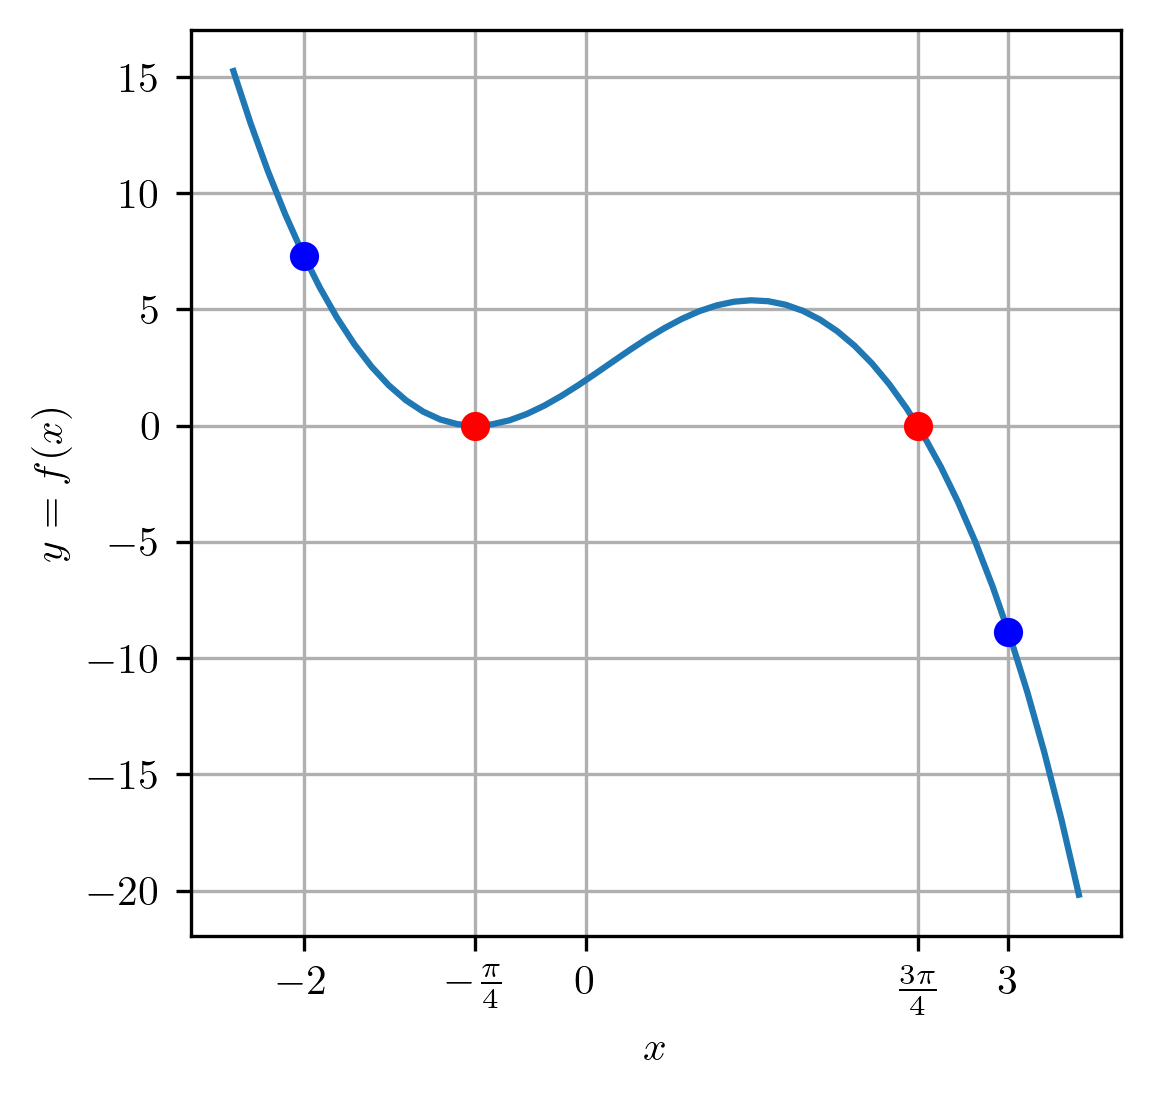
\includegraphics[width=0.8\textwidth]{./cap_eq1d/dados/fig_bis_intro/fig}
  \caption{Esboço da função $f$ do Exemplo~\ref{cap_eq1d_sec_bissec:ex:bis_intro}.}
  \label{cap_eq1d_sec_bissec:fig:bis_intro}
\end{figure}

Observamos que esta função é contínua e que, por exemplo, $f(-2)>0$ e $f(3)<0$, logo $f(-2)\cdot f(3) < 0$ e, de fato, $f$ tem pelo menos um zero\endnote{De fato, $f$ tem três zeros no intervalo $(-2, 3)$.} no intervalo $(-2, 3)$.
\end{ex}

Consideramos, então, uma função $f$ contínua tal que $f(a)\cdot f(b) < 0$. O \hl{método da bisseção é iterativo}, a primeira aproximação para uma solução de $f(x)=0$ é tomada como o ponto médio do intervalo $(a, b)$, i.e.
\begin{equation}
  x^{(0)} = \frac{a^{(1)}+b^{(1)}}{2},
\end{equation}
onde $a^{(0)} = a$ e $b^{(0)} = b$. Daí, se ocorrer $f(x^{(0)})=0$ o problema está resolvido. Caso contrário, $f$ tem pelo menos um zero num dos subintervalos $(a^{(0)}, x^{(0)})$ ou $(x^{(0)}, b^{(0)})$, pois $f(a^{(0)})\cdot f(x^{(0)}) < 0$ ou  $f(x^{(0)})\cdot f(b^{(0)}) < 0$, respectivamente e exclusivamente. No primeiro caso, escolhemos $(a^{(1)}, b^{(1)}) = (a^{(0)}, x^{(0)})$ ou, no segundo caso, tomamos $(a^{(1)}, b^{(1)}) = (x^{(0)}, b^{(0)})$. Então, a segunda aproximação para uma solução é computada como
\begin{equation}
  x^{(1)} = \frac{a^{(1)} + b^{(1)}}{2}.
\end{equation}
O procedimento se repete até obtermos uma aproximação com a precisão desejada.

\begin{ex}\label{cap_eq1d_sec_bissec:ex:bis_exec}
  Consideremos o problema de encontrar um zero da função
  \begin{equation}
    \begin{aligned}
      f(x) &= \sen^2\left(x+\frac{\pi}{4}\right) - x^3 \\
           &+ \frac{\pi}{4}x^2 + \frac{5\pi^2}{16}x + \frac{3\pi^3}{64}.
    \end{aligned}
\end{equation}
Do esboço de seu gráfico (Figura \ref{cap_eq1d_sec_bissec:fig:bis_intro}), observamos que $f(2)\cdot f(3) \neq 0$ sendo que o zero $x=3\pi/4\approx 2,3562$ de $f$ está no intervalo $(2, 3)$. Aplicando o método da bisseção com intervalo inicial $(a^{(0)}, b^{(0)}) = (2, 3)$ e aproximação inicial $x^{(0)} = (a^{(0)}+b^{(0)})/2$, obtemos as aproximações apresentadas na Tabela \ref{cap_eq1d_sec_bissec:tab:bis_exec}.

\begin{table}[h!]
  \centering
  \caption{Resultados referentes ao Exemplo~\ref{cap_eq1d_sec_bissec:ex:bis_exec}.}
  \begin{tabular}{r|rr|r|r}
    k & $a^{(k)}$ & $b^{(k)}$ & $x^{(k)}$ & $s$ \\\hline
    0 & $2,0000$ & $3,0000$ & $2,5000$ & -1 \\
    1 & $2,0000$ & $2,5000$ & $2,2500$ &  1 \\
    2 & $2,2500$ & $2,5000$ & $2,3750$ & -1 \\
    3 & $2,2500$ & $2,3750$ & $2,3125$ & 1 \\
    4 & $2,3125$ & $2,3750$ & $2,3438$ & 1 \\
    5 & $2,3438$ & $2,3750$ & $2,3594$ &  -1 \\
    6 & $2,3438$ & $2,3594$ & $2,3516$ & 1 \\
    7 & $2,3516$ & $2,3594$ & $2,3555$ &  1 \\
    8 & $2,3555$ & $2,3594$ & $2,3574$ &  -1 \\
    9 & $2,3555$ & $2,3574$ & $2,3564$ & -1 \\\hline
    \multicolumn{5}{r}{\small $s := f(a^{(k)})\cdot f(x^{(k)})$}
  \end{tabular}
  \label{cap_eq1d_sec_bissec:tab:bis_exec}
\end{table}

\begin{lstlisting}
import numpy as np

f = lambda x: np.sin(x+np.pi/4)**2 \
  - x**3 + np.pi/4*x**2 + 5*np.pi**2/16*x \
  + 3*np.pi**3/64

a = 2
b = 3
x = (a + b)/2
print(f"0: a={a:.4f}, b={b:.4f}, x={x:.4f}")
for k in range(9):
  s = np.sign(f(a)*f(x))
  if (s == -1):
    b = x
  elif (s == 1):
    a = x
  else:
    break
  x = (a + b)/2
  print(f"{k+1}: a={a:.4f}, b={b:.4f}, x={x:.4f}")
\end{lstlisting}

\end{ex}

\subsection{Análise Numérica}

Dada uma função contínua $f:[a, b]\to\mathbb{R}$ com $f(a)\cdot f(b) < 0$, vamos mostrar que o \hl{método da bisseção é \emph{globalmente convergente} e tem \emph{ordem de convergência linear}}.

\begin{defn}\normalfont{(\hl{Método Iterativo Globalmente Convergente}.)}
  Um método iterativo
  \begin{align}
    & x^{(0)} = \text{aprox. inicial},\\
    & x^{(k+1)} = g\left(x^{k}\right),
  \end{align}
  com $k = 0,1,\ldots$, é dito \emph{globalmente convergente}, quando
  \begin{equation}
    {\color{blue}\lim_{k\to\infty}\left|x^{(k+1)}-x^{(k)}\right| = 0}
  \end{equation}
  para qualquer escolha de $x^{(0)}$.
\end{defn}

\begin{defn}\normalfont{(\hl{Ordem de convergência}.)}
  Seja $\left(x^{(k)}\right)_{k=1}^\infty$ uma sequência convergente com
  \begin{equation}
    \lim_{k\to\infty} \left|x^{(k+1)}-x^{(k)}\right| = 0,
  \end{equation}
  com $x^{(k+1)}-x^{(k)}\neq 0$ para todo $k$. Dizemos que $\left(x^{(k)}\right)_{k=1}^\infty$ converge com ordem $\alpha>0$ e com constante de erro assintótica $C>0$, quando
  \begin{equation}
    {\color{blue}\lim_{k\to\infty}\frac{\left|x^{(k+1)}-x^*\right|}{\left|x^{(k)}-x^*\right|^\alpha} = C}. 
  \end{equation}
\end{defn}

Em geral, \hl{quando maior o valor de $\alpha$, mais rapidamente é a convergência das iteradas de um método iterativo}. Os seguintes casos são particularmente importantes:
\begin{itemize}
\item \hl{Se $\alpha = 1$ e $C < 1$, o método é \emph{linearmente convergente}}.
\item \hl{Se $\alpha = 2$, o método é \emph{quadraticamente convergente}}.
\end{itemize}

\subsubsection{Convergência e Precisão}

\begin{teo}\label{cap_eq1d_sec_bissec:teo:convp}
  Seja $f:[a, b]\to\mathbb{R}$ função contínua com $f(a)\cdot f(b) < 0$. Então, o \hl{método da bisseção é globalmente convergente}.
\end{teo}
\begin{dem}
  Seja $(x^{(k)})_{k=1}^\infty$ a sequência de aproximações\endnote{Caso, $f\left(a^{(k)}\right)=0$ ou $f\left(a^{(b)}\right)=0$, então assumimos que $a^{(k+i)} = a^{(k)}$ ou $b^{(k+i)} = b^{(k)}$, conforme o caso, para $i=1,2,3,\ldots$.} do método da bisseção. Por construção, temos
  \begin{align}
    \left|x^{(k)} - x^{(k-1)}\right| &\leq b^{(k-1)}-a^{(k-1)}\\
                                     &\leq \frac{b^{(k-2)}-a^{(k-2)}}{2}\\
                                     &\vdots\\
                                     &\leq \frac{b^{(0)}-a^{(0)}}{2^{k-1}}
  \end{align}
  Ou seja, obtemos a \hl{\emph{estimativa de convergência}}
  \begin{equation}\label{cap_eq1d_sec_bissec:eq:estconvp}
    {\color{blue}\left|x^{(k)} - x^{(k-1)}\right| \leq \frac{b^{(0)}-a^{(0)}}{2^{k-1}}}
  \end{equation}
  Daí, segue que
  \begin{align}
    \lim_{k\to\infty} \left|x^{(k)}-x^{(k-1)}\right| &= \lim_{k\to\infty} b^{(k)}-a^{(k-1)}\\
                                                     &= 0.
  \end{align}
\end{dem}

\begin{ex}\label{cap_eq1d_sec_bissec:ex:bis_convp}
  No Exemplo \ref{cap_eq1d_sec_bissec:ex:bis_exec} aplicamos o método da bisseção para a função
  \begin{equation}
    \begin{aligned}
      f(x) &= \sen^2\left(x+\frac{\pi}{4}\right) - x^3 \\
           &+ \frac{\pi}{4}x^2 + \frac{5\pi^2}{16}x + \frac{3\pi^3}{64}.
    \end{aligned}
\end{equation}
no intervalo $(2, 3)$. Ao recuperarmos os valores de $\left|x^{(k)}-x^{(k-1)}\right|$ obtemos
\begin{center}
  \begin{tabular}[H]{l|l|r}
    $k$ & $x^{(k)}$ & $\left|x^{(k)}-x^{(k-1)}\right|$\\\hline
    $0$ & $2.5000$ & -x-\\
    $1$ & $2.2500$ & $2,5\times 10^{-1}$\\
    $2$ & $2,3750$ & $1,2\times 10^{-1}$\\
    $3$ & $2,3125$ & $6,2\times 10^{-2}$\\
    $4$ & $2,3438$ & $3,1\times 10^{-2}$\\
    $5$ & $2,3594$ & $1,6\times 10^{-2}$\\
    $6$ & $2,3516$ & $7,8\times 10^{-3}$\\
    $7$ & $2,3555$ & $3,9\times 10^{-3}$\\
    $8$ & $2,3574$ & $2,0\times 10^{-3}$\\
    $9$ & $2,3564$ & $9,8\times 10^{-4}$\\\hline
  \end{tabular}
\end{center}

Observamos que os valores estão de acordo com a estimativa de convergência \ref{cap_eq1d_sec_bissec:eq:estconvp}, donde
\begin{align}
  |x^{(9)}-x^{(8)}| &\leq \frac{b^{(0)}-a^{(0)}}{2^{9}}\\
                     &= \frac{3 - 2}{2^{9}} = 1.9\times 10^{-3}
\end{align}
\end{ex}

O \hl{Teorema~{\ref{cap_eq1d_sec_bissec:teo:convp}} nos garante a convergência do método da bisseção e uma estimativa de \emph{precisão}} (Equação~\ref{cap_eq1d_sec_bissec:eq:estconvp}). O teorema \hl{não garante que} o método \hl{converge para um zero da função objetivo}, apenas garante que as aproximações convergem para algum valor no intervalo inicial dado.

\subsubsection{Convergência e Exatidão}

Dada uma \hl{função contínua e estritamente monótona}\endnote{Função estritamente crescente ou estritamente decrescente, exclusivamente.} \hl{$f:[a, b]\to\mathbb{R}$ com $f(a)\cdot f(b) < 0$}, temos que o método da bisseção converge para o zero de $f$ em $[a, b]$.

\begin{teo}\label{cap_eq1d_sec_bissec:teo:bissece}
  Seja $f:[a, b]\to\mathbb{R}$ função contínua e estritamente monótona com $f(a)\cdot f(b) < 0$. Então, o \hl{método da bisseção converge para o zero de $f$ em $[a, b]$}.
\end{teo}
\begin{dem}
  Das hipóteses temos que $f$ tem um único zero $x^*$ em $(a, b)$. Seja $(x^{(k)})_{k=1}^\infty$ a sequência de aproximações\endnote{Caso, $f\left(a^{(k)}\right)=0$ ou $f\left(a^{(b)}\right)=0$, então assumimos que $a^{(k+i)} = a^{(k)}$ ou $b^{(k+i)} = b^{(k)}$, conforme o caso, para $i=1,2,3,\ldots$.} do método da bisseção. Por construção, temos
  \begin{align}
    |x^{(k)} - x^{*}| &\leq \frac{b^{(k)}-a^{(k)}}{2}\\
                      &\leq \frac{b^{(k-1)}-a^{(k-1)}}{2^2}\\
                      &\vdots \\
                      &\leq \frac{b^{(1)}-a^{(1)}}{2^k},
  \end{align}
  donde, obtemos a seguinte estimativa do \hl{\emph{erro de truncamento}}
  \begin{equation}\label{cap_eq1d_sec_bissec:eq:bis_est_trunc}
    {\color{blue}|x^{(k)} - x^{*}| \leq \frac{b^{(1)}-a^{(1)}}{2^k}}.
  \end{equation}
  E, daí também, segue que o método converge para o zero de $f$, pois
  \begin{equation}
    \lim_{k\to\infty} |x^{(k)}-x^{*}| = \lim_{k\to\infty} \frac{b^{(1)}-a^{(1)}}{2^k} = 0.
  \end{equation}
\end{dem}

\begin{obs}(\normalfont{\hl{Estimativa de Exatidão}.)}
  A estimativa de truncamento \ref{cap_eq1d_sec_bissec:eq:bis_est_trunc} é também um \emph{estimativa de exatidão}, i.e. nos fornece uma medida do erro na $k$-ésima aproximação do método da bisseção.
\end{obs}

\begin{ex}\label{cap_eq1d_sec_bissec:ex:bis_convp}
  No Exemplo \ref{cap_eq1d_sec_bissec:ex:bis_exec} aplicamos o método da bisseção para a função
  \begin{equation}
    \begin{aligned}
      f(x) &= \sen^2\left(x+\frac{\pi}{4}\right) - x^3 \\
           &+ \frac{\pi}{4}x^2 + \frac{5\pi^2}{16}x + \frac{3\pi^3}{64}.
    \end{aligned}
\end{equation}
no intervalo $(2, 3)$. A aplicação do método, nos fornece
\begin{center}
  \begin{tabular}[H]{llr}
    $k$ & $x^{(k)}$ & $\left|x^{(k)}-x^{*}\right|$\\\hline
    $0$ & $2.3560$ & $1.4\times 10^{-1}$ \\
    $1$ & $2.2500$ & $1.1\times 10^{-1}$ \\
    $2$ & $2.3750$ & $1.9\times 10^{-2}$ \\
    $3$ & $2.3125$ & $4.4\times 10^{-2}$ \\
    $4$ & $2.3438$ & $1.2\times 10^{-2}$ \\
    $5$ & $2.3594$ & $3.2\times 10^{-3}$ \\
    $6$ & $2.3516$ & $4.6\times 10^{-3}$ \\
    $7$ & $2.3555$ & $7.3\times 10^{-4}$ \\
    $8$ & $2.3574$ & $1.2\times 10^{-3}$ \\
    $9$ & $2.3564$ & $2.5\times 10^{-4}$ \\\hline
  \end{tabular}
\end{center}
onde, $x^* = x_1 = 3\pi/4$. Observamos que este resultado é consistente com a estimativa do erro de truncamento \eqref{cap_eq1d_sec_bissec:eq:bis_est_trunc}, da qual temos
\begin{align}
  |x^{(9)} - x^*| &\leq \frac{b^{(0)}-a^{(0)}}{2^{10}}\\
                  &= \frac{1}{2^{10}} = 1,0\E-3.
\end{align}
\end{ex}

\begin{obs}\normalfont{(\hl{Ordem de Convergência Linear}.)}
  A estimativa de convergência \eqref{cap_eq1d_sec_bissec:eq:bis_est_trunc} também pode ser usada para mostrarmos que, assintoticamente, o método da bisseção tem a seguinte taxa de convergência linear
  \begin{equation}
    \left|x^{(k+1)} - x^{(k)}\right| \lesssim \frac{1}{2}\left|x^{(k)} - x^{(k-1)}\right|^{\pmb{1}}.
  \end{equation}
\end{obs}

\subsection{Zeros de Multiplicidade Par}

Sejam \hl{$f$ uma função suave e $x^*$ um zero de multiplicidade par de $f$}. Observamos que o \hl{método da bisseção não é diretamente aplicável} para aproximar $x^*$. Isto ocorre, pois, neste caso, $x^*$ será um ponto de mínimo ou de máximo local de $f$, não havendo pontos $a$ e $b$ próximos de $x^*$ tal que $f(a)\cdot f(b) < 0$.

Agora, \hl{sendo $x^*$ um zero de $f$ de multiplicidade $2m$}, temos que ela admite a seguinte decomposição
\begin{equation}
  f(x) = (x-x^*)^{2m}g(x),
\end{equation}
onde $g$ é uma função suave e $g(x^*)\neq 0$. Daí, a derivada de $f$
\begin{equation}
  f'(x) = 2m(x-x^*)^{2m-1}g(x) + (x-x^*)^{2m}g'(x),
\end{equation}
tem $x^*$ como um zero de multiplicidade $2m-1$ (ímpar) e, desta forma, \hl{podemos aplicar o método da bisseção em $f'$ para aproximar $x^*$}.

\begin{ex}\label{cap_eq1d_sec_bissec:ex:bis_multpar}
  A função
  \begin{equation}
    \begin{aligned}
      f(x) &= \sen^2\left(x+\frac{\pi}{4}\right) - x^3 \\
           &+ \frac{\pi}{4}x^2 + \frac{5\pi^2}{16}x + \frac{3\pi^3}{64}.
    \end{aligned}
\end{equation}
tem $x=-\pi/4\approx -0,7854$ como um zero de multiplicidade par (veja Figura \ref{cap_eq1d_sec_bissec:fig:bis_multpar}).

\begin{figure}[H]
  \centering
  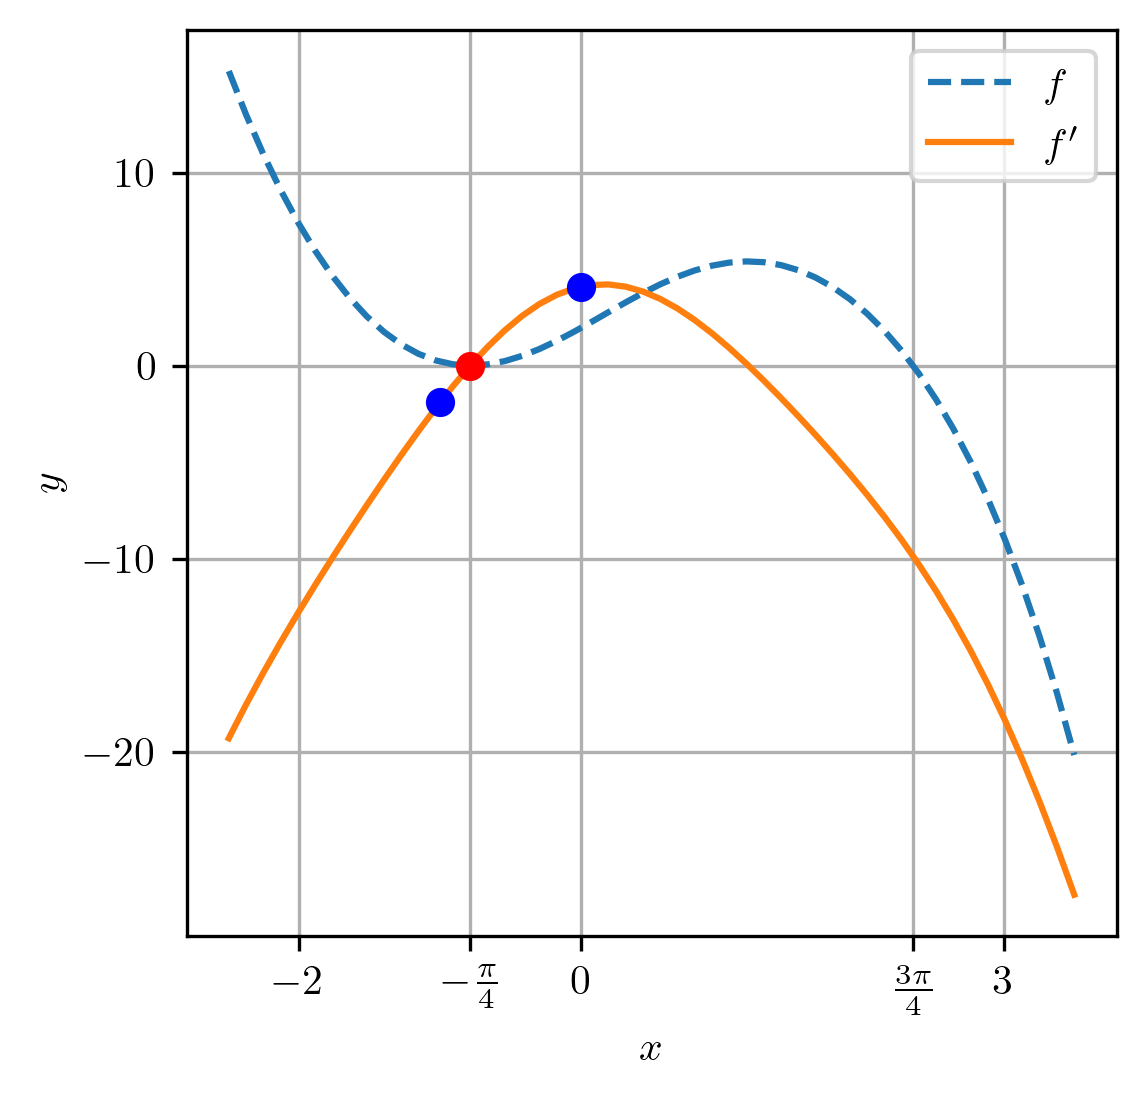
\includegraphics[width=0.8\textwidth]{./cap_eq1d/dados/fig_bis_multpar/fig}
  \caption{Esboço do gráfico da $f$ e de sua derivada $f'$ dada no Exemplo \ref{cap_eq1d_sec_bissec:ex:bis_multpar}.}
  \label{cap_eq1d_sec_bissec:fig:bis_multpar}
\end{figure}

Para aplicarmos o método da bisseção para aproximarmos este zero, primeiramente, derivamos $f$
\begin{equation}
  \begin{aligned}
    f'(x) &= 2\sin(x+\pi/4)\cos(x+\pi/4) - 3x^2 \\
          &+ \frac{\pi}{2}x + \frac{5\pi^2}{16}.
  \end{aligned}
\end{equation}
O esboço do gráfico de $f'$ (Figura \ref{cap_eq1d_sec_bissec:fig:bis_multpar}) mostra que $f'(-1)\cdot f'(0) < 0$ sendo que no intervalo $(-1, 0)$ $f'$ tem um zero de multiplicidade ímpar. Então, aplicando o método da bisseção a $f'$ no intervalo inicial $(a^{(1)}, b^{(1)}) = (-1, ~0)$, obtemos os resultados apresentados na Tabela~\ref{cap_eq1d_sec_bissec:tab:bis_multpar}. Nesta tabela são apresentados as iteradas até a convergência da solução com precisão de $10^{-3}$.

\begin{table}[H]
  \centering
  \caption{Resultados referentes ao Exemplo~\ref{cap_eq1d_sec_bissec:ex:bis_exec}.}
  \begin{tabular}{r|rr|r|r}
    k & $a^{(k)}$ & $b^{(k)}$ & $x^{(k)}$ & $s$\\\hline
    0 & $-1,0000\E+0$ & $0,0000\E+0$ & $-5,0000\E-1$ & -1 \\
    1 & $-1,0000\E+0$ & $-5,0000\E-1$ & $-7,5000\E-1$ & -1 \\
    2 & $-1,0000\E+0$ & $-7,5000\E-1$ & $-8,7500\E-1$ & 1 \\
    3 & $-8,7500\E-1$ & $-7,5000\E-1$ & $-8,1250\E-1$ &  1 \\
    4 & $-8,1250\E-1$ & $-7,5000\E-1$ & $-7,8125\E-1$ & -1 \\
    5 & $-8,1250\E-1$ & $-7,8125\E-1$ & $-7,9688\E-1$ & 1 \\
    6 & $-7,9688\E-1$ & $-7,8125\E-1$ & $-7,8906\E-1$ & 1 \\
    7 & $-7,8906\E-1$ & $-7,8125\E-1$ & $-7,8516\E-1$ & -1 \\
    8 & $-7,8906\E-1$ & $-7,8516\E-1$ & $-7,8711\E-1$ & 1 \\
    9 & $-7,8711\E-1$ & $-7,8516\E-1$ & $-7,8613\E-1$ & 1 \\\hline
    \multicolumn{5}{r}{\small $s := f'(a^{(k)})\cdot f'(x^{(k)})$}
  \end{tabular}
  \label{cap_eq1d_sec_bissec:tab:bis_multpar}
\end{table}
\end{ex}

\subsection{Exercícios}

\begin{exer}
  Use o método da bisseção para aproximar um zero de
  \begin{equation}
    f(x)=x^3\sen(x)-\cos(x)
\end{equation}
aplicando como intervalo inicial $(a^{(0)}, b^{(0)}) = (0,5, ~1)$ e aproximação inicial $x^{(0)}=(a^{(0)}+b^{(0)})/2$. Faça, então, $6$ iterações de forma a obter a aproximação $x^{(6)}$ e forneça-a com $7$ dígitos significativos por arredondamento.
\end{exer}
\begin{resp}
  $9,179688\times 10^{-1}$
\end{resp}

\begin{exer}
  Considere o método da bisseção para aproximar um zero de $f(x)=x^3\sen(x)-\cos(x)$, aplicando como intervalo inicial $(a^{(0)}, b^{(0)}) = (0,5, ~1)$ e aproximação inicial $x^{(0)}=(a^{(0)}+b^{(0)})/2$. Use a estimativa de convergência \eqref{cap_eq1d_sec_bissec:eq:bis_est_trunc}
  \begin{equation}
    \left|x^{(k)} - x^{*}\right| \leq \frac{b^{(0)}-a^{(0)}}{2^k},
  \end{equation}
para estimar o número mínimo de iterações $k_{conv}$ necessárias para se obter a solução com exatidão de $10^{-4}$. Então, compute $x^{(k_{conv})}$ e forneça-o com $6$ dígitos significativos por arredondamento.
\end{exer}
\begin{resp}
  $9,15833\E-1$
\end{resp}

\begin{exer}
  Use o método da bisseção para computar a(s) solução(ões) das seguintes equações com precisão de 8 dígitos significativos.
  \begin{enumerate}[a)]
  \item $x = 2^{-x}$ para $0\leq x \leq 2$.
  \item $e^{-x^2} = 3x - x^2$ para $-1\leq x\leq 4$.
  \end{enumerate}
\end{exer}
\begin{resp}
  a) $6.4118574\times 10^{-1}$; b) $3.3536470\times 10^{-1}$; $2.9999589$
\end{resp}

\begin{exer}
  Use o método da bisseção para encontrar uma aproximação com precisão de $10^{-4}$ do zero de
  \begin{align}
    f(x) &= (-x^2+1,154x-0,332929)\cos(x) + x^2 \nonumber\\
         &- 1,154x + 0,332929
  \end{align}
no intervalo $(0,55, ~0,65)$. Forneça a aproximação computada com $7$ dígitos significativos por arredondamento.
\end{exer}
\begin{resp}
  $5,770508\times 10^{-1}$
\end{resp}

\begin{exer}
  Aplique o método da bisseção para encontrar o ponto crítico\endnote{Definimos que $x$ é ponto crítico de uma dada $f$, quando $f'(x) = 0$ ou $\nexists f'(x)$.} de
  \begin{equation}
    f(x) = (1-x^2)e^{-x^2}
  \end{equation}
  no intervalo $(0, 2)$. Obtenha o resultado com precisão de $5$ dígitos significativos por arredondamento.
\end{exer}
\begin{resp}
  $1,4142\E+0$
\end{resp}

\ifisbook
\subsubsection{Respostas}
\shipoutAnswer
\fi

%%% SECTION %%%

\section{Método da Falsa Posição}\label{cap_eq1d_sec_falsapos}

O método da falsa posição \hl{é uma variação do método da bisseção}. Dada uma função $f$ contínua, escolhemos um intervalo inicial $(a, b)$ tal que $f(a)\cdot f(b) < 0$ (i.e. \hl{$f$ tem sinais trocados nos pontos $a$ e $b$}). Então, uma \hl{aproximação para o zero de $f$} neste intervalo \hl{é computada como o ponto de interseção da reta secante a $f$ pelos pontos $(a, f(a))$ e $(b, f(b))$}, i.e.
\begin{equation}
  x = a - \frac{b-a}{f(b)-f(a)}f(a).
\end{equation}
Veja a Figura \ref{cap_eq1d_sec_falsapos:fig:falsapos}.

\begin{figure}[H]
  \centering
  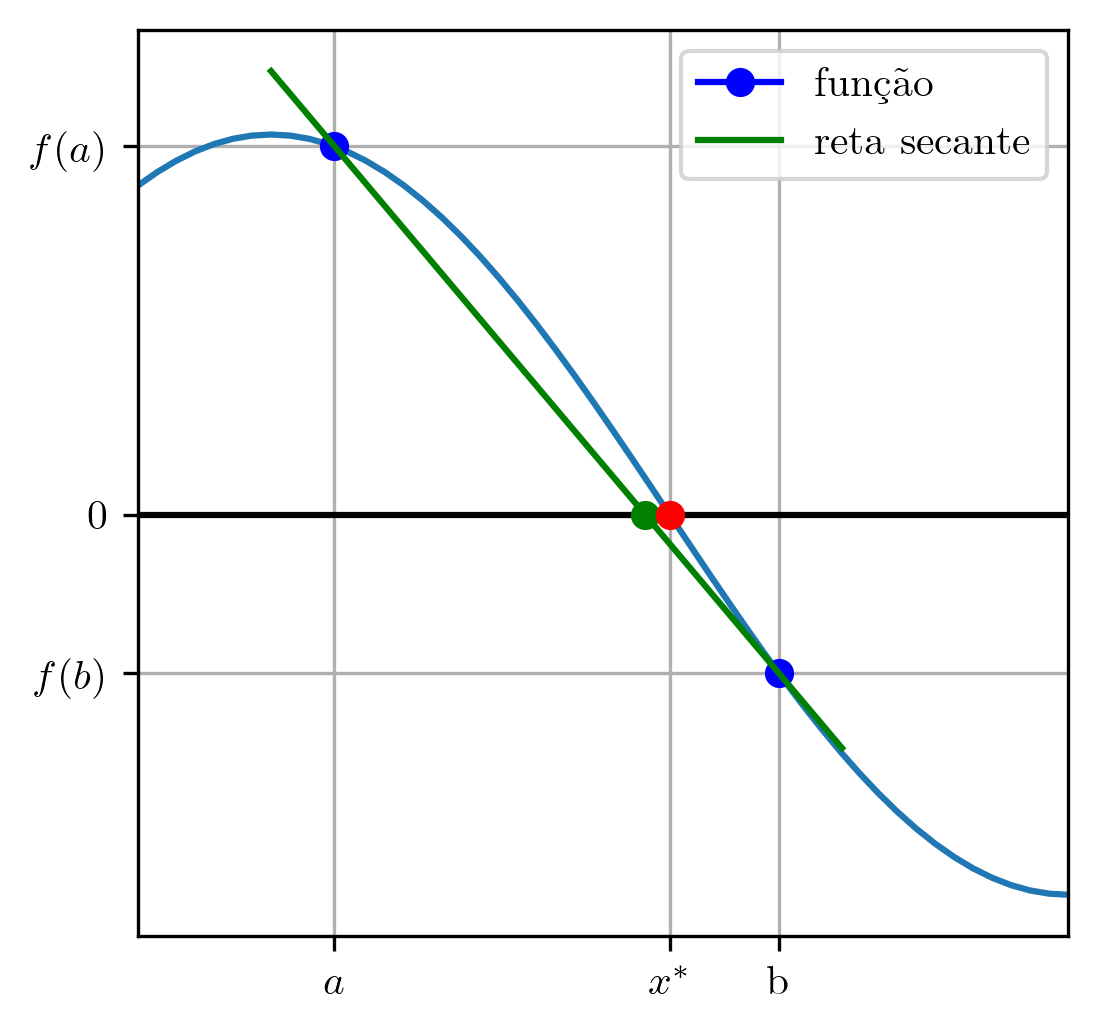
\includegraphics[width=0.7\textwidth]{./cap_eq1d/dados/fig_falsapos/fig}
  \caption{Ilustração do método da falsa posição.}
  \label{cap_eq1d_sec_falsapos:fig:falsapos}
\end{figure}

Mais explicitamente, \hl{o método consiste no seguinte procedimento iterativo}:
\begin{enumerate}
\item Determinar um intervalo $(a^{(1)}, b^{(1)})$ tal que $f(a^{(1)})\cdot f(b^{(1)}) < 0$.
\item Para $k = 1, 2, 3, \cdots, N$:
  \begin{enumerate}[2.1]
  \item $\displaystyle x^{(k)} = a^{(k)} - \frac{b^{(k)}-a^{(k)}}{f(b^{(k)})-f(a^{(k)})}f(a^{(k)})$
  \item Verificar critério de parada.
  \item Se $f(a^{(k)})\cdot f(x^{(k)}) < 0$, então $a^{(k+1)}=a^{(k)}$ e $b^{(k+1)}=x^{(k)}$.
  \item Se $f(x^{(k)})\cdot f(b^{(k)}) > 0$, então $a^{(k+1)}=x^{(k)}$ e $b^{(k+1)}=b^{(k)}$.
  \end{enumerate}
\end{enumerate}

\begin{ex}
  Consideremos o problema de aproximar o zero de
  \begin{equation}
    \begin{aligned}
      f(x) &= \sen^2\left(x+\frac{\pi}{4}\right) - x^3 \\
           &+ \frac{\pi}{4}x^2 + \frac{5\pi^2}{16}x + \frac{3\pi^3}{64}.
    \end{aligned}
\end{equation}
no intervalo $(0, 3)$. A tabela abaixo mostra os resultados obtidos da aplicação do método da falsa posição com intervalo inicial $(a^{(1)}, b^{(1)}) = (2, 3)$. Aqui, o método foi iterado até a convergência com cinco dígitos significativos.

\begin{center}
  \begin{tabular}{r|rr|r|r}
    k & $a^{(k)}$ & $b^{(k)}$ & $x^{(k)}$ & $s$\\\hline
    0 & $2,0000$ & $3,0000$ & $2,2455$ & 1 \\
    1 & $2,2455$ & $3,0000$ & $2,3240$ &  1 \\
    2 & $2,3240$ & $3,0000$ & $2,3470$ & 1 \\
    3 & $2,3470$ & $3,0000$ & $2,3536$ & 1 \\
    4 & $2,3536$ & $3,0000$ & $2,3555$ & 1 \\
    5 & $2,3555$ & $3,0000$ & $2,3560$ & 1 \\
    6 & $2,3560$ & $3,0000$ & $2,3561$ &  1 \\
    7 & $2,3561$ & $3,0000$ & $2,3562$ & 1 \\
    8 & $2,3562$ & $3,0000$ & $2,3562$ & 1 \\
    9 & $2,3562$ & $3,0000$ & $2,3562$ & 1 \\\hline
    \multicolumn{5}{r}{\small $s := f'(a^{(k)})\cdot f'(x^{(k)})$}
  \end{tabular}
\end{center}

\begin{lstlisting}
import numpy as np

f = lambda x: np.sin(x+np.pi/4)**2 \
  - x**3 + np.pi/4*x**2 + 5*np.pi**2/16*x \
  + 3*np.pi**3/64

a = 2.
b = 3.
for k in range(10):
  x = a - (b-a)/(f(b)-f(a))*f(a)
  print(f"{k+1}: {x:.4f}")

  s = np.sign(f(a)*f(x))
  if (s == -1):
    b = x
  elif (s == 1):
    a = x
  else:
    break
\end{lstlisting}
\end{ex}

\begin{obs}\normalfont{(\hl{Ordem de Convergência}.)}
  O método da falsa posição é \emph{globalmente convergente} e tem \emph{ordem de convergência linear} \cite[Seção 8.3]{Ralston2001a}.
\end{obs}

\subsection{Exercícios}

\begin{exer}
  Use o método da falsa posição para aproximar um zero de
  \begin{equation}
    f(x) = x^3\sen(x)-\cos(x)
  \end{equation}
  aplicando, como intervalo inicial $(a^{(1)}, b^{(1)}) = (0,5, ~1)$ e aproximação inicial
  \begin{equation}
    x^{(0} = a^{(1)} - \frac{b^{(1)}-a^{(1)}}{f(b^{(1)})-f(a^{(1)})}f(a^{(1)}).
  \end{equation}
  Faça, então, $4$ iterações deste método de forma a obter a aproximação $x^{(4)}$ e forneça-a com $7$ dígitos significativos por arredondamento.
\end{exer}
\begin{resp}
  $9,158079\times 10^{-1}$
\end{resp}

\begin{exer}
  Use o método da falsa posição para computar a(s) solução(ões) das seguintes equações com precisão de 8 dígitos significativos.
  \begin{enumerate}[a)]
  \item $x = 2^{-x}$ para $0\leq x \leq 2$.
  \item $e^{-x^2} = 3x - x^2$ para $-1\leq x\leq 4$.
  \end{enumerate}
\end{exer}
\begin{resp}
  a) $6.4118574\times 10^{-1}$; b) $3.3536470\times 10^{-1}$; $2.9999589$
\end{resp}

\begin{exer}
  Use o método da falsa posição para encontrar uma aproximação com precisão de $4$ dígitos significativos do zero de 
  \begin{equation}
    \begin{aligned}
      f(x) &= (-x^2+1,154x-0,332929)\cos(x) + x^2 \\
           &- 1,154x + 0,332929
    \end{aligned}
\end{equation}
  no intervalo $[-1, 0]$.
\end{exer}
\begin{resp}
  $-7,861\times 10^{-1}$
\end{resp}

\begin{exer}
  Use o método da falsa posição para encontrar uma aproximação com precisão de $10^{-4}$ do zero de
  \begin{equation}
    \begin{aligned}
      f(x) &= (-x^2+1,154x-0,332929)\cos(x) + x^2 \\
           &- 1,154x + 0,332929
    \end{aligned}
\end{equation}
no intervalo $(0,55, ~0,65)$. Forneça a aproximação computada com $7$ dígitos significativos por arredondamento.
\end{exer}
\begin{resp}
  $5,770508\times 10^{-1}$
\end{resp}

\begin{exer}
  Aplique o método da falsa posição para encontrar o ponto crítico\endnote{Definimos que $x$ é ponto crítico de uma dada $f$, quando $f'(x) = 0$ ou $\nexists f'(x)$.} de
  \begin{equation}
    f(x) = (1-x^2)e^{-x^2}
  \end{equation}
  no intervalo $(0, 2)$. Obtenha o resultado com precisão de $5$ dígitos significativos por arredondamento.
\end{exer}

\ifisbook
\subsubsection{Respostas}
\shipoutAnswer
\fi

%%% SECTION %%%

\section{Iteração de Ponto Fixo}\label{cap_eq1d_sec_pfixo}

\hl{Um \emph{ponto fixo de uma função} $g$ é um ponto $x$ tal que}
\begin{equation}\hleq
  g(x) = x.
\end{equation}
Geometricamente, \hl{pontos fixos são interseções do gráfico da $g$ com a reta $y=x$}, veja a Figura \ref{cap_eq1d_sec_pfixo:fig:pfixo}.

\begin{figure}[H]
  \centering
  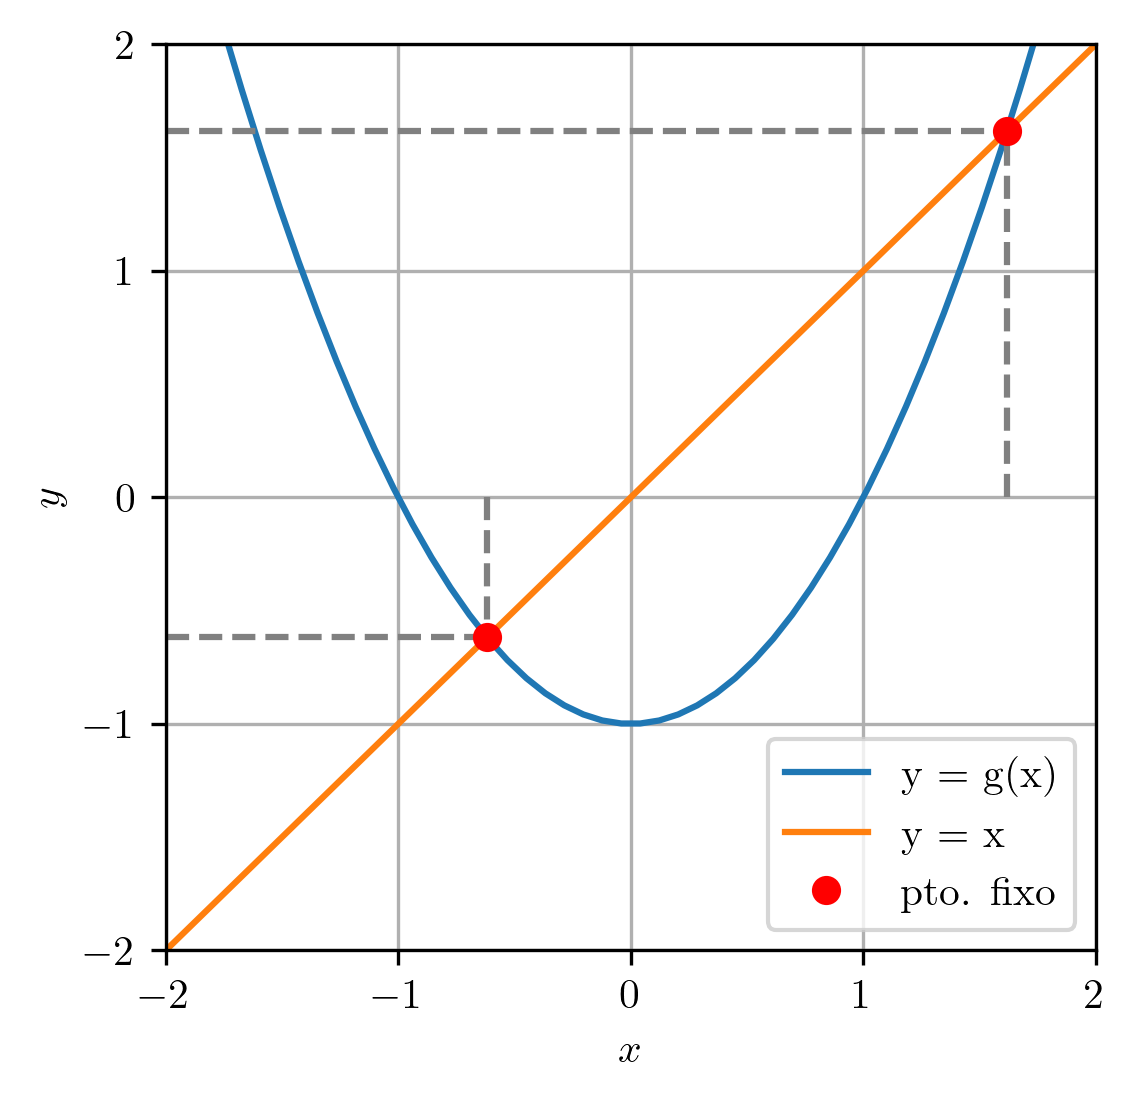
\includegraphics[width=0.8\textwidth]{./cap_eq1d/dados/fig_pfixo/fig}
  \caption{Exemplos de pontos fixos.}
  \label{cap_eq1d_sec_pfixo:fig:pfixo}
\end{figure}

Observamos que \hl{toda equação de uma incógnita pode ser reescrita} de forma equivalente \hl{como um problema de ponto fixo}.

\begin{ex}\label{cap_eq1d_sec_pfixo:ex:pfixo_intro}
  Consideremos o problema de resolver
  \begin{equation}
    \begin{aligned}
      &\sen^2\left(x+\frac{\pi}{4}\right) = x^3 - \frac{\pi}{4}x^2 \\
      &\qquad - \frac{5\pi^2}{16}x - \frac{3\pi^3}{64}.
    \end{aligned}
\end{equation}
Podemos reescrevê-la como o problema de se obter os zeros da seguinte função
\begin{equation}
  \begin{aligned}
    f(x) &= \sen^2\left(x+\frac{\pi}{4}\right) - x^3 \\
         &+ \frac{\pi}{4}x^2 + \frac{5\pi^2}{16}x + \frac{3\pi^3}{64}.
  \end{aligned}
\end{equation}
Por sua vez, este problema é equivalente aos seguintes problemas de ponto fixo (entre outros):
\begin{enumerate}[a)]
\item
  \begin{equation}
    \begin{aligned}
      g_1(x) &= \frac{16}{5\pi^2}\left[-\sen^2\left(x+\frac{\pi}{4}\right) + x^3 \right. \\
             &\left. - \frac{\pi}{4}x^2 - \frac{3\pi^3}{64}\right] = x.
    \end{aligned}
  \end{equation}
\item
  \begin{equation}
    \begin{aligned}
      g_2(x) &= \left[\sen^2\left(x+\frac{\pi}{4}\right) + \frac{\pi}{4}x^2\right. \\
             &\left. + \frac{5\pi^2}{16}x + \frac{3\pi^3}{64}\right]^{\frac{1}{3}} = x
    \end{aligned}
\end{equation}
\end{enumerate}
Na Figura \ref{cap_eq1d_sec_pfixo:fig:ex_pfixo_intro} podemos observar que os zeros da $f$ (a saber, $x_1=3\pi/4\approx 2,3562$ e $x_2=x_3=-\pi/4\approx -0,78540$) coincidem com os pontos fixos das funções $g_1$ e $g_2$.

\begin{figure}[H]
  \centering
  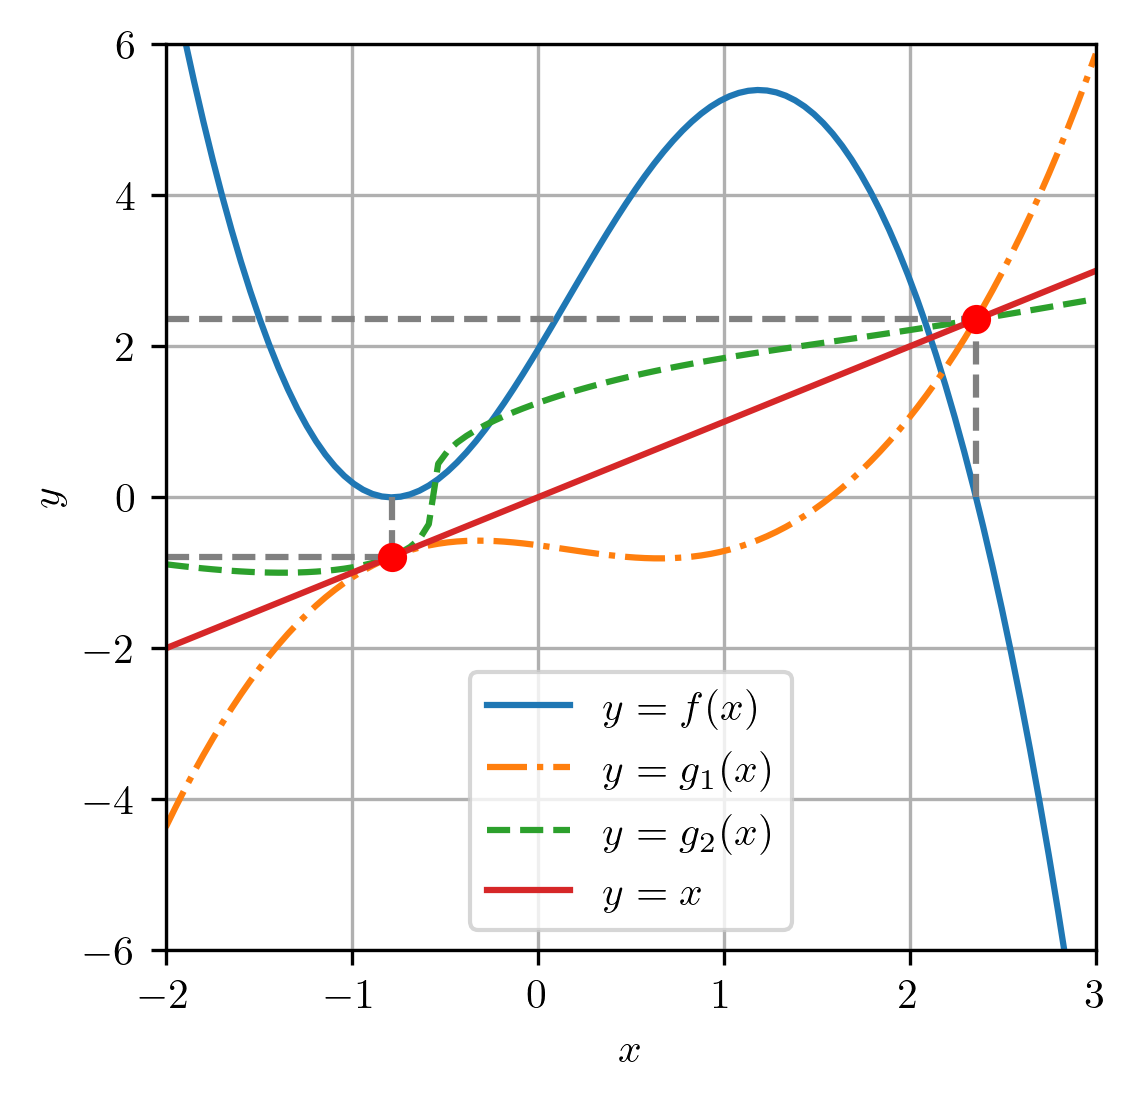
\includegraphics[width=0.8\textwidth]{./cap_eq1d/dados/fig_ex_pfixo_intro/fig}
  \caption{Esboço da função $f$, $g_1$ e $g_2$ do Exemplo~\ref{cap_eq1d_sec_pfixo:ex:pfixo_intro}.}
  \label{cap_eq1d_sec_pfixo:fig:ex_pfixo_intro}
\end{figure}
\end{ex}

Em muitos casos, é possível obter aproximações de um ponto fixo de uma dada função $g$ pela chamada \hl{\emph{iteração de ponto fixo}}:
\begin{align}
  {\color{blue}x^{(0)}} &{\color{blue}= \text{aprox. inicial}},\\
  {\color{blue}x^{(k+1)}} &{\color{blue}= g(x^{(k)})},
\end{align}
com $k=0,1,2,\ldots$.

\begin{ex}
  Vamos estudar as seguintes iterações de ponto fixo com as funções $g1$ e $g_2$ consideradas no Exemplo~\ref{cap_eq1d_sec_pfixo:ex:pfixo_intro}.
  \begin{enumerate}[a)]
  \item Função $g_1$ com $x^{(0)} = 0,7$.
    \begin{align}
      x^{(0)} &= -0,70000,\\
      x^{(1)} &= g_1\left(x^{(0)}\right)\\
              &= -0,70959,\\
      x^{(2)} &= g_1\left(x^{(1)}\right)\\
              &=-0,71716,\\
              &\vdots \nonumber\\
      x^{(99)} &= g_1\left(x^{(98)}\right)\\
              &= -0,77862,\\
              &\vdots \nonumber\\
      x^{(999)} &= g_1\left(x^{(998)}\right)\\
              &= -0,78466,\\    
              &\vdots \nonumber\\
      x^{(19999)} &= g_1\left(x^{(19998)}\right)\\
              &= -0,78536.
    \end{align}
    Neste caso as iterações de ponto fixo convergem (lentamente) para o ponto fixo $x=-\pi/4\approx -0,78540$.

  \item Função $g1$ com $x^{(0)} = 2,5$.
    
    Este valor inicial está próximo do ponto fixo $x=3\pi/4\approx 2,3562$, entretanto as iterações de ponto fixo divergem:
    \begin{align}
      x^{(0)} &= 2,50000,\\
      x^{(1)} &= g_1\left(x^{(0)}\right)\\
              &= 2,9966,\\
      x^{(2)} &= 5,8509,\\
              &\vdots \nonumber\\
      x^{(7)} &= 4,8921\times 10^{121}.
    \end{align}
    
  \item Função $g_2$ com $x^{(0)} = 2,5$.
    Neste caso, as iterações de ponto fixo convergem (rapidamente) para o ponto fixo próximo:
    \begin{align}
      x^{(0)} &= 2,50000,\\
      x^{(1)} &= g_2\left(x^{(0)}\right)\\
              &= 2,4155,\\
      x^{(2)} &= 2,3805,\\
              &\vdots \\
      x^{(9)} &= 2,3562.
    \end{align}    
  \end{enumerate}
\end{ex}

Este último exemplo mostra que a iteração do ponto fixo nem sempre é convergente. Antes de vermos condições suficientes para a convergência, vejamos sua interpretação geométrica.

\subsection{Interpretação Geométrica}

A Figura \ref{cap_eq1d_sec_pfixo:fig:pfixo_interp} apresenta o caso de uma iteração de ponto fixo convergente. As iterações iniciam-se no ponto $x^{(0)}$ e seguem para $x^{(1)} = g(x^{(0)})$ e $x^{(2)} = g(x^{(1)})$.

\begin{figure}[H]
  \centering
  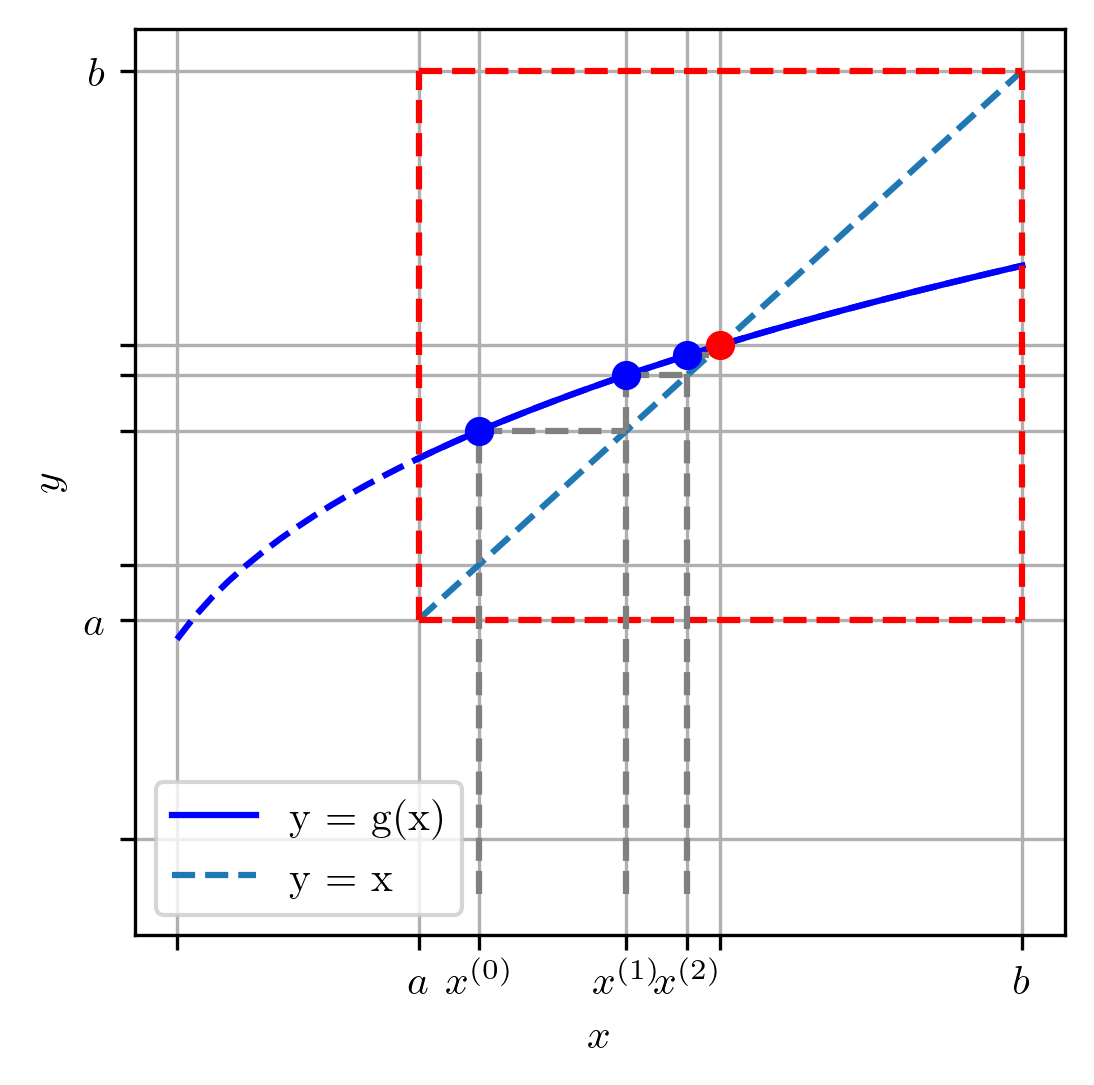
\includegraphics[width=\textwidth]{./cap_eq1d/dados/fig_pfixo_interp/fig}
  \caption{Interpretação geométrica da iteração de ponto fixo.}
  \label{cap_eq1d_sec_pfixo:fig:pfixo_interp}
\end{figure}

\subsection{Análise Numérica}

O seguinte teorema nos fornece condições suficientes para a convergência das iterações de ponto fixo.

\begin{teo}\normalfont{(\hl{Teorema do Ponto Fixo}.)}\label{cap_eq1d_sec_pfixo:teo:pfixo}
  Seja $g$ função continuamente diferenciável satisfazendo ambas as seguintes condições
  \begin{enumerate}[a)]
  \item $g\left([a, b]\right) \subset [a, b]$,
  \item $|g'(x)|<K<1$ para todo $x\in [a, b]$.
  \end{enumerate}
  Então, $g$ tem um único ponto fixo $x^*\in [a, b]$ e as iterações
  \begin{equation}
    x^{(k+1)}= g\left(x^{(k)}\right), k=0, 1, 2, \ldots,
  \end{equation}
  convergem para $x^*$, para qualquer escolha de $x^{(0)}\in [a, b]$.
\end{teo}
\begin{dem}
  Da hipótese b), temos que $g$ é uma contração com
  \begin{equation}
    \left|g(x) - g(y)\right| < K\cdot |x - y|,
  \end{equation}
  para quaisquer $x,y\in [a, b]$. Com isso, da hipótese a) e tomando $x^{(0)}\in [a, b]$, temos
  \begin{align}
    \left|x^{(k+1)} - x^{(k)}\right| &= \left|g(x^{(k)}) - g(x^{(k-1)})\right|\\
                                     &\leq K \left|x^{(k)} - x^{(k-1)}\right|\\
                                     &\vdots \nonumber\\
                                     &\leq K^{k-1}\left|x^{(2)}-x^{(1)}\right|,
  \end{align}
  para $k=1, 2, \ldots$. Como $K<1$, temos $\left|x^{(k+1)}-x^{(k)}\right|\to 0$ quando $k\to\infty$ e, portanto, $x^{(k)}$ converge para algum $x^*\in [a, b]$.
  
  De fato, $x^*$ é ponto fixo de $g$, pois da continuidade da $g$, temos
  \begin{align}
    x^* &= \lim_{k\to\infty} x^{(k+1)}\\
        &= \lim_{k\to\infty} g(x^{(k)}) = g(x^*).
  \end{align}
  
  Por fim, $x^*$ é único, pois assumindo a existência de outro ponto fixo $x^{**}\neq x^*$ teríamos
  \begin{align}
    |x^* - x^{**}| &= |g(x^*) - g(x^{**})| \\
                   &< K|x^* - x^{**}|\\
                   &< |x^* - x^{**}|.
  \end{align}
\end{dem}

\begin{obs}\normalfont{(Ordem de Convergência.)}
  A \hl{iteração de ponto fixo tem ordem de convergência linear}
  \begin{equation}
    |x^{(k+1)} - x^{(k)}| < K|x^{(k)} - x^{(k-1)}|^{\pmb{1}},
  \end{equation}
onde $0 < K < 1$ é a constante dada na hipótese $b)$ do Teorema do Ponto Fixo. Além disso, isso mostra que \hl{quanto menor o valor da constante $K$, mais rápida é a convergência} das iterações de ponto fixo.
\end{obs}


\subsection{Zero de Funções}

Dado um problema de encontrar um zero de uma função $f$ (i.e., \hl{resolver $f(x)=0$}), podemos \hl{construir uma função $g$ com ponto fixo no zero de $f$} e aplicarmos a iteração de ponto fixo para computá-lo. Para tanto, observamos que
\begin{align}
  &{\color{blue}f(x) = 0} \\
  &\qquad\Leftrightarrow \\
  &\underbrace{{\color{blue}x - \alpha f(x)}}_{\color{blue}=: g(x)} = x,
\end{align}
com $\alpha\in\mathbb{R}$ escolhido de forma a satisfazer as hipóteses do Teorema do Ponto Fixo (Teorema \ref{cap_eq1d_sec_pfixo:teo:pfixo}).

\begin{ex}\label{cap_eq1d_sec_pfixo:ex:pfixo_exec}
  Retornamos ao problema de encontrar o zero da função
  \begin{equation}
\begin{aligned}
      f(x) &= \sen^2\left(x+\frac{\pi}{4}\right) - x^3 \\
      &+ \frac{\pi}{4}x^2 + \frac{5\pi^2}{16}x + \frac{3\pi^3}{64}.
\end{aligned}  
\end{equation}
  no intervalo $[2,3]$. Para construir uma função $g$ para a iteração de ponto fixo neste intervalo, podemos tomar
  \begin{equation}
    g(x) = x - \alpha f(x),
  \end{equation}
com $\alpha = -0,1$. A Figura \ref{cap_eq1d_sec_pfixo:fig:ex_pfixo_exec} mostra esboços dos gráficos de $g$ e $|g'|$ no intervalos $[2, 3]$ e podemos observar que esta escolha de $\alpha$ faz com que a $g$ satisfaça o Teorema do Ponto Fixo.

\begin{figure}[H]
  \centering
  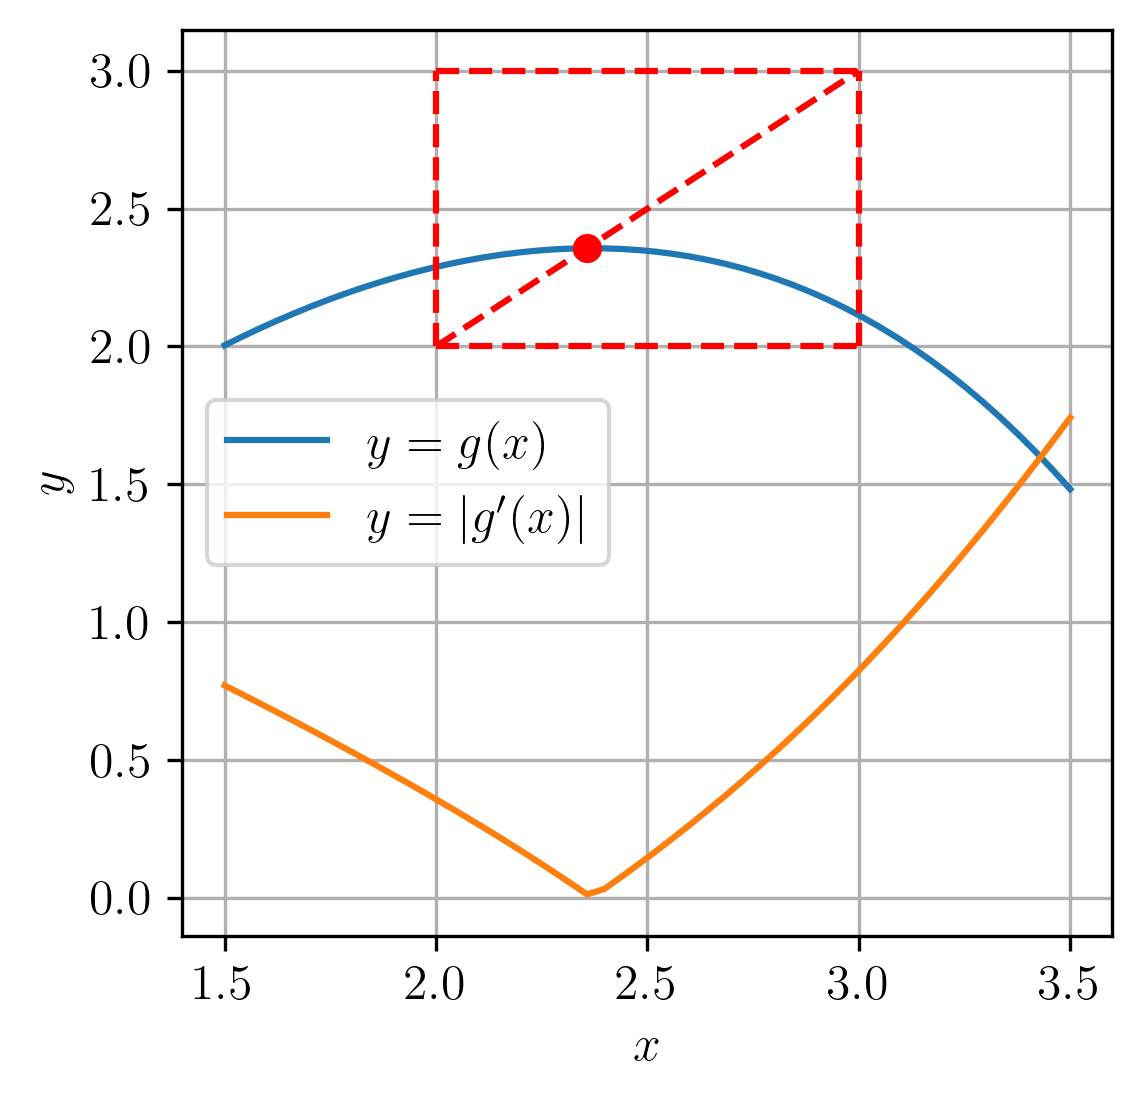
\includegraphics[width=\textwidth]{./cap_eq1d/dados/fig_ex_pfixo_exec/fig}
  \caption{Esboço dos gráficos de $g$ e $|g'|$ discutidas no Exemplo \ref{cap_eq1d_sec_pfixo:ex:pfixo_exec}.}
  \label{cap_eq1d_sec_pfixo:fig:ex_pfixo_exec}
\end{figure}

Então, fazendo as iterações de ponto fixo com aproximação inicial $x^{(0)}=2,6$, obtemos os resultados apresentados na Tabela \ref{cap_eq1d_sec_pfixo:tab:ex_pfixo_exec}.

\begin{table}[H]
  \centering
  \caption{Resultados referentes ao Exemplo \ref{cap_eq1d_sec_pfixo:ex:pfixo_exec}.}
  \label{cap_eq1d_sec_pfixo:tab:ex_pfixo_exec}
  \begin{tabular}{r|cc}
    $k$ & $x^{(k)}$ & $|x^{(k)}-x^{(k-1)}|$ \\\hline
    0 & $2,6000$ & -x-\\
    1 & $2,3264$ & $2,7\E-1$ \\
    2 & $2,3553$ & $2,9\E-2$ \\
    3 & $2,3562$ & $8,4\E-4$ \\
    4 & $2,3562$ & $1,1\E-5$ \\\hline
  \end{tabular}
\end{table}

\begin{lstlisting}
import numpy as np

# fun obj
f = lambda x: np.sin(x+np.pi/4)**2 \
  - x**3 + np.pi/4*x**2 + 5*np.pi**2/16*x \
  + 3*np.pi**3/64

# param
alpha = -0.1
# fun pto fixo
g = lambda x: x - alpha*f(x)

# aprox inicial
x0 = 2.6
print(f'\n{1}: {x0:.4f}')
for k in range(4):
  x = g(x0)
  nd = np.fabs(x-x0)
  print(f'{k+1}: {x:.4f}, {nd:.1e}')
  x0 = x
\end{lstlisting}

\end{ex}

\subsection{Exercícios}

\begin{exer}
  Forneça o(s) ponto(s) fixo(s) de
  \begin{equation}
    g(x) = x^2e^{-x^2}.
  \end{equation}
\end{exer}
\begin{resp}
  $x=0$
\end{resp}

\begin{exer}
  Verifique se a iteração de ponto fixo é convergente para as seguintes funções e aproximações iniciais:
  \begin{enumerate}[a)]
  \item $g_1(x) = \cos(x)$, $x^{(1)} = 0,5$
  \item $g_2(x) = x^2$, $x^{(1)} = 1,01$
  \end{enumerate}
  Justifique sua resposta.
\end{exer}
\begin{resp}
  a) Convergente; b) Divergente.
\end{resp}

\begin{exer}
  Considere o problema de computar uma aproximação do zero de $f(x)=x-\cos(x)$. Resolva-o aplicando a iteração de ponto fixo para a função auxiliar
  \begin{equation}
    g(x) = x - \alpha f(x),
  \end{equation}
restrita ao intervalo $[a, b] = [0.5, 1]$ com aproximação inicial $x^{(0)}=(a+b)/2$. Escolha o melhor valor de $\alpha$ entre os seguintes:
\begin{enumerate}
\item $\alpha = 1$
\item $\alpha = 0,5$
\item $\alpha = -0,5$
\item $\alpha = 0,6$
\end{enumerate}
Então, compute uma aproximação do zero de $f$ com $5$ dígitos significativos de precisão.
\end{exer}
\begin{resp}
  $\alpha=0,6$; $7,3909\times 10^{-1}$
\end{resp}

\begin{exer}
  Seja
  \begin{equation}
    \begin{aligned}
      f(x) &= \sen^2\left(x+\frac{\pi}{4}\right) - x^3\\
      &+ \frac{\pi}{4}x^2 + \frac{5\pi^2}{16}x + \frac{3\pi^3}{64}.
    \end{aligned}
\end{equation}
  \begin{enumerate}[a)]
  \item Aplique a iteração de ponto fixo na função auxiliar
    \begin{equation}
      g(x) = x - \alpha f(x)
    \end{equation}
    para algum $\alpha$ adequado, de forma que aproximação inicial $x^{(0)}=-0,5$ leve a iterações de ponto fixo que convirjam para $x^*=-\pi/4$, zero de multiplicidade par de $f$.
  \item Mostre que $g'(x^*) = 1$ para qualquer valor de $\alpha$. Por que isso explica a lenta convergência observada no item a)?
  \item Alternativamente, verifique que a abordagem da iteração de ponto fixo converge muito mais rápido para $x^*$ se aplicada à derivada de $f$, i.e. aplicando a iteração à função auxiliar
    \begin{equation}
      h(x) = x - \alpha f'(x),
    \end{equation}
    para um valor de $\alpha$ adequado.
  \end{enumerate}
\end{exer}
\begin{resp}
  a) $\alpha = 0.25$; b) Pois, não há $\alpha$ que satisfaz o Teorema do Ponto Fixo.; c) $\alpha = 0.1$
\end{resp}

\begin{exer}
  Use o Método da Iteração de Ponto Fixo para aproximar um zero de
  \begin{equation}
    f(x)=x^3\sen(x)-\cos(x)
  \end{equation}
  no intervalo inicial $[0,5, 1]$.
\end{exer}

\begin{exer}
  Use o Método da Iteração de Ponto Fixo para computar a(s) solução(ões) das seguintes equações com precisão de 8 dígitos significativos.
  \begin{enumerate}[a)]
  \item $x = 2^{-x}$ para $0\leq x \leq 2$.
  \item $e^{-x^2} = 3x - x^2$ para $-1\leq x\leq 4$.
  \end{enumerate}
\end{exer}
\begin{resp}
  a) $6.4118574\times 10^{-1}$; b) $3.3536470\times 10^{-1}$; $2.9999589$
\end{resp}

\begin{exer}
  Use o Método de Iteração de Ponto Fixo para encontrar uma aproximação com precisão de $4$ dígitos significativos do zero de 
  \begin{equation}
    \begin{aligned}
      f(x) &= (-x^2+1,154x-0,332929)\cos(x) + x^2 \\
      &- 1,154x + 0,332929
  \end{aligned}
  \end{equation}
  no intervalo $[-1, 0]$.
\end{exer}
\begin{resp}
  $-7,861\times 10^{-1}$
\end{resp}

\begin{exer}
  Use o Método de Iteração de Ponto Fixo para encontrar uma aproximação com precisão de $10^{-4}$ do zero de
  \begin{equation}
    \begin{aligned}
      f(x) &= (-x^2+1,154x-0,332929)\cos(x) + x^2\\
      &- 1,154x + 0,332929
  \end{aligned}
  \end{equation}
no intervalo $(0,55, ~0,65)$. Forneça a aproximação computada com $7$ dígitos significativos por arredondamento.
\end{exer}
\begin{resp}
  $5,770508\times 10^{-1}$
\end{resp}

\begin{exer}
  Use o Método da Iteração de Ponto Fixo para encontrar o ponto crítico\endnote{Definimos que $x$ é ponto crítico de uma dada $f$, quando $f'(x) = 0$ ou $\nexists f'(x)$.} de
  \begin{equation}
    f(x) = (1-x^2)e^{-x^2}
  \end{equation}
  no intervalo $(0, 2)$. Obtenha o resultado com precisão de $5$ dígitos significativos por arredondamento.
\end{exer}

\ifisbook
\subsubsection{Respostas}
\shipoutAnswer
\fi

%%% SECTION %%%

\section{Método de Steffensen}\label{cap_eq1d_sec_Steffensen}

O método de Steffensen\endnote{Johan Frederik Steffensen, 1873 - 1961, matemático e estatístico dinamarquês. Fonte: \href{https://pt.wikipedia.org/wiki/Johan_Frederik_Steffensen}{Wikipédia}.} é uma \hl{aplicação do método de aceleração de convergência $\Delta^2$ de Aitken}\endnote{Alexander Aitken, 1895 - 1967, matemático neozelandês. Fonte: \href{https://pt.wikipedia.org/wiki/Alexander_Aitken}{Wikipédia}.} \hl{à iteração de ponto fixo}.

\subsection{Acelerador $\Delta^2$ de Aitken}

Seja dada uma sequência $(x^{(k)})_{k=1}^\infty$ monotonicamente convergente para $x^*$. Assumimos que $k$ seja suficientemente grande tal que
\begin{equation}
  \frac{x^{(k+1)}-x^*}{x^{(k)}-x^*} \approx \frac{x^{(k+2)}-x^*}{x^{(k+1)}-x^*}.
\end{equation}
Então, isolando $x^*$ obtemos
\begin{equation}
  x^* \approx \frac{x^{(k)}x^{(k+2)}-(x^{(k+1)})^2}{x^{(k)}-2x^{(k+1)}+x^{(k+2)}}.
\end{equation}
Ainda, somando e subtraindo $(x^{(k)})^2$ e $2x^{(k)}x^{(k+1)}$ no numerador acima e rearranjando os termos, obtemos
\begin{equation}
  x^* \approx x^{(k)} - \frac{(x^{(k+1)}-x^{(k)})^2}{x^{(k+2)}-2x^{(k+1)}+x^{(k)}}.
\end{equation}

O observado acima, nos motiva a introduzir o \hl{acelerador $\Delta^2$ de Aitken}
\begin{equation}\label{cap_eq1d_sec_Steffensen:eq:ac_aitken}
  {\color{blue}\Delta^2\{x^{(k)},x^{(k+1)},x^{(k+2)}\} := x^{(k)} - \frac{(x^{(k+1)}-x^{(k)})^2}{x^{(k+2)}-2x^{(k+1)}+x^{(k)}}}.
\end{equation}


\begin{ex}\label{cap_eq1d_sec_Steffensen:ex:Aitken}
  Consideremos o problema de encontrar o zero da função
  \begin{equation}
    \begin{aligned}
      f(x) &= \sen^2\left(x+\frac{\pi}{4}\right) - x^3 \\
      &+ \frac{\pi}{4}x^2 + \frac{5\pi^2}{16}x + \frac{3\pi^3}{64}.
  \end{aligned}
  \end{equation}
  no intervalo $[2,3]$. Para tanto, podemos aplicar a iteração de ponto fixo dada por
  \begin{equation}
    \begin{aligned}
      x^{(k+1)} &= g(x^{(k)}) \\
      &:= x^{(k)} - \alpha f(x^{(k)}),\quad k=1,2,\ldots,
  \end{aligned}
  \end{equation}
com $\alpha=-0,05$ e $x^{(0)}=2,6$. Na Tabela \ref{cap_eq1d_sec_Steffensen:tab:ex_Aitken} temos os valores das iteradas $x^{(k)}$ e das correções $\Delta^2 = \Delta^2\{x^{(k)},x^{(k+1)},x^{(k+2)}\}$ de Aitken. Neste caso, a aceleração de convergência é notável.

\begin{table}[H]
  \centering
  \caption{Resultados referentes ao Exemplo \ref{cap_eq1d_sec_Steffensen:ex:Aitken}.}
  \label{cap_eq1d_sec_Steffensen:tab:ex_Aitken}
  \begin{tabular}{r|cc}
    $k$ & $x^{(k)}$ & $\Delta^2$ \\\hline
    0 & $2,6000$ & -x- \\
    1 & $2,4632$ & -x- \\
    2 & $2,4073$ & $2,3687$ \\
    3 & $2,3814$ & $2,3590$ \\
    4 & $2,3688$ & $2,3569$ \\
    5 & $2,3625$ & $2,3564$ \\
    6 & $2,3594$ & $2,3562$ \\
    7 & $2,3578$ & $2,3562$ \\\hline
  \end{tabular}
\end{table}

\begin{lstlisting}
import numpy as np

# fun obj
f = lambda x: np.sin(x+np.pi/4)**2 \
  - x**3 + np.pi/4*x**2 + 5*np.pi**2/16*x \
  + 3*np.pi**3/64

# fun pto fixo
alpha = -0.05
g = lambda x: x - alpha*f(x)

x0 = 2.6
print(f'\n1: {x0:.4f}')
for k in range(7):
  x1 = g(x0)
  x2 = g(x1)
  x = x0 - (x1-x0)**2/(x2-2*x1+x0)
  print(f'\n{k+2}: {x1:.4f}, {x:.4f}')
  x0 = x1
\end{lstlisting}

\end{ex}

\subsection{Análise Numérica}

\begin{defn}\normalfont{(Diferença Progressiva.)}
  Para uma sequência $\left(x^{(k)}\right)_{k=1}^\infty$, $\Delta x^{(k)}$ denota o \hl{\emph{operador de diferença progressiva}} e é definido por
  \begin{equation}
    \Delta x^{(k)} := x^{(k+1)} - x^{(k)}
  \end{equation}
  Potências maiores do operador são definidas recursivamente por
  \begin{equation}
    \Delta^n x^{(k)} = \Delta\left(\Delta^{n-1}x^{(k)}\right),\quad n\geq 2.
  \end{equation}
\end{defn}

Da definição acima, temos que
\begin{align}
  \Delta^2 x^{(k)} &:= \Delta\left(\delta x^{(k)}\right)\\
                   &= \Delta\left(x^{(k+1)} - x^{(k)}\right)\\
                   &= \Delta x^{(k+1)} - \Delta x^{(k)}\\
                   &= \left(x^{(k+2)} - x^{(k+1)}\right) - \left(x^{(k+1)} - x^{(k)}\right)\\
                   &= x^{(k+2)} - 2x^{(k+1)} + x^{(k)}
\end{align}
Com isso, temos que o \hl{acelerador $\Delta^2$ de Aitken} \eqref{cap_eq1d_sec_Steffensen:eq:ac_aitken} pode ser reescrito como
\begin{equation}
  {\color{blue}\Delta^2\left\{x^{(k)}, x^{(k+1)}, x^{(k+2)}\right\} := x^{(k)} - \frac{\left(\Delta x^{(k)}\right)^2}{\Delta^2 x^{(k)}}}.
\end{equation}

\begin{teo}
  \hl{Seja $\left(x^{(k)}\right)_{k=1}^\infty$ uma sequência linearmente convergente} para $x^*$ e
  \begin{equation}\label{cap_eq1d_sec_Steffensen:eq:teo_aux}
    \lim_{k\to\infty}\frac{x^{(k+1)}-x^*}{x^{(k)}-x^*} < 1.
  \end{equation}
  Então, \hl{a sequência $\Delta^2$ de Aitken} $\left(\hat{x}^{(k)}\right)_{k=1}^\infty$, com
  \begin{equation}
    \hat{x}^{(k)} := \Delta^2\left\{x^{(k)}, x^{(k+1)}, x^{(k+2)}\right\},
  \end{equation}
  \hl{converge} para $x^*$ \hl{mais rápido que $\left(x^{(k)}\right)$} no sentido de que
  \begin{equation}
    \lim_{k\to\infty}\frac{\hat{x}^{(k)}-x^*}{x^{(k)}-x^*} = 0.
  \end{equation}
\end{teo}
\begin{dem}
  \emconstrucao
\end{dem}

\subsection{Algoritmo de Steffensen}

O método de Steffensen \hl{consiste em aplicar o acelerador $\Delta^2$ de Aitken à iteração de ponto fixo}. Mais especificamente, sejam uma aproximação inicial $x^{(0)}$ e uma iteração de ponto fixo
\begin{equation}
  x^{(k+1)} = g(x^{(k)}),\quad k=0, 1, 2, \ldots.
\end{equation}
O algoritmo de Steffensen consiste em:
\begin{enumerate}
\item $x \leftarrow x^{(0)}$.
\item Para $k=0, 1, 2, \dotsc, N-1$:
  \begin{enumerate}
  \item $x_1 \leftarrow g(x)$.
  \item $x_2 \leftarrow g(x_1)$.
  \item $x^{(k+1)} \leftarrow \Delta^2\{x,x_1,x_2\}$.
  \item $x \leftarrow x^{(k+1)}$.
  \end{enumerate}
\end{enumerate}


\begin{ex}\label{cap_eq1d_sec_Steffensen:ex:Steffensen_exec}
  Retornamos ao exemplo anterior (Exemplo \ref{cap_eq1d_sec_Steffensen:ex:Aitken}. Na Tabela \ref{cap_eq1d_sec_Steffensen:tab:ex_Steffensen_exec} temos os valores das iteradas de Steffensen $x^{(k)}$ e do indicador de convergência $|x^{(k)}-x^{(k-1)}|$.

\begin{table}[h!]
  \centering
  \caption{Resultados referentes ao Exemplo \ref{cap_eq1d_sec_Steffensen:ex:Steffensen_exec}.}
  \label{cap_eq1d_sec_Steffensen:tab:ex_Steffensen_exec}
  \begin{tabular}{r|cc}
    $k$ & $x^{(k)}$ & $|x^{(k)}-x^{(k-1)}|$ \\\hline
    0 & $2,6000$ & -x- \\
    1 & $2,3687$ & $2,3\E-1$ \\
    2 & $2.3562$ & $1,2\E-2$ \\
    3 & $2,3562$ & $4,2\E-5$ \\\hline
  \end{tabular}
\end{table}

\begin{lstlisting}
import numpy as np

# fun obj
f = lambda x: np.sin(x+np.pi/4)**2 \
  - x**3 + np.pi/4*x**2 + 5*np.pi**2/16*x \
  + 3*np.pi**3/64

# fun pto fixo
alpha = -0.05
g = lambda x: x - alpha*f(x)

x0 = 2.6
print(f'\n1: {x0:.4f}')
for k in range(3):
  x1 = g(x0)
  x2 = g(x1)
  x = x0 - (x1-x0)**2/(x2-2*x1+x0)
  nd = np.fabs(x-x0)
  print(f'\n{k+2}: {x:.4f}, {nd:.1e}')
  x0 = x
\end{lstlisting}

\end{ex}

\subsection*{Exercícios}

\begin{exer}
  Use o método de Steffensen para obter uma aproximação do zero de $f(x)=x^3\sen(x)-\cos(x)$ no intervalo $[0,5, 1]$ com precisão de $10^{-6}$.
\end{exer}
\begin{resp}
    $9,15811\times 10^{-1}$
\end{resp}

\begin{exer}
  Use o Método da Iteração de Ponto Fixo para aproximar um zero de
  \begin{equation}
    f(x)=x^3\sen(x)-\cos(x)
  \end{equation}
  no intervalo inicial $[0,5, 1]$.
\end{exer}

\begin{exer}
  Use o Método de Steffensen para computar a(s) solução(ões) das seguintes equações com precisão de 8 dígitos significativos.
  \begin{enumerate}[a)]
  \item $x = 2^{-x}$ para $0\leq x \leq 2$.
  \item $e^{-x^2} = 3x - x^2$ para $-1\leq x\leq 4$.
  \end{enumerate}
\end{exer}
\begin{resp}
  a) $6.4118574\times 10^{-1}$; b) $3.3536470\times 10^{-1}$; $2.9999589$
\end{resp}

\begin{exer}
  Use o Método de Steffensen para encontrar uma aproximação com precisão de $4$ dígitos significativos do zero de 
  \begin{equation}
    f(x) = (-x^2+1,154x-0,332929)\cos(x) + x^2 - 1,154x + 0,332929
  \end{equation}
  no intervalo $[-1, 0]$.
\end{exer}
\begin{resp}
  $-7,861\times 10^{-1}$
\end{resp}

\begin{exer}
  Use o Método de Steffensen para encontrar uma aproximação com precisão de $10^{-4}$ do zero de
  \begin{equation}
    \begin{aligned}
      f(x) &= (-x^2+1,154x-0,332929)\cos(x) + x^2 \\
      &- 1,154x + 0,332929
  \end{aligned}
  \end{equation}
no intervalo $(0,55, ~0,65)$. Forneça a aproximação computada com $7$ dígitos significativos por arredondamento.
\end{exer}
\begin{resp}
  $5,770508\times 10^{-1}$
\end{resp}

\begin{exer}
  Use o Método de Steffensen para encontrar o ponto crítico\endnote{Definimos que $x$ é ponto crítico de uma dada $f$, quando $f'(x) = 0$ ou $\nexists f'(x)$.} de
  \begin{equation}
    f(x) = (1-x^2)e^{-x^2}
  \end{equation}
  no intervalo $(0, 2)$. Obtenha o resultado com precisão de $5$ dígitos significativos por arredondamento.
\end{exer}

\ifisbook
\subsubsection{Respostas}
\shipoutAnswer
\fi

%%% SECTION %%%

\section{Método de Newton}\label{cap_eq1d_sec_newton}

Seja $x^*$ um zero de uma dada função $f$, i.e.
\begin{equation}
  f(x^*)=0.
\end{equation}
A expansão em polinômio de Taylor{\taylor} de $f$ em um ponto $\tilde{x}$ dado, é
\begin{equation}
  f(x^*) = f(\tilde{x}) + f'(\tilde{x})(x^*-\tilde{x}) + O\left(\left|x^*-\tilde{x}\right|^2\right).
\end{equation}
Como $f(x^*)=0$, temos
\begin{align}
  & 0 = f(\tilde{x}) + f'(\tilde{x})(x^*-\tilde{x}) + O\left(\left|x^*-\tilde{x}\right|^2\right)\\
  & x^* = \tilde{x} - \frac{f(\tilde{x})}{f'(\tilde{x})} + O\left(\left|x^*-\tilde{x}\right|^2\right)
\end{align}
Esta última expressão nos indica que \hl{dada uma aproximação $\tilde{x}$ do zero de $f$ a expressão}
\begin{equation}
  \hleq{\tilde{x} - \frac{f(\tilde{x})}{f'(\tilde{x})}},
\end{equation}
\hl{aproxima $x^*$ com um erro da ordem de $|x^*-\tilde{x}|^2$}.

Estas observações nos levam a \hl{\emph{iteração de Newton}}\endnote{Sir Isaac Newton, matemático e físico inglês, 1642 - 1726/27. Fonte: \href{https://en.wikipedia.org/wiki/Isaac_Newton}{Wikipedia}.}\index{iteração de!Newton}
\begin{align}
  \hleq{x^{(0)}} &\hleq{= \text{aprox. inicial}},\\
  \hleq{x^{(k+1)}} &\hleq{= x^{(k)} - \frac{f(x^{(k)})}{f'(x^{(k)})}},\label{cap_eq1d_sec_newton:eq:Newton_iteracao}
\end{align}
com $k=0, 1, 2, \ldots$.

\begin{ex}\label{cap_eq1d_sec_newton:ex:newton}
  Consideramos o problema de encontrar o zero da função
  \begin{equation}
    \begin{aligned}
      f(x) &= \sen^2\left(x+\frac{\pi}{4}\right) - x^3 \\
      &+ \frac{\pi}{4}x^2 + \frac{5\pi^2}{16}x + \frac{3\pi^3}{64}.
    \end{aligned}
  \end{equation}
  no intervalo $[2,3]$ (Consulte a Figura~\ref{cap_eq1d_sec_newton:fig:newton_ex}).

  \begin{figure}[H]
    \centering
    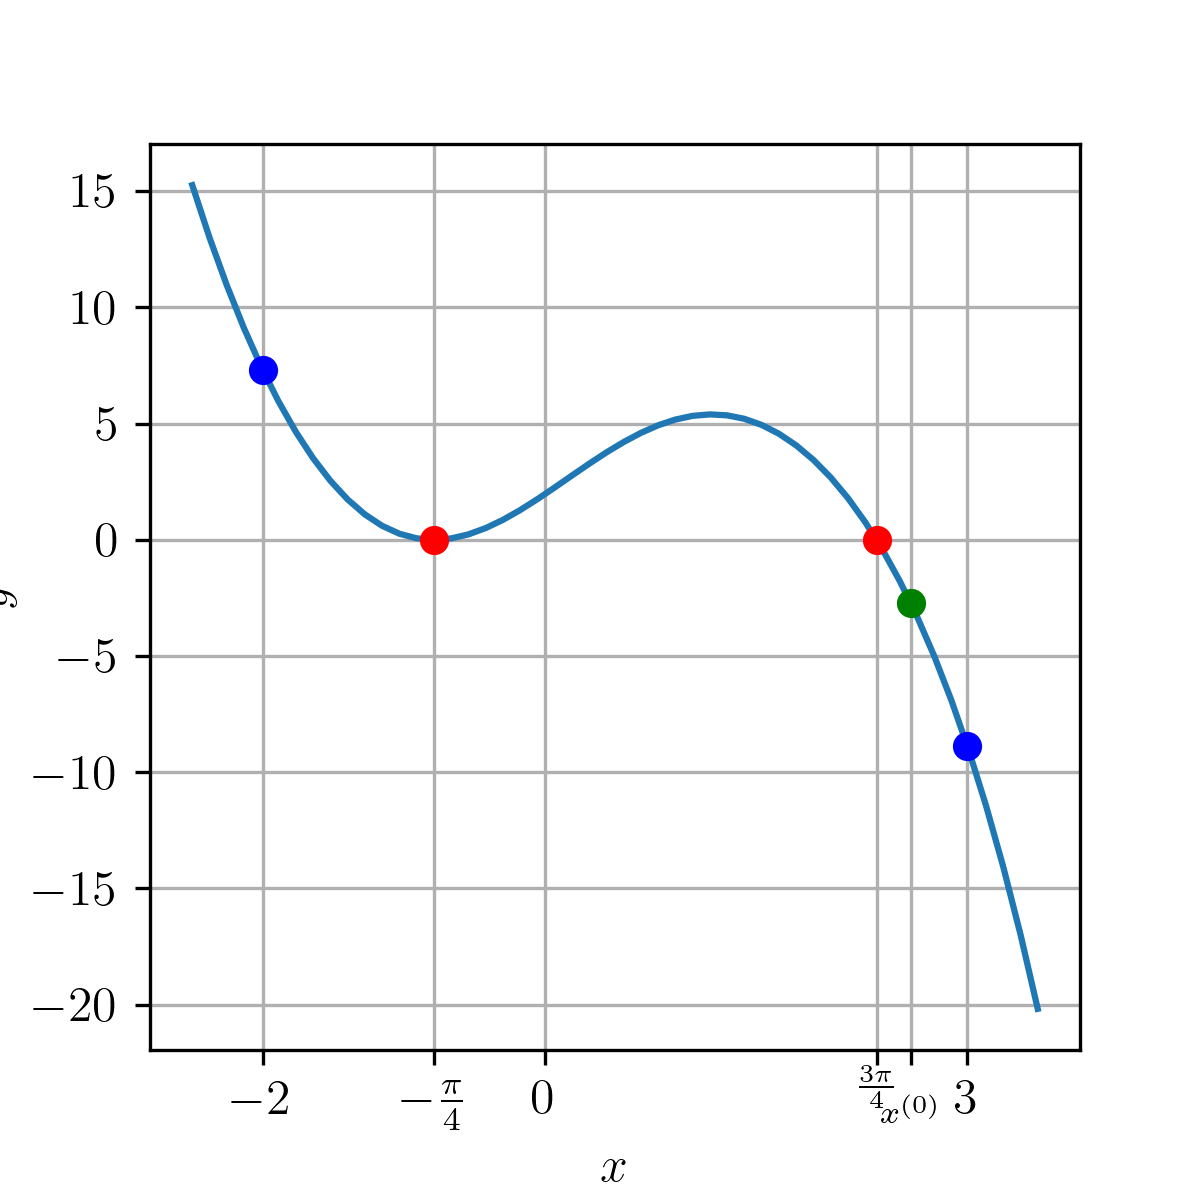
\includegraphics[width=0.8\textwidth]{./cap_eq1d/dados/fig_newton_ex/fig}
    \caption{Esboço da função $f$ do Exemplo~\ref{cap_eq1d_sec_newton:ex:newton}.}
  \label{cap_eq1d_sec_newton:fig:newton_ex}
\end{figure}


  Fazendo as iterações de Newton com aproximação inicial $x^{(0)}=2,6$, obtemos os resultados apresentados na Tabela \ref{tab:ex_Newton_exec}.

  \begin{table}[h!]
    \centering
    \caption{Resultados referentes ao Exemplo~\ref{cap_eq1d_sec_newton:ex:newton}.}
    \label{tab:ex_Newton_exec}
    \begin{tabular}{r|cc}
      $k$ & $x^{(k)}$ & $|x^{(k)}-x^{(k-1)}|$ \\\hline
      0 & $2,6000$ & -x-\\
      1 & $2,3836$ & $2,2\E-1$ \\
      2 & $2,3566$ & $2,7\E-2$ \\
      3 & $2,3562$ & $3,9\E-4$ \\
      4 & $2,3562$ & $8,3\E-8$ \\\hline
    \end{tabular}
  \end{table}

\begin{lstlisting}
import numpy as np

# fun obj
f = lambda x: np.sin(x+np.pi/4)**2 \
  - x**3 + np.pi/4*x**2 + 5*np.pi**2/16*x \
  + 3*np.pi**3/64

fl = lambda x: 2*np.sin(x+np.pi/4)*np.cos(x+np.pi/4) \
  -3*x**2 + np.pi/2*x + 5*np.pi**2/16

# aprox. inicial
x0 = 2.6
print(f'0: {x0:.4e}')

# iterações
for k in range(4):
  x = x0 - f(x0)/fl(x0)
  print(f'{k+1}: {x:.4e}')
  x0 = x
\end{lstlisting}

\end{ex}

\begin{obs}
  \hl{O método de Newton é uma iteração de ponto fixo ótima}. Do Teorema do Ponto Fixo (Teorema~\ref{cap_eq1d_sec_pfixo:teo:pfixo}), a iteração
  \begin{align}
    x^{k+1} &= g(x^{(k)})\\
            &:= x^{(k)} -\alpha f(x)\label{cap_eq1d_sec_pfixo:eq:Newton_pfixo}
  \end{align}
tem taxa de convergência\endnote{Supondo verdadeiras as demais hipóteses do Teorema~\ref{cap_eq1d_sec_pfixo:teo:pfixo}.}
\begin{equation}
  |x^{(k+1)}-x^{(k)}| \leq K |x^{(k)}-x^{(k-1)}|,
\end{equation}
com $K$ tal que $|g'(x)| = |1 - \alpha f'(x)| < K < 1$. Isto nos indica que a melhor escolha para $\alpha$ é
\begin{equation}
  \alpha = \frac{1}{f'(x)},
\end{equation}
de forma que \eqref{cap_eq1d_sec_pfixo:eq:Newton_pfixo} coincide com a iteração de \eqref{cap_eq1d_sec_newton:eq:Newton_iteracao}.
\end{obs}

\subsection{Interpretação Geométrica}

Dadas uma aproximação $x^{(k)}$ de um zero de uma função $f$, a iteração de Newton fornece uma nova aproximação $x^{(k+1)}$ com
\begin{equation}
  x^{(k+1)} = x^{(k)} - \frac{f(x^{(k)})}{f'(x^{(k)})}.
\end{equation}
Subtraindo $x^{(k+1)}$ e multiplicando por $-f'(x^{(k)})$, obtemos
\begin{equation}\label{cap_eq1d_sec_newton:eq:Newton_geointerp}
  0 = f'(x^{(k)})(x^{(k+1)}-x^{(k)}) + f(x^{(k)}),
\end{equation}
Observemos que o lado direito desta última equação corresponde a expressão da reta tangente ao gráfico de $f$ pelo ponto $(x^{(k)}, f(x^{(k)}))$, avaliada em $x^{(k+1)}$. Mais precisamente, a equação desta reta tangente é
\begin{equation}
  y = f'(x^{(k)})(x-x^{(k)}) + f(x^{(k)})
\end{equation}
e a equação \eqref{cap_eq1d_sec_newton:eq:Newton_geointerp} nos informa que em $x=x^{(k+1)}$ a reta tangente cruza o eixo $x$.

\begin{figure}[H]
  \centering
  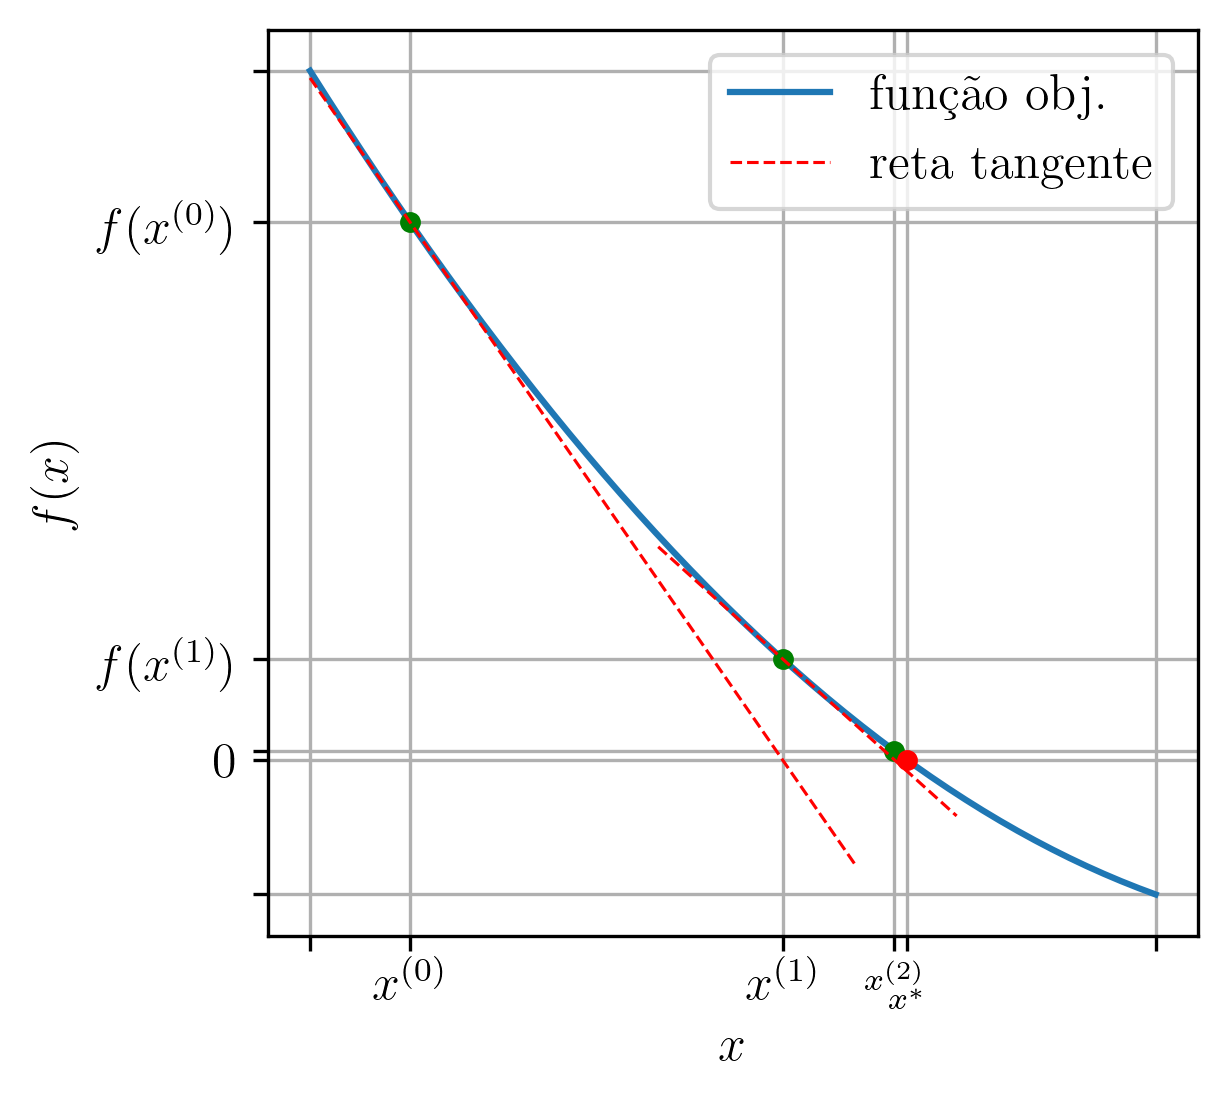
\includegraphics[width=\textwidth]{./cap_eq1d/dados/fig_Newton_geointerp/fig}
  \caption{Interpretação geométrica das iterações de Newton.}
  \label{cap_eq1d_sec_newton:fig:Newton_geointerp}
\end{figure}

Destas observações, concluímos que \hl{a iterada $x^{(k+1)}$ do método de Newton corresponde ao ponto de interseção da reta tangente ao gráfico da $f$ pelo ponto $(x^{k}, f(x^{k}))$ com o eixo das abscissas}\endnote{Eixo $x$.}. Consulte a Figura~\ref{cap_eq1d_sec_newton:fig:Newton_geointerp}.

\begin{ex}\label{cap_eq1d_sec_newton:ex:Newton_init}
  Consideremos que o método de Newton seja usado para aproximarmos o zero de
  \begin{equation}
    f(x) = (x-1)e^{-x^2}.
  \end{equation}
Observemos que esta função tem $x=1$ como seu único zero. Agora, se escolhermos $x^{(0)} = 0,5$ as iterações de Newton convergem para este zero, mas, se escolhermos $\tilde{x}^{(0)}=1,5$ não (consulte a Tabela~\ref{cap_eq1d_sec_newton:tab:ex_Newton_init}).

\begin{table}[H]
  \centering
  \caption{Resultados referentes ao Exemplo \ref{cap_eq1d_sec_newton:ex:Newton_init}}
  \label{cap_eq1d_sec_newton:tab:ex_Newton_init}
  \begin{tabular}{r|cc}
    $k$ & $x^{(k)}$   & $\tilde{x}^{(k)}$ \\\hline
    0 & $5,0000\E-1$ & $1,5000\E+0$ \\
    1 & $8,3333\E-1$ & $2,5000\E+0$ \\
    2 & $9,6377\E-1$ & $2,7308\E+0$ \\
    3 & $9,9763\E-1$ & $2,9355\E+0$ \\
    4 & $9,9999\E-1$ & $3,1223\E+0$ \\
    5 & $1,0000\E+0$ & $3,2955\E+0$ \\
  \end{tabular}
\end{table}

\begin{figure}[H]
  \centering
  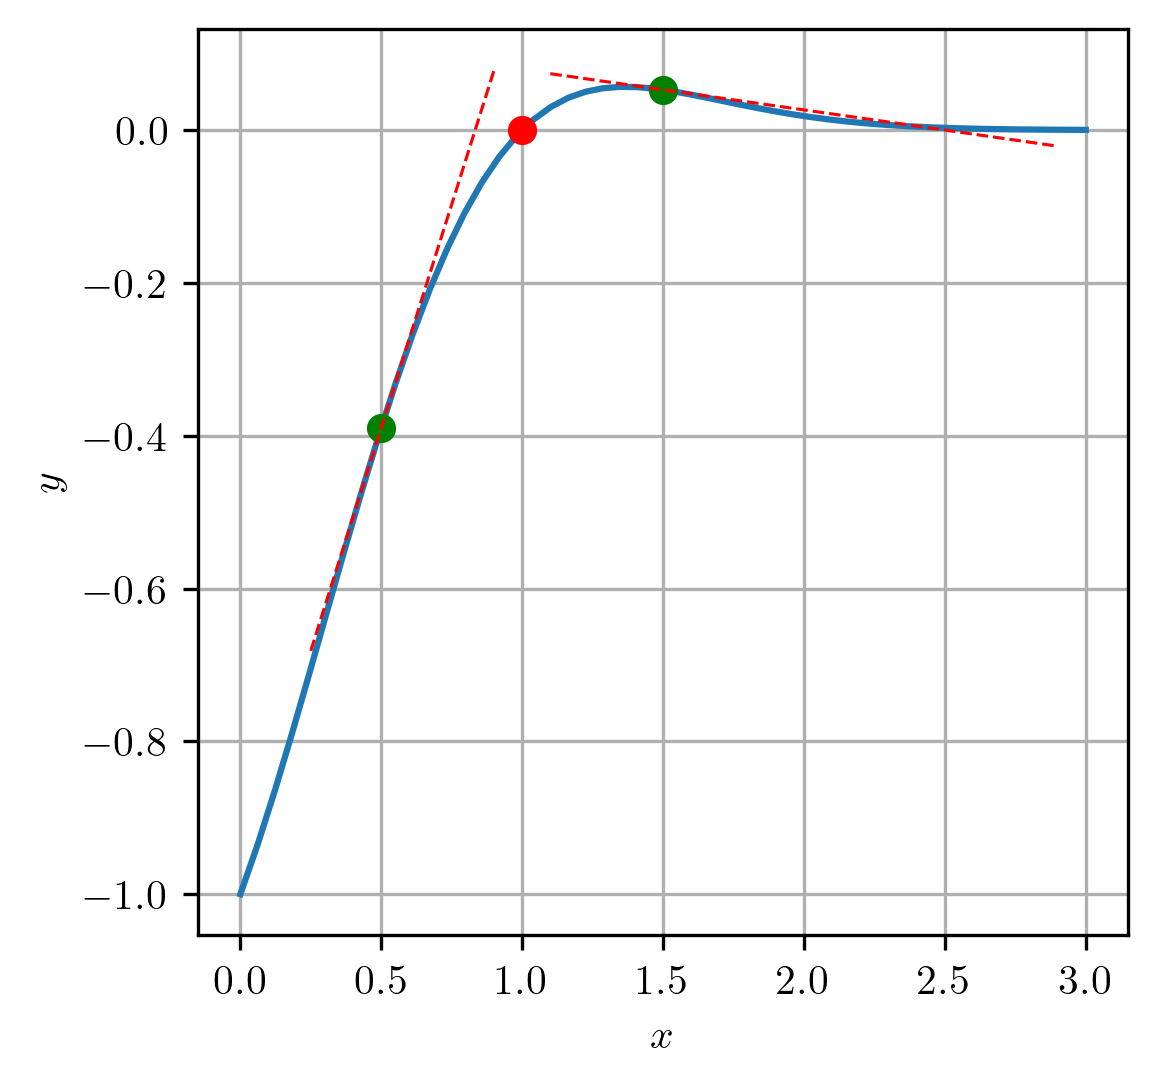
\includegraphics[width=\textwidth]{./cap_eq1d/dados/fig_newton_ex_init/fig}
  \caption{Escolha da aproximação inicial para o método de Newton.}
  \label{cap_eq1d_sec_newton:fig:ex_Newton_init}
\end{figure}

Embora ambas aproximações iniciais estão a mesma distância da solução $x=1$, quando tomamos $x^{(0)}=1,5$ as iterações irão divergir, como podemos observar da interpretação geométrica dada na Figura \ref{cap_eq1d_sec_newton:fig:ex_Newton_init}.
\end{ex}

\subsection{Análise de Convergência}

Seja $x^*$ o zero de uma dada função \hl{$f$ duas vezes continuamente diferenciável com $f'(x)\neq 0$} para todo $x\in [x^*-\varepsilon_0, x^*+\varepsilon_0]$ para algum $\varepsilon_0>0$. Seja, também, $(x^{(k)})_{k=0}^\infty$ a sequência das iteradas de Newton
\begin{equation}\label{eq:newton_iter1}
  x^{(k+1)} = x^{(k)} - \frac{f(x^{(k)})}{f'(x^{(k)})},\quad k=0, 1, 2, \ldots,
\end{equation}
com aproximação inicial $x^{(0)}\in (x^*-\varepsilon_0, x^*+\varepsilon_0)$. Então, do polinômio de Taylor de grau 1 de $f$ em torno de $x^{(0)}$, temos
\begin{equation}
  f(x^*) = f(x^{(0)}) + f'(x^{(0)})(x^* - x^{(0)}) + \frac{f''(\xi^{(0)})}{2!}(x^*-x^{(0)})^2,
\end{equation}
onde $\xi^{(0)}$ está entre $x^{(0)}$ e $\xi^{(0)}$. Daí, rearranjamos os termos e notamos que $f(x^*)=0$ para obtermos
\begin{equation}
  x^* - \left[x^{(0)} - \frac{f(x^{(0)})}{f'(x^{(0)})}\right] = \frac{f''(\xi^{(0)})}{2f'(x^{(0)})}(x^*-x^{(0)})^2.
\end{equation}
Então, da iteração de Newton \eqref{eq:newton_iter1}, temos
\begin{equation}
  x^* - x^{(1)} = \frac{f''(\xi^{(0)})}{2f'(x^{(0)})}(x^* - x^{(0)})^2
\end{equation}
Logo,
\begin{equation}\label{eq:newton_taxa_1}
  |x^* - x^{(1)}| \leq C |x^* - x^{(0)}|^2,
\end{equation}
com
\begin{equation}
  C = \sup_{x,y\in [x^*-\varepsilon, x^*+\varepsilon]} \left|\frac{f''(x)}{2f'(y)}\right|.
\end{equation}
Segue, então, que se $x^{(0)}\in (x^*-\varepsilon, x^* + \varepsilon)$ para algum $\varepsilon>0$ tal que
\begin{equation}
  C |x^* - x^{(0)}|^2 < 1,\quad\forall x\in (x^*-\varepsilon, x^* + \varepsilon),
\end{equation}
então $x^{(1)}\in (x^*-\varepsilon, x^*+\varepsilon)$.

Logo, por indução matemática\endnote{Veja o exercício \ref{ex:Newton_analise_conv}.}, temos que \hl{o método de Newton tem ordem de convergência quadrática}
\begin{equation}\label{eq:Newton_taxa_quadratica}
  \hleq{|x^{(k+1)}-x^*| \leq C|x^{(k)}-x^{*}|^{\pmb{2}}},
\end{equation}
\hl{para qualquer escolha de $x^{(0)}$ suficientemente próximo de $x^*$}, i.e. $x^{(0)}\in (x^*-\varepsilon, x^*+\varepsilon)$.

\begin{obs}
  O intervalo $(x^*-\varepsilon, x^*+\varepsilon)$ é chamado de \hl{\emph{bacia de atração} do método de Newton}.
\end{obs}

\begin{ex}\label{ex:Newton_taxa}
  Retornamos ao problema de encontrar o zero da função
  \begin{equation}
    \begin{aligned}
      f(x) &= \sen^2\left(x+\frac{\pi}{4}\right) - x^3 \\
      &+ \frac{\pi}{4}x^2 + \frac{5\pi^2}{16}x + \frac{3\pi^3}{64}.
  \end{aligned}
  \end{equation}
  no intervalo $[2,3]$. Este problema foi construído de forma que $x^* = 3\pi/4$ é um zero de $f$. Então, fazendo as iterações de Newton com aproximação inicial $x^{(0)}=2,6$, obtemos os resultados apresentados na Tabela \ref{tab:ex_Newton_taxa}, os quais evidenciam a convergência quadrática das iterações computadas.

\begin{table}[h!]
  \centering
  \caption{Resultados referentes ao Exemplo \ref{ex:Newton_taxa}.}
  \label{tab:ex_Newton_taxa}
  \begin{tabular}{r|cc}
    $k$ & $x^{(k)}$ & $|x^{(k)}-x^*|$ \\\hline
    0 & $2,6000$ & $2,4\E-01$ \\
    1 & $2,3836$ & $2,7\E-02$ \\
    2 & $2,3566$ & $3,9\E-04$ \\
    3 & $2,3562$ & $8,3\E-08$ \\
    4 & $2,3562$ & $3,6\E-15$ \\\hline
  \end{tabular}
\end{table}

\end{ex}

\subsection{Zeros Múltiplos}\index{zeros múltiplos}

Na análise de convergência acima foi necessário assumir que $f'(x) \neq 0$ para todo $x$ em uma vizinha do zero $x^*$ da função $f$. Isto não é possível no caso de $x^*$ ser um zero duplo pois, então, $f'(x^*) = 0$. Neste caso, podemos aplicar o método de Newton a $f'(x)$, a qual tem $x^*$ como um zero simples.

\begin{ex}\label{ex:Newton_multpar}
  Consideremos o problema de aproximar o zero da função
  \begin{equation}\label{cap_eq1d_sec_newton:eq:funex}
    \begin{aligned}
      f(x) &= \sen^2\left(x+\frac{\pi}{4}\right) - x^3 \\
      &+ \frac{\pi}{4}x^2 + \frac{5\pi^2}{16}x + \frac{3\pi^3}{64}.
  \end{aligned}
  \end{equation}
  no intervalo $[-1,0]$. Este problema foi construído de forma que $x^* = -\pi/4$ é um zero duplo de $f$. Então, aplicamos o método de Newton a
  \begin{equation}
    \begin{aligned}
      f'(x) &= 2\sen\left(x+\frac{\pi}{4}\right)\cos\left(x+\frac{\pi}{4}\right) \\
      &- 3x² + \frac{\pi}{2}x+\frac{5\pi^2}{16}.
  \end{aligned}
  \end{equation}
Ou seja, as iterações de Newton são
\begin{equation}
  x^{(k+1)} = x^{(k)} - \frac{f'(x^{(k)})}{f''(x^{(k)})},\quad k=0, 1, 2, \ldots,
\end{equation}
sendo $x^{(1)}$ uma aproximação inicial. Na Tabela~\ref{cap_eq1d_sec_newton:tab:ex_Newton_multpar}, temos os resultados obtidos da computação destas iterações com $x^{(1)}=-0,5$.

\begin{table}[h!]
  \centering
  \caption{Resultados referentes ao Exemplo \ref{cap_eq1d_sec_newton:ex:Newton_multpar}.}
  \label{cap_eq1d_sec_newton:tab:ex_Newton_multpar}
  \begin{tabular}{r|cc}
    $k$ & $x^{(k)}$ & $|x^{(k)}-x^*|$ \\\hline
    0 & -0.5000 & \\
    1 & -0.8341 & 3.3e-01\\
    2 & -0.7862 & 4.8e-02\\
    3 & -0.7854 & 7.9e-04\\
    4 & -0.7854 & 2.3e-07\\
    5 & -0.7854 & 1.9e-14\\\hline
  \end{tabular}
\end{table}

\end{ex}

\begin{obs}\normalfont{\hl{(Zeros múltiplos.)}}\label{cap_eq1d_sec_newton:obs:zeros_multiplos}
  No caso de zeros de multiplicidade $m>1$ de uma dada função $f$, podemos aplicar o método de Newton à derivada $m-1$ de $f$, o que requer o cálculo de $m$ derivadas de $f$. Alternativamente, consideramos aplicar o método à função auxiliar
  \begin{equation}
    \hleq\mu(x) := \frac{f(x)}{f'(x)}.
  \end{equation}
  De fato, se $x^*$ é zero de multiplicidade $m\geq 1$ de $f$, então existe uma função $g$ tal que $g(x^*)\neq 0$ e
  \begin{equation}
    f(x) = \left(x-x^*\right)^mg(x)
  \end{equation}
  Com isso, temos
  \begin{align*}
    \mu(x) &= \frac{\left(x-x^*\right)^mg(x)}{m\left(x-x^*\right)^{m-1}g(x)+\left(x-x^*\right)^mg'(x)}\\
           &= \frac{\left(x-x^*\right)g(x)}{mg(x) + \left(x-x^*\right)g'(x)}
  \end{align*}
  Como $g\left(x^*\right)\neq 0$, temos que
  \begin{equation}
    \frac{g(x^*)}{mg\left(x^*\right) + \left(x^*-x^*\right)g'\left(x^*\right)} = \frac{1}{m}\neq 0.
  \end{equation}
  Ou seja, $x^*$ é um zero simples de $\mu$. A iteração do Método de Newton aplicado à $\mu$ fornece
  \begin{align}
    x^{(k+1)} &= x^{(k)} - \frac{\mu\left(x^{(k)}\right)}{\mu'\left(x^{k+1}\right)}\\
              &= x^{(k)} = \frac{\frac{f\left(x^{(k)}\right)}{f'\left(x^{(k)}\right)}}{\frac{\left[f'\left(x^{(k)}\right)\right]^2 - f\left(x^{(k)}\right)f''\left(x^{(k)}\right)}{\left[f'\left(x^{(k)}\right)\right]^2}}
  \end{align}
  Rearranjando os termos, obtemos a \hl{iteração modificada de Newton para zeros de multiplicidade maior que 1}
  \begin{equation}\label{cap_eq1d_sec_newton:eq:iter_newton_zero_multiplo}
    \hleq x^{(k+1)} = x^{(k)} - \frac{f\left(x^{(k)}\right)f'\left(x^{(k)}\right)}{\left[f'\left(x^{(k)}\right)\right]^2 - f\left(x^{(k)}\right)f''\left(x^{(k)}\right)}.
  \end{equation}
  Para uma aplicação, consulte o exercício \ref{cap_eq1d_sec_newton:exer:iter_newton_zeros_multiplos}.
\end{obs}

\subsection*{Exercícios}

\begin{exer}\label{exer:Newton_1}
  Use o método de Newton para obter uma aproximação do zero de $f(x)=x^3\sen(x)-\cos(x)$ no intervalo $[0,5, 1]$ com precisão de $10^{-6}$.
\end{exer}
\begin{resp}
  $9,15811\times 10^{-1}$
\end{resp}

\begin{exer}\label{exer:Newton_multpar}
  Use o método de Newton para obter uma aproximação do zero de
  \begin{equation}
    \begin{aligned}
      f(x) &= (-x^2+1,154x-0,332929)\cos(x) \\
           &+ x^2 - 1,154x + 0,332929
    \end{aligned}
\end{equation}
no intervalo $(0,55, ~0,65)$ com precisão de $10^{-5}$.
\end{exer}
\begin{resp}
  $5,7700\times 10^{-1}$
\end{resp}

\begin{exer}\label{cap_eq1d_sec_newton:exer:iter_newton_zeros_multiplos}
  A função \eqref{cap_eq1d_sec_newton:eq:funex} tem um zero de multiplicidade par em $x=-\pi/4$. Assumindo a aproximação inicial $x^{(0)} = -0,5$, aplique a iteração modificada de Newton dada em \eqref{cap_eq1d_sec_newton:eq:iter_newton_zero_multiplo} e compare os resultados com apresentados na Tabela~\ref{cap_eq1d_sec_newton:tab:ex_Newton_multpar}.
\end{exer}

\begin{exer}
  Assumindo a aproximação inicial $x^{(0)} = 1$, aproxime o zero de
  \begin{equation}
    f(x) = e^x - x - 1
  \end{equation}
  usando:
  \begin{enumerate}[a)]
  \item[a)] a iteração de Newton para $f$.
  \item[b)] a iteração de Newton para $f'$.
  \item[c)] a iteração modificada de Newton\endnote{Equação~\eqref{cap_eq1d_sec_newton:eq:iter_newton_zero_multiplo}.} para $f$.
  \end{enumerate}
  Qual a melhor abordagem? Justifique sua resposta.
\end{exer}
\begin{resp}
  Dica: Analise a convergência das iteradas para cada abordagem.
\end{resp}

\begin{exer}
  Use o Método de Newton para obter a aproximação do zero de
  \begin{equation}
    p(x) = x^3 - 3\pi x^2 + 3\pi^2 x - \pi^3.
  \end{equation}
\end{exer}
\begin{resp}
  Dica: $x=\pi$ é zero de multiplicidade 3.
\end{resp}

\subsubsection{Análise Numérica}

\begin{exer}\label{ex:Newton_analise_conv}
  Complete a demonstração por indução matemática de que o método de Newton tem taxa de convergência quadrática.
\end{exer}

\ifisbook
\subsubsection{Respostas}
\shipoutAnswer
\fi

%%% SECTION %%%

\section{Método da Secante}\label{cap_eq1d_sec_secante}

\hl{O Método da Secante é um método tipo de Newton}. Observamos que para duas aproximações $x^{(k)}$ e $x^{(k-1)}$ suficientemente próximas, temos\endnote{Razão fundamental do Cálculo.}
\begin{equation}
  f'(x^{(k)}) \approx \frac{f(x^{(k)})-f(x^{(k-1)})}{x^{(k)}-x^{(k-1)}}.
\end{equation}
Assim sendo, substituindo esta aproximação na iteração de Newton (Eq. \eqref{cap_eq1d_sec_newton:eq:Newton_iteracao}), obtemos a \hl{\emph{iteração do Método da Secante}}
\begin{subequations}\label{cap_eq1d_sec_secante:eq:iter_secante}\hleq
  \begin{align}
    x^{(0)}&, x^{(1)} = \text{aprox. iniciais},\\
    x^{(k+1)} &= x^{(k)} - f(x^{(k)})\frac{x^{(k)}-x^{(k-1)}}{f(x^{(k)})-f(x^{(k-1)})},
  \end{align}
\end{subequations}
para $k=1, 2, 3, \ldots$.

\begin{ex}\label{ex:secante_exec}
  Consideramos o problema de encontrar o zero da função
  \begin{equation}
    \begin{aligned}
      f(x) &= \sen^2\left(x+\frac{\pi}{4}\right) - x^3 \\
      &+ \frac{\pi}{4}x^2 + \frac{5\pi^2}{16}x + \frac{3\pi^3}{64}.
    \end{aligned}
  \end{equation}
  no intervalo $[2,3]$. Fazendo as iterações do Método da Secante com aproximações iniciais $x^{(0)}=2,6$ e $x^{(1)}=2,5$, obtemos os resultados apresentados na Tabela \ref{cap_eq1d_sec_secante:tab:ex_secante_exec}.

\begin{table}[h!]
  \centering
  \caption{Resultados referentes ao Exemplo \ref{cap_eq1d_sec_secante:ex:secante_exec}.}
  \label{cap_eq1d_sec_secante:tab:ex_secante_exec}
  \begin{tabular}{r|ccc}
    $k$ & $x^{(k-1)}$ & $x^{(k)}$ & $|x^{(k)}-x^{(k-1)}|$ \\\hline
    0 & $2,6000$ & $2,5000$ & -x-\\
    1 & $2,5000$ & $2.3728$ & $1,3\E-1$ \\
    2 & $2,3728$ & $2,3574$ & $1,5\E-2$ \\
    3 & $2,3574$ & $2,3562$ & $1,2\E-3$ \\
    4 & $2,3562$ & $2,3562$ & $1,1\E-5$ \\
    5 & $2,3562$ & $2,3562$ & $7,0\E-9$ \\\hline
  \end{tabular}
\end{table}

\begin{lstlisting}
import numpy as np

# fun obj
f = lambda x: np.sin(x+np.pi/4)**2 \
  - x**3 + np.pi/4*x**2 + 5*np.pi**2/16*x \
  + 3*np.pi**3/64

# aprox. iniciais
x0 = 2.6
x1 = 2.5
print(f'\n0: {x0:.4f}, {x1:.4f}')

# iterações
for k in range(5):
  x = x1 - f(x1)*(x1-x0)/(f(x1)-f(x0))
  x0 = x1
  x1 = x
  print(f'{k+1}: {x0:.4f}, {x1:.4f}, {np.fabs(x1-x0):.1e}')
\end{lstlisting}

\end{ex}

\subsection{Interpretação Geométrica}

A iteração do Método da Secante é
\begin{equation}
  x^{(k+1)} = x^{(k)} - f(x^{(k)})\frac{x^{(k)}-x^{(k-1)}}{f(x^{(k)})-f(x^{(k-1)})},
\end{equation}
donde segue que
\begin{equation}
  0 = x^{(k+1)}-x^{(k)} + f(x^{(k)})\frac{x^{(k)}-x^{(k-1)}}{f(x^{(k)})-f(x^{(k-1)})},
\end{equation}
bem como que
\begin{equation}\label{cap_eq1d_sec_secante:eq:secante_geointerp}
  0 = \frac{f(x^{(k)})-f(x^{(k-1)})}{x^{(k)}-x^{(k-1)}}(x^{(k+1)}-x^{(k)}) + f(x^{(k)}).
\end{equation}
Ou seja, \hl{$x^{(k+1)}$ é o ponto de interseção} da reta
\begin{equation}
  y = \frac{f(x^{(k)})-f(x^{(k-1)})}{x-x^{(k-1)}}(x^{(k+1)}-x^{(k)}) + f(x^{(k)}).
\end{equation}
\hl{com o eixo $x$}. Esta é a \hl{reta secante ao gráfico de $f$ pelos pontos $(x^{(k)}, f(x^{(k)}))$ e $(x^{(k-1)}, f(x^{(k-1)}))$}.

\begin{figure}[H]
  \centering
  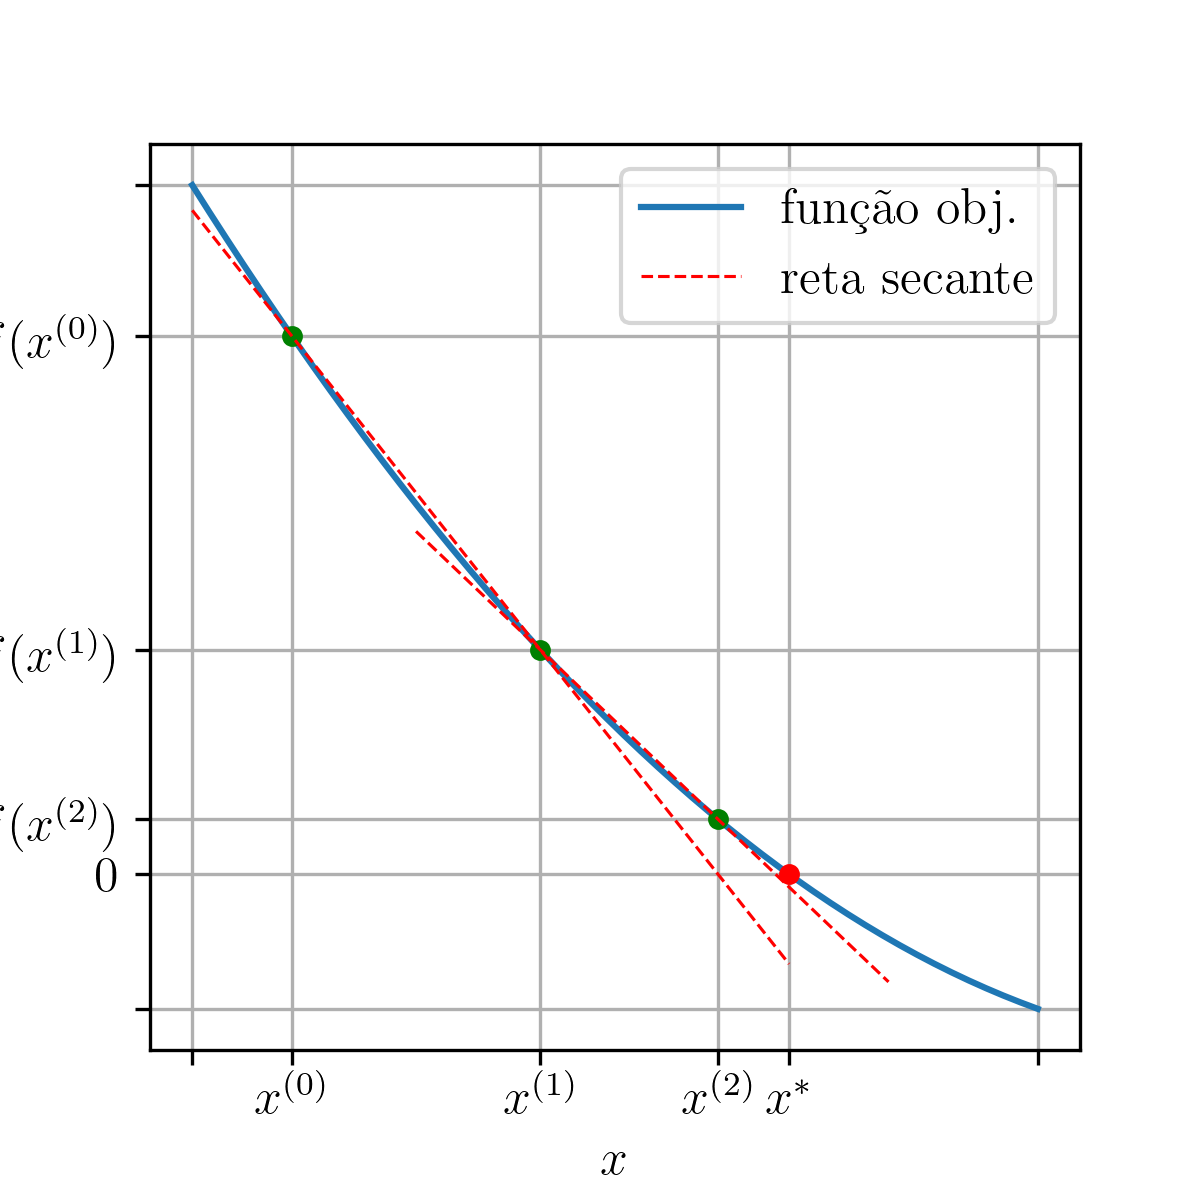
\includegraphics[width=\textwidth]{./cap_eq1d/dados/fig_secante_geointerp/fig}
  \caption{Interpretação geométrica do Método da Secante.}
  \label{cap_eq1d_sec_secante:fig:secante_geointerp}
\end{figure}


\begin{obs}\normalfont{\hl{(Aproximações iniciais.)}}
  A interpretação geométrica do método da secante pode nos ajudar a escolher as aproximações iniciais $x^{(1)}$ e $x^{(2)}$. Como uma boa prática, escolhemo-las próximas do zero (por inspeção gráfica), tomando $x^{(1)}$ como uma aproximação melhor que $x^{(0)}$. 
\end{obs}

\begin{obs}\normalfont{\hl{(Ordem de convergência super-linear.)}}
  A ordem de convergência do Método da Secante é superlinear com
  \begin{equation}\hleq
    |x^{(k+1)}-x^*| \leq C|x^{(k)}-x^*|^{\pmb{\varphi}},
  \end{equation}
  onde $\varphi = (1+\sqrt{5})/2\approx 1,618$ (\href{https://pt.wikipedia.org/wiki/Propor%C3%A7%C3%A3o_%C3%A1urea}{razão áurea}) e $x^*$ é o zero de $f$.
\end{obs}

\begin{obs}\normalfont{\hl{(Zeros de multiplicidade par.)}}
  A ordem de convergência super-linear do método da secante não se mantém para o caso de $x^*$ ser um zero múltiplo. Para contornar este problema, pode-se aplicar o método à derivada $n-1$ de $f$, a fim de se aproximar um zero de multiplicidade $n$.
\end{obs}

\begin{obs}\normalfont{\hl{(Cancelamento catastrófico.)}}
  Conforme convergem as iterações do método da secante, o denominador $f(x^{(k)})-f(x^{(k-1)})$ pode convergir rapidamente para zero, ocasionando uma divisão por zero.
\end{obs}


\subsection*{Exercícios}

\begin{exer}
  Use o Método da Secante para obter uma aproximação do zero de
  \begin{equation}
    f(x)=x^3\sen(x)-\cos(x)
  \end{equation}
  no intervalo $[0,5, 1]$ com precisão de $10^{-5}$.
\end{exer}
\begin{resp}
  $9,1581\times 10^{-1}$
\end{resp}

\begin{exer}
  Use o Método da Secante para computar a(s) solução(ões) das seguintes equações com precisão de 8 dígitos significativos.
  \begin{enumerate}[a)]
  \item $x = 2^{-x}$ para $0\leq x \leq 2$.
  \item $e^{-x^2} = 3x - x^2$ para $-1\leq x\leq 4$.
  \end{enumerate}
\end{exer}
\begin{resp}
  a) $6.4118574\times 10^{-1}$; b) $3.3536470\times 10^{-1}$; $2.9999589$
\end{resp}

\begin{exer}
  Use o Método da Secante para obter uma aproximação do zero de
  \begin{equation}
    \begin{aligned}
      f(x) &= \sen^2\left(x+\frac{\pi}{4}\right) - x^3 \\
           &+ \frac{\pi}{4}x^2 + \frac{5\pi^2}{16}x + \frac{3\pi^3}{64}.
    \end{aligned}
\end{equation}
  no intervalo $[-1, 0]$ com precisão de $10^-5$. Compare a convergência entre as seguintes abordagens:
  \begin{enumerate}[a)]
  \item aplicando a iteração \eqref{cap_eq1d_sec_secante:eq:iter_secante} diretamente à $f$.
  \item aplicando a iteração \eqref{cap_eq1d_sec_secante:eq:iter_secante} diretamente à $f'$.
  \end{enumerate}
  Qual das duas abordagens tem convergência mais rápida? Justifique sua resposta.
\end{exer}
\begin{resp}
  Dica: $f$ tem um zero de multiplicidade par no intervalo $[-1, 0]$.
\end{resp}

\begin{exer}
  Use o Sétodo da Secante para obter uma aproximação do zero de
  \begin{equation}
    \begin{aligned}
      f(x) &= (-x^2+1,154x-0,332929)\cos(x) \\
           &+ x^2 - 1,154x + 0,332929
    \end{aligned}
\end{equation}
no intervalo $[0,55, ~0,65]$ com precisão de $10^-5$.
\end{exer}
\begin{resp}
  $5,7700\times 10^{-1}$
\end{resp}

\begin{exer}
  Use o Método da Secante para encontrar uma aproximação com precisão de $4$ dígitos significativos do zero de 
  \begin{equation}
    \begin{aligned}
      f(x) &= (-x^2+1,154x-0,332929)\cos(x) + x^2 \\
      &- 1,154x + 0,332929
  \end{aligned}
  \end{equation}
  no intervalo $[-1, 0]$.
\end{exer}
\begin{resp}
  $-7,861\times 10^{-1}$
\end{resp}
bootstra
\begin{exer}
  Use o Método da Secante para encontrar o ponto crítico\endnote{Definimos que $x$ é ponto crítico de uma dada $f$, quando $f'(x) = 0$ ou $\nexists f'(x)$.} de
  \begin{equation}
    f(x) = (1-x^2)e^{-x^2}
  \end{equation}
  no intervalo $[0, 2]$. Obtenha o resultado com precisão de $5$ dígitos significativos por arredondamento.
\end{exer}

\ifisbook
\subsubsection{Respostas}
\shipoutAnswer
\fi

%%% SECTION %%%

\section{Raízes de Polinômios}\label{cap_eq1d_sec_raizes}\index{raízes de!polinômios}
\badgeRevisar

Nesta seção, veremos como o método de Newton pode ser aplicado de forma robusta a polinômios com o auxílio do método de Horner\endnote{William George Horner, matemático britânico, 1786 - 1837. Fonte: \href{https://en.wikipedia.org/wiki/William_George_Horner}{Wikipedia}}. A questão central é que dado um polinômio de grau $n$ escrito na forma
\begin{equation}
  p(x) = a_{1}x^n + a_{2}x^{n-1} + \cdots + a_nx + a_{n+1},
\end{equation}
o procedimento de avaliá-lo em um ponto requer $n!n$ multiplicações e $n$ adições. Desta forma, a aplicação do método de Newton para obter as raízes de $p$ torna-se computacionalmente custosa, por requer a avaliação de $p$ e de sua derivada a cada iteração. Agora, o método de Horner nos permite avaliar $p$ em um ponto qualquer usando apenas $n$ multiplicações e $n$ adições, reduzindo enormemente o custo computacional.

\subsection{Método de Horner}\index{método de!Horner}
\badgeRevisar

Sejam dados um número $x_0$ e um polinômio de grau $n$
\begin{equation}\label{eq:Horner_poli}
  p(x) = p_1x^n + p_2x^{n-1} + \cdots + p_{n}x + p_{n+1}s.
\end{equation}
O método de Horner consiste em computar $p(x_0)$ pela iteração
\begin{align}
  q_1 &= p_1,\label{eq:Horner_b1}\\
  q_{k} &= p_k + q_{k-1}x_0,\quad k=2,3,\dotsc,n+1,\label{eq:Horner_b2}
\end{align}
sendo que, então, $p(x_0) = q_{n+1}$ e, além disso,
\begin{equation}\label{eq:Horner_decomp}
  p(x) = (x-x_0)q(x) + q_{n+1},
\end{equation}
com
\begin{equation}
  q(x) = q_1x^{n-1} + q_2x^{n-2} + \cdots + q_{n-1}x + q_{n}.
\end{equation}

De fato, a verificação de \eqref{eq:Horner_decomp} é direta, uma vez que
\begin{align}
  (x-x_0)q(x)+q_{n+1} &= (x-x_0)(q_1x^{n-1} + q_2x^{n-2} + \cdots + q_{n-1}x + q_{n})\nonumber\\ 
                      &+ q_{n+1}\\
                      &= q_1x^n + (q_2-q_1x_0)^{n-1} + \cdots + (q_{n+1}-q_{n}x_0).
\end{align}
E, então, igualando a $p(x)$ na forma \eqref{eq:Horner_poli}, temos as equações \eqref{eq:Horner_b1}-\eqref{eq:Horner_b2}.

\begin{ex}\label{ex:Horner_exec}
  Consideremos o polinômio
  \begin{equation}
    p(x) = x^3 - 3x^2 + 4.
  \end{equation}
  Para computarmos $p(1)$ pelo método de Horner, tomamos $x_0=1$, $q_1=p_1=1$ e
  \begin{align}
    q_2 &= p_2 + q_1x_0 = -3 + 1\cdot 1 = -2\\
    q_3 &= p_3 + q_2x_0 = 0 + (-2)\cdot 1 = -2\\
    q_4 &= p_4 + q_3x_0 = 4 + (-2)\cdot 1 = 2.
  \end{align}
Com isso, temos $p(3) = q_4 = 4$ (verifique!).

% \ifisoctave
% Para este caso, podemos implementar o método de Horner no \verb+GNU Octave+ com o seguinte \href{https://github.com/phkonzen/notas/blob/master/src/MatematicaNumerica/cap_eq1d/dados/ex_Horner_exec/ex_Horner_exec.m}{código}:
% \verbatiminput{./cap_eq1d/dados/ex_Horner_exec/ex_Horner_exec.m}
% \fi
\end{ex}

\begin{obs}\label{obs:Horner_polider}
  Ao computarmos $p(x_0)$ pelo método de Horner, obtemos a decomposição
  \begin{equation}
    p(x) = (x-x_0)q(x) + b_{n+1}.
  \end{equation}
Desta forma, temos
\begin{equation}
  p'(x) = q(x) + (x-x_0)q'(x),
\end{equation}
donde temos que $p'(x_0) = q(x_0)$. Com isso, para computarmos $p'(x_0)$ podemos aplicar o método de Horner a $q(x)$.

% \ifisoctave
% A implementação do método de Horner no \verb+GNU Octave+ para computar $p(x_0)$ e $p'(x_0)$ pode ser feita com o seguinte \href{https://github.com/phkonzen/notas/blob/master/src/MatematicaNumerica/cap_eq1d/dados/obs_Horner_fun/Horner.m}{código}:
% \verbatiminput{./cap_eq1d/dados/obs_Horner_fun/Horner.m}
% \fi
\end{obs}

\subsection{Método de Newton-Horner}
\badgeRevisar

A implementação do método de Newton a polinômios pode ser feita de forma robusta com o auxílio do método de Horner. Dado um polinômio $p$ e uma aproximação inicial $x^{(1)}$ para uma de suas raízes reais, a iteração de Newton consiste em
\begin{equation}
  x^{(k+1)} = x^{(k)} - \frac{p(x^{(k)})}{p'(x^{(k)})},
\end{equation}
na qual podemos utilizar o método de Horner para computar $p(x^{(k)})$ e $p'(x^{(k)})$.

\begin{ex}\label{ex:poli_Newton}
  Consideremos o caso de aplicar o método de Newton para obter uma aproximação da raiz $x=-1$ de
  \begin{equation}
    p(x) = x^3 - 3x^2 + 4,
  \end{equation}
  com aproximação inicial $x^{(1)} = -2$. Na Tabela \ref{tab:ex_poli_Newton} temos os resultados obtidos.

\begin{table}[h!]
  \centering
  \caption{Resultados referentes ao Exemplo \ref{ex:poli_Newton}.}
  \label{tab:ex_poli_Newton}
  \begin{tabular}{r|cc}
    $k$ & $x^{(k)}$ & $|x^{(k)}-x^{(k-1)}|$ \\\hline
    1 & $-2,0000$ & -x- \\
    2 & $-1,3333$ & $6,7\E-1$ \\
    3 & $-1,0556$ & $2,8\E-1$ \\
    4 & $-1,0019$ & $5,4\E-2$ \\
    5 & $-1,0000$ & $1,9\E-3$ \\\hline
  \end{tabular}
\end{table}

\end{ex}

\subsection{Exercícios}

\badgeRevisar

\begin{exer}
  Use o método de Newton-Horner para computar a aproximação da raiz de $p(x) = x^3 - 3x^2 + 4$ no intervalo $[1,3]$. Observe que $p$ tem um zero duplo deste intervalo.
\end{exer}
\begin{resp}
  % \ifisoctave 
  % \href{https://github.com/phkonzen/notas/blob/master/src/MatematicaNumerica/cap_eq1d/dados/exer_NewtonHorner_multpar/exer_NewtonHorner_multpar.m}{Código.} 
  % \fi
  $2$
\end{resp}

\ifisbook
\subsubsection{Respostas}
\shipoutAnswer
\fi

%%% SECTION %%%
\chapter{Sistemas Lineares}\label{cap_sislin}
\badgeRevisar

Neste capítulo, estudamos métodos numéricos para a resolução de sistemas lineares de médio e grande porte. Salvo explicitado ao contrário, assume-se que os sistemas são quadrados e têm solução única.

\section{Matrizes Esparsas}\label{cap_sislin_sec_matesparsa}
\badgeRevisar

\hl{Uma matriz é dita ser \emph{esparsa} quando ela tem apenas poucos elementos não nulos}. A ideia é que os elementos não nulos não precisam ser guardados na memória do computador, gerando um grande benefício na redução da demanda de armazenamento de dados. O desafio está no desenvolvimento de estruturas de dados para a alocação eficiente de tais matrizes, i.e. que sejam suficientemente adequadas para os métodos numéricos conhecidos.

\begin{figure}[H]
  \centering
  \includegraphics[width=0.45\textwidth]{./cap_sislin/dados/matriz_esparsa_estruturada/main}\\
  \includegraphics[width=0.45\textwidth]{./cap_sislin/dados/matriz_esparsa_nao_estruturada/main}
  \caption{Em cima: exemplo de uma matriz esparsa estruturada. Em baixo: exemplo de uma matriz esparsa não-estruturada.}
  \label{fig:ex_matriz_esparsa_estrutura}
\end{figure}

\hl{Matrizes esparsas podem ser classificadas como \textbf{estruturadas} ou \textbf{não-estruturadas}}. Uma matriz estruturada é aquela em que as entradas não-nulas formam um padrão regular. Por exemplo, estão dispostas em poucas diagonais ou formam blocos (submatrizes densas) ao longo de sua diagonal principal. No caso de não haver um padrão regular das entradas não-nulas, a matriz esparsa é dita ser não-estruturada. Consulte a Figura \ref{fig:ex_matriz_esparsa_estrutura} para exemplos.

\hl{A \textbf{esparsidade} de uma matriz é a porcentagem de elementos nulos que ela tem}, i.e. para uma matriz quadrada $n\times n$ tem-se que a esparsidade é
\begin{equation}\hleq
  e := \frac{n_{\text{nulos}}}{n^2}\times 100\%.
\end{equation}
Por exemplo, a matriz identidade de tamanho $n=100$ tem esparsidade
\begin{equation}
  e = \frac{100^2 - 100}{100^2}\times 100\% = 99\% .
\end{equation}

\subsection{Sistemas Tridiagonais}
\badgeRevisar

Um \hlemph{sistema tridiagonal} tem a seguinte forma matricial
\begin{equation}\label{eq:sistridiag}
  \begin{bmatrix}
    a_{1,1} & {\color{violet}a_{1,2}} & & & & 0\\
    {\color{teal}a_{2,1}} & a_{2,2} & {\color{violet}a_{2,3}} & & &\\
    & {\color{teal}a_{3,2}} & a_{3,3} & {\color{violet}a_{3,4}} & &\\
    & & \ddots & \ddots & \ddots &\\
    & & & \ddots & \ddots & {\color{violet}a_{n-1,n}}\\
    0 & & & & {\color{teal}a_{n,n-1}} & a_{n,n}
  \end{bmatrix}
  \begin{bmatrix}
    x_1\\
    x_2\\
    x_3\\
    \vdots\\
    x_{n-1}\\
    x_n
  \end{bmatrix} =
    \begin{bmatrix}
    b_1\\
    b_2\\
    b_3\\
    \vdots\\
    b_{n-1}\\
    b_n
  \end{bmatrix}.
\end{equation}
Ou seja, \hl{é um sistema cuja a matriz dos coeficientes é tridiagonal}.

\hl{Uma \emph{matriz tridiagonal} é uma matriz esparsa estruturada}. Mais especificamente, é um caso particular de uma \hlemph{matriz banda}, em que os elementos não nulos estão dispostos apenas em algumas de suas diagonais. Para armazenarmos tal matriz precisamos alocar apenas os seguintes três vetores
\begin{align}
  & {\color{violet}d_{1} = \left(0,a_{1,2},\dotsc,a_{n-1,n}\right)},\\
  & d_{0} = \left(a_{1,1},a_{2,2},\dotsc,a_{n,n}\right),\\
  & {\color{teal}d_{-1} = \left(a_{2,1},\dotsc,a_{n,n-1},0\right)}.
\end{align}
Ou seja, precisamos armazenar $3n$ pontos flutuantes em vez de $n^2$, como seria o caso se a matriz dos coeficientes fosse densa. Com isso, podemos alocar a matriz do sistema da seguinte forma
\begin{equation}
  \tilde{A} =
  \begin{bmatrix}
    {\color{violet}*} & {\color{violet}a_{1,2}} & {\color{violet}\cdots} & {\color{violet}a_{n-1,n}}\\
    a_{1,1} & a_{2,2} & \cdots & a_{n,n}\\
    {\color{teal}a_{2,1}} & {\color{teal}\dotsc} & {\color{teal}a_{n,n-1}} & {\color{teal}*}
  \end{bmatrix}.
\end{equation}
Ou seja, $\tilde{A} = [\tilde{a}_{i,j}]_{i,j=1}^{3,n}$, sendo
\begin{equation}
  \tilde{a}_{1+i-j,j} = a_{i,j}.
\end{equation}

\begin{ex}
  Seja o seguinte sistema linear
  \begin{gather}
    2x_1 - x_2 = 0\\
    x_{i-1} - 6x_i + 4x_{i+1} = \sen\left(i\frac{\pi}{2(n-1)}\right)\\
    x_{n-1} + x_n = 1
  \end{gather}
  
  O seguinte código {\python} faz a alocação de seu vetor dos termos constantes $b$ e de sua matriz de coeficientes no formato compacto de $\tilde{A}$.

\begin{lstlisting}[caption=diagSis.py, label={py:diagSis}]
import numpy as np
n = 100000

# alocação
# vetor dos termos constantes
b = np.empty(n)
b[0] = 0.
for i in range(1,n-1):
  b[i] = np.sin(i*np.pi/(2*(n-1)))
b[n-1] = 1.
print(b)
print(f"b size: {b.size*b.itemsize/1024} Kbytes")

# matriz compacta
tA = np.zeros((3,n))

# indexação
def ind(i,j):
return 1+i-j,j

tA[ind(0,0)] = 2.
tA[ind(0,1)] = -1.
for i in range(1,n-1):
  tA[ind(i,i-1)] = 1.
  tA[ind(i,i)] = -3.
  tA[ind(i,i+1)] = 4.
tA[ind(n-1,n-2)] = 1.
tA[ind(n-1,n-1)] = 1.
print(tA)
print(f"tA size: {tA.size*tA.itemsize/1024**2:1.1f} Mbytes")
\end{lstlisting}

\end{ex}

\subsubsection{Algoritmo de Thomas (TDMA)}
\badgeRevisar

\hl{O \emph{algoritmo de Thomas}{\thomas} ou \emph{TDMA} (do inglês, \textit{Tridiagonal Matrix Algorithm}) é uma forma otimizada do método de eliminação gaussiana}{\gauss}\hl{ aplicada a sistemas tridiagonais}. Enquanto este requer $O(n^3)$ operações, esse demanda apenas $O(n)$.

Eliminando os termos abaixo da diagonal em \eqref{eq:sistridiag}, obtemos o sistema equivalente
\begin{equation}
  \begin{bmatrix}
    a_{1,1} & a_{1,2} & & & 0 & | & b_1\\
      & \tilde{a}_{2,2} & a_{2,3} & & & | & \tilde{b}_2\\
    &  & \tilde{a}_{3,3} & \ddots & & | & \vdots \\
    & & & \ddots & a_{n-1,n} & | & \tilde{b}_{n-1}\\
    0 & & & & \tilde{a}_{n,n} & | & \tilde{b}_n
  \end{bmatrix}
\end{equation}
Este é obtido pela seguinte iteração
\begin{align}
  & w \leftarrow \frac{a_{i+1,i}}{a_{i,i}}\\
  & a_{i,i} \leftarrow a_{i,i} - w\cdot a_{i-1,i}\\
  & b_i \leftarrow b_i - w\cdot b_{i-1}
\end{align}
onde, o {\textasciitilde} foi esquecido de propósito, indicando a reutilização da matriz $\tilde{A}$ e do vetor $b$. A solução do sistema é, então, obtida de baixo para cima, i.e.
\begin{gather}
  x_n \leftarrow \frac{b_n}{a_{n,n}}\\
  x_i \leftarrow \frac{b_i - a_{i,i+1}x_{i+1}}{a_{i,i}},
\end{gather}
com $i=n-1,n-2,\dotsc,1$.

\begin{lstlisting}[caption=tdma.py, label={py:tdma}]
def tdma(ta, b):
  a = ta.copy()
  x = b.copy()
  # eliminação
  for i in range(1,n):
    w = a[2,i-1]/a[1,i-1]
    a[1,i] -= w * a[0,i]
    x[i] -= w * x[i-1]
  # resolve
  x[n-1] = x[n-1]/a[1,n-1]
  for i in range(n-2,-1,-1):
    x[i] = (x[i] - a[0,i+1]*x[i+1])/a[1,i]
  return x
\end{lstlisting}


\subsection{Matrizes Banda}
\badgeRevisar

\hl{Uma \emph{matriz banda} é aquela em que os elementos não nulos estão dispostos em apenas algumas de suas diagonais}. Consulte a Figura \ref{fig:MatrizBanda}.

\begin{figure}[H]
  \centering
  \includegraphics[width=0.45\textwidth]{./cap_sislin/dados/figMatrizBanda/main}
  \caption{Exemplo de uma matriz banda.}
  \label{fig:MatrizBanda}
\end{figure}

\begin{ex}\label{ex:poisson}
  Consideramos o seguinte problema de Poisson{\poisson}
  \begin{align}
    &- \Delta u = f(x,y),~(x, y)\in (0, \pi)\times (0, \pi),\\
    &u(0, y) = 0,~y\in [0, \pi],\\
    &u(\pi, y) = 0,~y\in [0, \pi],\\
    &u(x, 0) = 0,~x\in [0, \pi],\\
    &u(x, \pi) = 0,~x\in [0, \pi],
  \end{align}
  onde, $\Delta := \left(\frac{\p^2}{\p x^2}, \frac{\p^2}{\p y^2}\right)$ é o operador laplaciano{\laplace}. Para fixarmos as ideias, vamos assumir
  \begin{equation}
    f(x,y) = \sen(x)\sen(y)
  \end{equation}
  
  Vamos empregar o \textbf{método de diferenças finitas} para computar uma aproximação para a sua solução. Começamos assumindo uma malha uniforme de $n^2$ nodos
  \begin{align}
    & x_i = (i-1)h\\
    & y_j = (j-1)h
  \end{align}
  com tamanho de malha $h = \pi/(n-1)$, $i=1,2,\dotsc,n$ e $j=1,2,\dotsc,n$. Empregando a fórmula de diferenças central, encontramos o seguinte problema discreto associado
  \begin{align}
    &u_{i, 1} = u_{1, j} = 0\\
    &~\nonumber\\
    &- \frac{1}{h^2}u_{i-1,j} - \frac{1}{h^2}u_{i,j-1} + \frac{4}{h^2}u_{i,j} \nonumber\\
    &\qquad- \frac{1}{h^2}u_{i+1,j} - \frac{1}{h^2}u_{i,j+1} = f(x_i, y_j)\\
    &~\nonumber\\
    &u_{i,n} = u_{n,j} = 0
  \end{align}

  Este é um sistema linear $n^2 \times n^2$. Tomando em conta as condições de contorno, ele pode ser reduzido a um sistema $(n-2)^2\times (n-2)^2$
  \begin{equation}
    Aw = b
  \end{equation}
  usando a enumeração das incógnitas 
  \begin{equation}
    (i,j) \rightarrow k=i-1 + (j-2)(n-2), 
  \end{equation}
  i.e.
  \begin{equation}
    u_{i,j} = w_{k=i-1 + (j-2)(n-2)}
  \end{equation}
para $i,j=2,\dotsc,n-2$. Consulte a Figura \ref{fig:malha2d} para uma representação da enumeração em relação a malha.

  \begin{figure}[H]
    \centering
    \includegraphics[width=5in]{./cap_sislin/dados/figMalha2D/fig}
    \caption{Representação da enumeração das incógnitas referente ao problema discutido no Exemplo \ref{ex:poisson}.}
    \label{fig:malha2d}
  \end{figure}

  Afim de obtermos uma matriz diagonal dominante, vamos ordenar as equações do sistema discreto como segue
  \begin{itemize}
  \item $j=2$, $i=2$:
    \begin{equation}\label{cap_sislin_sec_matesparsa:eq:ex_poisson_deq0}
      4w_k - w_{k+1} - w_{k+n-2} = h^2f_{i,j}
    \end{equation}
  \item $j=2$, $i=3,\dotsc,n-2$:
    \begin{equation}
      -w_{k-1} + 4w_{k} - w_{k+1} - w_{k+n-2} = h^2f_{i,j}
    \end{equation}
  \item $j=2$, $i=n-1$:
    \begin{equation}
      -w_{k-1} + 4w_k - w_{k+n-2} = h^2f_{i,j}
    \end{equation}
  \item $j=3,\dotsc,n-2$, $i=2$:
    \begin{equation}
      -w_{k-(n-2)} + 4w_k - w_{k+1} - w_{k+n-2} = h^2f_{i,j}
    \end{equation}
  \item $j=3,\dotsc,n-2$, $i=3,\dotsc,n-2$:
    \begin{equation}
      -w_{k-1} - w_{k-(n-2)} + 4w_k - w_{k+1} - w_{k+n-2} = h^2f_{i,j}
    \end{equation}
  \item $j=3,\dotsc,n-2$, $i=n-1$:
    \begin{equation}
      -w_{k-1} - w_{k-(n-2)} + 4w_k - w_{k+n-2} = h^2f_{i,j} 
    \end{equation}
  \item $j=n-1$, $i=2$:
    \begin{equation}
      -w_{k-(n-2)} + 4w_k - w_{k+1} = h^2f_{i,j}
    \end{equation}
  \item $j=n-1$, $i=3,\dotsc,n-2$:
    \begin{equation}
      -w_{k-1} - w_{k-(n-2)} + 4w_k - w_{k+1} = h^2f_{i,j}
    \end{equation}
  \item $j=n-1$, $i=n-1$:
    \begin{equation}
      -w_{k-1} - w_{k-(n-2)} + 4w_k = h^2f_{i,j}\label{cap_sislin_sec_matesparsa:eq:ex_poisson_deq1}
    \end{equation}
  \end{itemize}
  Com isso, temos um sistema com matriz com 5 bandas, consulte a Figura \ref{fig:exPoissonMatriz}.

  \begin{figure}[H]
    \centering
    \includegraphics[width=0.7\textwidth]{./cap_sislin/dados/figExPoissonMatriz/fig}
    \caption{Representação da matriz do sistema discreto construído no Exemplo \ref{ex:poisson}.}
    \label{fig:exPoissonMatriz}
  \end{figure}
\end{ex}


\subsection{Esquemas de Armazenamento}
\badgeRevisar

A ideia é armazenar apenas os elementos não-nulos de uma matriz esparsa, de forma a economizar a demanda de armazenamento computacional. Cuidados devem ser tomados para que a estrutura de armazenamento utilizada seja adequada para a computação das operações matriciais mais comuns.

\subsubsection{Formato COO}
\badgeRevisar

O \hlemph{formato COO} (do inglês, \textit{COOrdinate format}) é o esquema de armazenamento simples de matrizes esparsas. As estrutura de dados consiste em três arranjos:
\begin{enumerate}[1.]
  \item um arranjo contendo as entradas não-nulas da matriz; 
  \item um arranjo contendo seus índices de linha; 
  \item um arranjo contendo seus índices de coluna.
\end{enumerate}
O método {\PYTHONscipyDOTsparseDOTcooArray} permite a alocação de matrizes no formato COO. 

\begin{ex}\label{ex:coo}
  O seguinte código armazena a matriz
  \begin{equation}
    A =
    \begin{bmatrix}
      2. & 0. & 1.  & 0.\\
      0. & 3. & 2.  & -1.\\
      0  & -1 & -2. & 0.\\
      0  & 0  & 0   & 1.
    \end{bmatrix}
  \end{equation}
  no formato COO.

\begin{lstlisting}
import numpy as np
from scipy.sparse import coo_array

data = np.array([2.,1.,3.,2.,-1.,-1.,-2.,1.])
row = np.array([0,0,1,1,1,2,2,3])
col = np.array([0,2,1,2,3,1,2,3])
Acoo = coo_array((data, (row, col)), shape=(4,4))
print("Acoo = \n", Acoo)
print("A = \n", Acoo.toarray())
\end{lstlisting}

\end{ex}

\begin{flushleft}
\hl{Vantagens do formato COO}
\end{flushleft}
\begin{itemize}
  \item Permite a entrada de dados duplicados (simplicidade).
  \item Conversão rápida para os formatos CSR e CSC\endnote{CSR e CSC são formatos de matrizes esparsas mais eficientes para a computação matricial.}.
\end{itemize}

\begin{flushleft}
  \hl{Desavantagens do formato COO}
\end{flushleft}
\begin{itemize}
  \item complexidade em operações aritméticas.
  \item complexidade na extração de submatrizes.
\end{itemize}

\begin{obs}\normalfont{(\hl{Entradas Duplicadas}.)}
  O formato COO permite a entrada duplicada de elementos da matriz. Na conversão para outros formatos (por exemplo, CSR ou CSC), as entradas duplicadas são somadas.
\end{obs}

\subsubsection{Formato CSR}
\badgeRevisar

O \hlemph{formato CSR} (do inglês, \textit{Compressed Sparse Row}) é uma variação do COO que busca diminuir a alocação de dados repetidos. Assim como o COO, o formato conta com três arranjos $d$, $c$, $p$:
\begin{itemize}
\item $d$ é o arranjo contendo os elementos não-nulos da matriz, ordenados por linhas (i.e., da esquerda para direita, de cima para baixo);
\item $c$ é o arranjo contendo o índice das colunas das entradas não-nulas da matriz (como no formato COO);
\item $p$ é um arranjo cujos elementos são a posição no arranjo $c$ em que cada linha da matriz começa a ser representada. O número de elementos de $i$-ésima linha da matriz dado por $p_{j+1}-p_j$.
\end{itemize}
O método {\PYTHONscipyDOTsparseDOTcsrArray} permite a alocação de matrizes no formato CSR. 

\begin{ex}
  No Exemplo \ref{ex:coo}, alocamos a matriz
  \begin{equation}
    A =
    \begin{bmatrix}
      2. & 0. & 1.  & 0. \\
      0. & 3. & 2.  & -1.\\
      0  & -1 & -2. & 0. \\
      0  & 0  & 0   & 1.
    \end{bmatrix}
  \end{equation}
  no formato COO. Aqui, vamos converter a alocação para o formato CSR e, então, verificar seus atributos.

\begin{lstlisting}
from scipy.sparse import csr_array
Acsr = Acoo.tocsr()
print(f'd = {Acsr.data}')
print(f'c = {Acsr.indices}')
print(f'p = {Acsr.indptr}')
\end{lstlisting}

\begin{verbatim}
d = [ 2.  1.  3.  2. -1. -1. -2.  1.]
c = [0 2 1 2 3 1 2 3]
p = [0 2 5 7 8]  
\end{verbatim}
  

  Por exemplo, o elemento \texttt{p[i=2] = 5} aponta para o \texttt{c[k=5] = 1}, o que fornece \texttt{A[i=2,j=1] = d[k] = -1.}. Verifique!
\end{ex}

\begin{flushleft}
  \hl{Vantagens do formato CSR}
\end{flushleft}
\begin{itemize}
  \item operações aritméticas eficientes;
  \item fatiamento por linhas eficiente;
  \item multiplicação matriz vetor eficiente.
\end{itemize}

\begin{flushleft}
  \hl{Desvantagens do formato CSR}
\end{flushleft}
\begin{itemize}
  \item fatiamento por colunas não eficiente;
  \item custo elevado de realocamento com alteração da esparsidade da matriz.
\end{itemize}


\subsubsection{Formato CSC}
\badgeRevisar

O formato CSC (do inglês, \textit{Compressed Sparse Column}) é uma variação análoga do CSR, mas para armazenamento por colunas. O formato conta com três arranjos $d$, $l$, $p$:
\begin{itemize}
\item $d$ é o arranjo contendo os elementos não-nulos da matriz, ordenados por colunas (i.e., de cima para baixo, da esquerda para direita);
\item $l$ é o arranjo contendo o índice das linhas das entradas não-nulas da matriz;
\item $p$ é um arranjo cujos elementos são a posição no arranjo $l$ em que cada coluna da matriz começa a ser representada. O número de elementos de $j$-ésima coluna da matriz dado por $p_{j+1}-p_j$.
\end{itemize}
O método {\PYTHONscipyDOTsparseDOTcscArray} permite a alocação de matrizes no formato CSC. 


\begin{ex}
  No Exemplo \ref{ex:coo}, alocamos a matriz
  \begin{equation}
    A =
    \begin{bmatrix}
      2. & 0. & 1.  & 0. \\
      0. & 3. & 2.  & -1.\\
      0  & -1 & -2. & 0. \\
      0  & 0  & 0   & 1.
    \end{bmatrix}
  \end{equation}
  no formato COO. Aqui, vamos converter a alocação para o formato CSC e, então, verificar seus atributos.

\begin{lstlisting}
  from scipy.sparse import csc_array
  Acsc = Acoo.tocsc()
  l = Acsc.indices
  p = Acsc.indptr
  print(f'd = {Acsc.date}')
  print(f'l = {Acsc.indices}')
  print(f'p = {Acsc.indptr}')
\end{lstlisting}

\begin{verbatim}
  d = [2.  3. -1.  1.  2. -2. -1.  1.]
  l = [0 1 2 0 1 2 1 3]
  p = [0 1 3 6 8]
\end{verbatim}

Assim sendo, o elemento \texttt{p[j=2] = 3} aponta para o \texttt{l[k=3] = 0}, o que informa que \texttt{A[i=0,j=2]=d[k]=1.}. Verifique!
\end{ex}

\begin{flushleft}
  Vantagens do formato CSC
\end{flushleft}
\begin{itemize}
\item fatiamento por colunas eficiente;
\item operações aritméticas eficientes;
\item multiplicação matriz vetor eficiente\footnote{CSR é mais eficiente em muitos casos.}.
\end{itemize}

\begin{flushleft}
  Desvantagens do formato CSC
\end{flushleft}
\begin{itemize}
\item fatiamento por linhas não eficiente;
\item custo elevado de realocamento com alteração da esparsidade da matriz.
\end{itemize}

\begin{obs}
  Além dos formatos COO, CSR e CSC, exitem ainda vários outros que podem empregados e que são mais eficientes em determinadas aplicações. Recomendamos a leitura de \cite[Seção 3.4]{Saad2003} e da documentação do \href{https://docs.scipy.org/doc/scipy/reference/sparse.html}{scipy.sparse}.
\end{obs}

\subsubsection{Exercícios}
\badgeRevisar

\begin{exer}
  Considere o problema de Poisson dado no Exemplo \ref{ex:poisson}.
  \begin{enumerate}[a)]
  \item Armazene a matriz do problema discreto associado usando o formato COO.
  \item Converta a matriz armazenada para o formato CSR\footnote{Use o método \href{https://docs.scipy.org/doc/scipy/reference/generated/scipy.sparse.coo_matrix.tocsr.html}{coo\_matrix.tocsr()}.}. Então, compute a solução do problema discreto com o método \href{https://docs.scipy.org/doc/scipy/reference/generated/scipy.sparse.linalg.spsolve.html}{spsolve}\footnote{\lstinline+scipy.sparse.linalg.spsolve+ é uma implementação do Método LU otimizado para matrizes esparsas.}.
  \item Converta a matriz armazenada para o formato CSC\footnote{Use o método \href{https://docs.scipy.org/doc/scipy/reference/generated/scipy.sparse.coo_matrix.tocsc.html}{coo\_matrix.tocsc()}.}. Então, compute a solução do problema discreto com o método \href{https://docs.scipy.org/doc/scipy/reference/generated/scipy.sparse.linalg.spsolve.html}{spsolve}.
  \item Compare a eficiência da computação entre os itens b) e c) para tamanhos de malha $h = 10^{-1}, 10^{-2}, 10^{-3}, 10^{-4}$.
  \end{enumerate}
\end{exer}

\begin{exer}\label{exer:sislin_tridiag}
  Considere o seguinte sistema linear
  \begin{gather}
    2x_1 - x_2 = 0\\
    x_{i-1} - 6x_i + 4x_{i+1} = \sen\left(i\frac{\pi}{2(n-1)}\right)\\
    x_{n-1} + x_n = 1
  \end{gather}
  \begin{enumerate}[a)]
  \item Compute sua solução usando o Algoritmo de Thomas para $n=3$.
  \item Compare a solução obtida no item anterior com a gerada pela função \href{https://docs.scipy.org/doc/scipy/reference/generated/scipy.linalg.solve.html}{\lstinline+scipy.linalg.solve+}.
  \item Compare a solução com a obtida no item anterior com a gerada pela função \href{https://docs.scipy.org/doc/scipy/reference/generated/scipy.linalg.solve_banded.html}{\lstinline+scipy.linalg.solve_banded+}.
  \item Use o módulo {\python} \href{https://docs.python.org/3/library/datetime.html?highlight=datetime#module-datetime}{datetime} para comprar a demanda de tempo computacional de cada um dos métodos acima. Compute para $n=10,100,1000,10000$.
  \end{enumerate}
\end{exer}

\begin{exer}\label{exer:pvc1d}
  Considere que o problema de valor de contorno (PVC)
  \begin{gather}
    -u'' = \sen \pi x,\quad 0 < x < 1,\\
    u(0) = 0,\\
    u(1) = 0
  \end{gather}
  seja simulado com o Método das Diferenças Finitas\footnote{Consulte mais em \href{https://phkonzen.github.io/notas/MatematicaNumerica/cap_pvc_sec_mdf.html}{Notas de Aula: Matemática Numérica}.}. Vamos assumir uma discretização espacial uniforme com $n$ nodos e tamanho de malha
  \begin{equation}
    h = \frac{1}{n-1}.
  \end{equation}
  Com isso, temos os nodos $x_i = (i-1)h$, $i=1,2,\dotsc,n$. Nos nodos internos, aplicamos a fórmula de diferenças central
  \begin{equation}
    u''(x_i) \approx \frac{u_{i-1} - 2u_i + u_{i+1}}{h^2},
  \end{equation}
  onde, $u_i \approx u(x_i)$. Com isso, a discretização da EDO fornece
  \begin{equation}
    -\frac{1}{h^2}u_{i-1} + \frac{2}{h^2}u_i - \frac{1}{h^2}u_{i+1} = \sen \pi x_i
  \end{equation}
  para $i=2,3,\dotsc,n-1$. Das condições de contorno temos $u_1 = u_n = 0$. Logo, o problema discreto lê-se: encontrar $u = (u_1,u_2,\dotsc,u_n)\in \mathbb{R}^n$ tal que
  \begin{gather}
    u_1 = 0\\
    -\frac{1}{h^2}u_{i-1} + \frac{2}{h^2}u_i - \frac{1}{h^2}u_{i+1} = \sen \pi x_i\\
    u_n = 0
  \end{gather}
  \begin{enumerate}[a)]
  \item Calcule a solução analítica do PVC.
  \item Use a função \href{https://docs.scipy.org/doc/scipy/reference/generated/scipy.linalg.solve_banded.html}{\lstinline+scipy.linalg.solve_banded+} para computar a solução do problema discreto associado para diferentes tamanhos de malha $h = 10^{-1}, 10^{-2}, 10^{-3}, 10^{-4}$. Compute o erro da solução discreta em relação à solução analítica.
  \item Compare a demanda de tempo computacional se a função \href{https://docs.scipy.org/doc/scipy/reference/generated/scipy.linalg.solve.html}{\lstinline+scipy.linalg.solve+} for empregada na computação da solução discreta.
  \end{enumerate}
\end{exer}

\begin{exer}
    Consideremos o problema trabalho no Exemplo \ref{ex:poisson}.
    \begin{enumerate}[a)]
    \item Use a função \href{https://docs.scipy.org/doc/scipy/reference/generated/scipy.linalg.solve.html}{\lstinline+scipy.linalg.solve+} para computar a solução do problema discreto associado para diferentes tamanhos de malha $h = 10^{-1}, 10^{-2}, 10^{-3}, 10^{-4}$. Compute o erro da solução discreta em relação à solução analítica. Compare as aproximações com a solução analítica
      \begin{equation}
        u(x,y) = \frac{1}{2}\sen(x)\sen(y).
      \end{equation}
    \item Compare a demanda de tempo e memória computacional se a função \href{https://docs.scipy.org/doc/scipy/reference/generated/scipy.linalg.solve_banded.html}{\lstinline+scipy.linalg.solve_banded+} for empregada na computação da solução discreta.
    \item Baseado no Algoritmo de Thomas, implemente o Método de Eliminação Gaussiana otimizado para a matriz banda deste problema. Compare com as abordagens dos itens a) e b).
    \end{enumerate}
\end{exer}

%%% Section %%%
\section{Métodos Iterativos}\label{cap_sislin_sec_metiter}
\badgeRevisar

\subsection{GMRES}
\badgeRevisar

O \hlemph{GMRES} (do inglês, \textit{Generalized Minimal Residual Method}\endnote{Desenvolvido por Yousef Saad e H. Schultz, 1986. Fonte: \href{https://en.wikipedia.org/wiki/Generalized_minimal_residual_method}{Wikipedia}.}) é um \hlemph{método de subespaço de Krylov}{\krylov} e é considerado uma das mais eficientes técnicas para a resolução de sistemas lineares gerais e de grande porte (esparsos).

\subsubsection{Método de Subespaço de Krylov}
\badgeRevisar

A ideia básica é resolver o sistema linear
\begin{equation}
  Ax = b
\end{equation}
por um \hlemph{método de projeção}. Mais especificamente, busca-se uma solução aproximada $x_m\in\mathbb{R}^n$ no subespaço afim $x_0 + \mathcal{K}_m$ de dimensão $m$, impondo-se a \hlemph{condição de Petrov}{\petrov}\hlemph{-Galerkin}{\galerkin}
\begin{equation}
  b - Ax_m \perp \mathcal{L}_m,
\end{equation}
onde $\mathcal{L}_m$ também é um subespaço de dimensão $m$. Quando $\mathcal{K}_m$ é um \hlemph{subespaço de Krylov}, i.e.
\begin{equation}
  \mathcal{K}_m(A,r_0) = \spn\{r_0, Ar_0, A^2r_0,\dotsc,A^{m-1}r_0\},
\end{equation}
temos o \hlemph{método de subespaço de Krylov}. Aqui, temos o \emph{resíduo}
\begin{equation}
  r_0 = b - Ax_0,
\end{equation}
sendo $x_0$ uma aproximação inicial para a solução do sistema. Notamos que com isso, temos que a aproximação calculada é tal que
\begin{equation}
  A^{-1}b \approx x_m = x_0 + q_{m-1}(A)r_0,
\end{equation}
onde $q_{m-1}$ é um dado polinômio de grau $m-1$. No caso particular de $x_0 = 0$, temos
\begin{equation}
  A^{-1}b \approx q_{m-1}(A)b.
\end{equation}

Diferentes versões deste método são obtidas pelas escolhas do subespaço $\mathcal{L}_m$ e formas de precondicionamento do sistema.

\subsubsection{GMRES}
\badgeRevisar

O \hlemph{GMRES} é um \emph{método de subespaço de Krylov} assumindo $\mathcal{L}_m = A\mathcal{K}_m$, com
\begin{equation}
  \mathcal{K}_m = \mathcal{K}_m(A,v_1) = \spn\{v_1, Av_1, \dotsc, A^{m-1}v_1\},
\end{equation}
onde $v_1 = r_0/\|r_0\|$ é o vetor unitário do resíduo $r_0 = b - Ax_0$ para uma dada aproximação inicial $x_0$ da solução do sistema $Ax = b$.

Vamos derivar o método observando que qualquer vetor $x$ em $x_0 + \mathcal{K}_m$ pode ser escrito como segue
\begin{equation}
  x = x_0 + V_my
\end{equation}
onde, $V_m = [v_1,\dotsc,v_m]$ é a matriz $n\times m$ cujas colunas formam uma base ortogonal $\{v_1, \dotsc, v_m\}$ de $\mathcal{K}_m$ e $y\in R^m$. Aqui, $V_m$ é computada usando-se o seguinte \hlemph{método de Arnoldi}{\arnoldi}\hlemph{- Gram}{\gram}\hlemph{-Schmidt}{\schmidt} \emph{modificado} \cite[Subseção 6.3]{Saad2003}:
\begin{enumerate}[1.]
\item Dado $v_1$ de norma 1
\item Para $j=1,\dotsc,m$:
  \begin{enumerate}
  \item $w_j \leftarrow Av_j$
  \item Para $i=1,\dotsc,j$:
    \begin{enumerate}
    \item $h_{i,j} \leftarrow (w_j,v_i)$
    \item $w_j \leftarrow w_j - h_{i,j}v_i$
    \end{enumerate}
  \item $h_{j+1,j} \leftarrow \|w_j\|$
  \item Se $h_{j+1,j} \leftarrow 0$, então pare.
  \item $v_{j+1} \leftarrow w_j/h_{j+1,j}$
\end{enumerate}
\end{enumerate}

Seja, então, $\bar{H}_m = [h_{i,j}]_{i,j=1}^{m+1,m}$ a \emph{matriz de Hessenberg}{\hessenberg} cujas entradas não nulas são computadas pelo algoritmo acima (Passos 2(a)i-ii). Pode-se mostrar que \cite[Proposição 6.5]{Saad2003}
\begin{align}
  J(y) &= \|b-Ax\|\\
       &= \|b - A(x_0 + V_my)\|\\
       &= \|\beta e_1 - \bar{H}_my\|
\end{align}
onde, $\beta = \|r_0\|$.

A aproximação GMRES $x_m$ é então computada como
\begin{align}
  x_m &= x_0 + V_my_m,\\
  y_m &= \min_{y} \|\beta e_1 - \bar{H}_my\|
\end{align}
Observamos que este último é um pequeno problema de minimização, sendo que requer a solução de um sistema $(m+1)\times m$ de mínimos quadrados, sendo $m$ normalmente pequeno.


Em resumo, a solução GMRES $x_m$ é computada seguindo os seguintes passos:
\begin{enumerate}[1.]
\item Escolhemos uma aproximação inicial $x_0$ para a solução de $Ax = b$.
\item Computamos o resíduo $r_0 = b - Ax_0$.
\item Computamos o vetor unitário $v_1 = r_0/\|r_0\|$.
\item Usamos o método de Arnoldi-Gram-Schmidt modificado para calculamos uma base ortogonal $V_m$ de $\mathcal{K}_m$ e a matriz de Hessenberg $\bar{H}_m$ associada.
\item Computamos $y_m = \min_{y} \|\beta e_1 - \hat{H}_my\|$.
\item Computamos $x_m = x_0 + V_my$.
\end{enumerate}

\begin{obs}[\hlemph{Convergência}]
  Pode-se mostrar que o GMRES converge em ao menos $n$ passos.
\end{obs}

\begin{obs}[\hlemph{GMRES com a ortogonalização de Householder}]
  No algoritmo acima, o método modificado de Gram-Schmidt é utilizado no processo de Arnoldi. Uma versão numericamente mais eficiente é obtida quando a \hlemph{transformação de Householder}{\householder} é utilizada. Consulte mais em \cite[Subsetion 6.5.2]{Saad2003}.
\end{obs}

\begin{obs}[\hlemph{GMRES com Reinicialização}]
  O \hlemph{restarted GMRES} é uma variação do método para sistemas que requerem uma aproximação GMRES $x_m$ com $m$ grande. Nestes casos, o método original pode demandar um custo muito alto de memória computacional. A ideia consiste em assumir $m$ pequeno e, caso não suficiente, recalcular a aproximação GMRES com $x_0 = x_m$. Este algoritmo pode ser descrito como segue.
  \begin{enumerate}[1.]
  \item Computamos $r_0 = b - Ax_0$, $\beta = \|r_0\|$ e $v_1 = r_0/\beta$
  \item Computamos $V_m$ e $\hat{H}_m$ pelo método de Arnoldi
  \item Computamos
    \begin{gather}
      y_m = \min_y \|\beta e_1 - \hat{H}_my\|\\
      x_m = x_0 + V_my_m
    \end{gather}
  \item Se $\|b-Ax_m\|$ é satisfatória, paramos. Caso contrário, setamos $x_0 := x_m$ e voltamos ao passo 1.
  \end{enumerate}

  \hl{A convergência do restarted GMRES não é garantida para matrizes que não sejam positiva-definidas}.
\end{obs}

\subsubsection{Exercícios}
\badgeRevisar

\begin{exer}\label{exer:pvc1d_gmres}
  Considere o problema discreto do Exercício \ref{exer:pvc1d}.
  \begin{enumerate}[a)]
  \item Compute a solução com a implementação restarted GMRES
    \begin{center}
    \href{https://docs.scipy.org/doc/scipy/reference/generated/scipy.sparse.linalg.gmres.html}{scipy.sparse.linalg.gmres}.
  \end{center}
  \item Por padrão, o intervalo de iterações entre as inicializações é \lstinline+restart=20+. Compare o desempenho para diferentes intervalos de reinicialização.
  \item Compare o desempenho entre as abordagens dos ítens a) e b) frente a implementação do método de eliminação gaussiana disponível em
    \begin{center}
    \href{https://docs.scipy.org/doc/scipy/reference/generated/scipy.sparse.linalg.spsolve.html#scipy.sparse.linalg.spsolve}{scypi.sparse.linalg.spsolve}.
  \end{center}
  \end{enumerate}
\end{exer}

\begin{exer}\label{exer:poisson_gmres}
  Considere o problema discreto trabalhado no Exemplo \ref{ex:poisson}.
  \begin{enumerate}[a)]
  \item Compute a solução com a implementação restarted GMRES
    \begin{center}
\href{https://docs.scipy.org/doc/scipy/reference/generated/scipy.sparse.linalg.gmres.html}{scipy.sparse.linalg.gmres}.
\end{center}
  \item Por padrão, o intervalo de iterações entre as inicializações é \lstinline+restart=20+. Compare o desempenho para diferentes intervalos de reinicialização.
  \item Compare o desempenho entre as abordagens dos ítens a) e b) frente a implementação do método de eliminação gaussiana disponível em
    \begin{center}
\href{https://docs.scipy.org/doc/scipy/reference/generated/scipy.sparse.linalg.spsolve.html#scipy.sparse.linalg.spsolve}{scypi.sparse.linalg.spsolve}.
\end{center}
  \end{enumerate}
\end{exer}

\begin{exer}\label{exer:poissonDNH}
    Considere o seguinte problema de Poisson{\poisson} com condições de contorno não homogêneas.
  \begin{gather}
    - \Delta u = f(x,y),~(x, y)\in D,\\
    u = g, \quad\text{em }\p D
  \end{gather}
  Para fixarmos as ideias, vamos assumir o domínio $D = (0,1)\times (0,1)$, a fonte
  \begin{equation}
    f(x,y) = 2\pi^2 \sen \pi (x+y)
  \end{equation}
  e os valores no contorno
  \begin{equation}
    g = \sen \pi(x+y),\quad (x,y)\in \p D.
  \end{equation}
  Observamos que a solução analítica deste problema é
  \begin{equation}
    u(x,y) = \sen \pi(x+y).
  \end{equation}
  
  Empregue o método de diferenças finitas para computar uma aproximação para a solução. Assumimos uma malha uniforme de $n^2$ nodos
  \begin{gather}
    x_i = (i-1)h\\
    y_j = (j-1)h
  \end{gather}
  com tamanho de malha $h = 1/(n-1)$, $i=1,2,\dotsc,n$ e $j=1,2,\dotsc,n$. Empregando a fórmula de diferenças central encontramos o seguinte problema discreto associado
  \begin{gather}
    u_{i, 1} = g(x_i, 0)\\
    u_{1, j} = g(0, y_j)\\
    ~\nonumber\\
    - \frac{1}{h^2}u_{i-1,j} - \frac{1}{h^2}u_{i,j-1} + \frac{4}{h^2}u_{i,j} \nonumber\\
    - \frac{1}{h^2}u_{i+1,j} - \frac{1}{h^2}u_{i,j+1} = f(x_i, y_j)\\
    ~\nonumber\\
    u_{i,n} = g(x_i, 1)\\
    u_{n,j} = g(1, y_j)
  \end{gather}
  Este pode ser escrito na forma matricial
  \begin{equation}
    Aw = b
  \end{equation}
  onde, $A$ é $(n-2)^2\times (n-2)^2$ e assumindo a enumeração
  \begin{equation}
    u_{i,j} = w_{k=i-1 + (j-2)(n-2)},\quad i,j=2,\dotsc,n-2.
  \end{equation}
  Consulte a Figura \ref{fig:exPoissonMatriz}.

  \begin{enumerate}
  \item Compute a solução do problema discreto associado usando a seguinte implementação {\python} do GMRES
    \begin{center}
      \href{https://docs.scipy.org/doc/scipy/reference/generated/scipy.sparse.linalg.gmres.html}{scipy.sparse.linalg.gmres}
    \end{center}
  \item Compare o desempenho com a aplicação do método LU implemento em
    \begin{center}
      \href{https://docs.scipy.org/doc/scipy/reference/generated/scipy.sparse.linalg.spsolve.html}{scipy.sparse.linalg.spsolve}
    \end{center}
  \end{enumerate}
\end{exer}

\begin{exer}
  Faça sua própria implementação do método GMRES. Valide-a e compare-a com a resolução do exercício anterior (Exercício \ref{exer:poissonDNH}).
\end{exer}


\subsection{Método do Gradiente Conjugado}
\badgeRevisar

O \hlemph{método do gradiente conjugado} é uma das mais eficientes técnicas iterativas para a resolução de sistema linear com matriz esparsa, simétrica e definida positiva. Vamos assumir que o sistema
\begin{equation}
  Ax = b
\end{equation}
onde, a $A$ é \emph{simétrica} e \emph{definida positiva}.

O método pode ser derivado a partir do método de Arnoldi{\arnoldi} \cite[Seção 6.7]{Saad2003} ou como uma variação do método do gradiente. Este é caminho que será adotado aqui.

\subsubsection{Método do Gradiente}
\badgeRevisar

A ideia é reformular o sistema $Ax = b$ como um problema de minimização. Vamos começar definindo o funcional
\begin{equation}\label{eq:funcional_mg}
  J(y) = \frac{1}{2}y^TAy - y^Tb.
\end{equation}
O vetor $y$ que minimiza $J$ é a solução de $Ax = b$. De fato, denotando $x$ a solução de $Ax = b$, temos
\begin{align}
  J(y) &= \frac{1}{2}y^TAy - y^Tb + \frac{1}{2}x^TAx - \frac{1}{2}x^TAx\\
       &= \frac{1}{2}(y-x)^TA(y-x) - \frac{1}{2}x^TAx
\end{align}
O último termo é independente de $y$ e, portanto, $J$ é mínimo quando
\begin{equation}
  \frac{1}{2}(y-x)^TA(y-x)
\end{equation}
é minimizado. Agora, como $A$ é definida positiva\endnote{$x^TAx > 0$ para todo $x\neq 0$.}, o menor valor deste termo ocorre quando $y-x = 0$, i.e. $y=x$.

Observamos, também, que o gradiente de $J$ é
\begin{equation}
  \nabla J = Ay - b
\end{equation}
i.e., é o oposto do resíduo $r = b - Ay$. Com isso, temos que $y = x$ é a única escolha tal que $\nabla J = 0$. Ainda, temos que $\nabla J$ é o vetor que aponta na direção e sentido de maior crescimento de $J$. Isso nos motiva a aplicarmos a seguinte iteração\endnote{Iteração do método do máximo declive.}
\begin{gather}
  x^{(0)} = \text{aprox. inicial}\\
  x^{(k+1)} = x^{(k)} - \alpha_k\nabla J\left(x^{(k)}\right)
\end{gather}
onde, $\alpha_k>0$ é um escalar que regula o tamanho do passo a cada iteração. Lembrando que $-\nabla J = r$, temos que a iteração é equivalente a
\begin{equation}
  x^{(k+1)} = x^{(k)} + \alpha_kr^{(k)}.
\end{equation}
Notamos que $x^{(k+1)}$ é um ponto na reta $\left\{x^{(k)} + \alpha r^{(k)}:~\alpha\in\mathbb{R}\right\}$ que tem a mesma direção de $\nabla J\left(x^{(k)}\right)$ e passa pelo ponto $x^{(k)}$. O procedimento de escolher um $\alpha^{(k)}$ entre todos os possíveis, é conhecido como pesquisa linear (em inglês, \textit{line search}).

A cada iteração, queremos escolher $\alpha_k$ de forma que $J\left(x^{(k+1)}\right) \leq J\left(x^{(k)}\right)$. Isso pode ser garantido fazendo a seguinte escolha\footnote{Chamada de pesquisa linear exata. Qualquer outra escolha para $\alpha$ é conhecida como pesquisa linear não exata.}
\begin{equation}
  J\left(x^{(k+1)}\right) = \min_{\alpha\in\mathbb{R}} J\left(x^{(k)} + \alpha r^{(k)}\right)
\end{equation}
A fim de resolver este problema de minimização, vamos denotar
\begin{gather}
  g(\alpha) = J\left(x^{(k)} + \alpha r^{(k)}\right).
\end{gather}
Então, observamos que
\begin{align}
  g(\alpha) &= \frac{1}{2}\left(x^{(k)} + \alpha r^{(k)}\right)^TA\left(x^{(k)} + \alpha r^{(k)}\right)
              - \left(x^{(k)} + \alpha r^{(k)}\right)^Tb \nonumber\\
            &= \frac{1}{2}{x^{(k)}}^TAx^{(k)} + \frac{\alpha}{2}{x^{(k)}}^TAr^{(k)}  + \frac{\alpha}{2} {r^{(k)}}^TAx^{(k)} \nonumber\\
            & + \frac{\alpha^2}{2}{r^{(k)}}^TAr^{(k)} - {x^{(k)}}^Tb - \alpha {r^{(k)}}^Tb
\end{align}
Agora, usando o fato de $A$ ser simétrica, obtemos
\begin{align}
  g(\alpha) &= J\left(x^{(k)}\right) + \alpha {r^{(k)}}^TAx^{(k)} + \frac{\alpha^2}{2}{r^{(k)}}^TAr^{(k)} - \alpha {r^{(k)}}^Tb\\
            &= J\left(x^{(k)}\right) - \alpha {r^{(k)}}^Tr^{(k)} + \frac{\alpha^2}{2}{r^{(k)}}^TAr^{(k)}
\end{align}
a qual, é uma função quadrática. Seu único mínimo, ocorre quando
\begin{align}
  0 &= g'(\alpha)\\
    &= - {r^{(k)}}^Tr^{(k)} + \alpha {r^{(k)}}^Tb.
\end{align}
Logo, encontramos
\begin{equation}
  \alpha = \frac{{r^{(k)}}^Tr^{(k)}}{{r^{(k)}}^TAr^{(k)}}
\end{equation}

Com isso, temos a iteração do Método do Gradiente
\begin{gather}
  x^{(0)} = \text{aprox. inicial}\\
  x^{(k+1)} = x^{(k)} + \alpha_kr^{(k)},\\
  \alpha_k = \frac{{r^{(k)}}^Tr^{(k)}}{{r^{(k)}}^TAr^{(k)}}
\end{gather}

\begin{obs}[\hlemph{Detalhe de Implementação}]
  Observamos que, a cada iteração, precisamos computar $Ar^{(k)}$ (no cálculo de $\alpha_k$) e $Ax^{(k)}$ (no cálculo do resíduo). Essas multiplicações matriz-vetor são os passos computacionais mais custosos do método. Podemos otimizar isso usando o fato de que
  \begin{equation}
    r^{(k+1)} = r^{(k)} - \alpha_k Ar^{(k)}.
  \end{equation}
\end{obs}


\subsubsection{Exercícios}
\badgeRevisar

\begin{exer}\label{exer:mg}
  Faça sua implementação do método do gradiente.
\end{exer}

\begin{exer}
  Use a implementação feita no Exercício~\ref{exer:mg} nos seguintes itens.
  \begin{enumerate}[a)]
  \item Compute a solução do problema discreto do Exemplo \ref{ex:poisson} pelo Método do Gradiente. Quantas iterações são necessárias para obter um resíduo com norma $\leq 10^{-14}$?
  \item Compute a solução do problema discreto do Exercício \ref{exer:poissonDNH} pelo Método do Gradiente. Quantas iterações são necessárias para obter um resíduo com norma $\leq 10^{-14}$?
  \item Compare a aplicação do método GMRES\endnote{\href{https://docs.scipy.org/doc/scipy/reference/generated/scipy.sparse.linalg.gmres.html}{scipy.sparse.linalg.gmres}} e do método LU\endnote{\href{https://docs.scipy.org/doc/scipy/reference/generated/scipy.sparse.linalg.spsolve.html}{scipy.sparse.linalg.spsolve}} nos itens anteriores.
  \end{enumerate}
\end{exer}

\begin{exer}
  Considere o Exercício~\ref{exer:poissonDNH}.
  \begin{enumerate}[a)]
  \item Use sua implementação do método do gradiente para computar uma solução aproximada, cuja norma do resíduo $\leq 10^{-14}$.
  \item Compare o desempenho com a aplicação da implementação GMRES
    \begin{center}
      \href{https://docs.scipy.org/doc/scipy/reference/generated/scipy.sparse.linalg.gmres.html}{scipy.sparse.linalg.gmres}
    \end{center}
  \end{enumerate}
\end{exer}

\subsubsection{Método do Gradiente Conjugado}
\badgeRevisar

O método do gradiente consiste em uma iteração da forma
\begin{align}
  & x_0 = \text{aprox. inicial},\\
  & x^{(k+1)} = x^{(k)} + \alpha_kp^{(k)},
\end{align}
com $p^{(k)} = r^{(k)}$. Ou seja, a nova aproximação $x^{(k+1)}$ é buscada na direção de $p^{(k)}$. Aqui, a ideia é usar uma melhor direção para buscar a solução.


O \hlemph{método do gradiente conjugado} é um método de gradiente que busca encontrar a solução de $Ax = b$ pela computação do mínimo do seguinte funcional\endnote{Compare com o funcional $J$ dado em \eqref{eq:funcional_mg}.}
\begin{equation}
  J(y) = \frac{1}{2}\left<y,y\right>_A - \left<b,y\right>, 
\end{equation}
onde, $\left<\cdot,\cdot\right>$ denota o produto interno padrão e
\begin{equation}
  \left<x,y\right>_A := x^TAy
\end{equation}
é o \emph{produto interno induzido por $A$}, lembrando que $A$ é positiva definida\endnote{Mostre que $\left<\cdot,\cdot\right>_A$ é de fato um produto interno.}. Associada a este produto interno, temos a norma
\begin{equation}
  \|x\|_A := \sqrt{\left<x,x\right>_A},
\end{equation}
chamada de \emph{norma da energia}. O produto interno associado é também conhecido como \emph{produto interno da energia}. Com isso, definimos que dois vetores $x$ e $y$ são \emph{conjugados}, quando eles são ortogonais com respeito ao produto interno da energia, i.e. quando
\begin{equation}
  \left<x,y\right>_A = 0.
\end{equation}

Aqui, a ideia é desenvolver um método iterativo em que o erro a cada passo seja conjugado a todas as direções de busca anteriores. Consulte o desenvolvimento detalhado do método em \cite[Seção 7.7]{Watkins2002}.

\begin{lstlisting}[caption=Algoritmo do gradiente conjugado, label={code:algGC}]
import numpy as np
import scipy as sp
from scipy.linalg import norm

def mgc(A, b, x, tol=1e-14):
  n, = b.shape
  r = b - A*x
  p = r
  nu = np.dot(r,r)
  for it in np.arange(n):
    q = A*p
    mu = np.dot(p,q)
    alpha = nu/mu
    x = x + alpha*p
    r = r - alpha*q
    nu0 = np.dot(r,r)
    beta = nu0/nu
    p = r + beta*p
    nu = nu0
    if (norm(r) < tol):
      print(it)
      return x
  raise ValueError("Falha de convergencia.")
\end{lstlisting}

\subsubsection{Exercícios}
\badgeRevisar

\begin{exer}\label{exer:mgc}
  Use o Código~\ref{code:algGC} na resolução dos seguintes itens.
  \begin{enumerate}
  \item Compute a solução do problema discreto do Exemplo~\ref{ex:poisson} pelo método do gradiente conjugado. Quantas iterações são necessárias para obter um resíduo com norma $\leq 10^{-14}$?
  \item Compute a solução do problema discreto do Exercício~\ref{exer:poissonDNH} pelo método do gradiente conjugado. Quantas iterações são necessárias para obter um resíduo com norma $\leq 10^{-14}$?
  \item Compare a aplicação do método GMRES\endnote{\href{https://docs.scipy.org/doc/scipy/reference/generated/scipy.sparse.linalg.gmres.html}{scipy.sparse.linalg.gmres}} e da implementação {\scipy} do método do gradiente conjugado\endnote{\href{https://docs.scipy.org/doc/scipy/reference/generated/scipy.sparse.linalg.cg.html}{scipy.sparse.linalg.cg}}
  \end{enumerate}
\end{exer}

\begin{exer}
  Considere o Exercício~\ref{exer:poissonDNH}.
  \begin{enumerate}[a)]
  \item Use sua implementação do método do gradiente conjugado Código~\ref{lst:algGC} para computar uma solução aproximada, cuja norma do resíduo $\leq 10^{-14}$.
  \item Compare o desempenho com a aplicação de sua implementação do método do gradiente (Exercício~\ref{exer:mg}).
  \item Compare o desempenho com a aplicação da implementação GMRES
    \begin{center}
      \href{https://docs.scipy.org/doc/scipy/reference/generated/scipy.sparse.linalg.gmres.html}{scipy.sparse.linalg.gmres}
    \end{center}
  \end{enumerate}
\end{exer}


\subsection{Precondicionamento}
\badgeRevisar

Precondicionamento refere-se a modificar o sistema linear original de forma que a computação de sua solução possa ser feita de forma mais eficiente. No lugar do sistema original
\begin{equation}
  Ax = b
\end{equation}
resolvemos o sistema equivalente
\begin{equation}
  MAx = Mb,
\end{equation}
onde $M = P^{-1}$ e a matriz $P$ é chamada de \emph{precondicionador} do sistema. De forma geral, a escolha do precondicionador é tal que $P \approx A$, mas com inversa fácil de ser computada. Além disso, uma característica esperada é que $MA$ tenha esparsidade parecida com $A$.

\subsubsection{Precondicionamento ILU}
\badgeRevisar

A ideia é tomar $P$ igual a uma fatoração LU incompleta (ILU, do inglês, {\it Incomplete LU}). Incompleta no sentido que entradas de $L$ e de $U$ sejam adequadamente removidas, buscando-se uma boa esparsidade e ao mesmo tempo uma boa aproximação $LU$ para $A$.

\subsubsection{ILU(0)}
\badgeRevisar

O precondicionamento ILU(0) impõe que as matrizes $L$ e $U$ tenham o mesmo padrão de esparsidade da matriz $A$.

\begin{figure}[H]
  \centering
  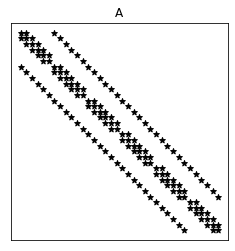
\includegraphics[width=0.45\textwidth]{cap_sislin/dados/figPoissonDnhIlu0/A}~
  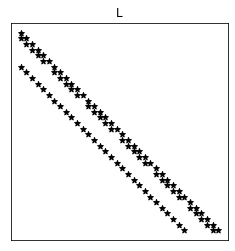
\includegraphics[width=0.45\textwidth]{cap_sislin/dados/figPoissonDnhIlu0/L}\\
  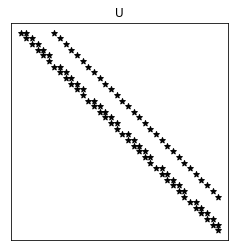
\includegraphics[width=0.45\textwidth]{cap_sislin/dados/figPoissonDnhIlu0/U}~
  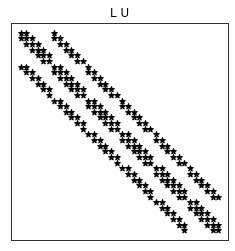
\includegraphics[width=0.45\textwidth]{cap_sislin/dados/figPoissonDnhIlu0/LU}
  \caption{Representação das matrizes ILU(0).}
  \label{fig:poissonDnhIlu0}
\end{figure}

\begin{ex}{ex:possoinDnhIlu0}
  Consideramos o sistema linear $Ax = b$ associado ao problema discreto trabalhado no Exercício \ref{exer:poissonDNH}. Para uma malha $n\times n=8\times 8$, obtemos as matrizes representadas na Figura \ref{fig:poissonDnhIlu0}.

  Observamos que a matriz $LU$ contém duas diagonais com elementos não nulos a mais que a matriz original $A$. Estes elementos são chamados de {\it fill-in}. 
\end{ex}


\lstinputlisting[caption=Algoritmo ILU(0), label={lst:algIlu0}]{./cap_sislin/dados/pyIlu0/main.py}

\subsubsection{Exercícios}
\badgeRevisar

\begin{exer}
  Considere o problema discreto do Exercício \ref{exer:poissonDNH}.
  \begin{enumerate}[a)]
  \item Compute a solução com o método GMRES com precondicionamento ILU(0).
  \item Compare com a resolução com o método GMRES sem precondicionamento.
  \item Compare com a resolução com o método CG sem precondicionamento.
  \item O precondicionamento ILU(0) é eficiente para o método CG?
  \end{enumerate}
\end{exer}

% %Este trabalho está licenciado sob a Licença Atribuição-CompartilhaIgual 4.0 Internacional Creative Commons. Para visualizar uma cópia desta licença, visite http://creativecommons.org/licenses/by-sa/4.0/deed.pt_BR ou mande uma carta para Creative Commons, PO Box 1866, Mountain View, CA 94042, USA.

\chapter{Métodos iterativos para sistemas lineares}\label{cap_sl_iter}
\thispagestyle{fancy}

\section{Métodos de Jacobi e de Gauss-Seidel}\label{cap_sl_iter_sec_jgs}

Nesta seção, discutiremos os métodos de Jacobi\endnote{Carl Gustav Jacob Jacobi, 1804 - 1851, matemático alemão. Fonte: \href{https://en.wikipedia.org/wiki/Carl_Gustav_Jacob_Jacobi}{Wikipedia}.} e de Gauss-Seidel\endnote{Johann Carl Friedrich Gauss, 1777 - 1855, matemático alemão. Philipp Ludwig von Seidel, 1821 - 1896, matemático alemão. Fonte: \href{https://en.wikipedia.org/wiki/Philipp_Ludwig_von_Seidel}{Wikipedia}.} para a aproximação da solução de sistemas lineares.

\subsection{Método de Jacobi}

Dado um sistema $A\pmb{x} = \pmb{b}$ com $n$ equações e $n$ incógnitas, consideramos a seguinte decomposição da matriz $A = L + D + U$:
\begin{align}
  A &=
  \begin{bmatrix}
    a_{11} & a_{12} & a_{13} & \ldots & a_{1n}\\
    a_{21} & a_{22} & a_{23} & \ldots & a_{2n}\\
    a_{31} & a_{32} & a_{33} & \ldots & a_{3n}\\
    \vdots & \vdots & \vdots & \ldots & \vdots\\
    a_{n1} & a_{n2} & a_{n3} & \ldots & a_{nn}\\
  \end{bmatrix}\\
    &= \underbrace{\begin{bmatrix}
    0 & 0 & 0 & \ldots & 0\\
    a_{21} & 0 & 0 & \ldots & 0\\
    a_{31} & a_{32} & 0 & \ldots & 0\\
    \vdots & \vdots & \vdots & \ldots & \vdots\\
    a_{n1} & a_{n2} & a_{n3} & \ldots & 0\\
  \end{bmatrix}}_{L}\\
    &+ \underbrace{\begin{bmatrix}
    a_{11} & 0 & 0 & \ldots & 0\\
    0 & a_{22} & 0 & \ldots & 0\\
    0 & 0 & a_{33} & \ldots & 0\\
    \vdots & \vdots & \vdots & \ldots & \vdots\\
    0 & 0 & 0 & \ldots & a_{nn}\\
  \end{bmatrix}}_{D}\\
  &+ \underbrace{\begin{bmatrix}
    0 & a_{12} & a_{13} & \ldots & a_{1n}\\
    0 & 0 & a_{23} & \ldots & a_{2n}\\
    0 & 0 & a_{33} & \ldots & a_{3n}\\
    \vdots & \vdots & \vdots & \ldots & \vdots\\
    0 & 0 & 0 & \ldots & a_{nn}\\
  \end{bmatrix}}_{U}.
\end{align}
Isto é, a matriz $A$ decomposta como a soma de sua parte triangular inferior $L$, de sua diagonal $D$ e de sua parte triangular superior $U$.

Desta forma, podemos reescrever o sistema $A\pmb{x}=b$ da seguinte forma:
\begin{align}
  A\pmb{x} = \pmb{b} &\Leftrightarrow (L + D + U)\pmb{x} = \pmb{b}\\
         &\Leftrightarrow D\pmb{x} = -(L+U)\pmb{x} + \pmb{b}\\
         &\Leftrightarrow \pmb{x} = -D^{-1}(L+U)\pmb{x} + D^{-1}\pmb{b}.
\end{align}
Ou seja, resolver o sistema $A\pmb{x} = \pmb{b}$ é equivalente a resolver o problema de ponto fixo
\begin{equation}
  \pmb{x} = T_J\pmb{x} + \pmb{c}_J,
\end{equation}
onde $T_J = -D^{-1}(L+U)$ é chamada de \emph{matriz de Jacobi}\index{matriz de!Jacobi} e $\pmb{c}_J = D^{-1}\pmb{b}$ é chamado de \emph{vetor de Jacobi}\index{vetor de!Jacobi}.

\begin{ex}\label{ex:jacobi_intro}
  Consideremos o sistema linear $A\pmb{x} = \pmb{b}$ com
  \begin{equation}
    A =
    \begin{bmatrix}
      -4 & 2 & -1 \\
      -2 & 5 & 2 \\
       1 & -1 & -3
    \end{bmatrix},\quad
    \pmb{b} =
    \begin{bmatrix}
      -11\\ -7\\ 0
    \end{bmatrix}.
  \end{equation}
  Este sistema tem solução $\pmb{x} = (2, -1, 1)$. Neste caso, temos a decomposição $A = L + D + U$ com
  \begin{equation}
    L = \begin{bmatrix} 
      0 & 0 & 0 \\
      -2 & 0 & 0 \\
       1 & -1 & 0
     \end{bmatrix},\quad
    D = \begin{bmatrix}
      -4 & 0 & 0 \\
      0 & 5 & 0 \\
       0 & 0 & -3                  
     \end{bmatrix}
  \end{equation}
  e
  \begin{equation}
    U = \begin{bmatrix}
      0 & 2 & -1 \\
      0 & 0 & 2 \\
       0 & 0 & 0
    \end{bmatrix}.
  \end{equation}
  Ainda, observamos que
  \begin{align}
    T_J\pmb{x} + \pmb{c}_J &= -D^{-1}(L+U)\pmb{x} + D^{-1}\pmb{b}\\
    &= \underbrace{\begin{bmatrix}
        0 & 1/2 & 1/4 \\
        2/5 & 0 & -2/5 \\
        1/3 & -1/3 & 0
      \end{bmatrix}}_{T_J}
      \underbrace{\begin{bmatrix}
        2 \\
        -1 \\
        1             
      \end{bmatrix}}_{\pmb{x}} +
      \underbrace{\begin{bmatrix}
       11/4 \\
       -7/5 \\
       0
      \end{bmatrix}}_{\pmb{c}_J}\\
  &= \underbrace{\begin{bmatrix}
        2 \\
        -1 \\
        1             
      \end{bmatrix}}_{\pmb{x}}.
  \end{align}
% \ifisoctave
% No \verb+GNU Octave+, podemos fazer as computações acima com o seguinte \href{https://github.com/phkonzen/notas/blob/master/src/MatematicaNumerica/cap_sl_iter/dados/ex_jacobi_intro/ex_jacobi_intro.m}{código}:
% \verbatiminput{./cap_sl_iter/dados/ex_jacobi_intro/ex_jacobi_intro.m}
% \fi
\end{ex}

Com o exposto acima, o \emph{método de Jacobi} consiste na seguinte iteração de ponto fixo
\begin{align}
  \pmb{x}^{(1)} &= \text{aprox. inicial},\\
  \pmb{x}^{(k+1)} &= T_J\pmb{x}^{(k)} + \pmb{c}_J,\label{eq:iter_jacobi_mat}
\end{align}
onde $\pmb{x}^{(k)} = (x_1^{(k)}, x_2^{(k)}, \dotsc, x_n^{(k)})$ é a $k$-ésima aproximação (ou iterada) de Jacobi.

A iteração \eqref{eq:iter_jacobi_mat} pode ser equivalentemente escrita na seguinte forma algébrica
\begin{equation}
  x_i^{(k+1)} = \frac{{\displaystyle b_i - \sum_{\overset{j=1}{j\neq i}}^n a_{ij}x_j^{(k)}}}{a_{ii}},~i=1, 2, \dotsc, n,
\end{equation}
a qual não requer a computação da matriz $T_J$ e $\pmb{c}_J$.

\begin{ex}\label{ex:jacobi_exec}
  Consideremos o sistema $A\pmb{x} = \pmb{b}$ com
  \begin{equation}
    A =
    \begin{bmatrix}
      -4 & 2 & -1 \\
      -2 & 5 & 2 \\
       1 & -1 & -3
    \end{bmatrix},\quad
    \pmb{b} =
    \begin{bmatrix}
      -11\\ -7\\ 0
    \end{bmatrix}.
  \end{equation}
  Aplicando o método de Jacobi com aproximação inicial $\pmb{x}^{(1)} = (0, 0, 0)$ obtemos os resultados da Tabela \ref{tab:ex_jacobi_exec}.

  \begin{table}[h!]
    \centering
    \begin{tabular}{l|cc}
      k & $\pmb{x}^{(k)}$ & $\|A\pmb{x}^{(k)}-\pmb{b}\|$\\\hline
      1 & $(0.0,~0.0,~0.0)$ & $1.3\E+1$\\
      2 & $(2.8,~-1.4,~0.0)$ & $7.4\E+0$ \\
      3 & $(2.0,~-0.3,~1.4)$ & $4.6\E+0$ \\
      4 & $(2.3,~-1.1,~0.8)$ & $2.2\E+0$ \\
      5 & $(2.0,~-0.8,~1.1)$ & $1.4\E+0$ \\
      6 & $(2.1,~-1.1,~0.9)$ & $6.9\E-1$ \\
      7 & $(2.0,~-0.9,~1.0)$ & $4.2\E-1$ \\
      8 & $(2.0,~-1.0,~1.0)$ & $2.2\E-1$ \\
      9 & $(2.0,~-1.0,~1.0)$ & $1.3\E-1$ \\
      10 & $(2.0,~-1.0,~1.0)$ & $6.9\E-2$ \\\hline
    \end{tabular}
    \caption{Resultados referentes ao Exemplo \ref{ex:jacobi_exec}.}
    \label{tab:ex_jacobi_exec}
  \end{table}

% \ifisoctave
% No \verb+GNU Octave+, podemos obter os resultados reportados na Tabela \ref{tab:ex_jacobi_exec} com o seguinte \href{https://github.com/phkonzen/notas/blob/master/src/MatematicaNumerica/cap_sl_iter/dados/ex_jacobi_exec/ex_jacobi_exec.m}{código}:
% \verbatiminput{./cap_sl_iter/dados/ex_jacobi_exec/ex_jacobi_exec.m}
% \fi
\end{ex}

\subsection{Método de Gauss-Seidel}

Como acima, começamos considerando um sistema linear $A\pmb{x} = \pmb{b}$ e a decomposição $A = L + D + U$, onde $L$ é a parte triangular inferior de $A$, $D$ é sua parte diagonal e $U$ sua parte triangular superior. Então, observamos que
\begin{align}
  A\pmb{x} = \pmb{b} &\Leftrightarrow (L + D + U)\pmb{x} = \pmb{b}\\
  &\Leftrightarrow (L+D)\pmb{x} = -U\pmb{x} + \pmb{b}\\
  &\Leftrightarrow \pmb{x} = -(L+D)^{-1}U\pmb{x} + (L+D)^{-1}\pmb{b}.
\end{align}
Isto nos leva a iteração de Gauss-Seidel
\begin{align}
  \pmb{x}^{(1)} = \text{aprox. inicial},\\
  \pmb{x}^{(k+1)} = T_G\pmb{x}^{(k)} + \pmb{c}_G,\label{eq:iter_gs_mat}
\end{align}
onde $T_G = -(L+D)^{-1}U$ é a chamada \emph{matriz de Gauss-Seidel}\index{matriz de!Gauss-Seidel} e $\pmb{c}_G = (L+D)^{-1}\pmb{b}$ é o chamado \emph{vetor de Gauss-Seidel}\index{vetor de!Gauss-Seidel}.

Observamos, também, que a iteração \eqref{eq:iter_gs_mat} pode ser reescrita na seguinte forma algébrica
\begin{equation}
  x_i^{(k+1)} = \frac{{\displaystyle b_i - \sum_{j=1}^{i-1} a_{ij}x_j^{(k+1)} - \sum_{j=i+1}^{n} a_{ij}x_j^{(k)}}}{a_{ii}},~i=1, 2, \dotsc, n.
\end{equation}

\begin{ex}\label{ex:gs_exec}
  Consideremos o sistema $A\pmb{x} = \pmb{b}$ com
  \begin{equation}
    A =
    \begin{bmatrix}
      -4 & 2 & -1 \\
      -2 & 5 & 2 \\
       1 & -1 & -3
    \end{bmatrix},\quad
    \pmb{b} =
    \begin{bmatrix}
      -11\\ -7\\ 0
    \end{bmatrix}.
  \end{equation}
  Aplicando o método de Gauss-Seidel com aproximação inicial $\pmb{x}^{(1)} = (0, 0, 0)$ obtemos os resultados da Tabela \ref{tab:ex_gs_exec}.

  \begin{table}[h!]
    \centering
    \begin{tabular}{l|cc}
      k & $\pmb{x}^{(k)}$ & $\|A\pmb{x}^{(k)}-\pmb{b}\|$\\\hline
      1 & $(0.0,~0.0,~0.0)$ & $1.3\E+1$ \\
      2 & $(2.8,~-0.3,~1.0)$ & $2.6\E+0$ \\
      3 & $(2.3,~-0.9,~1.1)$ & $1.2\E+0$ \\
      4 & $(2.0,~-1.0,~1.0)$ & $2.5\E-1$ \\
      5 & $(2.0,~-1.0,~1.0)$ & $4.0\E-2$ \\\hline
    \end{tabular}
    \caption{Resultados referentes ao Exemplo \ref{ex:gs_exec}.}
    \label{tab:ex_gs_exec}
  \end{table}

% \ifisoctave
% No \verb+GNU Octave+, podemos obter os resultados reportados na Tabela \ref{tab:ex_gs_exec} com o seguinte \href{https://github.com/phkonzen/notas/blob/master/src/MatematicaNumerica/cap_sl_iter/dados/ex_gs_exec/ex_gs_exec.m}{código}:
% \verbatiminput{./cap_sl_iter/dados/ex_gs_exec/ex_gs_exec.m}
% \fi
\end{ex}

\subsection{Análise de convergência}

Observamos que ambos os métodos de Jacobi e de Gauss-Seidel consistem de iterações da forma
\begin{equation}
  \pmb{x}^{(k+1)} = T\pmb{x}^{(k)} + \pmb{c},~k=1, 2, \ldots,\label{eq:jgs_iter}
\end{equation}
com $x^{(1)}$ uma aproximação inicial dada, $T$ e $c$ a matriz e o vetor de iteração, respectivamente. O seguinte teorema nos fornece uma condição suficiente e necessária para a convergência de tais métodos.

\begin{teo}
  Para qualquer $\pmb{x}^{(1)}\in\mathbb{R}^n$, temos que a sequência $\{\pmb{x}^{(k+1)}\}_{k=1}^{\infty}$ dada por
  \begin{equation}
    \pmb{x}^{(k+1)} = T\pmb{x}^{(k)} + \pmb{c},
  \end{equation}
  converge para a solução única de $\pmb{x} = T\pmb{x} + \pmb{c}$ se, e somente se, $\rho(T) < 1$\endnote{$\rho(T)$ é o raio espectral da matriz $T$, i.e. o máximo dos módulos dos autovalores de $T$.}.
\end{teo}
\begin{dem}
  Veja \cite[Cap. 7, Sec. 7.3]{Burden2015a}.
\end{dem}

\begin{obs}(\normalfont{Taxa de convergência})
  Para uma iteração da forma \eqref{eq:jgs_iter}, vale
  \begin{equation}
    \|\pmb{x}^{(k)}-\pmb{x}\| \approx \rho(T)^{k-1}\|\pmb{x}^{(1)}-\pmb{x}\|,
  \end{equation}
onde $\pmb{x}$ é a solução de $\pmb{x} = T\pmb{x} + \pmb{c}$.
\end{obs}

\begin{ex}\label{ex:jacobi_exec}
  Consideremos o sistema $A\pmb{x} = \pmb{b}$ com
  \begin{equation}
    A =
    \begin{bmatrix}
      -4 & 2 & -1 \\
      -2 & 5 & 2 \\
       1 & -1 & -3
    \end{bmatrix},\quad
    \pmb{b} =
    \begin{bmatrix}
      -11\\ -7\\ 0
    \end{bmatrix}.
  \end{equation}
  Nos Exemplos \ref{ex:jacobi_exec} e \ref{ex:gs_exec} vimos que ambos os métodos de Jacobi e de Gauss-Seidel eram convergentes, sendo que este convergiu aproximadamente duas vezes mais rápido que esse. Isto é confirmado pelos raios espectrais das respectivas matrizes de iteração
  \begin{equation}
    \rho(T_J) \approx 0.56,\quad\rho(T_G) \approx 0.26.
  \end{equation}

% \ifisoctave
% No \verb+GNU Octave+, podemos obter os raios espectrais das matrizes de iteração de Jacobi e Gauss-Seidel com o seguinte \href{https://github.com/phkonzen/notas/blob/master/src/MatematicaNumerica/cap_sl_iter/dados/ex_jgs_conv/ex_jgs_conv.m}{código}:
% \verbatiminput{./cap_sl_iter/dados/ex_jgs_conv/ex_jgs_conv.m}
% \fi
\end{ex}

\begin{obs}{\normalfont{Matriz estritamente diagonal dominante}}
  Pode-se mostrar que se $A$ é uma matriz estritamente diagonal dominante, i.e. se
  \begin{equation}
    |a_{ii}| > \sum_{\overset{j=1}{j\neq i}}^n |a_{ij}|,~\forall i=1, 2, \ldots, n,
  \end{equation}
então ambos os métodos de Jacobi e de Gauss-Seidel são convergentes.
\end{obs}

\subsection*{Exercícios}

\begin{exer}\label{exer:jacobi_exec}
  Considere o seguinte sistema linear
  \begin{align}
    -4x_1 + x_2 + x_3 - x_4 &= -1\\
    5x_2 -x_3 + 2x_4 &= 3\\
    -x_1 + 4x_3 - 2x_4 &= -2\\
    x_1 -x_2 -5x_4 &= 1
  \end{align}
  Compute a quinta iterada $x^{(5)}$ do método de Jacobi aplicado a este sistema com aproximação inicial $x^{(1)} = (1, 1, -1, -1)$. Também, compute $\|Ax^{(5)} - b\|$.
\end{exer}
\begin{resp}
  %   \ifisoctave 
  %   \href{https://github.com/phkonzen/notas/blob/master/src/MatematicaNumerica/cap_sl_iter/dados/exer_jacobi_exec/exer_jacobi_exec.m}{Código.} 
  % \fi
  $x^{(5)} = (-1.00256,~2.95365,~-1.95347,~0.97913)$; $\|Ax^{(5)}-b\| = 0.42244$
\end{resp}

\begin{exer}\label{exer:gs_exec}
  Considere o seguinte sistema linear
  \begin{align}
    -4x_1 + x_2 + x_3 - x_4 &= -1\\
    5x_2 -x_3 + 2x_4 &= 3\\
    -x_1 + 4x_3 - 2x_4 &= -2\\
    x_1 -x_2 -5x_4 &= 1
  \end{align}
  Compute a quinta iterada $x^{(5)}$ do método de Gauss-Seidel aplicado a este sistema com aproximação inicial $x^{(1)} = (1, 1, -1, -1)$. Também, compute $\|Ax^{(5)} - b\|$.
\end{exer}
\begin{resp}
  %   \ifisoctave 
  %   \href{https://github.com/phkonzen/notas/blob/master/src/MatematicaNumerica/cap_sl_iter/dados/exer_gs_exec/exer_gs_exec.m}{Código.} 
  % \fi
  $x^{(5)} = (-1.00423,~3.00316,~-2.00401,~0.99852)$; $\|Ax^{(5)}-b\| = 0.025883$
\end{resp}

\section{Método do gradiente}\label{cap_sl_iter_sec_metg}

Começamos observando que se $A$ é uma matriz $n\times n$ positiva definida\endnote{$A$ é simétrica e $x^TAx > 0$ para todo $x\neq 0$.}, temos que $\pmb{x}\in\mathbb{R}^n$ é solução de
\begin{equation}\label{eq:metg_sislin}
  A\pmb{x} = \pmb{b}
\end{equation}
se, e somente se, $\pmb{x}$ é solução do seguinte problema de minimização
\begin{equation}\label{eq:metg_minprob}
  \min_{\pmb{x}\in\mathbb{R}^n}f(\pmb{x}) := \frac{1}{2}\pmb{x}^TA\pmb{x}-\pmb{x}^T\pmb{b}.
\end{equation}

O método do gradiente é um algoritmo da forma: dada uma aproximação inicial $\pmb{x}^{(1)}$ da solução de \eqref{eq:metg_minprob} (ou, equivalentemente, de \eqref{eq:metg_sislin}), computamos novas aproximações da forma iterativa
\begin{equation}
  \pmb{x}^{(k+1)} = \pmb{x}^{(k)} + \alpha^{(k)}\pmb{d}^{(k)},\quad k=1, 2, \ldots,
\end{equation}
onde $\alpha^{(k)}$ é o tamanho do passo (um escalar) e $\pmb{d}^{(k)}\in\mathbb{R}^n$ é a direção de busca.

Para escolhermos a direção $\pmb{d}^{(k)}$, tomamos a fórmula de Taylor de $f$ em torno da aproximação $\pmb{x}^{(k)}$
\begin{equation}\label{eq:metg_taylor}
  f(\pmb{x}^{(k+1)}) = f(\pmb{x}^{(k)}) + \alpha^{(k)}\nabla f(\pmb{x}^{(k)})\cdot \pmb{d}^{(k)} + O\left((\alpha^{(k)})^2\right),
\end{equation}
com $\alpha^{(k)}\to 0$, onde $\nabla f$ denota o gradiente de $f$, i.e.
\begin{align}
  \nabla f(\pmb{x}^{(k)}) &= \left(\frac{\p f}{\p x_1}(\pmb{x}^{(k)}), \frac{\p f}{\p x_2}(\pmb{x}^{(k)}), \dotsc, \frac{\p f}{\p x_n}(\pmb{x}^{(k)})\right)\\
  &= A\pmb{x}^{(k)}-\pmb{b}.
\end{align}


De \eqref{eq:metg_taylor}, segue que se
\begin{equation}
  \nabla f(\pmb{x}^{(k)})\cdot \pmb{d}^{(k)} < 0,
\end{equation}
então $f(\pmb{x}^{(k+1)}) < f(\pmb{x}^{(k)})$ se $\alpha^{(k)}$ é suficientemente pequeno. Em particular, podemos escolher
\begin{equation}
  \pmb{d}^{(k)} = -\nabla f(\pmb{x}^{(k)}),
\end{equation}
se $\nabla f(\pmb{x}^{(k)})\neq 0$.

Do exposto acima, temos a \pmb{iteração do método do gradiente}
\begin{align}
  \pmb{x}^{(1)} &= \text{aprox. inicial}\\
  \pmb{x}^{(k+1)} &= \pmb{x}^{(k)} - \alpha^{(k)}\pmb{r}^{(k)},~k=1, 2, \ldots,
\end{align}
onde $\pmb{r}^{(k)}$ é o resíduo da iterada $k$ dado por
\begin{equation}
  \pmb{r}^{(k)} = A\pmb{x^{(k)}}-\pmb{b}.
\end{equation}

\begin{ex}\label{ex:metg_pc}
  Consideremos o sistema $Ax = b$ com
  \begin{equation}
    A =
    \begin{bmatrix}
      2 & -1 & 0 & 0\\
      -1 & 2 & -1 & 0\\
      0 & -1 & 2 & -1 \\
      0 & 0 & -1 & 2
    \end{bmatrix},\quad
    b =
    \begin{bmatrix}
      -3\\
      2\\
      2\\
      -3
    \end{bmatrix}.
  \end{equation}
  Na Tabela \ref{tab:metg_pc} temos os resultados do emprego do método do gradiente com $\pmb{x}^{(1)} = (0, 0, 0, 0)$ e com passo constante $\alpha^{(k)}\equiv 0.5$.

  \begin{table}[h!]
    \centering
    \caption{Resultados referentes ao Exemplo \ref{ex:metg_pc}.}
    \label{tab:metg_pc}
    \begin{tabular}{l|c|c}
      k & $\pmb{x}^{(k)}$ & $\|A\pmb{x}^{(k)}-\pmb{b}\|$\\\hline
      1 & $(0.0,~0.0,~0.0,~0.0)$ & $5.1\E+0$\\
      2 & $(-1.5,~1.0,~1.0,~-1.5)$ & $1.6\E+0$\\
      3 & $(-1.0,~0.8,~0.8,~-1.0)$ & $5.0\E-1$\\
      4 & $(-1.1,~0.9,~0.9,~-1.1)$ & $1.8\E-1$\\
      5 & $(-1.1,~0.9,~0.9,~-1.1)$ & $8.8\E-2$\\
      6 & $(-1.1,~0.9,~0.9,~-1.1)$ & $6.2\E-2$\\
      7 & $(-1.0,~0.9,~0.9,~-1.0)$ & $4.9\E-2$\\
      8 & $(-1.0,~0.9,~0.9,~-1.0)$ & $4.0\E-2$\\
      9 & $(-1.0,~0.9,~0.9,~-1.0)$ & $3.2\E-2$\\
      10 & $(-1.0,~1.0,~1.0,~-1.0)$ & $2.6\E-2$\\
      11 & $(-1.0,~1.0,~1.0,~-1.0)$ & $2.1\E-2$\\\hline
    \end{tabular}
  \end{table}

% \ifisoctave
% No \verb+GNU Octave+, podemos fazer as computações acima com o seguinte \href{https://github.com/phkonzen/notas/blob/master/src/MatematicaNumerica/cap_sl_iter/dados/ex_metg_pc/ex_metg_pc.m}{código}:
% \verbatiminput{./cap_sl_iter/dados/ex_metg_pc/ex_metg_pc.m}
% \fi
\end{ex}

\subsection{Escolha do passo}

Da iteração do método do gradiente, temos que a melhor escolha do passo $\alpha^{(k)}$ é tal que
\begin{equation}
  f(\pmb{x}^{(k)}+\alpha^{(k)}\pmb{r}^{(k)}) = \min_{\alpha > 0} f(\pmb{x}^{(k)}+\alpha\pmb{r}^{(k)}).
\end{equation}
Desta forma,
\begin{align}
  \frac{\dd}{\dd \alpha}f(\pmb{x}^{(k)}+\alpha \pmb{r}^{(k)}) = 0 &\Rightarrow \nabla f(\pmb{x}^{(k+1)})\cdot \pmb{r}^{(k)} = 0,\\
  &\Rightarrow \left(A(\pmb{x}^{(k)}+\alpha^{(k)}\pmb{r}^{(k)})-b\right)\cdot\pmb{r}^{(k)} = 0,\\
  &\Rightarrow (A\pmb{x}^{(k)}-\pmb{b})\cdot\pmb{r}^{(k)}+\alpha^{(k)}\pmb{r}^{(k)}\cdot A\pmb{r}^{(k)} = 0,
\end{align}
donde
\begin{equation}
  \alpha^{(k)} = - \frac{\pmb{r}^{(k)}\cdot\pmb{r}^{(k)}}{\pmb{r}^{(k)}\cdot A\pmb{r}^{(k)}}.
\end{equation}

\begin{ex}\label{ex:metg_alpha}
  Consideremos o sistema $Ax = b$ com
  \begin{equation}
    A =
    \begin{bmatrix}
      2 & -1 & 0 & 0\\
      -1 & 2 & -1 & 0\\
      0 & -1 & 2 & -1 \\
      0 & 0 & -1 & 2
    \end{bmatrix},\quad
    b =
    \begin{bmatrix}
      -3\\
      2\\
      2\\
      -3
    \end{bmatrix}.
  \end{equation}
  Na Tabela \ref{tab:metg_alpha} temos os resultados do emprego do método do gradiente com $\pmb{x}^{(1)} = (0, 0, 0, 0)$ e com passo
  \begin{equation}
    \alpha^{(k)} = - \frac{\pmb{r}^{(k)}\cdot\pmb{r}^{(k)}}{\pmb{r}^{(k)}\cdot A\pmb{r}^{(k)}}.
\end{equation}

  \begin{table}[h!]
    \centering
    \caption{Resultados referentes ao Exemplo \ref{ex:metg_alpha}.}
    \label{tab:metg_alpha}
    \begin{tabular}{l|c|c}
      k & $\pmb{x}^{(k)}$ & $\|A\pmb{x}^{(k)}-\pmb{b}\|$\\\hline
      1 & $(0.0,~0.0,~0.0,~0.0)$ & $5.1\E+0$\\
      2 & $(-1.1,~0.8,~0.8,~-1.1)$ & $1.5\E-1$\\
      3 & $(-1.0,~1.0,~1.0,~-1.0)$ & $3.0\E-2$\\
      4 & $(-1.0,~1.0,~1.0,~-1.0)$ & $8.8\E-4$\\
      5 & $(-1.0,~1.0,~1.0,~-1.0)$ & $1.8\E-4$\\\hline
    \end{tabular}
  \end{table}

% \ifisoctave
% No \verb+GNU Octave+, podemos fazer as computações acima com o seguinte \href{https://github.com/phkonzen/notas/blob/master/src/MatematicaNumerica/cap_sl_iter/dados/ex_metg_alpha/ex_metg_alpha.m}{código}:
% \verbatiminput{./cap_sl_iter/dados/ex_metg_alpha/ex_metg_alpha.m}
% \fi
\end{ex}

\subsection*{Exercícios}

\emconstrucao

\section{Método do gradiente conjugado}\label{cap_sl_iter_sec_metgc}

O método do gradiente conjugado é uma variação do método do gradiente (veja Seção \ref{cap_sl_iter_sec_metg}). Aqui, a solução de um dado sistema $A\pmb{x}=\pmb{b}$, com $A$ uma matriz positiva definida, é computada de forma iterativa por
\begin{align}
  \pmb{x}^{(1)} &= \text{aprox. inicial},\\
  \pmb{d}^{(1)} &= \pmb{r}^{(1)},\\
  &\\
  \pmb{x}^{(k+1)} &= \pmb{x}^{(k)} + \alpha_k\pmb{d}^{(k)},\\
  \alpha^{(k)} &= -\frac{\pmb{r}^{(k)}\cdot \pmb{d}^{(k)}}{\pmb{d}^{(k)}\cdot A\pmb{d}^{(k)}},\\
  \pmb{d}^{(k+1)} &= -\pmb{r}^{(k+1)}+\beta_k\pmb{d}^{(k)},\\
  \beta^{(k)} &= \frac{\pmb{r}^{(k+1)}\cdot A\pmb{d}^{(k)}}{\pmb{d}^{(k)}\cdot A\pmb{d}^{(k)}},
\end{align}
para $k = 1, 2, \ldots$, e $\pmb{r}^{(k)} = A\pmb{x}^{(k)}-\pmb{b}$.

\begin{ex}\label{ex:metgc_exec}
  Consideremos o sistema $Ax = b$ com
  \begin{equation}
    A =
    \begin{bmatrix}
      2 & -1 & 0 & 0\\
      -1 & 2 & -1 & 0\\
      0 & -1 & 2 & -1 \\
      0 & 0 & -1 & 2
    \end{bmatrix},\quad
    b =
    \begin{bmatrix}
      -3\\
      2\\
      2\\
      -3
    \end{bmatrix}.
  \end{equation}
  Na Tabela \ref{tab:metgc_exec} temos os resultados do emprego do método do gradiente conjugado com $\pmb{x}^{(1)} = (0, 0, 0, 0)$.

  \begin{table}[h!]
    \centering
    \caption{Resultados referentes ao Exemplo \ref{ex:metgc_exec}.}
    \label{tab:metgc_exec}
    \begin{tabular}{l|c|c}
      k & $\pmb{x}^{(k)}$ & $\|A\pmb{x}^{(k)}-\pmb{b}\|$\\\hline
      1 & $(0,~0,~0,~0)$ & $5.1\E+0$\\
      2 & $(-1.1,~0.8,~0.8,~-1.1)$ & $1.5\E-1$\\
      3 & $(-1.0,~1.0,~1.0,~-1.0)$ & $0.0\E+0$\\\hline
    \end{tabular}
  \end{table}

% \ifisoctave
% No \verb+GNU Octave+, podemos fazer as computações acima com o seguinte \href{https://github.com/phkonzen/notas/blob/master/src/MatematicaNumerica/cap_sl_iter/dados/ex_metgc_exec/ex_metgc_exec.m}{código}:
% \verbatiminput{./cap_sl_iter/dados/ex_metgc_exec/ex_metgc_exec.m}
% \fi
\end{ex}

\subsection*{Exercícios}

\emconstrucao
%Este trabalho está licenciado sob a Licença Atribuição-CompartilhaIgual 4.0 Internacional Creative Commons. Para visualizar uma cópia desta licença, visite http://creativecommons.org/licenses/by-sa/4.0/deed.pt_BR ou mande uma carta para Creative Commons, PO Box 1866, Mountain View, CA 94042, USA.

\chapter{Métodos para Sistemas Não Lineares}\label{cap_snl}

Neste capítulo, estudamos sobre \hl{métodos para a resolução} de sistemas de equações não lineares. Vamos tratar o caso \hl{de problemas da forma}: encontrar $\pmb{x}\in\mathbb{R}^n$ tal que
\begin{equation}\hleq
  F(\pmb{x}) = \pmb{0},
\end{equation}
onde $F:\mathbb{R}^n\to\mathbb{R}^n$ é uma dada função vetorial.

\section{Método de Newton}\label{cap_snl_sec_newton}

Consideramos o problema de encontrar
\begin{equation}
  \pmb{x} = (x_1, x_2, \dotsc, x_n)\in\mathbb{R}^n
\end{equation}
tal que
\begin{equation}\label{cap_snl_sec_newton:eq:prob0}\hleq
  F(\pmb{x}) = \pmb{0},
\end{equation}
onde $F:\mathbb{R}^n\to\mathbb{R}^n$ é uma dada função vetorial com
\begin{equation}
  F(\pmb{x}) = (f_1(\pmb{x}), f_2(\pmb{x}), \dotsc, f_n(\pmb{x}))\in\mathbb{R}^n.
\end{equation}

Sejam \hl{$\pmb{x}^*$ a solução exata} de \eqref{cap_snl_sec_newton:eq:prob0} e \hl{$\pmb{x}^{(0)}$ uma dada aproximação de $\pmb{x}^*$}. Assim sendo, tomamos a seguinte \hl{expansão de $F$ em polinômio de Taylor}{\taylor}:
\begin{equation}\hleq
  F(\pmb{x}^*) = F(\pmb{x}^{(0)}) + J_F(\pmb{x}^{(0)})(\pmb{x}^*-\pmb{x}^{(0)}) + \pmb{r},
\end{equation}
onde $J_F$ é a \hl{\emph{matriz jacobiana}{\jacobi} de $F$}
\begin{align}
  \hleq{J_F(\pmb{x})} &:= \frac{\p(f_1, f_2, \dotsc, f_n)}{\p(x_1, x_2, \dotsc, x_n)}\\
  &\hleq{:= \begin{bmatrix}
    \frac{\p f_1}{\p x_1} & \frac{\p f_1}{\p x_2} & \ldots & \frac{\p f_1}{\p x_n}\\
    \frac{\p f_2}{\p x_1} & \frac{\p f_2}{\p x_2} & \ldots & \frac{\p f_2}{\p x_n}\\
    \vdots & \vdots & \vdots & \vdots \\
    \frac{\p f_n}{\p x_1} & \frac{\p f_n}{\p x_2} & \ldots & \frac{\p f_n}{\p x_n}\\
  \end{bmatrix}}
\end{align}
e $\|\pmb{r}\|^2\to 0$ quando $\|\pmb{x}^{(0)}-\pmb{x}^*\|\to 0$. 

Daí, como $F(\pmb{x}^*) = \pmb{0}$, segue que
\begin{equation}
  J_F(\pmb{x}^{(0)})(\pmb{x}^*-\pmb{x}^{(0)}) \approx -F(\pmb{x}^{(0)}).
\end{equation}
Então, multiplicando a inversa da jacobiana à esquerda, obtemos
\begin{equation}
  \pmb{x}^*-\pmb{x}^{(0)} \approx - J_F^{-1}(\pmb{x}^{(0)})F(\pmb{x}^{(0)})
\end{equation}
e, também,
\begin{equation}
  \pmb{x}^* \approx \pmb{x}^{(0)} - J_F^{-1}(\pmb{x}^{(0)})F(\pmb{x}^{(0)}).
\end{equation}

O exposto acima nos motiva a \hl{\emph{iteração de Newton}}{\newton}:
\begin{subequations}\hleq
  \begin{align}
    &\pmb{x}^{(0)} = \text{aprox. inicial},\\
    &\pmb{x}^{(k+1)} = \pmb{x}^{(k)} - J_F^{-1}(\pmb{x}^{(k)})F(\pmb{x}^{(k)}),
  \end{align}
\end{subequations}
com $k=0, 1, 2, \ldots$.

\begin{ex}\label{cap_snl_sec_newton:ex:newton_intro}
  Seja o sistema de equações não lineares
  \begin{subequations}
    \begin{align}
      & x_1x_2^2 = x_1^2x_2 - 6,\\
      & x_1^2x_2^3 - 7 = -x_1.
    \end{align}
  \end{subequations}
  Para usarmos o método de Newton, reescrevemos o sistema na seguinte forma
  \begin{subequations}
    \begin{align}
      x_1x_2^2 - x_1^2x_2 + 6 &= 0,\\
      x_1 + x_1^2x_2^3 - 7 &= 0.
    \end{align}
\end{subequations}
  Com isso, identificamos a função objetivo
  \begin{align}
    F(\pmb{x}) &=
    \begin{bmatrix}
      f_1(\pmb{x})\\
      f_2(\pmb{x})
    \end{bmatrix}\\
    &=
    \begin{bmatrix}
      x_1x_2^2 - x_1^2x_2 + 6\\
      x_1 + x_1^2x_2^3 - 7
    \end{bmatrix}
  \end{align}
  e calculamos sua matriz jacobiana
  \begin{align}
    J_F(\pmb{x}) &= \frac{\p(f_1, f_2)}{\p(x_1, x_2)} \\
                 &=
                   \begin{bmatrix}
                     \frac{\p f_1}{\p x_1} & \frac{\p f_1}{\p x_2}\\
                     \frac{\p f_2}{\p x_1} & \frac{\p f_2}{\p x_2}\\
                   \end{bmatrix}\\
                 &=
                   \begin{bmatrix}
                     x_2^2 - 2x_1x_2 & 2x_1x_2-x_1^2\\
                     1+2x_1x_2^3 & 3x_1^2x_2^2
                   \end{bmatrix}
  \end{align}
  Definidas $F$ e $J_F$ e tomando a aproximação inicial
  \begin{equation}
    \pmb{x}^{(0)} = (-1.5, 1.5)
  \end{equation}
  computamos as iterações de Newton e obtemos os resultados apresentados na Tabela \ref{cap_snl_sec_newton:tab:newton_intro}.

  \begin{table}[H]
    \centering
    \caption{Resultados referentes ao Exemplo \ref{cap_snl_sec_newton:ex:newton_intro}.}
    \begin{tabular}{lcc}\toprule
      k & $\pmb{x}^{(k)}$ & $\|F(\pmb{x}^{(k)})\|$\\\midrule
      0 & $(-1.50, 1.50)$ & $1.2\E+0$\\
      1 & $(-1.07, 1.82)$ & $1.2\E+0$\\
      2 & $(-9.95\E-1, 2.00)$ & $7.6\E-2$\\
      3 & $(-1.00, 2.00)$ & $1.2\E-4$ \\
      4 & $(-1.00, 2.00)$ & $2.1\E-9$ \\\bottomrule
    \end{tabular}
    \label{cap_snl_sec_newton:tab:newton_intro}
  \end{table}

\begin{lstlisting}
import numpy as np
import numpy.linalg as npla

def newton(F, J, x0, 
           maxiter=100, tol=1.49e-8):
  print(f'\n{0}: x = {x0}, ' + \
        f'norm = {npla.norm(F(x0)):.1e}')
  info = -1
  for k in range(maxiter):
    x = x0 - npla.inv(J(x0))@F(x0)
    print(f'{k+1}: x = {x}, ' + \
          f'norm = {npla.norm(F(x)):.1e}')
    if (npla.norm(x - x0) < tol):
      info = 0
      break
    x0 = x.copy()
  return x, info

def F(x):
  n = x.size
  y = np.empty(n)
  y[0] = x[0]*x[1]**2 - x[0]**2*x[1] + 6
  y[1] = x[0] + x[0]**2*x[1]**3 - 7
  return y

def J(x):
  n = x.size
  y = np.empty((n,n))
  y[0,0] = x[1]**2 - 2*x[0]*x[1]
  y[0,1] = 2*x[0]*x[1] - x[0]**2
  y[1,0] = 1 + 2*x[0]*x[1]**3
  y[1,1] = 3*x[0]**2*x[1]**2
  return y

x0 = np.array([-1.5, 1.5])
x, info = newton(F, J, x0)
\end{lstlisting}

\end{ex}

\subsection{Análise Numérica}

Para uma função $F$ suficientemente suave e com uma escolha apropriada da aproximação inicial $\pmb{x}^{(0)}$, temos que as \hl{iterações de Newton}
\begin{equation}
  \pmb{x}^{(k+1)} = \pmb{x}^{(k)} - J_F^{-1}(\pmb{x}^{(k)})F(\pmb{x}^{(k)}),
\end{equation}
com $k=0, 1, 2, \ldots$, \hl{são quadraticamente convergentes}\endnote{Para informações mais precisas sobre a convergência do Método de Newton, consulte \cite[Seção 5.3]{Stoer1993a}.}, i.e.
\begin{equation}\hleq
  \|\pmb{x}^{(k+1)} - \pmb{x}^*\| \leq C\|\pmb{x}^{(k)}-\pmb{x}^*\|^2,
\end{equation}
onde $\pmb{x}^*$ é a solução exata, i.e. $F(\pmb{x}^*) = \pmb{0}$.

\begin{ex}\label{cap_snl_sec_newton:ex:newton_conv}
  Consideremos o seguinte sistema de equações não lineares
  \begin{align}
    x_1x_2^2 - x_1^2x_2 + 6 &= 0,\\
    x_1 + x_1^2x_2^3 - 7 &= 0.
  \end{align}
  A Figura \ref{cap_snl_sec_newton:fig:ex_newton_conv} é um esboço do gráfico da $\|F(\cdot)\|$. Este problema foi confeccionado de forma que $\pmb{x}^* = (-1, 2)$. Então, tomando $\pmb{x}^{(0)} = (1.5, 1.5)$ como aproximação inicial, computamos as iterações de Newton para este problema, donde obtemos os resultados reportados na Tabela \ref{cap_snl_sec_newton:tab:ex_newton_conv}. 

  \begin{figure}[h!]
    \centering
    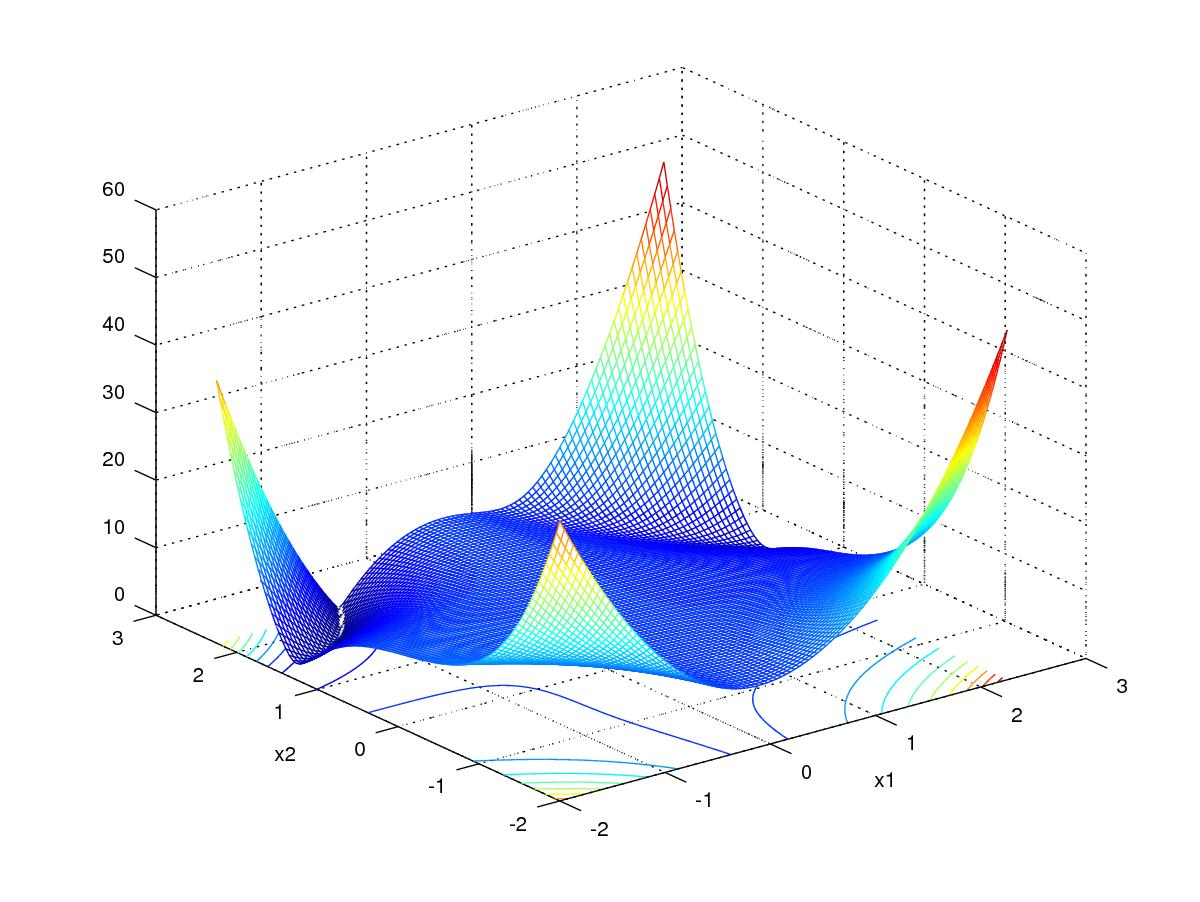
\includegraphics[width=0.7\textwidth]{./cap_snl/dados/ex_newton_conv/ex_newton_conv}
    \caption{Esboço do gráfico de $\|F(\cdot)\|$ referente ao Exemplo \ref{cap_snl_sec_newton:ex:newton_conv}.}
    \label{cap_snl_sec_newton:fig:ex_newton_conv}
  \end{figure}

  \begin{table}[H]
    \centering
    \begin{tabular}{lcc}
      k & $\pmb{x}^{(k)}$ & $\|\pmb{x}^{(k)} - \pmb{x}^*\|$\\\hline
      0 & $(-1.50, 1.50)$ & $7.1\E-01$\\
      1 & $(-1.07, 1.82)$ & $2.0\E-01$\\
      2 & $(-9.95\E-1, 2.00)$ & $5.1\E-03$\\
      3 & $(-1.00, 2.00)$ & $2.6\E-05$ \\
      4 & $(-1.00, 2.00)$ & $2.0\E-10$ \\
      5 & $(-1.00, 2.00)$ & $3.1\E-16$ \\\hline
    \end{tabular}
    \caption{Resultados referentes ao Exemplo \ref{cap_snl_sec_newton:ex:newton_conv}.}
    \label{cap_snl_sec_newton:tab:ex_newton_conv}
  \end{table}
\end{ex}

\subsection{Exercícios}

\begin{exer}
  Use o Método de Newton para computar uma solução aproximada para o sistema de equações
  \begin{subequations}
    \begin{align}
      & \frac{x_1^2}{3} + x_2^2 = 1\\
      & x_1^2 + \frac{x_2^2}{4} = 1
    \end{align}
  \end{subequations}
\end{exer}
\begin{resp}
  Soluções exatas: $\pmb{x} = \pm\left(\sqrt{\frac{9}{11}}, \sqrt{\frac{8}{11}}\right)$.
\end{resp}

\begin{exer}
  Use o Método de Newton, com aproximação inicial $\pmb{x}^{(0)} = (1.5, 0.5)$ para computar uma solução aproximada para o sistema de equações
  \begin{subequations}
    \begin{align}
      & x_1^2 = \cos(x_1x_2) + 1\\
      & \sen(x_2) = 2\cos(x_1)
    \end{align}
  \end{subequations}
\end{exer}
\begin{resp}
  $\pmb{x} = (1.3468109, 0.4603195)$
\end{resp}

\begin{exer}
  Use o Método de Newton, com aproximação inicial $\pmb{x}^{(0)} = (1, -1)$ para computar uma solução aproximada para o sistema de equações
  \begin{subequations}
    \begin{align}
      & 3x_1 = \cos(x_1x_2) + \frac{1}{2}\\
      & 4x_1^2 + 2x_2x_1 = 0
    \end{align}
  \end{subequations}  
\end{exer}
\begin{resp}
  $\pmb{x} = (4.668417\E-1, -9.368334\E-1)$
\end{resp}

\begin{exer}
  Use o método de Newton para obter uma aproximação de uma solução de
  \begin{align}
    x_2\sen(x_3)+x_1-2&=0,\\
    x_1x_2-\sen(x_2)+0.2&=0,\\
    x_3^2+\cos(x_1x_2)-4.5&=0.
  \end{align}
Para tanto, use $\pmb{x}^{(1)} = (1, -1, -1)$.
\end{exer}
\begin{resp}
  $\pmb{x} = (1.7519\E+0, -2.6202\E-1, -1.8983\E+0)$
\end{resp}

\begin{exer}
  Considere o problema de encontrar os pontos de interseção no plano $x-y$ da elipse
  \begin{equation}
    \frac{x^2}{4} + \frac{y^2}{9} = 1
  \end{equation}
  com a curva
  \begin{equation}
    x = y^2\sqrt{x}.
  \end{equation}
  Escreva o problema na forma $F(\pmb{x}) = \pmb{0}$ e use o Método de Newton para encontrar o ponto de interseção próximo de $(x, y) = (1.5, 1.5)$.
\end{exer}
\begin{resp}
  $x = 1.842996\E+0$, $y = 1.165148\E+0$
\end{resp}

\ifisbook
\subsubsection{Respostas}
\shipoutAnswer
\fi

%%% SECTION %%%

\section{Métodos \textit{Quasi}-Newton}\label{cap_snl_sec_quasi_newton}
\badgeRevisar

\subsection{Método do Acorde}
\badgeRevisar

O método do acorde consiste na seguinte iteração
\begin{align}
  \pmb{x}^{(1)} &= \text{aprox. inicial},\\
  \pmb{x}^{(k+1)} &= \pmb{x}^{(k)} - J_F^{-1}(\pmb{x}^{(1)})F(\pmb{x}^{(k)}).
\end{align}
Ou seja, é a iteração de Newton com jacobina constante.

\begin{ex}\label{ex:acorde_exec}
  Consideremos o seguinte sistema de equações não lineares
  \begin{align}
    x_1x_2^2 - x_1^2x_2 + 6 &= 0,\\
    x_1 + x_1^2x_2^3 - 7 &= 0.
  \end{align}
  Definidas $F$ e $J_F$ e tomando $\pmb{x}^{(1)} = (1.5, 1.5)$ como aproximação inicial, computamos as iterações do método do acorde de forma a obtermos os resultados apresentados na Tabela \ref{tab:ex_acorde_exec}.

  \begin{table}[h!]
    \centering
    \begin{tabular}{lcc}
      k & $\pmb{x}^{(k)}$ & $\|\pmb{x}^{(k)} - \pmb{x}^*\|$\\\hline
      1 & $(-1.50, 1.50)$ & -x- \\
      2 & $(-1.07, 1.82)$ & $5.3\E-1$ \\
      3 & $(-1.02, 1.93)$ & $1.2\E-1$ \\
      4 & $(-1.00, 1.98)$ & $5.2\E-2$ \\
      5 & $(-9.98\E-1, 2.00)$ & $1.8\E-2$ \\
      6 & $(-9.98\E-1, 2.00)$ & $4.7\E-3$ \\
      7 & $(-9.99\E-1, 2.00)$ & $9.0\E-4$ \\
      8 & $(-1.00, 2.00)$ & $7.4\E-4$ \\
      9 & $(-1.00, 2.00)$ & $4.3\E-4$ \\\hline
    \end{tabular}
    \caption{Resultados referentes ao Exemplo \ref{ex:acorde_exec}.}
    \label{tab:ex_acorde_exec}
  \end{table}

% \ifisoctave
% No \verb+GNU Octave+, podemos fazer as computações acima com o seguinte \href{https://github.com/phkonzen/notas/blob/master/src/MatematicaNumerica/cap_snl/dados/ex_acorde_exec/ex_acorde_exec.m}{código}:
% \verbatiminput{./cap_snl/dados/ex_acorde_exec/ex_acorde_exec.m}
% \fi
\end{ex}

\subsection{Jacobiana Aproximada}
\badgeRevisar

A jacobiana $J_F(\pmb{x})$ de uma dada função $F(\pmb{x}) = (f_1(\pmb{x}), f_2(\pmb{x}), \dotsc, f_n(\pmb{x}))$ é a matriz cujo elemento da $i$-ésima linha e $j$-ésima coluna é
\begin{equation}
  \frac{\p f_i}{\p x_j} = \lim_{h\to 0} \frac{f_i(\pmb{x}+\pmb{e}_jh) - f_i(\pmb{x})}{h},
\end{equation}
onde $\pmb{e}_j$ é o $j$-ésimo vetor da base canônica de $\mathbb{R}^n$, i.e. $\pmb{e}_j = (0, \dotsc, 0, 1, 0, \dotsc, 0)$ com $1$ na $j$-ésima posição.

Com isso, podemos computar uma jacobiana aproximada tomando
\begin{equation}
  \frac{\p f_i}{\p x_j} \approx \frac{f_i(\pmb{x}+\pmb{e}_jh) - f_i(\pmb{x})}{h},
\end{equation}
com $h$ suficientemente pequeno.

\begin{ex}\label{ex:jacaprox_exec}
  Consideremos o seguinte sistema de equações não lineares
  \begin{align}
    x_1x_2^2 - x_1^2x_2 + 6 &= 0,\\
    x_1 + x_1^2x_2^3 - 7 &= 0.
  \end{align}
  Definida $F$, sua jacobina aproximada $\tilde{J}_F$ com $h=10^{-7}$ e tomando $\pmb{x}^{(1)} = (1.5, 1.5)$ como aproximação inicial, computamos as iterações do {\it quasi}-método de forma a obtermos os resultados apresentados na Tabela \ref{tab:ex_jacaprox_exec}.

  \begin{table}[h!]
    \centering
    \begin{tabular}{lcc}
      k & $\pmb{x}^{(k)}$ & $\|\pmb{x}^{(k)} - \pmb{x}^*\|$\\\hline
      1 & $(-1.50, 1.50)$ & -x- \\
      2 & $(-1.07, 1.82)$ & $5.3\E-1$\\
      3 & $(-9.95\E-1, 2.00)$ & $2.0\E-1$\\
      4 & $(-1.00, 2.00)$ & $5.1\E-3$\\
      5 & $(-1.00, 2.00)$ & $2.6\E-5$\\\hline
    \end{tabular}
    \caption{Resultados referentes ao Exemplo \ref{ex:jacaprox_exec}.}
    \label{tab:ex_jacaprox_exec}
  \end{table}

% \ifisoctave
% No \verb+GNU Octave+, podemos fazer as computações acima com o seguinte \href{https://github.com/phkonzen/notas/blob/master/src/MatematicaNumerica/cap_snl/dados/ex_jacaprox_exec/ex_jacaprox_exec.m}{código}:
% \verbatiminput{./cap_snl/dados/ex_jacaprox_exec/ex_jacaprox_exec.m}
% \fi
\end{ex}

\subsection{Exercícios}

\badgeConstrucao

\ifisbook
\subsubsection{Respostas}
\shipoutAnswer
\fi

%%% SECTION %%%
\chapter{Interpolação}\label{cap_interp}

Neste capítulo, estudamos a \hl{resolução de problemas de interpolação} da forma: dados uma família de $n$ funções reais
\begin{equation}\hleq
  \mathcal{F} = \{f_1(x), f_2(x), \dotsc, f_n(x)\}
\end{equation}
e um conjunto de $n$ pontos $\{(x_i, y_i)\}_{i=1}^n$, com $x_i\neq x_j$ se $i\neq j$, encontrar a \emph{função interpoladora}
\begin{equation}\hleq
  \begin{aligned}
    f(x) = c_1f_1(x) + c_2f_2(x) + \cdots + c_nf_n(x),
  \end{aligned}
\end{equation}
tal que
\begin{equation}\hleq
  y_i = f(x_i),\quad i=1, 2, \ldots, n.
\end{equation}

\section{Interpolação Polinomial}\label{cap_interp_sec_interpoli}

\hl{Dado um conjunto de $n$ pontos $\{(x_i, y_i)\}_{i=1}^n$, o problema de interpolação consiste em encontrar o polinômio}\endnote{Chamado de \emph{polinômio interpolador}.} \hl{de grau $n-1$}
\begin{equation}\label{cap_interp_sec_interpoli:eq:interpoli_poli}\hleq
  \begin{aligned}
    p(x) &= p_1x^{n-1} + p_2x^{n-2} \\
         &+ \cdots + p_{n-1}x + p_n
  \end{aligned}
\end{equation}
tal que
\begin{equation}\label{cap_interp_sec_interpoli:eq:interpoli_conds}\hleq
  y_i = p(x_i),
\end{equation}
para todo $i=1, 2, \dotsc, n$.

Das condições \eqref{cap_interp_sec_interpoli:eq:interpoli_poli}, temos
\begin{equation}\label{cap_interp_sec_interpoli:eq:interpoli_sis}
  \begin{aligned}
    p_1x_1^{n-1} + p_2x_1^{n-2} + \cdots + p_n &= y_1 \\
    p_1x_2^{n-1} + p_2x_2^{n-2} + \cdots + p_n &= y_2 \\
    &\vdots \\
    p_1x_n^{n-1} + p_2x_n^{n-2} + \cdots + p_n &= y_n.
  \end{aligned}
\end{equation}
Isto é, \hl{os coeficientes do \emph{polinômio interpolador} {\eqref{cap_interp_sec_interpoli:eq:interpoli_poli}} satisfazem o sistema linear}
\begin{equation}\hleq
  A\pmb{p} = \pmb{y},
\end{equation}
onde $A$ é a \emph{matriz de Vandermonde}{\vandermonde}
\begin{equation}\hleq
  A =
  \begin{bmatrix}
    x_1^{n-1} & x_1^{n-2} & \ldots & x_1 & 1 \\
    x_2^{n-1} & x_2^{n-2} & \ldots & x_2 & 1 \\
    \vdots  & \vdots  & \vdots  & \vdots & \vdots \\
    x_n^{n-1} & x_n^{n-2} & \ldots & x_n & 1
  \end{bmatrix},
\end{equation}
$\pmb{p} = (p_1, p_2, \ldots, p_n)$ é o \emph{vetor das incógnitas} e $\pmb{y} = (y_1, y_2, \ldots, y_n)$ é o \emph{vetor dos termos constantes}.

\begin{ex}\label{cap_interp_sec_interpoli:ex:interpoli_intro}
  Consideramos o problema de encontrar o polinômio interpolador do conjunto de pontos $\{(-1,~-1), (0, 1), (1, 1/2)\}$. Como temos 3 pontos, o polinômio tem grau 2 e pode ser escrito na forma
  \begin{equation}
    p(x) = p_1x^2 + p_2x + p_3.
  \end{equation}
  Seguindo a abordagem acima, temos $\pmb{p}=(p_1, p_2, p_3)$, $\pmb{x} = (-1, 0, 1)$, $\pmb{y}=(-1, 1, 1/2)$ e
  \begin{equation}
    A =
    \begin{bmatrix}
      x_1^2 & x_1 & 1\\
      x_2^2 & x_2 & 1\\
      x_3^2 & x_3 & 1
    \end{bmatrix}.
  \end{equation}
  Então, resolvendo $A\pmb{p} = \pmb{y}$, obtemos o polinômio interpolador
  \begin{equation}
    p(x) = -1.25x^2 + 0.75x + 1.
  \end{equation}
A Figura \ref{cap_interp_sec_interpoli:fig:interpoli_intro} mostra os esboços do polinômio interpolador $p(x)$ e  dos pontos dados.

\begin{figure}[H]
  \centering
  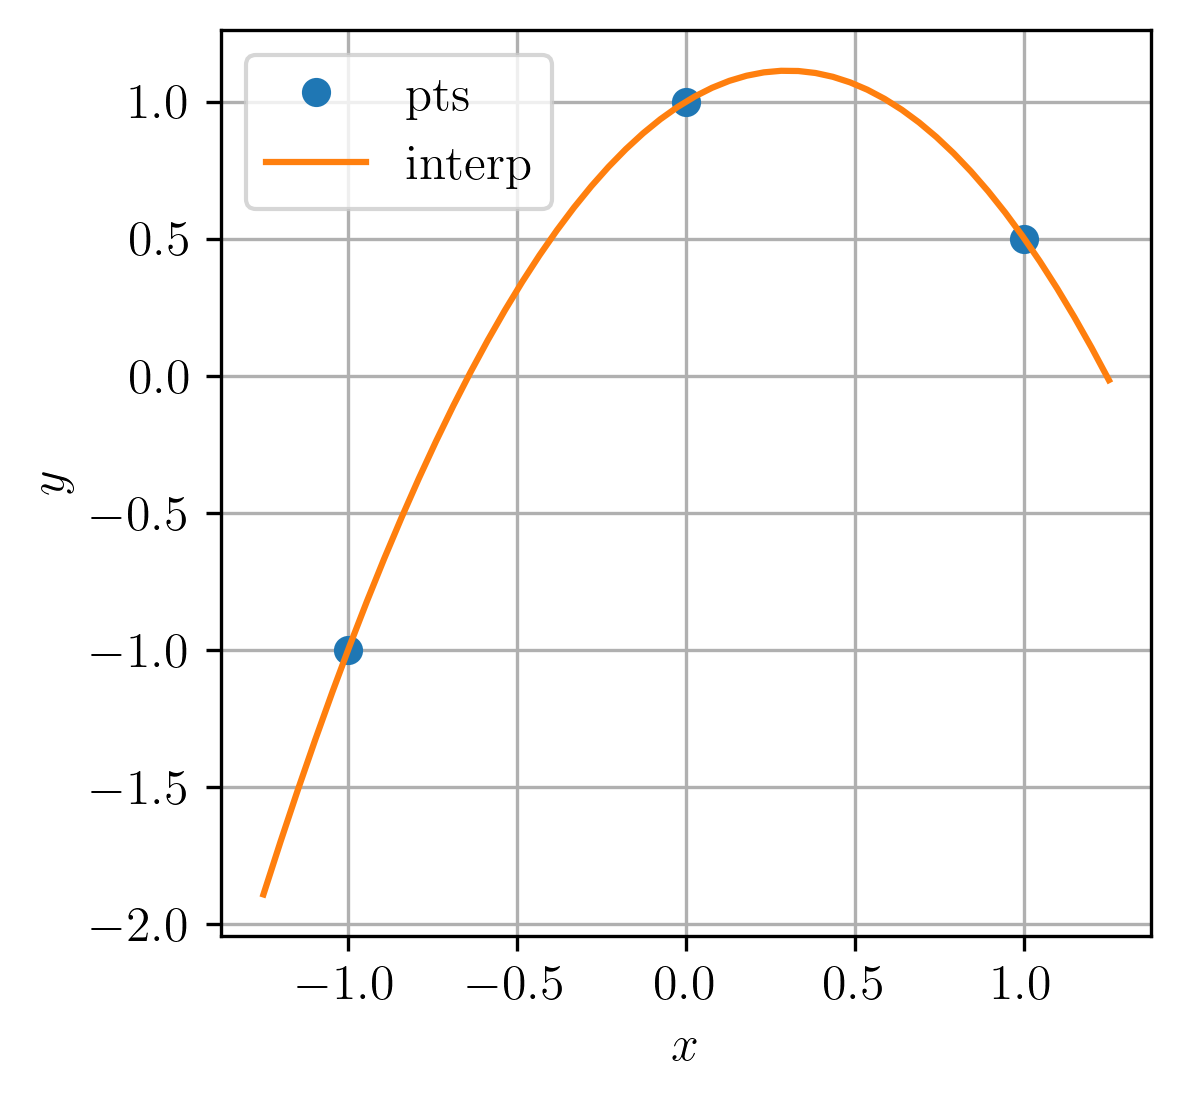
\includegraphics[width=3in]{./cap_interp/dados/fig_poliInterp/fig}
  \caption{Esboço do polinômio interpolador referente ao Exemplo \ref{cap_interp_sec_interpoli:ex:interpoli_intro}.}
  \label{cap_interp_sec_interpoli:fig:interpoli_intro}
\end{figure}

\begin{lstlisting}[caption=poliInterp.py]
import numpy as np
import numpy.linalg as npla

def poliInterp(x, y):
  # num. pts
  n = x.size
  # Vandermonde
  A = np.empty((n,n))
  for j in range(n):
    A[:,j] = x**(n-1-j)
  # coefs
  p = npla.solve(A, y)
  return p

# exemplo
x = np.array([-1., 0, 1])
y = np.array([-1., 1, 1/2])

# poli interp
p = poliInterp(x, y)

# verificação
print(np.polyval(p, x))
\end{lstlisting}

\end{ex}

\subsection{Exercícios}

\begin{exer}
  Obtenha o polinômio interpolador do conjunto de pontos 
  $\{(-1, -1)$, $(-0.5, 1)$, $(1, 2)\}$.
\end{exer}
\begin{resp}
  $$-1,\bar{6}x^2 + 1.5x + 2.1\bar{6}$$
\end{resp}

\begin{exer}
  Obtenha o polinômio interpolador do conjunto de pontos $\{(-1, -1)$, $(0, 1)$, $(1, 1/2)$, $(2, 1)\}$.
\end{exer}
\begin{resp}
  $$0.58\bar{3}x^3 - 1.25x^2 + 0.1\bar{6}x + 1$$. 
\end{resp}

\begin{exer}
  Obtenha o polinômio interpolador do conjunto de pontos $\{(-1,~-1)$, $(0, 1)$, $(1, 1/2)$, $(2, 1)$, $(2.5, 1)\}$.
\end{exer}
\begin{resp}
  $$-0.26190476x^4 + 1.10714286x^3 - 0.98809524x^2 - 0.35714286x  + 1$$.  
\end{resp}

\begin{exer}
  Considere a matriz de Vandermonde $V = [\pmb{x}^{n-j}]_{j=1}^{n}$, com $\pmb{x} = (x_1, x_2, \dotsc, x_n)$, sendo $x_i = (i-1)h$, $h=0.1$ e $i = 1, 2, \dotsc, n$. Compute o número de condicionamento de $V$ para $n=5, 10, 100$. De que forma os resultados obtidos impactam no problema de interpolação polinomial?
\end{exer}
\begin{resp}

  \begin{tabular}{rr}
    $n$ & $\kappa(V)$\\\midrule
    $5$ & $1.03\E+4$\\
    $10$ & $2.57\E+7$\\
    $100$ & $9.11\E+109$\\\bottomrule
  \end{tabular}

\end{resp}

\begin{exer}
  Aproxime a função $f(x) = \cos(x)$ por um polinômio interpolador $p$ no intervalo $[0, \pi]$. Escolhas pontos nesse intervalo de forma a obter $p$ que aproxime $f$ com boa precisão.
\end{exer}
\begin{resp}
  Dica: use os pontos $x_i = (i-1)\frac{\pi}{4}$, $i = 1, 2, 3, 4$.
\end{resp}

\ifisbook
\subsubsection{Respostas}
\shipoutAnswer
\fi

%%% SECTION %%%

\section{Interpolação de Lagrange}\label{cap_interp_sec_lagrange}

\hl{Interpolação de Lagrange{\lagrange} é uma técnica para a computação do polinômio interpolador $p(x)$ de um conjunto de pontos $\{(x_i, y_i)\}_{i=1}^n$ dados}. A ideia consiste em escrever o polinômio interpolador na forma
\begin{subequations}\hleq
  \begin{align}
    p(x) &= \sum_{i=1}^n y_iL_i(x)\\
         &= y_1L_1(x) + y_2L_2(x) + \cdots + y_nL_n(x),
  \end{align}
\end{subequations}
onde $L_i(x)$ é chamado de $i$-ésimo polinômio de Lagrange e é definido como o polinômio de grau $n-1$ que satisfaz
\begin{equation}\hleq
  L_i(x_j) = \left\{
    \begin{array}{ll}
      1 &, i=j\\
      0 &, i\neq j
    \end{array}
\right.
\end{equation}
Mais especificamente, temos que \hl{$L_i(x)$ tem raízes $\{x_1, \ldots, x_{i-1}, x_{i+1}, \ldots, x_n\}$} e, portanto, pode ser decomposto na forma
\begin{subequations}
  \begin{align}
    L_i(x) &= c_i\prod_{\overset{j=1}{j\neq i}}^n (x-x_j)\\
           &= c_i(x-x_1)\cdots(x-x_{i-1}) \nonumber\\
           &\quad \times (x-x_i)\cdots(x-x_n).
  \end{align}
\end{subequations}
Além disso, como $L_i(x_i) = 1$, temos
\begin{equation}
  c_i = \frac{1}{\displaystyle\prod_{\overset{j=1}{j\neq i}}^n (x_i-x_j)}.
\end{equation}
Assim sendo, podemos concluir que
\begin{subequations}\hleq
  \begin{align}
    L_i(x) &= \prod_{\overset{j=1}{j\neq i}}^n \frac{x-x_j}{x_i-x_j} \\
           &= \frac{(x-x_1)\cdots(x-x_{i-1})}{(x_i-x_1)\cdots(x_i-x_{i-1})} \nonumber \\
           &\quad \times \frac{(x-x_{i+1})\cdots(x-x_n)}{(x_i-x_{i+1})\cdots(x_i-x_n)}.
  \end{align}
\end{subequations}

\begin{ex}
  Consideramos o problema de encontrar o polinômio interpolador do conjunto de pontos $\{(-1, -1), (0, 1), (1, 1/2)\}$. Como temos 3 pontos, o polinômio tem grau 2 e pode ser escrito na seguinte forma de Lagrange
  \begin{equation}
    p(x) = y_1L_1(x) + y_2L_2(x) + y_3L_3(x),
  \end{equation}
  onde $y_1 = -1$, $y_2 = 1$ e $y_3 = 1/2$. Os polinômios de Lagrange são dados por
  \begin{align}
    L_1(x) &= \frac{(x-x_2)(x-x_3)}{(x_1-x_2)(x_1-x_3)} \\
           &= \frac{1}{2}x^2 - \frac{1}{2}x,\\
    L_2(x) &= \frac{(x-x_1)(x-x_3)}{(x_2-x_1)(x_2-x_3)} \\
           &= -x^2 + 1,\\
    L_3(x) &= \frac{(x-x_1)(x-x_2)}{(x_3-x_1)(x_3-x_2)} \\
           &= \frac{1}{2}x^2 + \frac{1}{2}x.\\
  \end{align}
  E, então, temos o polinômio interpolador
  \begin{equation}
    p(x) = -1.25x^2 + 0.75x + 1.
  \end{equation}

\begin{lstlisting}[caption=poliLagrange.py]
import numpy as np

def poliLagrange(xpts, ypts):
  # num. pts
  n = xpts.size
  # interp poli
  p = np.poly1d(0)
  for i in range(n):
    # Lagrange poli
    L = np.poly1d(1)
    for j in range(n):
      if (i != j):
        L *= np.poly1d([1, -xpts[j]])/(xpts[i]-xpts[j])
    p += ypts[i] * L
  return p



# exemplo
xpts = np.array([-1., 0, 1])
ypts = np.array([-1., 1, 1/2])


# interp poli
p = poliLagrange(xpts, ypts)
print(p)

# verificação
print(p(x))
\end{lstlisting}

\end{ex}

\subsection{Aproximação de Funções}

Polinômio interpoladores podem ser usados para a aproximação de funções. \hl{Podemos aproximar uma dada função $f$ pelo polinômio interpolador de um conjunto de pontos selecionados $\{(x_i, y_i=f(x_i))\}_{i=1}^n$}. De fato, o seguinte teorema nos fornece uma estimativa para o erro de uma tal interpolação.

\begin{teo}[\hl{Teorema de Lagrange}]\label{cap_interp_sec_lagrange:teo:lagrange}
  Sejam dados uma função $f\in C^{n+1}([a, b])$ e $n$ pontos $\{x_i\}_{i=1}^n\subset [a, b]$. Então, o polinômio interpolador do conjunto de pontos $\{x_i, y_i=f(x_i)\}_{i=1}^n$ satisfaz
  \begin{equation}\hleq
    f(x) = p(x) + \frac{f^{(n+1)}(\xi)}{(n+1)!}\prod_{i=1}^n(x-x_i).
  \end{equation}
\end{teo}

\begin{ex}\label{cap_interp_sec_lagrange:ex:interpoli_aprox}
  Consideramos o problema de aproximar $f(x) = \sen(x)$ pelo polinômio interpolador do conjunto de pontos $x_1=0$, $x_2=\pi/2$ e $x_3=\pi$. I.e., queremos determinar o polinômio $p(x)$ de grau $2$ que interpola os pontos $\{(0, 0),~(\pi/2, 1),~(\pi, 0)\}$. Usando a técnica de Lagrange, obtemos
  \begin{equation}
    p(x) = -0.41x^2 + 1.3x,
  \end{equation}
com seus coeficientes arredondados para dois dígitos significativos. A Figura \ref{cap_interp_sec_lagrange:fig:interpoli_aprox} mostra os esboços da função $f(x)=\sen(x)$, dos pontos dados e do polinômio interpolador $p(x)$.

\begin{figure}[H]
  \centering
  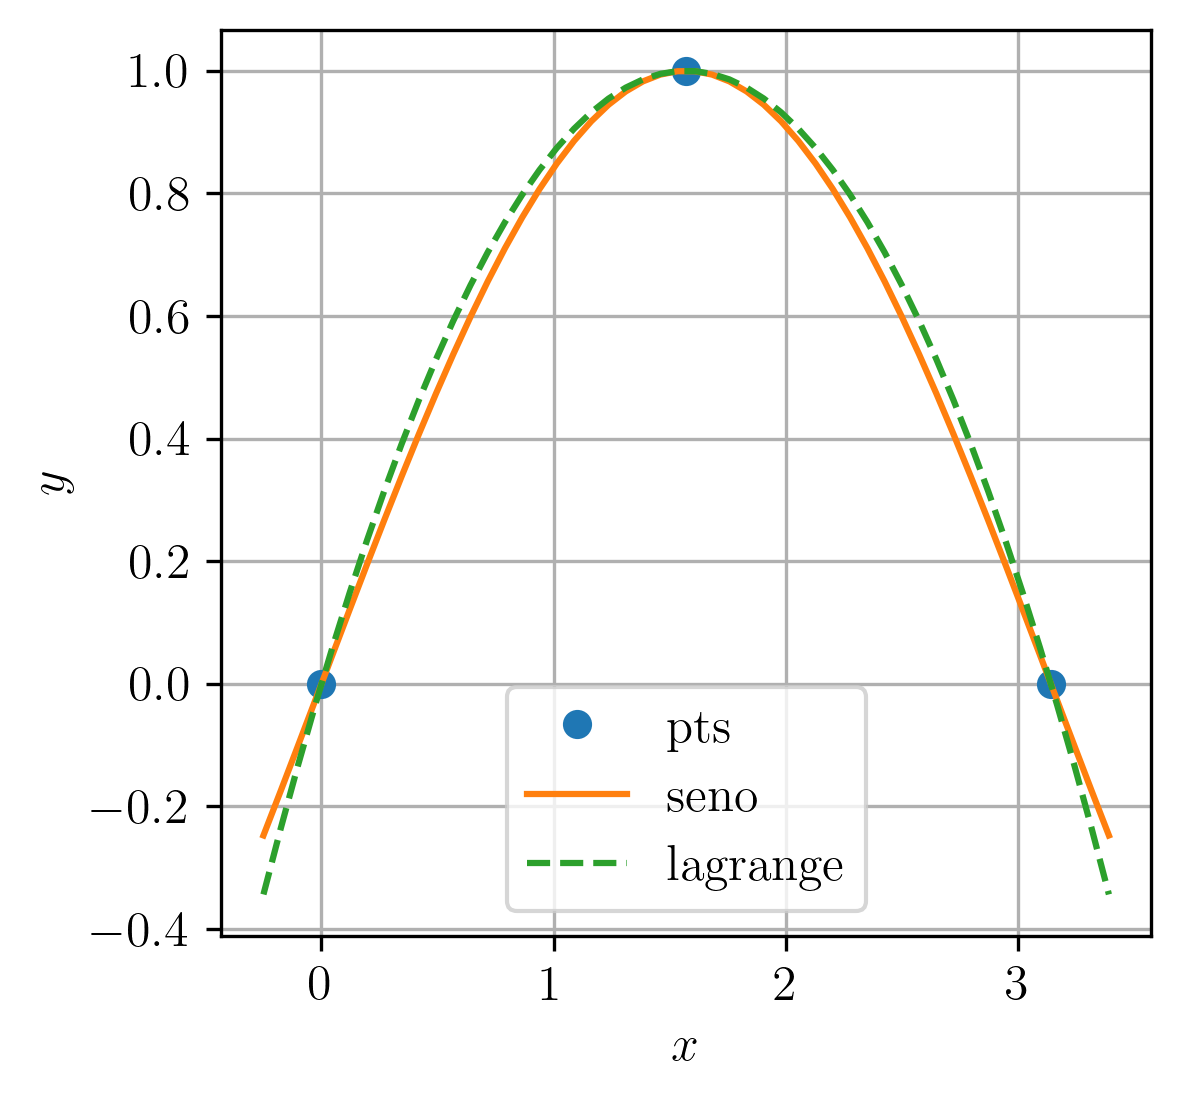
\includegraphics[width=0.7\textwidth]{./cap_interp/dados/fig_poliLagrange/fig}
  \caption{Esboços dos gráficos da função, dos pontos e do polinômio interpolador computado no Exemplo \ref{cap_interp_sec_lagrange:ex:interpoli_aprox}.}
  \label{cap_interp_sec_lagrange:fig:interpoli_aprox}
\end{figure}

\begin{lstlisting}
x = np.array([0, np.pi/2, np.pi])
f = lambda x: np.sin(x)
poli = poliLagrange(x, f(x))
\end{lstlisting}

\end{ex}

\subsection{Exercícios}

\begin{exer}
  Use a técnica de Lagrange para obter o polinômio interpolador do conjunto de pontos $\{(-1, -1)$, $(-0.5, 1)$, $(1, 2)\}$.
\end{exer}
\begin{resp}
  $-1,\bar{6}x^2 + 1.5x + 2.1\bar{6}$
\end{resp}

\begin{exer}
  Use a técnica de Lagrange para obter o polinômio interpolador do conjunto de pontos $\{(-1, -1)$, $(0, 1)$, $(1, 1/2)$, $(2, 1)\}$.
\end{exer}
\begin{resp}
  $0.58\bar{3}x^3 - 1.25x^2 + 0.1\bar{6}x + 1$. 
\end{resp}

\begin{exer}
  Use a técnica de Lagrange para obter o polinômio interpolador do conjunto de pontos $\{(-1, -1)$, $(0, 1)$, $(1, 1/2)$, $(2, 1)$, $(2.5, 1)\}$.
\end{exer}
\begin{resp}
  $-0.26190476x^4  1.10714286x^3 -0.98809524x^2 -0.35714286x  1$.  
\end{resp}

\begin{exer}
  Use a técnica de interpolação de Lagrange para encontrar o polinômio interpolador que aproxima a função$f(x)=e^{x}$ pelos pontos $x_1=0$, $x_2=1$, $x_3=1.5$ e $x_4=2$.
\end{exer}
\begin{resp}
$0.54x^3 - 0.15x^2 + 1.3x + 1$.
\end{resp}

\begin{exer}
  Use a técnica de Lagrange para aproximar a função $f(x) = \cos(x)$ por um polinômio interpolador $p$ no intervalo $[0, \pi]$. Escolha pontos de forma a obter $p$ que aproxime $f$ com boa precisão.
\end{exer}
\begin{resp}
  Dica: use os pontos $x_i = (i-1)\frac{\pi}{4}$, $i = 1, 2, 3, 4$.
\end{resp}

\ifisbook
\subsubsection{Respostas}
\shipoutAnswer
\fi

%%% SECTION %%%
\section{Diferenças Divididas de Newton}\label{cap_interp_sec_difdiv}

Dado um conjunto de pontos $\{(x_i, y_i)\}_{i=1}^n$, o \hl{\emph{Método das Diferenças Divididas de Newton}}{\newton} busca determinar o \hl{polinômio interpolador da forma}
\begin{equation}\hleq
  \begin{aligned}
    p(x) &= a_1 + a_2(x-x_1) \\
    &+ a_3(x-x_1)(x-x_2)\\
    &+ \cdots + a_{n}(x-x_1) \cdots (x-x_{n-1}).
  \end{aligned}
\end{equation}
Por uma abordagem direta, temos que $p(x_i)=y_i$, $i=1, 2, \dotsc, n$, o que nos leva ao seguinte sistema triangular inferior
\begin{subequations}
  \begin{align}
    a_1 &= y_1, \\
    a_1 + a_2(x_2-x_1) &= y_2, \\
    a_1 + a_2(x_3-x_1) + a_3(x_3-x_1)(x_3-x_2) &= y_3, \\
        &\vdots\\
    a_1 + a_2(x_n-x_1) + \cdots + a_{n}(x_n-x_1)\cdot\cdots\cdot(x_n-x_{n-1}) &= y_n.
  \end{align}
\end{subequations}
Entretanto, existe uma forma mais eficiente de se determinar os coeficientes $a_i$, $i=1, 2, \dotsc, n$.

Denotemos por $p[x_j, x_{j+1}, \dotsc, x_{k}](x)$ o polinômio interpolador do conjunto de pontos $\{(x_i, y_i)\}_{i=j}^k$. Então, temos a seguinte recursão
\begin{equation}\label{cap_interp_sec_difdiv:eq:interp_parc1}\hleq
  p[x_j] = y_j,
\end{equation}
para $j=1, 2, \dotsc, n$ e
\begin{equation}\label{cap_interp_sec_difdiv:eq:interp_parc2}\hleq
  \begin{aligned}
    &p[x_j, x_{j+1}, \ldots, x_k](x)\\
    &\quad = \frac{(x-x_j)p[x_{j+1},\dotsc,x_k](x)-(x-x_k)p[x_j,\dotsc,x_{k-1}](x)}{x_k-x_j},
  \end{aligned}
\end{equation}
para todo $n\geq k > j \geq 1$.

De fato, \eqref{cap_interp_sec_difdiv:eq:interp_parc1} é trivial. Agora, denotando por $r(x)$ o lado direito da equação \eqref{cap_interp_sec_difdiv:eq:interp_parc2}, vemos que $r(x)$ tem grau menor ou igual a $k-j$, o mesmo de $p[x_j, x_{j+1}, \ldots, x_k](x)$. Desta forma, para mostrar \eqref{cap_interp_sec_difdiv:eq:interp_parc2}, basta verificarmos que $r(x)$ interpola o conjunto de pontos $\{(x_i, y_i)\}_{i=j}^k$. O que de fato ocorre
\begin{subequations}
  \begin{align}
    &r(x_j) = \frac{-(x_j-x_k)y_j}{x_k-x_j} = y_j,\\
    &r(x_{l}) = \frac{(x_l-x_j)y_l-(x_l-x_k)y_l}{x_k-x_j}=y_l,\nonumber\\
    &\qquad\qquad\qquad\qquad l=j+1,\dotsc,k-1,\\
    &r(x_k) = \frac{(x_k-x_j)y_k}{x_k-x_j}=y_k.
  \end{align}
\end{subequations}
Logo, pela unicidade do polinômio interpolador\endnote{Consulte o Exercício \ref{cap_interp_sec_difdiv:exer:pinterp_unico}}, temos demonstrado \eqref{cap_interp_sec_difdiv:eq:interp_parc2}.

Observando que o polinômio interpolador $p(x)$ é igual a $p[x_1,\dotsc,x_n](x)$, temos que \eqref{cap_interp_sec_difdiv:eq:interp_parc1}-\eqref{cap_interp_sec_difdiv:eq:interp_parc2} nos fornece uma forma de computar $p(x)$ de forma recursiva. Além disso, observemos que $p[x_j, \dotsc, x_{k-1}](x)$ e $p[x_j, \dotsc, x_k]$ diferem por um polinômio de grau $k-j$ com zeros $x_j$, $x_{j+1}$, ..., $x_{k-1}$. Logo, temos
\begin{equation}
  \begin{aligned}
    &p[x_j,\dotsc,x_k](x) = p[x_j,\dotsc,x_{k-1}](x) \\
    &\qquad + f[x_j,\dotsc,x_k](x-x_j)\cdots(x-x_{k-1}),
  \end{aligned}
\end{equation}
onde $f[x_j, \dotsc, x_k]$ são coeficientes a determinar. Ainda, tomando $p[x_i] = f[x_i]$, temos
\begin{equation}
  \begin{aligned}
    &p[x_j,\dotsc,x_k](x) = f[x_j] + f[x_j,x_{j+1}](x-x_j)\\
    &\qquad + f[x_j,\dotsc,x_k](x-x_j)\cdots(x-x_{k-1}).
  \end{aligned}
\end{equation}
Por fim, a recursão \eqref{cap_interp_sec_difdiv:eq:interp_parc1}-\eqref{cap_interp_sec_difdiv:eq:interp_parc2} nos mostra que as \hl{Diferenças Divididas Newton podem ser obtidas de}
\begin{subequations}\label{cap_interp_sec_difdiv:eq:interp_difdiv}\hleq
  \begin{align}
    &f[x_j] = y_j,\quad j = 1, 2, \dotsc, n,\\
    &f[x_j,\dotsc,x_k] = \frac{f[x_{j+1},\dotsc,x_k]-f[x_j,\dotsc,x_{k-1}]}{x_k-x_j},
  \end{align}
\end{subequations}
para todo $n\geq k > j \geq 1$. E, temos \hl{o polinômio interpolador} do conjunto de pontos $\{(x_i,y_i)\}_{i=1}^n$ dado por
\begin{equation}\label{cap_interp_sec_difdiv:eq:interpoli_Newton}\hleq
  \begin{aligned}
    &p[x_1,\dotsc,x_n](x) = f[x_1] + f[x_1,x_2](x-x_1) \\
    &\qquad + \cdots + f[x_1,\dotsc,x_n](x-x_1)\cdots(x-x_n).  
  \end{aligned}
\end{equation}

\begin{obs}
  A recursão \eqref{cap_interp_sec_difdiv:eq:interp_difdiv} pode ser adequadamente organizada em uma matriz da forma
  \begin{equation}
    \begin{bmatrix}
      \pmb{f[x_1]} & 0 & 0 & \ldots & 0 \\
      f[x_2] & \pmb{f[x_1,x_2]} & 0 & \ldots & 0 \\
      f[x_3] & f[x_2,x_3] & \pmb{f[x_1,x_2,x_3]} & \ldots & 0\\
      \vdots & \vdots & \vdots & \ldots & \vdots \\
      f[x_n] & f[x_{n-1},x_{n}] & f[x_{n-2},x_{n-1},x_n] & \ldots & \pmb{f[x_1,x_2,\dotsc,x_n]}
    \end{bmatrix}
  \end{equation}
onde \hl{os elementos da diagonal correspondem aos coeficientes do polinômio interpolador na forma {\eqref{cap_interp_sec_difdiv:eq:interpoli_Newton}}}.
\end{obs}


\begin{ex}
  Consideramos o problema de encontrar o polinômio interpolador do conjunto de pontos $\{(-1, -1), (0, 1), (1, 1/2)\}$. Usando o Método das Diferenças Divididas de Newton, escrevemos o polinômio na forma
  \begin{equation}
    p(x) = f[x_1] + f[x_1,x_2](x-x_1) + f[x_1,x_2,x_3](x-x_1)(x-x_2).
  \end{equation}
  Então, computamos seus coeficientes pela recursão \eqref{cap_interp_sec_difdiv:eq:interp_difdiv}. Ou seja, temos
  \begin{subequations}
    \begin{align}
      &f[x_1] = -1,\\
      &f[x_2] = 1,\\
      &f[x_3] = 1/2.
  \end{align}
  \end{subequations}
  Daí, segue
  \begin{subequations}
    \begin{align}
      &f[x_1,x_2] = \frac{f[x_2]-f[x_1]}{x_2-x_1} = 2\\
      &f[x_2,x_3] = \frac{f[x_3]-f[x_2]}{x_3-x_2} = -\frac{1}{2}\\
    \end{align}
  \end{subequations}
  e, por fim, que
  \begin{subequations}
    \begin{align}
      &f[x_1,x_2,x_3] = \frac{f[x_2,x_3]-f[x_1,x_2]}{x_3-x_1}\\
      &\qquad\quad = -1.25.
    \end{align}
  \end{subequations}
  Logo, o polinômio interpolador é
  \begin{equation}
    p(x) = 0.5 + 2(x+1) - 1.25(x+1)(x-1),
  \end{equation}
  ou, equivalentemente,
  \begin{equation}
    p(x) = -1.25x^2 + 0.75x + 1.
  \end{equation}

\begin{lstlisting}
import numpy as np

def interpDDF(x, y):
  n = x.size
  M = np.empty((n,n))
  M[:,0] = y
  for j in range(1,n):
    for i in range(j,n):
      M[i,j] = (M[i,j-1] - M[i-1,j-1]) \
          / (x[i]-x[i-j])
  return np.diag(M)

def poliDDF(x, p, xpts):
  n = p.size
  pval = p[0]
  aux = 1.
  for i in range(1,n):
    aux *= (x-xpts[i-1])
    pval += p[i]*aux
  return pval

xpts = np.array([-1., 0, 1])
ypts = np.array([-1., 1, 1/2])
p = interpDDF(xpts, ypts)
print(poliDDF(xpts, p, xpts))
\end{lstlisting}

\end{ex}

\subsection{Exercícios}

\begin{exer}
  Use o Método das Diferenças Divididas de Newton para obter o polinômio interpolador do conjunto de pontos $\{(-1, -1), (-0.5, 1), (1, 2)\}$.
\end{exer}
\begin{resp}
  $-1,\bar{6}x^2 + 1.5x + 2.1\bar{6}$
\end{resp}

\begin{exer}
  Use o Método das Diferenças Divididas de Newton para obter o polinômio interpolador do conjunto de pontos $\{(-1, -1), (0, 1), (1, 1/2), (2, 1)\}$.
\end{exer}
\begin{resp}
  $0.58\bar{3}x^3 - 1.25x^2 + 0.1\bar{6}x + 1$. 
\end{resp}

\begin{exer}
  Use o Método das Diferenças Divididas de Newton para obter o polinômio interpolador do conjunto de pontos $\{(-1, -1), (0, 1), (1, 1/2), (2, 1), (2.5, 1)\}$.
\end{exer}
\begin{resp}
  $-0.26190476x^4  1.10714286x^3 -0.98809524x^2 -0.35714286x  1$.  
\end{resp}

\begin{exer}
  Use o método das diferenças divididas de Newton para encontrar o polinômio interpolador que aproxima a função $f(x)=e^{x}$ pelos pontos $x_1=0$, $x_2=1$, $x_3=1.5$ e $x_4=2$.
\end{exer}
\begin{resp}
$p(x) = 0.54x^3 - 0.15x^2 + 1.3x + 1$.
\end{resp}

\subsubsection{Análise Numérica}

\begin{exer}\label{cap_interp_sec_difdiv:exer:pinterp_unico}
  Dado um conjunto de pontos distintos $\{(x_i, y_i)\}_{i=1}^n$, mostre que é único o polinômio interpolador do conjunto.
\end{exer}

\ifisbook
\subsubsection{Respostas}
\shipoutAnswer
\fi

%%% SECTION %%%

\section{Spline Cúbico}\label{cap_interp_sec_splines}

\hl{Dado um conjunto de pontos $\{(x_i,y_i)\}_{i=1}^n$, um \emph{spline cúbico} é uma função duas vezes continuamente diferenciável da forma}
\begin{equation}\hleq
  \begin{small}
    s(x)\!=\!\left\{
      \begin{array}{ll}
        \!s_{11}(x-x_1)^3 + s_{12}(x-x_1)^2 + s_{13}(x-x_1) + s_{14} &,x_1\!\leq\!x\!<\!x_2,\\
        \!s_{21}(x-x_2)^3 + s_{22}(x-x_2)^2 + s_{23}(x-x_2) + s_{24} &,x_2\!\leq\!x\!<\!x_3,\\
                                                                   &, \vdots \\
        \!s_{n-1,1}(x-x_2)^3\!+\!s_{n-1,2}(x-x_2)^2\!+\!s_{n-1,3}(x-x_2)\!+\!s_{n-1,4}\!&,x_{n-1}\!\leq\!x\!\leq\!x_n.
      \end{array}
    \right.
  \end{small}
\end{equation}
que satisfaz as seguintes propriedades
\begin{enumerate}
\item \hl{$s(x_i) = y_i$} para $i=1, 2, \dotsc, n$,
\item \hl{$s_j(x_j) = s_{j+1}(x_j)$} para todo $j = 1, 2, \dotsc, n-2$,
\item \hl{$s_j'(x_j) = s_{j+1}'(x_j)$} para todo $j = 1, 2, \dotsc, n-2$,  
\item \hl{$s_j''(x_j) = s_{j+1}''(x_j)$} para todo $j= 1, 2, \dotsc, n-2$.
\end{enumerate}

Observemos que o spline tem $4(n-1)$ coeficientes a determinar, enquanto que as condições acima nos fornecem $4n-6$ equações. Assim sendo, notamos que a determinação de \hl{um spline requer ainda 2 condições de fechamento}. Conforme a escolha destas condições, diferentes splines cúbicos são computados.

\subsection{Spline {\it Not-a-Knot}}

\hl{A condição \textit{not-a-knot} exige que o spline cúbico tenha derivada terceira contínua nos pontos $x_2$ e $x_{n-1}$}, i.e.
\begin{subequations}\hleq
  \begin{align}
    &s_1'''(x_2) = s_2'''(x_2),\\
    &s_{n-2}'''(x_{n-1}) = s_{n-1}'''(x_{n-1}).
  \end{align}
\end{subequations}

\begin{ex}\label{cap_interp_sec_splines:ex:interp_spline_nak}
  Consideremos o problema de aproximar a função $f(x)=\sen(x)$ pelo spline cúbico {\it not-a-knot} com pontos $x_1=0$, $x_2=\pi/6$, $x_3=\pi/3$ e $x_4=\pi/2$. Na Figura \ref{cap_interp_sec_splines:fig:interp_spline_nak} temos os esboços de $f$ e do spline cúbico computado. O spline computado é aproximadamente
  \begin{equation}
    s(x) = \small\left\{\begin{array}{ll}
                          -0.11x^3 - 0.11x^2 - 0.11x &, 0\leq x < \frac{\pi}{6}\\
                          -0.07(x-\frac{\pi}{6})^3 - 0.24(x-\frac{\pi}{6})^2 - 0.42(x-\frac{\pi}{6}) + \frac{1}{2} &, \frac{\pi}{6} \leq x < \frac{\pi}{3},\\
                          1.02(x-\frac{\pi}{3})^3 + 0.86(x-\frac{\pi}{3})^2 + 0.51(x-\frac{\pi}{3}) + \frac{\sqrt{3}}{2} &, \frac{\pi}{3} \leq x < \frac{\pi}{2}x
                                                                                                                     
    \end{array}\right.
  \end{equation}

  \begin{figure}[H]
    \centering
    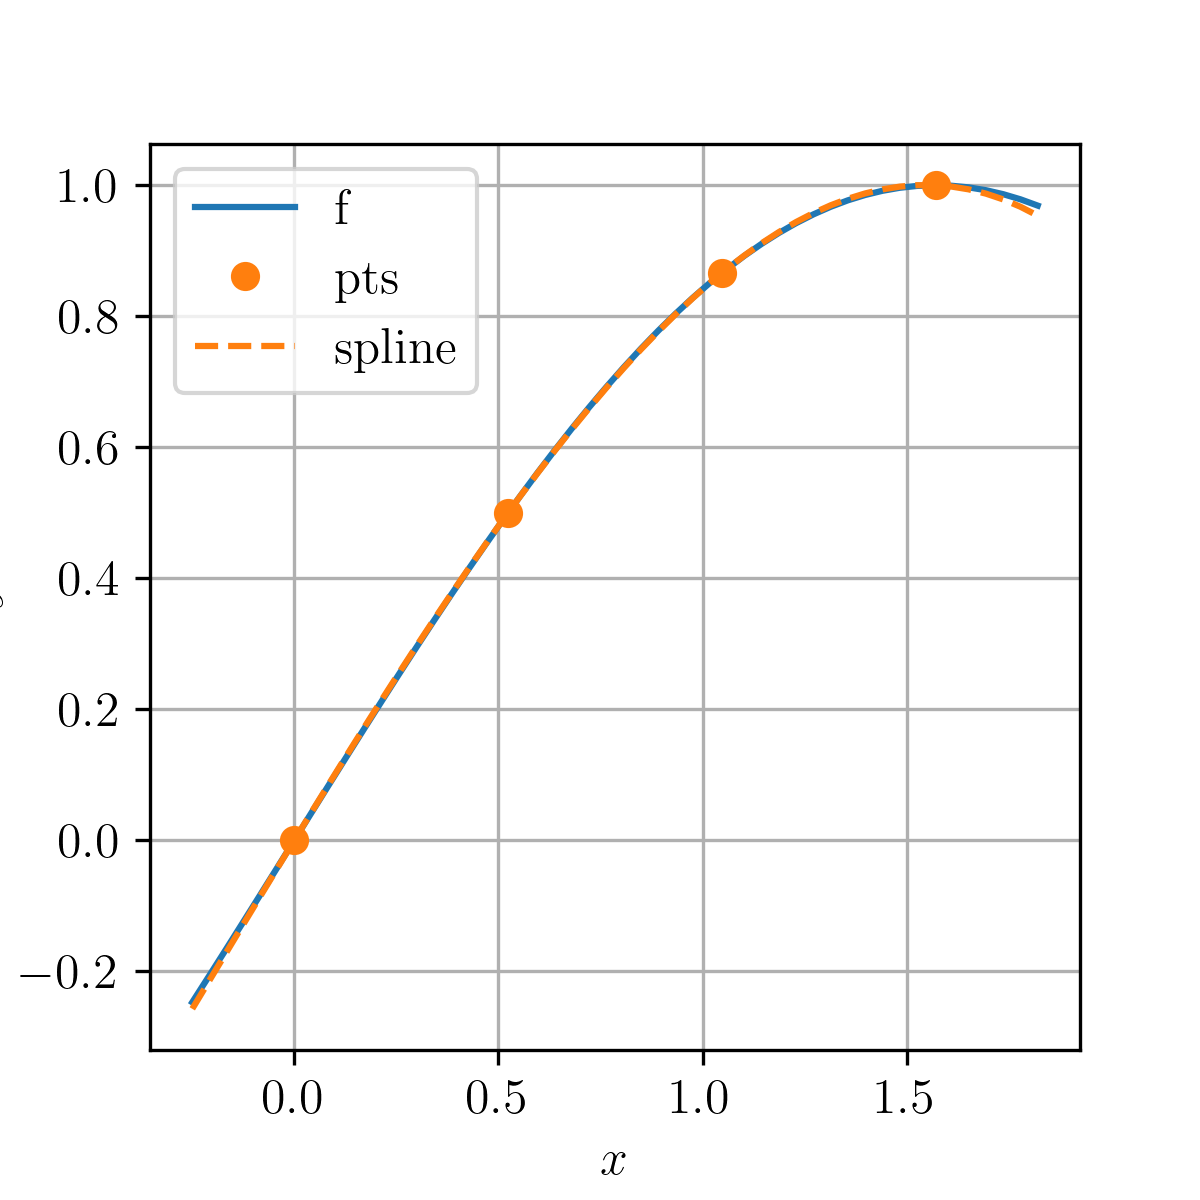
\includegraphics[width=0.8\textwidth]{./cap_interp/dados/fig_CSNotAKnot/fig}
    \caption{Esboço dos gráficos da função $f(x)=\sen(x)$ e do spline cúbico computado no Exemplo \ref{cap_interp_sec_splines:ex:interp_spline_nak}.}
    \label{cap_interp_sec_splines:fig:interp_spline_nak}
  \end{figure}

\begin{lstlisting}[caption=splineNotAKnot.py]
import numpy as np
from scipy.interpolate import CubicSpline

# dados
f = lambda x: np.sin(x)
xx = np.array([0.,
              np.pi/6,
              np.pi/3,
              np.pi/2])
yy = f(xx)

# spline
cs = CubicSpline(xx, yy)

# coefs
print(cs.c)
\end{lstlisting}

\end{ex}

\subsection{Spline Fixado}

Os \hl{splines cúbicos fixados são obtidos impondo os valores das derivadas na fronteira}, i.e.
\begin{subequations}\hleq
  \begin{align}
    &s'(x_1)=y_1',\\
    &s'(x_n)=y_n',
  \end{align}
\end{subequations}
onde $y_1'$ e $y_n'$ são escalares dados. Quando usamos splines para aproximarmos uma dada função $f$, usualmente, escolhemos $y_1'=f'(x_1)$ e $y_n'=f'(x_n)$.

\begin{ex}\label{cap_interp_sec_splines:ex:interp_spline_fixado}
  Consideremos o problema de aproximar a função $f(x)=\sen(x)$ pelo spline cúbico fixado com pontos $x_1=0$, $x_2=\pi/6$, $x_3=\pi/3$ e $x_4=\pi/2$. Na Figura \ref{cap_interp_sec_splines:fig:interp_spline_fixado} temos os esboços de $f$ e do spline cúbico computado
  \begin{equation}
    s(x) = \small\left\{
      \begin{array}{ll}
        -0.16x^3 - 0.12x^2 - 0.04x &, 0\leq x < \frac{\pi}{6}\\
        -0.001(x-\frac{\pi}{6})^3 - 0.26(x-\frac{\pi}{6})^2 - 0.44(x-\frac{\pi}{6}) + \frac{1}{2} &, \frac{\pi}{6} \leq x < \frac{\pi}{3},\\
        0.0(x-\frac{\pi}{3})^3 + 0.5(x-\frac{\pi}{3})^2 + 0.87(x-\frac{\pi}{3}) + \frac{\sqrt{3}}{2} &, \frac{\pi}{3} \leq x < \frac{\pi}{2}x
      \end{array}
\right.
  \end{equation}

  \begin{figure}[H]
    \centering
    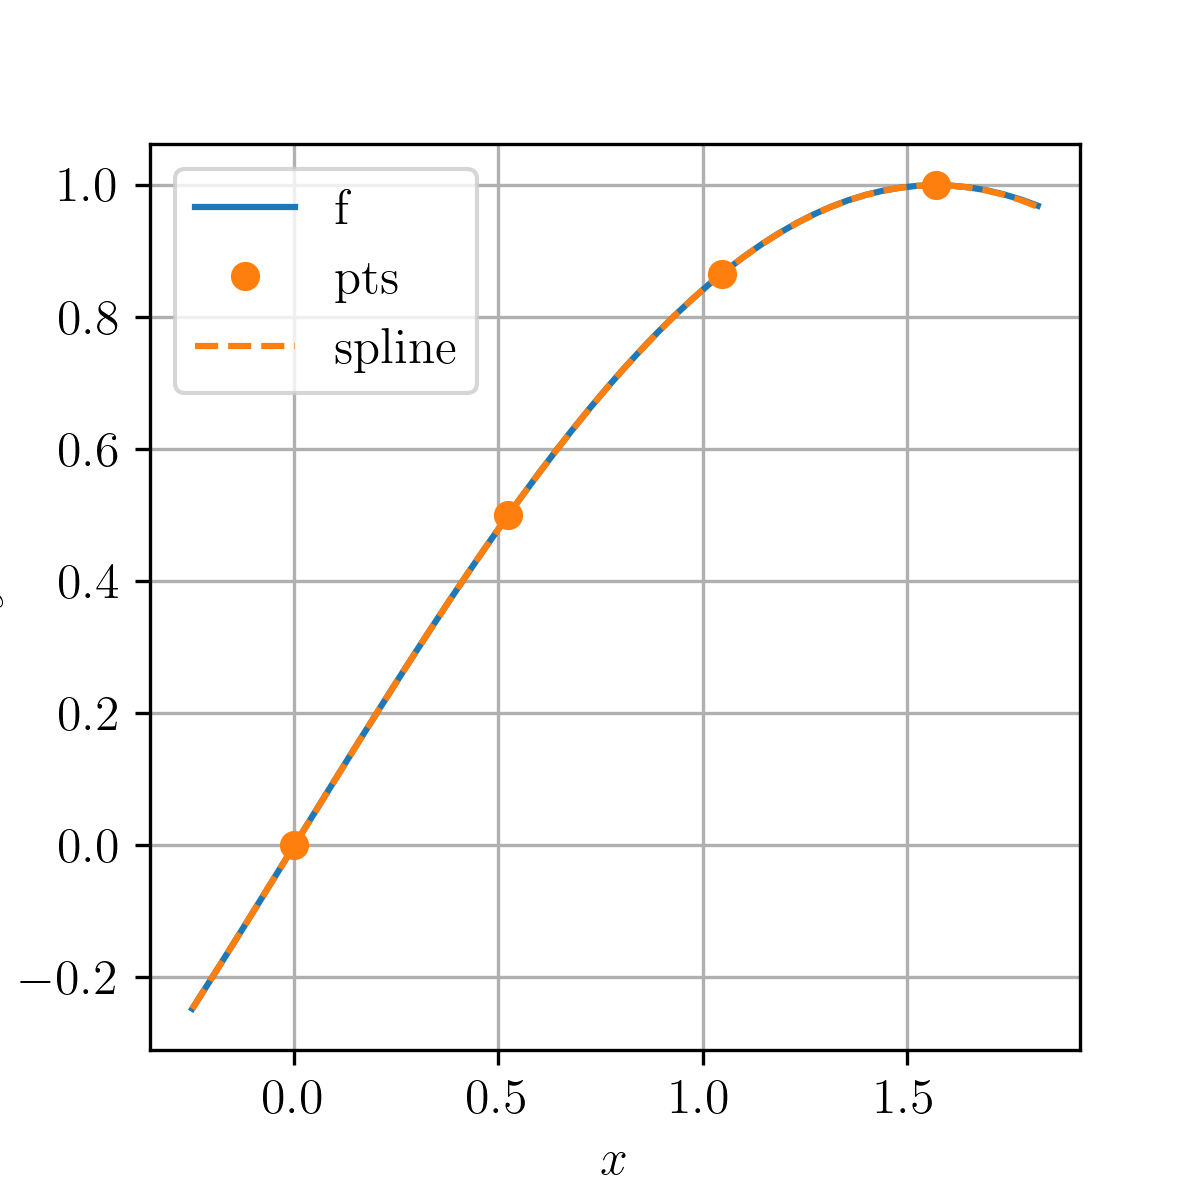
\includegraphics[width=0.8\textwidth]{./cap_interp/dados/fig_CSFixado/fig}
    \caption{Esboço dos gráficos da função $f(x)=\sen(x)$ e do spline cúbico fixado computado no Exemplo \ref{cap_interp_sec_splines:ex:interp_spline_fixado}.}
    \label{cap_interp_sec_splines:fig:interp_spline_fixado}
  \end{figure}

\begin{lstlisting}
import numpy as np
from scipy.interpolate import CubicSpline

# dados
f = lambda x: np.sin(x)
xx = np.array([0.,
              np.pi/6,
              np.pi/3,
              np.pi/2])
yy = f(xx)

# spline
cs = CubicSpline(xx, yy,
                 bc_type=((1, 1.),
                          (1, 0.)))

# coefs
print(cs.c)
\end{lstlisting}

\end{ex}

\subsection{Exercícios}

\begin{exer}
  Dado o conjunto de pontos $\{(-1, -1), (-0.5, 1), (1, 2)\}$, obtenha o spline cúbico associado com condição de controno:
  \begin{enumerate}[a)]
  \item Not-a-Knot.
  \item Fixado.
  \end{enumerate}
\end{exer}

\begin{exer}
  Dado o conjunto de pontos $\{(-1, -1), (0, 1), (1, 1/2), (2, 1)\}$, obtenha o spline cúbico associado com condição de controno:
  \begin{enumerate}[a)]
  \item Not-a-Knot.
  \item Fixado.
  \end{enumerate}
\end{exer}

\begin{exer}
  Dado o conjunto de pontos $\{(-1,~-1), (0, 1), (1, 1/2), (2, 1), (2.5, 1)\}$, obtenha o spline cúbico associado com condição de controno:
  \begin{enumerate}[a)]
  \item Not-a-Knot.
  \item Fixado.
  \end{enumerate}
\end{exer}

\begin{exer}
  Aproxime a função $f(x)=e^{x}$ por um spline cúbico que passa pelos pontos $x_1=0$, $x_2=1$, $x_3=1.5$ e $x_4=2$.
\end{exer}
\begin{resp}
  Dica: use um spline fixado.
\end{resp}

\begin{exer}
  Considere o problema de aproximar a função $f(x) = \cos(x)$ por um spline cúbico $s = s(x)$ no intervalo $[0, \pi]$. Escolha os pontos e a condição de fronteira de forma a obter $s$ que aproxime $f$ com boa precisão gráfica.
\end{exer}
\begin{resp}
  Dica: use um spline fixado.
\end{resp}

\ifisbook
\subsubsection{Respostas}
\shipoutAnswer
\fi

%%% SECTION %%%

\chapter{Aproximação por Mínimos Quadrados}\label{cap_ajuste}

\section{Problemas Lineares}\label{cap_ajuste_sec_prob_lin}

Dado um conjunto de $n$ pontos $\{(x_i,y_i)\}_{i=1}^n$, $x_i\neq x_j$ para $i\neq j$, e uma família de $m \leq n$ funções $\{f_i(x)\}_{i=1}^m$, \hl{o problema linear de \emph{aproximação por mínimos quadrados} consiste em determinar os $m$ coeficientes $\{c_i\}_{i=1}^m$ tal que a função}
\begin{align}
    &\hleq f(x; \pmb{c}) = \sum_{j=1}^m c_jf_j(x) \\
    & \text{}\qquad = c_1f_1(x) + c_2f_2(x) + c_3f_3(x) + \cdots + c_mf_m(x)
\end{align}
\hl{aproxime o dado conjunto de pontos no sentido de mínimos quadrados}, i.e. o \emph{vetor dos coeficientes} $\pmb{c} = (c_1, c_2, \dotsc, c_m)$ é solução do seguinte problema linear de minimização
\begin{equation}\hleq
  \min_{\pmb{c}} \left\{E:= \sum_{i=1}^n \left|y_i - f(x_i; \pmb{c})\right|^2\right\}.
\end{equation}

A fim de trabalharmos com uma notação mais compacta, definimos o \hlemph{resíduo} $\pmb{r}(\pmb{c}) = (r_1(\pmb{c}), r_2(\pmb{c}), \dotsc, r_n(\pmb{c}))$, onde $\hleq r_i(\pmb{c}) := y_i - f(x_i; \pmb{c})$. Com esta notação, \hl{o \emph{problema de mínimos quadrados}} se resume a resolver
\begin{equation}\label{cap_ajuste_sec_prob_lin:eq:pmq}\hleq
  \min_{\emph{c}} \{E := \left\|r(\pmb{c})\right\|^2\}.
\end{equation}

\subsection{Método das Equações Normais}

A fim de \hl{resolver o problema de mínimos quadrados} \eqref{cap_ajuste_sec_prob_lin:eq:pmq}, observamos que o \emph{erro quadrático}
\begin{align}
  & E := \left\|\pmb{r}(\pmb{c})\right\|_2^2 = \sum_{i=1}^n r_i^2(\pmb{c}) \\
  & \text{}\quad = \sum_{i=1}^n \left(y_i - f(x_i; \pmb{c})\right)^2 \\
  & \text{}\quad = \sum_{i=1}^n \left(y_i - \sum_{j=1}^m c_jf_j(x_i)\right)^2 \\
  & \hleq E = \|\pmb{y} - A\pmb{c}\|^2,
\end{align}
onde $\pmb{y} := (y_1, y_2, \dotsc, y_n)$ e
\begin{equation}\hleq
  A :=
  \begin{bmatrix}
    f_1(x_1) & f_2(x_1) & \cdots & f_m(x_1) \\
    f_1(x_2) & f_2(x_2) & \cdots & f_m(x_2) \\
    \vdots & \vdots & \vdots & \vdots \\
    f_1(x_n) & f_2(x_n) & \cdots & f_m(x_n)
  \end{bmatrix}.
\end{equation}

\hl{Os parâmetros $c_j$ que minimizam o erro $E$ são solução do seguinte sistema de equações}
\begin{equation}
  \frac{\p E}{\p c_j} = 2\sum_{i=0}^n r_i(c)\frac{\p}{\p c_j}r_i(c) = 0,
\end{equation}
onde $j=1, 2, \dotsc, m$. Ou, em uma notação mais apropriada,
\begin{align}
  & \nabla_{\pmb{c}} E = 0\\
  & -A^T\pmb{r}(\pmb{c}) = 0\\
  & -A^T(\pmb{y} - A\pmb{c}) = 0\\
  & A^TA\pmb{c} = A^T\pmb{y}.
\end{align}
Portanto, \hl{o problema linear de mínimos quadrados se resume em resolver as} chamadas \hl{\emph{equações normais}}
\begin{equation}\label{cap_ajuste_sec_prob_lin:eq:equacoes_normais}\hleq
  A^TA\pmb{c}= A^T\pmb{y}.
\end{equation}
Concluímos que a solução é dada por
\begin{equation}
  \pmb{c} = \left(A^TA\right)^{-1}A^T\pmb{y},
\end{equation}
quando $A^TA$ é inversível.

\begin{ex}[\hl{Ajuste de Polinômios}]\label{cap_ajuste_sec_prob_lin:ex:ajuste_de_polinomios}
  Considere o problema de ajustar o conjunto de pontos
  \begin{center}
    \begin{tabular}{lrr}
      $i$ & $x_i$ & $y_i$ \\\midrule
      $1$ & $-1.0$ &  $1.2$ \\
      $2$ &  $0.0$ & $-0.1$ \\
      $3$ &  $1.0$ &  $0.7$ \\
      $4$ &  $1.5$ &  $2.4$ \\\bottomrule
    \end{tabular}
  \end{center}
  por um polinômio quadrático
  \begin{equation}
    p(x) = p_1x^2 + p_2x + p_3
  \end{equation}
  no sentido de mínimos quadrados.  

  \begin{figure}[htb]
    \centering
    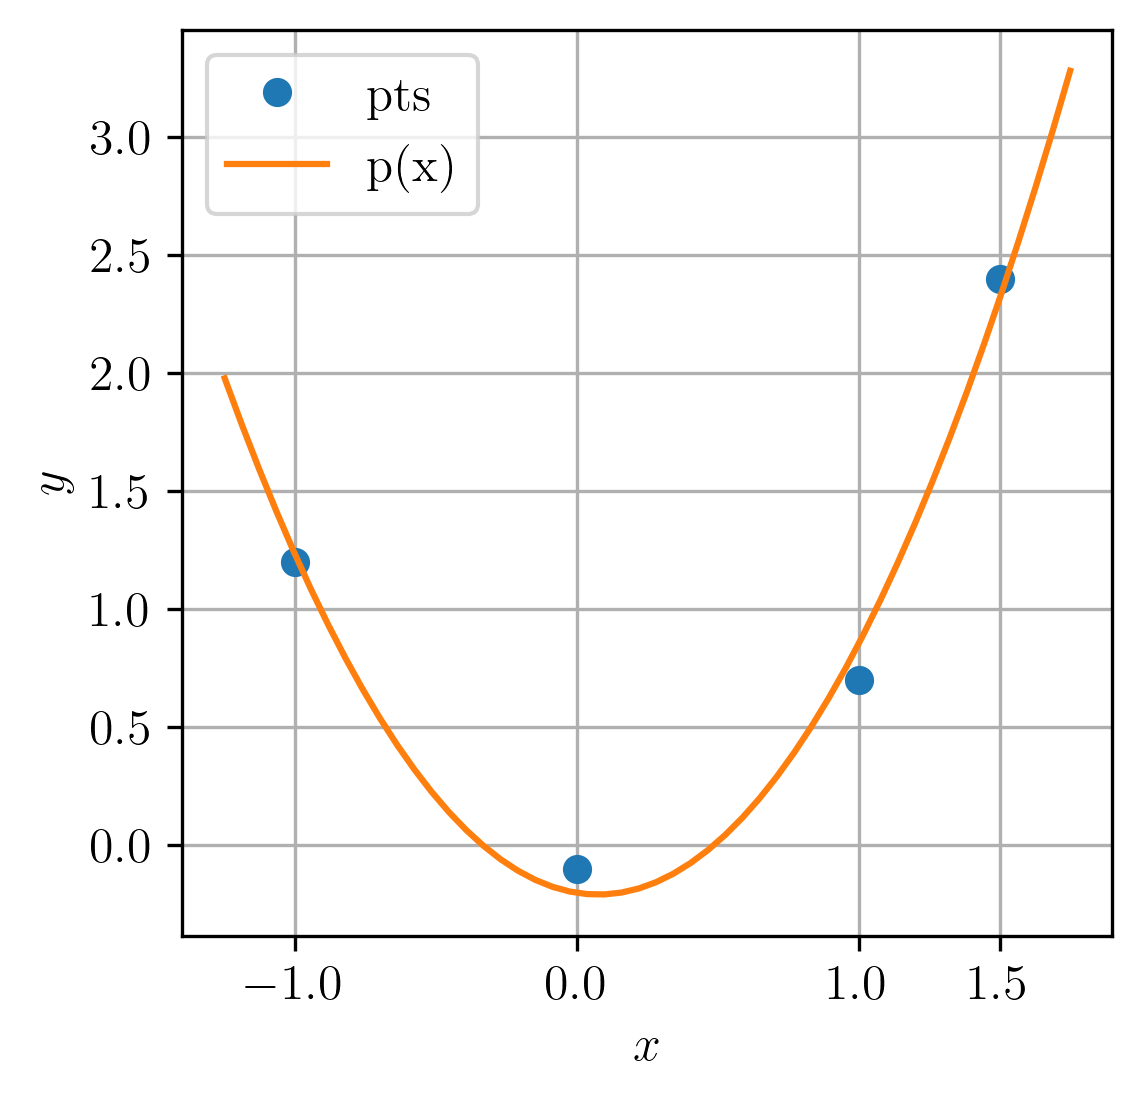
\includegraphics[width=4in]{cap_ajuste/dados/fig_mqPoli/fig.png}
    \caption{Polinômio ajustado no Exemplo~\ref{cap_ajuste_sec_prob_lin:ex:ajuste_de_polinomios}.}
    \label{cap_ajuste_sec_prob_lin:fig:ex_mq_poli}
  \end{figure}
  
  Neste caso, a família de funções do problema de mínimos quadrados é $f_1(x) = x^2$, $f_2(x) = x$ e $f_3(x) = 1$. Assim sendo, os coeficientes $p = (p_1, p_2, p_3)$ são solução do seguinte sistema linear
  \begin{equation}\label{cap_ajuste_sec_prob_lin:eq:aux3_md}
    A^TA\pmb{p} = A^T\pmb{y},
  \end{equation}
  onde $\pmb{y} = (y_1, y_2, y_3)$ e
  \begin{equation}
    A :=
    \begin{bmatrix}
      x_1^2 & x_1 & 1 \\
      x_2^2 & x_2 & 1 \\
      x_3^2 & x_3 & 1 \\
      x_4^2 & x_4 & 1
    \end{bmatrix}.
  \end{equation}
  Emfim, resolvendo as equações normais~\eqref{cap_ajuste_sec_prob_lin:eq:aux3_md}, obtemos
  \begin{equation}
    p(x) = 1.25x^2 -0.188x - 0.203.
  \end{equation}
  A Figura~\ref{cap_ajuste_sec_prob_lin:fig:ex_mq_poli} mostra um esboço dos pontos e do polinômio ajustado.

\begin{lstlisting}[caption=mqPoli.py]
import numpy as np
import numpy.linalg as npla

# dados
xx = np.array([-1.0, 0.0, 1.0, 1.5])
yy = np.array([1.2, -0.1, 0.7, 2.4])

# matriz
m = 3
n = xx.size
A = np.empty((n,m))
A[:,0] = xx**2
A[:,1] = xx
A[:,2] = np.ones_like(xx)

# sol de mq
p = npla.solve(A.T@A, A.T@yy)
print(p)
\end{lstlisting}  

\end{ex}


\begin{ex}[\hl{Ajuste de Curvas}]\label{cap_ajuste_sec_prob_lin:ex:ajuste_de_curvas}
  Consideremos o mesmo conjunto de pontos do exemplo anterior (Exemplo~\ref{cap_ajuste_sec_prob_lin:ex:ajuste_de_polinomios}). Aqui, vamos ajustar uma curva da forma
  \begin{equation}
    f(x; \pmb{c}) = c_1\sen(x) + c_2\cos(x) + c_3
  \end{equation}
no sentido de mínimos quadrados. Para tanto, formamos a matriz
\begin{equation}
  A :=
  \begin{bmatrix}
    \sen(x_1) & \cos(x_1) & 1 \\
    \sen(x_2) & \cos(x_2) & 1 \\
    \sen(x_3) & \cos(x_3) & 1 \\
    \sen(x_4) & \cos(x_4) & 1
  \end{bmatrix}
\end{equation}
  e, então, resolvemos as equações normais \eqref{cap_ajuste_sec_prob_lin:eq:equacoes_normais} para o vetor de coeficientes $\pmb{c} = (c_1, c_2)$. Fazendo isso, obtemos $c_1=-0,198$, $c_2=-2.906$ e $c_3=2.662$. A Figura~\ref{cap_ajuste_sec_prob_lin:fig:ex_ajuste_de_curvas} mostra um esboço da curva ajustada aos pontos dados.

  \begin{figure}[htb]
    \centering
    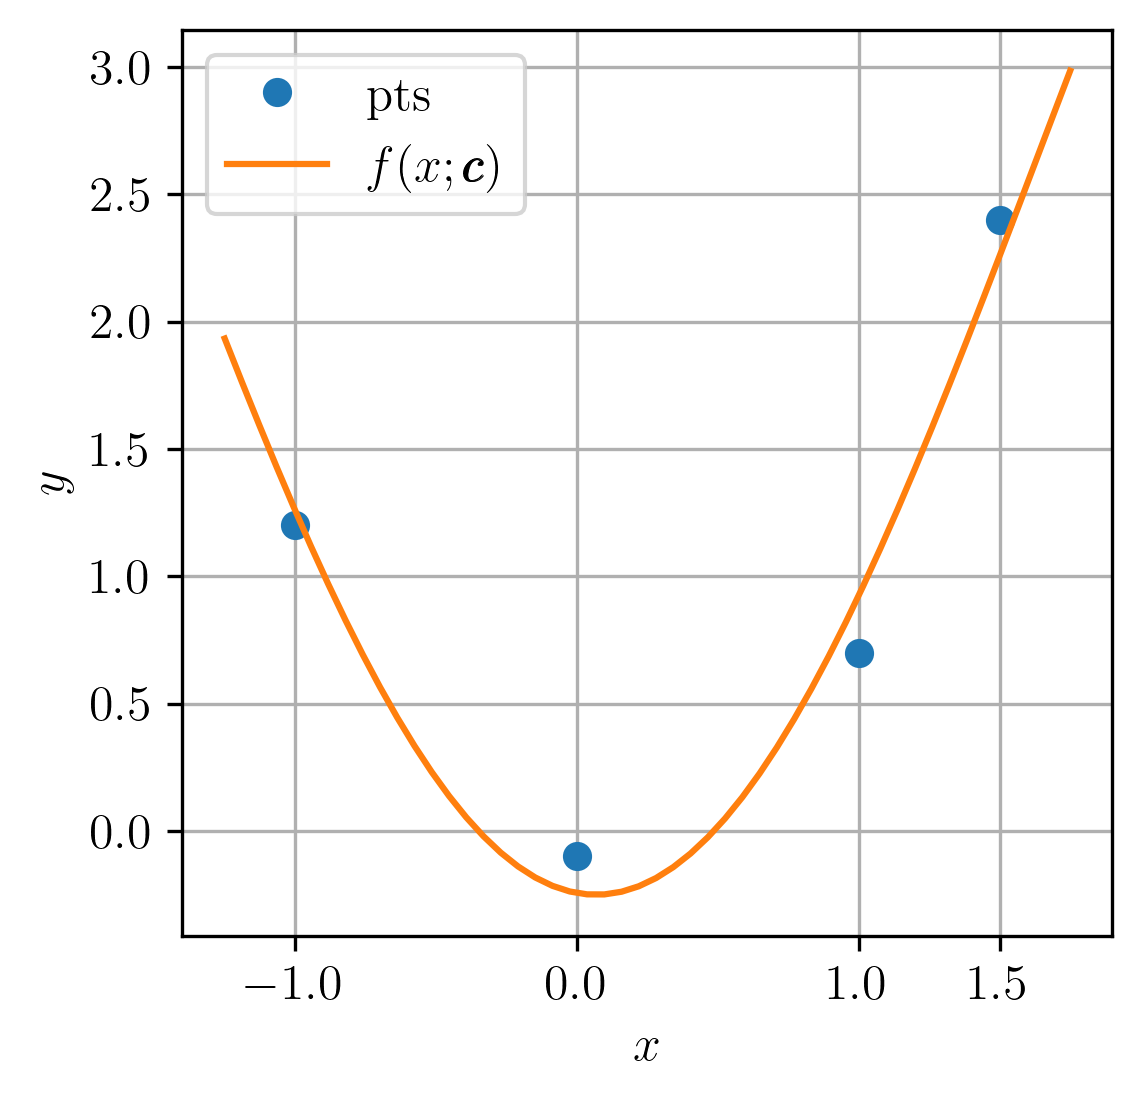
\includegraphics[width=4in]{cap_ajuste/dados/fig_mqCurva/fig.png}
    \caption{Curva ajustada no Exemplo~\ref{cap_ajuste_sec_prob_lin:ex:ajuste_de_curvas}.}
    \label{cap_ajuste_sec_prob_lin:fig:ex_ajuste_de_curvas}
  \end{figure}

\begin{lstlisting}[caption=mqCurva.py]
import numpy as np
import numpy.linalg as npla

# dados
xx = np.array([-1.0, 0.0, 1.0, 1.5])
yy = np.array([1.2, -0.1, 0.7, 2.4])

# matriz
m = 3
n = xx.size
A = np.empty((n,m))
A[:,0] = np.sin(xx)
A[:,1] = np.cos(xx)
A[:,2] = np.ones_like(xx)

# sol de mq
c = npla.solve(A.T@A, A.T@yy)

def f(x, c=c):
    y = c[0]*np.sin(x) \
      + c[1]*np.cos(x) \
      + c[2]
    return y
\end{lstlisting}

\end{ex}

\begin{ex}[\hl{Um Problema Não-Linear}]\label{cap_ajuste_sec_prob_lin:ex:mq_nlin0}
  Consideramos o problema de ajustar, no sentido de mínimos quadrados, a função
  \begin{equation}
    f(x; \pmb{c}) = c_1e^{c_2x}
  \end{equation}
  ao seguinte conjunto de pontos
  \begin{center}
    \begin{tabular}{lrr}
      $i$ & $x_i$ & $y_i$\\\midrule
      $1$ & $-1.0$ & $8.0$\\
      $2$ &  $0.0$ & $1.5$\\
      $3$ &  $1.0$ & $0.2$\\
      $4$ &  $1.5$ & $0.1$\\\bottomrule           
    \end{tabular}
  \end{center}

Aqui, temos um problema não linear de mínimos quadrados que pode ser transformado em um problema linear fazendo-se
\begin{align}
  & y = c_1e^{c_2x}\\
  & \ln y = \ln c_1e^{c_2x}\\
  & \ln y = \ln c_1 + c_2x.
\end{align}
Isto é, denotando $d_1 := \ln c_1$ e $d_2 := c_2$, o problema se resume a ajustar uma reta $r(x) = d_1 + d_2x$ ao conjunto de pontos $\{(x_i, \ln y_i)\}_{i=1}^4$.

Para resolver o problema transformado, formamos a matriz
\begin{equation}
  A :=
  \begin{bmatrix}
    1 & x_1 \\
    1 & x_2 \\
    1 & x_3 \\
    1 & x_4
  \end{bmatrix}
\end{equation}
e, então, resolvemos as equações normais $A^TA\pmb{d} = A^T\ln\pmb{y}$, com $\ln\pmb{y} = (\ln y_1, \ln y_2, \ln y_3, \ln y_4)$, donde obtemos $d_1 = 0.315$ e $d_2 = -1.792$. Das definições de $d_1$ e $d_2$, temos
\begin{align}
  &c_2 = d_2 = -1.792\\
  &c_1 = e^{d_1} = 1.371.
\end{align}
A Figura~\ref{cap_ajuste_sec_prob_lin:fig:ex_mq_nlin0} mostra um esboço da curva $f(x; \pmb{c}) = c_1e^{c_2x}$ ajustada aos pontos dados.

\begin{figure}[htb]
  \centering
  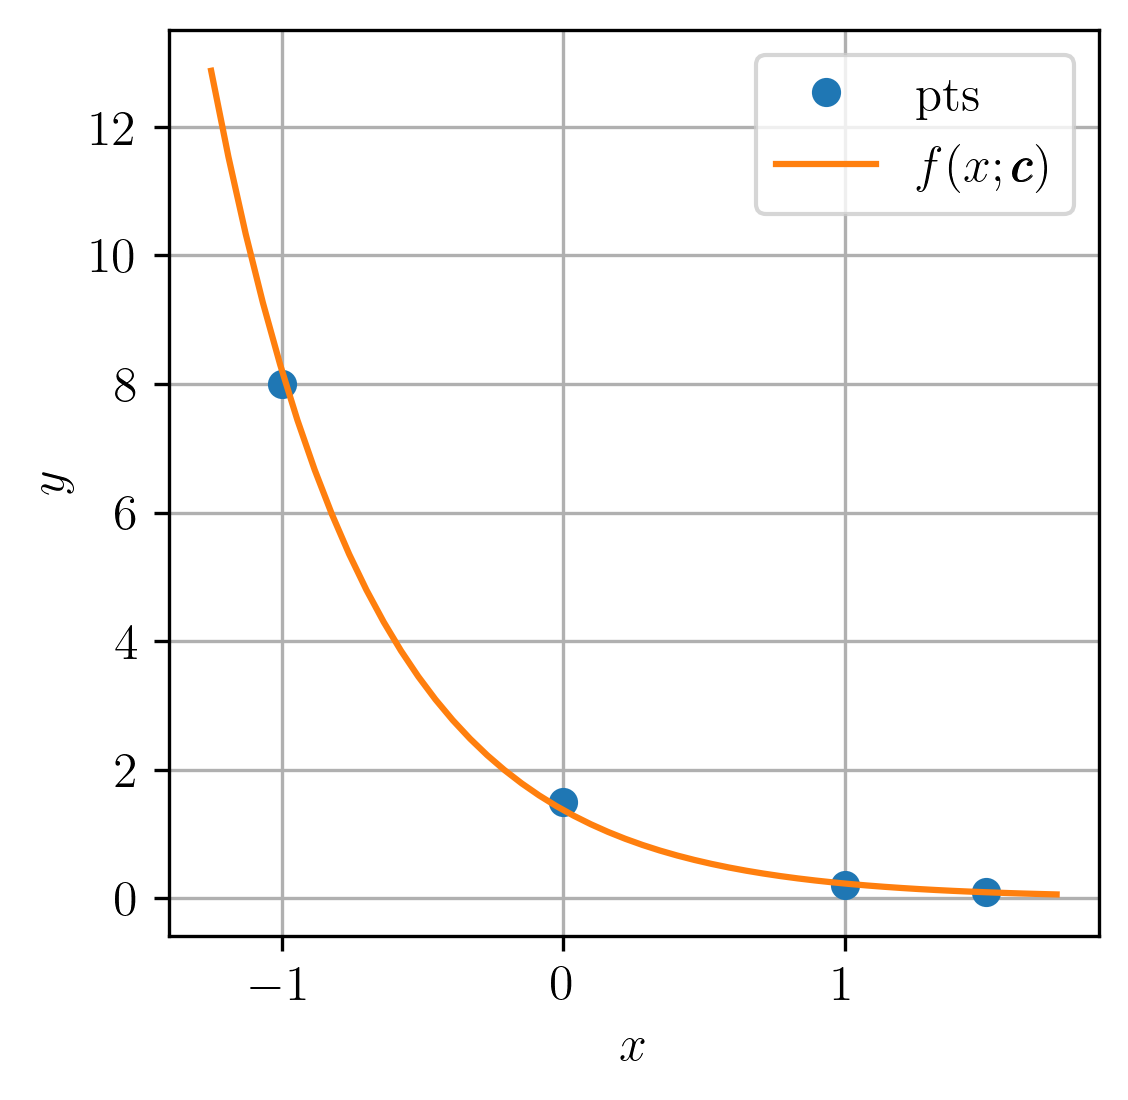
\includegraphics[width=4in]{cap_ajuste/dados/fig_mqUmPNLin/fig.png}
  \caption{Curva ajustada no Exemplo~\ref{cap_ajuste_sec_prob_lin:ex:mq_nlin0}.}
  \label{cap_ajuste_sec_prob_lin:fig:ex_mq_nlin0}
\end{figure}

\end{ex}

\subsection{Análise Numérica}
\badgeRevisar

O problema linear de mínimos quadrados~\eqref{cap_ajuste_sec_prob_lin:eq:pmq} reduz-se a resolver o sistema linear \eqref{cap_ajuste_sec_prob_lin:eq:equacoes_normais} para $\pmb{c}$. Isto nos leva a questão de verificar se $A^TA$ é invertível.

\begin{teo}
  A matriz $A^TA$ é positiva definida se, e somente se, as colunas de $A$ são linearmente independentes.
\end{teo}
\begin{dem}
  Se as colunas de $A$ são linearmente independentes, então $x\neq 0$ implica $Ax\neq 0$ e, equivalentemente, $x^TA^T\neq 0$. Portanto, $x\neq 0$ implica $x^TA^TAx = \|Ax\|_2^2 > 0$, o que mostra que $A^TA$ é positiva definida.

  Suponhamos, agora, que as colunas de $A$ não são linearmente independentes. Então, existe $x_0\neq 0$ tal que $Ax_0 = 0$. Mas, então, $x_0^TA^TAx_0=0$, o que mostra que $A^TA$ não é positiva definida. 
\end{dem}

Este teorema nos fornece uma condição suficiente para a existência (e unicidade) de solução do problema linear de mínimos quadrados. Mais especificamente, se as colunas da matriz $A$ são linearmente independentes, então os coeficientes da função $f(x)$ que melhor ajustam os pontos dados são
\begin{equation}
  c = (A^TA)^{-1}A^Ty.
\end{equation}

\subsection{Exercícios}

\begin{exer}
  Determine a reta $y = c_1x + c_2$ que melhor se ajusta, no sentido de mínimos quadrados, aos pontos
  \begin{center}
    \begin{tabular}{l|ccccc}
      $i$ & $1$ & $2$ & $3$ & $4$ & $5$ \\\hline
      $x_i$ & $-2.5$ & $-1.3$ & $0.2$ & $1.7$ & $2.3$\\
      $y_i$ & $3.8$ & $1.5$ & $-0.7$ & $-1.5$ & $-3.2$\\\hline
    \end{tabular}
  \end{center}
Por fim, compute a norma $L^2$ do resíduo, i.e. $\|r(c)\|_2 = \|y - (c_1x + c_2)\|_2$ para os pontos dados.
\end{exer}
\begin{resp}
  $c_1 = -1.3259$, $c_2 = 8.66071\E{-2}$, $\|r(c)\|_2 = 1.01390$.
\end{resp}

\begin{exer}
  Determine o polinômio $y = c_1x^3 + c_2x^2 + c_3x + c_4$ que melhor se ajusta, no sentido de mínimos quadrados, aos pontos
  \begin{center}
    \begin{tabular}{l|ccccc}
      $i$ & $1$ & $2$ & $3$ & $4$ & $5$ \\\hline
      $x_i$ & $-2.5$ & $-1.3$ & $0.2$ & $1.7$ & $2.3$\\
      $y_i$ & $3.8$ & $0.5$ & $2.7$ & $1.2$ & $-1.3$\\\hline
    \end{tabular}
  \end{center}
Por fim, compute a norma $L^2$ do resíduo, i.e. $\|r(c)\|_2$.
\end{exer}
\begin{resp}
  $c_1 = -4.50361\E{-1}$, $c_2 = -2.78350\E{-1}$, $c_3 = 1.46291$, $c_4 = 2.09648$, $\|r(c)\|_2 = 5.71346\E{-1}$
\end{resp}

\begin{exer}
  Determine a curva $y = c_1\sen x + c_2\cos x + c_3$ que melhor se ajusta, no sentido de mínimos quadrados, aos pontos
  \begin{center}
    \begin{tabular}{l|ccccc}
      $i$ & $1$ & $2$ & $3$ & $4$ & $5$ \\\hline
      $x_i$ & $-2.5$ & $-1.3$ & $0.2$ & $1.7$ & $2.3$\\
      $y_i$ & $3.8$ & $0.5$ & $2.7$ & $1.2$ & $-1.3$\\\hline
    \end{tabular}
  \end{center}
Por fim, compute a norma $L^2$ do resíduo, i.e. $\|r(c)\|_2$.
\end{exer}
\begin{resp}
  $c_1 = -0.86290414$, $c_2 = 0.36547042$, $c_3 = 1.4700346$, $\|r(c)\|_2 = 3.616409$
\end{resp}

\begin{exer}
  Use a transformação $z = \ln y$ para ajustar, no sentido de mínimos quadrados, a curva $y = c_1e^{c_2(x-c_3)^2}$ aos pontos
  \begin{center}
    \begin{tabular}{l|cccccc}
      $i$ & $1$ & $2$ & $3$ & $4$ & $5$ & $6$ \\\hline
      $x_i$ & $-0.5$ & $0.5$ & $1.3$ & $2,1$ & $2.7$ & $3,1$ \\
      $y_i$ & $0,1$ & $1.2$ & $2.7$ & $0.9$ & $0.2$ & $0,1$ \\\hline
    \end{tabular}
  \end{center}
\end{exer}
\begin{resp}
  $c_1 = 2.10131\E{+0}$, $c_2 = -9.73859\E{-1}$, $c_3 = 1.25521\E{+0}$
\end{resp}

\ifisbook
\subsubsection{Respostas}
\shipoutAnswer
\fi

%%% SECTION %%%
   
\section{Problemas Não Lineares}\label{cap_ajuste_sec_prob_nlin}
\badgeRevisar

Um \hl{problema não linear de mínimos quadrados consiste em ajustar} uma dada função 
\begin{equation}\hleq
  y = f(x; \pmb{c}) 
\end{equation}
\hl{que dependa não linearmente dos parâmetros $\pmb{c} = (c_1, c_2, \dotsc, c_m)$, $m\geq 1$, a um dado conjunto de $n\geq m$ pontos $\{(x_i, y_i)\}_{i=1}^n$}. Mais especificamente, buscamos resolver o seguinte \emph{problema de minimização}
\begin{equation}\label{eq:prob_nlin_mq}\hleq
  \min_{\{c_1, c_2, \dotsc, c_m\}} \left[E := \sum_{i=1}^n \left(y_i - f(x_i;c)\right)^2\right].
\end{equation}
Aqui, denotaremos por $r(c\pmb{)} := (r_1(\pmb{c}), r_2(\pmb{c}), \dotsc, r_n(\pmb{c}))$ o \emph{vetor dos resíduos} $r_i(\pmb{c}) := y_i - f(x_i, \pmb{c})$. Com isso, o problema se resume a encontrar o vetor de parâmetros $\pmb{c}$ que minimiza
\begin{equation}
  E = \|r(\pmb{c})\|^2.
\end{equation}

Tais parâmetros são solução do seguinte sistema de equações
\begin{equation}
  \frac{\p E}{\p c_j} = 2\sum_{i=1}^n r_i(\pmb{c})\frac{\p}{\p c_j}r_i(\pmb{c}) = 0
\end{equation}
ou, equivalentemente, da equação
\begin{equation}\label{eq:grad_E}
  \nabla E = 0 \Leftrightarrow J_R^T(\pmb{c})r(\pmb{c}) = 0,
\end{equation}
onde
\begin{equation}
  J_R(\pmb{c}) :=
  \begin{bmatrix}
    \frac{\p r_1}{\p c_1} & \frac{\p r_1}{\p c_2} & \cdots & \frac{\p r_1}{\p c_m}\\
    \frac{\p r_2}{\p c_1} & \frac{\p r_2}{\p c_2} & \cdots & \frac{\p r_2}{\p c_m}\\
    \vdots  & \vdots & \vdots & \vdots \\
    \frac{\p r_n}{\p c_1} & \frac{\p r_n}{\p c_2} & \cdots & \frac{\p r_n}{\p c_m}
  \end{bmatrix}
\end{equation}
é a jacobiana do resíduo $r$ em relação aos parâmetros $\pmb{c}$.

Podemos usar o método de Newton para resolver~\eqref{eq:grad_E}. Para tanto, escolhemos uma aproximação inicial para $\pmb{c}^{(1)} = (c_1^{(1)}, c_2^{(1)}, \dotsc, c_m^{(1)})$ e iteramos
\begin{align}
  H_R(c^{(k)})\delta^{(k)} &= -J_R^T(c)r(c) \label{eq:mqnl_newton1}\\
  c^{(k+1)} &= c^{(k)} + \delta^{(k)} \label{eq:mqnl_newton2},
\end{align}
onde $\delta^{(k)} = (\delta_1^{(k)}, \delta_2^{(k)}, \delta_m^{(k)})$ é a atualização de Newton (ou direção de busca) e $H_R(c) := [h_{p,q}(c)]_{p,q=1}^{m,m}$ é a matriz hessiana, cujos elementos são
\begin{equation}
  h_{p,q} := \sum_{i=1}^n\left\{\frac{\p r_i}{\p c_q}\frac{\p r_i}{\p c_p} + r_i\frac{\p^2 r_i}{\p c_q\p c_p}\right\}.
\end{equation}

\begin{ex}\label{ex:mqnl_newton}
  Consideremos o problema de ajustar, no sentido de mínimos quadrados, a função
  \begin{equation}
    f(x;c) = c_1e^{c_2x}
  \end{equation}
ao seguinte conjunto de pontos
\begin{center}
  \begin{tabular}{l|rrrr}
    $i$ & $1$ & $2$ & $3$ & $4$ \\\hline
    $x_i$ & $-1$ & $0$ & $1$ & $1.5$\\
    $y_i$ & $8.0$ & $1.5$ & $0.2$ & $0.1$\\\hline
  \end{tabular}
\end{center}

Aqui, vamos utilizar a iteração de Newton para o problema de mínimos quadrados, i.e. a iteração dada em \eqref{eq:mqnl_newton1}-\eqref{eq:mqnl_newton2}. Para tanto, para cada $i=1, 2, 3, 4$, precisamos das seguintes derivadas parciais do resíduo $r_i(c) := y_i - c_1e^{c_2x_i}$:
\begin{align}
  &\frac{\p}{\p c_1}r_i(c) = - e^{c_2x_i},\\
  &\frac{\p}{\p c_2}r_i(c) = - c_1x_ie^{c_2x_i},\\
  &\frac{\p^2}{\p c_1^2}r_i(c) = 0,\\
  &\frac{\p^2}{\p c_1\p c_2}r_i(c) = \frac{\p^2}{\p c_2\p c_1}r_i(c) = - x_ie^{c_2x_i},\\
  &\frac{\p^2}{\p c_2^2}r_i(c) = - c_1x_i^2e^{c_2x_i}.
\end{align}

\begin{figure}[h]
  \centering
  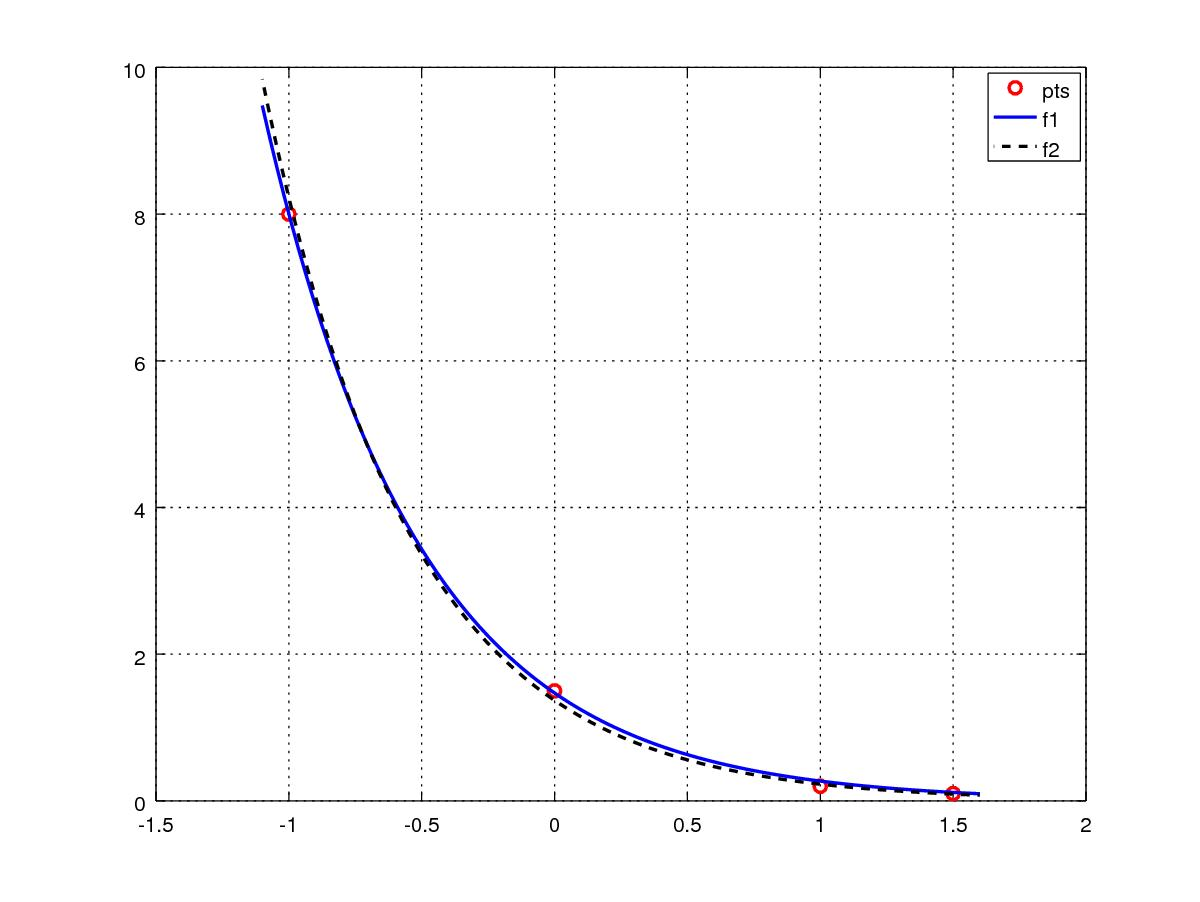
\includegraphics[width=\textwidth]{cap_ajuste/dados/ex_mqnl_N/ex_mqnl_N}
  \caption{Esboço da curva ajustada no Exemplo~\ref{ex:mqnl_newton}.}
  \label{fig:ex_mqnl_newton}
\end{figure}

Com isso e tomando $c^{(1)} = (1.4,  -1.8)$ (motivado do Exemplo~\ref{ex:mq_nlin0}), computamos as iterações de Newton~\eqref{eq:mqnl_newton1}-\eqref{eq:mqnl_newton2}. Iterando até a precisão de $TOL = 10^{-4}$, obtemos a solução $c_1 = 1.471$ e $c_2 = -1.6938$. Na Figura~\ref{fig:ex_mqnl_newton} vemos uma comparação entre a curva aqui ajustada ($-$) e aquela obtida no Exemplo~\ref{ex:mq_nlin0} ($--$).

% \ifisoctave
% O ajuste discutido neste exemplo pode ser computado no \verb+GNU Octave+ com o seguinte código:
% \begin{verbatim}
% #pontos
% global x = [-1 0 1 1.5]';
% global y = [8.0 1.5 0.2 0.1]';

% #fun. objetivo
% f = @(x,c) c(1)*exp(c(2)*x);

% #residuo
% r = @(c) y - f(x,c);

% #jacobiana
% function A = J(c)
%   global x
%   A = zeros(4,2);
%   A(:,1) = - exp(c(2)*x);
%   A(:,2) = - c(1)*x.*exp(c(2)*x);
% endfunction

% #hessiana
% function A = H(c)
%   global x
%   global y
%   A = zeros(2,2);
%   A = J(c)'*J(c);
%   for i=1:4
%     A(1,1) += 0;
%     A(1,2) += (y(i) - c(1)*exp(c(2)*x(i))) * ...
%               (- x(i)*exp(c(2)*x(i)));
%     A(2,1) += (y(i) - c(1)*exp(c(2)*x(i))) * ...
%               (- x(i)*exp(c(2)*x(i)));
%     A(2,2) += (y(i) - c(1)*exp(c(2)*x(i))) * ...
%               (- c(1)*x(i)^2*exp(c(2)*x(i)));
%   endfor
% endfunction

% #aprox. inicial
% c = [1.4 -1.8]';

% #iteracoes de Newton
% k=0;
% do
%   k+=1;
%   delta = - inv(H(c))*J(c)'*r(c);
%   c = c + delta;
%   [k,c',norm(delta)]
% until ((k>10) | (norm(delta)<1e-4))
% \end{verbatim}
% \fi
\end{ex}

Observamos que a solução obtida no exemplo anterior (Exemplo~\ref{ex:mqnl_newton}) difere da previamente encontrada no Exemplo~\ref{ex:mq_nlin0}. Naquele exemplo, os parâmetros obtidos nos fornecem $E = 6.8\E{-2}$, enquanto que a solução do exemplo anterior fornece $E = 6.1\E{-3}$. Isto é esperado, pois naquele exemplo resolvemos um problema aproximado, enquanto no exemplo anterior resolvemos o problema por si.

O emprego do método de Newton para o problema de mínimos quadrados tem a vantagem da taxa de convergência quadrática, entretanto requer a computação das derivadas parciais de segunda ordem do resíduo. Na sequência discutimos alternativas comumente empregadas.

\subsection{Método de Gauss-Newton}
\badgeRevisar

O método de Gauss-Newton é uma técnica iterativa que aproxima o problema não linear de mínimos quadrados \eqref{eq:prob_nlin_mq} por uma sequência de problemas lineares. Para seu desenvolvimento, começamos de uma aproximação inicial $c^{(1)} = (c_1^{(1)}, c_2^{(1)}, \dotsc, c_m^{(1)})$ dos parâmetros que queremos ajustar. Também, assumindo que a $n$-ésima iterada $c^{(k)}$ é conhecida, faremos uso da aproximação de primeira ordem de $f(x,c)$ por polinômio de Taylor, i.e.
\begin{equation}
  f(x;c^{(k+1)}) \approx f(x;c^{(k)}) + \nabla_c f(x;c^{(k)})(c^{(k+1)}-c^{(k)}),
\end{equation}
onde
\begin{equation}
  \nabla_c f(x;c) = \left[\frac{\p}{\p c_1}f(x;c) ~\frac{\p}{\p c_2}f(x;c) ~\cdots ~\frac{\p}{\p c_m}f(x;c)\right].
\end{equation}

O método consiste em obter a solução do problema não linear \eqref{eq:prob_nlin_mq} pelo limite dos seguintes problemas lineares de mínimos quadrados
\begin{align}
  \min_{\delta^{(k)}} &\left[\tilde{E} := \sum_{i=1}^n (y_i - f(x_i,c^{(k)}) - \nabla_c f(x_i;c^{(k)})\delta^{(k)})^2\right] \label{eq:mq_gn0}\\
  &c^{(k+1)} = c^{(k)} + \delta^{(k)}.
\end{align}

Agora, usando a notação de resíduo $r(c) = y - f(x;c)$, observamos que \eqref{eq:mq_gn0} consiste no problema linear de mínimos quadrados
\begin{equation}
  \min_{\delta^{(k)}} \|r(c^{(k)}) + J_R(c^{(k)})\delta^{(k)}\|_2^2,
\end{equation}
o qual é equivalente a resolver as equações normais
\begin{equation}
  J_R^T(c^{(n)})J_R(c^{(n)})\delta^{(n)} = -J_R^T(c)r(c).
\end{equation}

Com isso, dada uma aproximação inicial $c^{(1)}$, a \emph{iteração do método de Gauss-Newton} consiste em
\begin{align}
  &J_R^T(c^{(k)})J_R(c^{(k)})\delta^{(k)} = -J_R^T(c)r(c)\\
  &c^{(k+1)} = c^{(k)} + \delta^{(k)}.
\end{align}

\begin{ex}
  A aplicação da iteração de Gauss-Newton ao problema de mínimos quadrados discutido no Exemplo~\ref{ex:mqnl_newton} nos fornece a mesma solução obtida naquele exemplo (preservadas a aproximação inicial e a tolerância de precisão).

% \ifisoctave
% A implementação do método de Gauss-Newton para este problema no \verb+GNU Octave+ pode ser feita com o seguinte código:
% \begin{verbatim}
% #pontos
% global x = [-1 0 1 1.5]';
% y = [8.0 1.5 0.2 0.1]';

% #fun. objetivo
% f = @(x,c) c(1)*exp(c(2)*x);

% #residuo
% r = @(c) y - f(x,c);

% #jacobiana
% function A = J(c)
%   global x
%   A = zeros(4,2);
%   A(:,1) = - exp(c(2)*x);
%   A(:,2) = - c(1)*x.*exp(c(2)*x);
% endfunction

% #aprox. inicial
% c = [1.4 -1.8]';

% #iteracoes de Gauss-Newton
% k=0;
% do
%   k+=1;
%   delta = - inv(J(c)'*J(c))*J(c)'*r(c);
%   c = c + delta;
%   [k,c',norm(delta)]
% until ((k>10) | (norm(delta)<1e-4))
% \end{verbatim}
% \fi
\end{ex}

O método de Gauss-Newton pode ser lentamente convergente para problemas muito não lineares ou com resíduos grandes. Nesse caso, métodos de Gauss-Newton com amortecimento são alternativas robustas~\cite{Bjorck1996a,Nocedal2006a}. Na sequência, introduziremos um destes métodos, conhecido como método de Levenberg-Marquardt.

\subsection{Método de Levenberg-Marquardt}
\badgeRevisar

O método de Levenberg-Marquardt é uma variação do método de Gauss-Newton no qual a direção de busca $\delta^{(n)}$ é obtida da solução do seguinte problema regularizado
\begin{equation} \label{eq:mq_gn0}
  \min_{\delta^{(k)}} \{\|r(c^{(k)}) + J_R(c^{(k)})\delta^{(k)}\|_2^2 + \mu^{(k)}\|\delta^{(k)}\|_2^2\}
\end{equation}
ou, equivalentemente,
\begin{equation} \label{eq:mq_gn0}
  \min_{\delta^{(k)}} \left\|
    \begin{bmatrix}
      r(c^{(k)})\\
      0
    \end{bmatrix} +
    \begin{bmatrix}
      J_R(c^{(k)})\\
      \mu^{(k)}I
    \end{bmatrix}
    \delta^{(k)}\right\|_2^2
\end{equation}

A taxa de convergência das iterações de Levenberg-Marquardt é sensível a escolha do parâmetro $\mu^{(k)}\geq 0$. Aqui, faremos esta escolha por tentativa e erro. O leitor pode aprofundar-se mais sobre esta questão na literatura especializada (veja, por exemplo, \cite{Bjorck1996a,Nocedal2006a}).

\begin{obs}
  Quando $\mu^{(k)} \equiv 0$ para todo $n$, o método de Levenberg-Marquardt é equivalente ao método de Gauss-Newton.
\end{obs}

\begin{ex}\label{ex:mqnl_LM}
  Consideremos o problema de mínimos quadrados discutido no Exemplo~\ref{ex:mqnl_newton}. O método de Gauss-Newton falha para este problema se escolhermos, por exemplo, $c^{(1)} = (0, 0)$. Isto ocorre pois, para esta escolha de $c^{(1)}$, a jacobiana $J(c^{(1)})$ não tem posto completo. Entretanto, o método de Levenberg-Marquardt com $\mu^{(k)} = 0.1$ é convergente, mesmo para esta escolha de $c^{(1)}$.

% \ifisoctave
% A implementação no \verb+GNU Octave+ do método de Levenberg-Marquardt (com $\mu^{(k)}=0,1$ constante) para este problema pode ser feita com o seguinte código:
% \begin{verbatim}
% #pontos
% global x = [-1 0 1 1.5]';
% y = [8.0 1.5 0.2 0.1]';

% #fun. objetivo
% f = @(x,c) c(1)*exp(c(2)*x);

% #residuo
% r = @(c) y - f(x,c);

% #jacobiana
% function A = JR(c)
%   global x;
%   A = zeros(4,2);
%   A(:,1) = - exp(c(2)*x);
%   A(:,2) = - c(1)*x.*exp(c(2)*x);
% endfunction

% #aprox. inicial
% c = [0 0]';

% #param. de amortecimento
% mu = 0.1;

% #iteracoes de Gauss-Newton
% k=0;
% do
%   k+=1;
%   JJ = [JR(c);mu*eye(2,2)];
%   delta = - inv(JJ'*JJ)*JJ'*[r(c);zeros(2,1)];
%   c = c + delta;
%   printf("%d %1.1e %1.3e %1.3e\n", k,norm(delta),c')
% until ((k>10) | (norm(delta)<1e-4))
% \end{verbatim}
% \fi
\end{ex}

\subsection{Exercícios}
\badgeRevisar

\begin{exer}\label{exer:mqnl_GN}
  Use o método de Gauss-Newton para ajustar, no sentido de mínimos quadrados e com precisão de $10^{-4}$, a curva $y = c_1e^{c_2(x-c_3)^2}$ aos pontos
  \begin{center}
    \begin{tabular}{l|cccccc}
      $i$ & $1$ & $2$ & $3$ & $4$ & $5$ & $6$ \\\hline
      $x_i$ & $-0.5$ & $0.5$ & $1.3$ & $2.1$ & $2.7$ & $3.1$ \\
      $y_i$ & $0.1$ & $1.2$ & $2.7$ & $0.9$ & $0.2$ & $0.1$ \\\hline
    \end{tabular}
  \end{center}
Use as condições iniciais:
\begin{enumerate}[a)]
\item $c_1 = 2.1$, $c_2=-1$ e $c_3=1.3$.
\item $c_1=1$, $c_2=-1$ e $c_3=-1$.
\end{enumerate}
\end{exer}
\begin{resp}
  % \ifisoctave 
  % \href{https://github.com/phkonzen/notas/blob/master/src/MatematicaNumerica/cap_ajuste/dados/exer_mqnl_GN/exer_mqnl_GN.m}{Código.} 
  % \fi
  a) $c_1 = 2.69971\E{+0}$, $c_2 = -1.44723\E{+0}$, $c_3 = 1.24333\E{+0}$; b) divergente.
\end{resp}

\begin{exer}
  Resolva o exercício anterior (Exercício~\ref{exer:mqnl_GN}) usando o método de Levenberg-Marquardt com amortecimento constante $\mu=0.2$.
\end{exer}
\begin{resp}
  % \ifisoctave 
  % \href{https://github.com/phkonzen/notas/blob/master/src/MatematicaNumerica/cap_ajuste/dados/exer_mqnl_LM/exer_mqnl_LM.m}{Código.} 
  % \fi
  a)  $c_1 = 2.69971\E{+0}$, $c_2 = -1.44723\E{+0}$, $c_3 = 1.24333\E{+0}$; b) $c_1 = 2.69971\E{+0}$, $c_2 = -1.44723\E{+0}$, $c_3 = 1.24333\E{+0}$
\end{resp}

\ifisbook
\subsubsection{Respostas}
\shipoutAnswer
\fi

%%% SECTION %%%


% endnotes
\clearpage
\phantomsection
\addcontentsline{toc}{chapter}{Notas}
\theendnotes

% bibliografia
\ifisbook
\clearpage
\phantomsection
\renewcommand\bibname{Referências}
\addcontentsline{toc}{chapter}{\bibname}
\fi

\begin{thebibliography}{99}
\bibitem{Bjorck1996a}
  Björk, A.. Numerical Methods for Least Squares Problems. SIAM, 1996.

\bibitem{Burden2016a}
  Burden, R.L.; Faires, J.D.; Burden, A.M.. Análise Numérica. 3. ed., Cengage Learning, 2016. ISBN: \texttt{978-8522123414}. Acesso \href{https://bit.ly/3XB54MJ}{SABI+UFRGS}.

\bibitem{Isaacson1994a}
  Isaacson, E.; Keller H.B.. Analysis of Numerical Methods. Dover, 1994.

\bibitem{Lemire2021a}
  Lemire, D.. Number Parsing at a Gigabyte per Second. Software: Practice and Experience, 51(8), 2021, 1700-1727. DOI: \href{https://doi.org/10.1002/spe.2984}{10.1002/spe.2984}.

\bibitem{Nocedal2006a}
  Nocedal, J.; Wright, S.J.. Numerical Optimization. Springer, 2006.

\bibitem{Press2007a}
  Press, W.H.; Teukolsky, S.A.; Vetterling, W.T.; Flannery, B.P.. Numerical Recipes. 3. ed., Cambridge University Press,
2007.

\bibitem{Ralston2001a}
  Ralston, A.; Rabinowitz, P.. A First Course in Numerical Analysis. 2. ed., Dover: New York, 2021. ISBN \texttt{048641454X}.

\bibitem{Stoer1993a}
  Stoer, J.; Bulirsch, R.. Introduction to numerical analysis. 2. ed., Springer-Verlag, 1993.
\end{thebibliography}

% índice
\ifisbook
\printindex
\fi


\end{document}
